\documentclass[twoside]{book}

% Packages required by doxygen
\usepackage{fixltx2e}
\usepackage{calc}
\usepackage{doxygen}
\usepackage[export]{adjustbox} % also loads graphicx
\usepackage{graphicx}
\usepackage[utf8]{inputenc}
\usepackage{makeidx}
\usepackage{multicol}
\usepackage{multirow}
\PassOptionsToPackage{warn}{textcomp}
\usepackage{textcomp}
\usepackage[nointegrals]{wasysym}
\usepackage[table]{xcolor}

% Font selection
\usepackage[T1]{fontenc}
\usepackage[scaled=.90]{helvet}
\usepackage{courier}
\usepackage{amssymb}
\usepackage{sectsty}
\renewcommand{\familydefault}{\sfdefault}
\allsectionsfont{%
  \fontseries{bc}\selectfont%
  \color{darkgray}%
}
\renewcommand{\DoxyLabelFont}{%
  \fontseries{bc}\selectfont%
  \color{darkgray}%
}
\newcommand{\+}{\discretionary{\mbox{\scriptsize$\hookleftarrow$}}{}{}}

% Page & text layout
\usepackage{geometry}
\geometry{%
  a4paper,%
  top=2.5cm,%
  bottom=2.5cm,%
  left=2.5cm,%
  right=2.5cm%
}
\tolerance=750
\hfuzz=15pt
\hbadness=750
\setlength{\emergencystretch}{15pt}
\setlength{\parindent}{0cm}
\setlength{\parskip}{3ex plus 2ex minus 2ex}
\makeatletter
\renewcommand{\paragraph}{%
  \@startsection{paragraph}{4}{0ex}{-1.0ex}{1.0ex}{%
    \normalfont\normalsize\bfseries\SS@parafont%
  }%
}
\renewcommand{\subparagraph}{%
  \@startsection{subparagraph}{5}{0ex}{-1.0ex}{1.0ex}{%
    \normalfont\normalsize\bfseries\SS@subparafont%
  }%
}
\makeatother

% Headers & footers
\usepackage{fancyhdr}
\pagestyle{fancyplain}
\fancyhead[LE]{\fancyplain{}{\bfseries\thepage}}
\fancyhead[CE]{\fancyplain{}{}}
\fancyhead[RE]{\fancyplain{}{\bfseries\leftmark}}
\fancyhead[LO]{\fancyplain{}{\bfseries\rightmark}}
\fancyhead[CO]{\fancyplain{}{}}
\fancyhead[RO]{\fancyplain{}{\bfseries\thepage}}
\fancyfoot[LE]{\fancyplain{}{}}
\fancyfoot[CE]{\fancyplain{}{}}
\fancyfoot[RE]{\fancyplain{}{\bfseries\scriptsize Generated by Doxygen }}
\fancyfoot[LO]{\fancyplain{}{\bfseries\scriptsize Generated by Doxygen }}
\fancyfoot[CO]{\fancyplain{}{}}
\fancyfoot[RO]{\fancyplain{}{}}
\renewcommand{\footrulewidth}{0.4pt}
\renewcommand{\chaptermark}[1]{%
  \markboth{#1}{}%
}
\renewcommand{\sectionmark}[1]{%
  \markright{\thesection\ #1}%
}

% Indices & bibliography
\usepackage{natbib}
\usepackage[titles]{tocloft}
\setcounter{tocdepth}{3}
\setcounter{secnumdepth}{5}
\makeindex

% Hyperlinks (required, but should be loaded last)
\usepackage{ifpdf}
\ifpdf
  \usepackage[pdftex,pagebackref=true]{hyperref}
\else
  \usepackage[ps2pdf,pagebackref=true]{hyperref}
\fi
\hypersetup{%
  colorlinks=true,%
  linkcolor=blue,%
  citecolor=blue,%
  unicode%
}

% Custom commands
\newcommand{\clearemptydoublepage}{%
  \newpage{\pagestyle{empty}\cleardoublepage}%
}

\usepackage{caption}
\captionsetup{labelsep=space,justification=centering,font={bf},singlelinecheck=off,skip=4pt,position=top}

%===== C O N T E N T S =====

\begin{document}

% Titlepage & ToC
\hypersetup{pageanchor=false,
             bookmarksnumbered=true,
             pdfencoding=unicode
            }
\pagenumbering{roman}
\begin{titlepage}
\vspace*{7cm}
\begin{center}%
{\Large E\+C\+E\+N5013 Project1 -\/ Gunj Manseta }\\
\vspace*{1cm}
{\large Generated by Doxygen 1.8.11}\\
\end{center}
\end{titlepage}
\clearemptydoublepage
\tableofcontents
\clearemptydoublepage
\pagenumbering{arabic}
\hypersetup{pageanchor=true}

%--- Begin generated contents ---
\chapter{E\+C\+E\+N5013 Project 1}
\label{index}\hypertarget{index}{}\subsection*{Author -\/ Gunj Manseta (Embedded Systems Engineering -\/ University of Colorado Boulder)}

\subsubsection*{A multithreaded console application for Beagle\+Bone black/green(Linux) having sensor interface, server, and logger}

\paragraph*{Code Documentation can be found at -\/ \href{http://htmlpreview.github.io/?https://github.com/mansetagunj/ECEN-5013/blob/master/Project1/documentation/doxygenfiles.d/html/index.html}{\tt Project Code Documentation webpage} (Ctrl+click for new tab)}

The project includes 1 parent thread which is the main task. The main task spawns 4 child threads


\begin{DoxyEnumerate}
\item Temperature sensor task which is responsible for talking with the T\+M\+P102 sensor.
\item Light sensor task which is responsible for talking with the A\+P\+D\+S9301 light sensor.
\item Socket task which is runs a T\+CP server and accepts connection from the client with various requests suchs as getting temperature and lux value from the sensor.
\item Logger task which is solely responsible for logging to a file setup in the config file.
\end{DoxyEnumerate}

The sensor tasks talks with the sensor via a M\+T-\/safe I2\+Cmaster wrapper written around the Intel open source project mraa library intended for various boards.

The main task which is the parent task keeps a check of the children task if they are alive or not and if any of the thread is found to be dead or stuck for more than the timeout set by in the config file, the main task closes all the threads and exits gracefully.

\subsubsection*{This project is intended to run on the Beagle\+Bone black/green."}
\chapter{Data Structure Index}
\section{Data Structures}
Here are the data structures with brief descriptions\+:\begin{DoxyCompactList}
\item\contentsline{section}{\hyperlink{unionREMOTE__RESPONSE__T_1_1data}{R\+E\+M\+O\+T\+E\+\_\+\+R\+E\+S\+P\+O\+N\+S\+E\+\_\+\+T\+::data} }{\pageref{unionREMOTE__RESPONSE__T_1_1data}}{}
\item\contentsline{section}{\hyperlink{structi2c__handle}{i2c\+\_\+handle} \\*This is the handle for I2C mster and each master should have only one handle }{\pageref{structi2c__handle}}{}
\item\contentsline{section}{\hyperlink{structLIGHTTASKQ__MSG__T}{L\+I\+G\+H\+T\+T\+A\+S\+K\+Q\+\_\+\+M\+S\+G\+\_\+T} }{\pageref{structLIGHTTASKQ__MSG__T}}{}
\item\contentsline{section}{\hyperlink{structLOGGERTASKQ__MSG__T}{L\+O\+G\+G\+E\+R\+T\+A\+S\+K\+Q\+\_\+\+M\+S\+G\+\_\+T} }{\pageref{structLOGGERTASKQ__MSG__T}}{}
\item\contentsline{section}{\hyperlink{structMAINTASKQ__MSG__T}{M\+A\+I\+N\+T\+A\+S\+K\+Q\+\_\+\+M\+S\+G\+\_\+T} }{\pageref{structMAINTASKQ__MSG__T}}{}
\item\contentsline{section}{\hyperlink{structOBJECT__PACKET__T}{O\+B\+J\+E\+C\+T\+\_\+\+P\+A\+C\+K\+E\+T\+\_\+T} }{\pageref{structOBJECT__PACKET__T}}{}
\item\contentsline{section}{\hyperlink{structREMOTE__REQUEST__T}{R\+E\+M\+O\+T\+E\+\_\+\+R\+E\+Q\+U\+E\+S\+T\+\_\+T} }{\pageref{structREMOTE__REQUEST__T}}{}
\item\contentsline{section}{\hyperlink{structREMOTE__RESPONSE__T}{R\+E\+M\+O\+T\+E\+\_\+\+R\+E\+S\+P\+O\+N\+S\+E\+\_\+T} }{\pageref{structREMOTE__RESPONSE__T}}{}
\item\contentsline{section}{\hyperlink{structTEMPERATURETASKQ__MSG__T}{T\+E\+M\+P\+E\+R\+A\+T\+U\+R\+E\+T\+A\+S\+K\+Q\+\_\+\+M\+S\+G\+\_\+T} }{\pageref{structTEMPERATURETASKQ__MSG__T}}{}
\item\contentsline{section}{\hyperlink{structTMP102__CONFIG__REG__SETTINGS__T}{T\+M\+P102\+\_\+\+C\+O\+N\+F\+I\+G\+\_\+\+R\+E\+G\+\_\+\+S\+E\+T\+T\+I\+N\+G\+S\+\_\+T} }{\pageref{structTMP102__CONFIG__REG__SETTINGS__T}}{}
\end{DoxyCompactList}

\chapter{File Index}
\section{File List}
Here is a list of all documented files with brief descriptions\+:\begin{DoxyCompactList}
\item\contentsline{section}{/home/gunj/repos/\+E\+C\+E\+N-\/5013/\+Project1/include/\+Beagle\+Bone/\hyperlink{apds9301__sensor_8h}{apds9301\+\_\+sensor.\+h} }{\pageref{apds9301__sensor_8h}}{}
\item\contentsline{section}{/home/gunj/repos/\+E\+C\+E\+N-\/5013/\+Project1/include/\+Beagle\+Bone/\hyperlink{BB__Led_8h}{B\+B\+\_\+\+Led.\+h} }{\pageref{BB__Led_8h}}{}
\item\contentsline{section}{/home/gunj/repos/\+E\+C\+E\+N-\/5013/\+Project1/include/\+Beagle\+Bone/\hyperlink{my__i2c_8h}{my\+\_\+i2c.\+h} }{\pageref{my__i2c_8h}}{}
\item\contentsline{section}{/home/gunj/repos/\+E\+C\+E\+N-\/5013/\+Project1/include/\+Beagle\+Bone/\hyperlink{tmp102__sensor_8h}{tmp102\+\_\+sensor.\+h} }{\pageref{tmp102__sensor_8h}}{}
\item\contentsline{section}{/home/gunj/repos/\+E\+C\+E\+N-\/5013/\+Project1/include/common/\hyperlink{common__helper_8h}{common\+\_\+helper.\+h} }{\pageref{common__helper_8h}}{}
\item\contentsline{section}{/home/gunj/repos/\+E\+C\+E\+N-\/5013/\+Project1/include/common/\hyperlink{error__data_8h}{error\+\_\+data.\+h} }{\pageref{error__data_8h}}{}
\item\contentsline{section}{/home/gunj/repos/\+E\+C\+E\+N-\/5013/\+Project1/include/common/\hyperlink{light__sensor__task_8h}{light\+\_\+sensor\+\_\+task.\+h} }{\pageref{light__sensor__task_8h}}{}
\item\contentsline{section}{/home/gunj/repos/\+E\+C\+E\+N-\/5013/\+Project1/include/common/\hyperlink{logger__task_8h}{logger\+\_\+task.\+h} }{\pageref{logger__task_8h}}{}
\item\contentsline{section}{/home/gunj/repos/\+E\+C\+E\+N-\/5013/\+Project1/include/common/\hyperlink{main__task_8h}{main\+\_\+task.\+h} }{\pageref{main__task_8h}}{}
\item\contentsline{section}{/home/gunj/repos/\+E\+C\+E\+N-\/5013/\+Project1/include/common/\hyperlink{my__signals_8h}{my\+\_\+signals.\+h} }{\pageref{my__signals_8h}}{}
\item\contentsline{section}{/home/gunj/repos/\+E\+C\+E\+N-\/5013/\+Project1/include/common/\hyperlink{my__time_8h}{my\+\_\+time.\+h} }{\pageref{my__time_8h}}{}
\item\contentsline{section}{/home/gunj/repos/\+E\+C\+E\+N-\/5013/\+Project1/include/common/\hyperlink{posixTimer_8h}{posix\+Timer.\+h} }{\pageref{posixTimer_8h}}{}
\item\contentsline{section}{/home/gunj/repos/\+E\+C\+E\+N-\/5013/\+Project1/include/common/\hyperlink{readConfiguration_8h}{read\+Configuration.\+h} }{\pageref{readConfiguration_8h}}{}
\item\contentsline{section}{/home/gunj/repos/\+E\+C\+E\+N-\/5013/\+Project1/include/common/\hyperlink{sensor__common__object_8h}{sensor\+\_\+common\+\_\+object.\+h} }{\pageref{sensor__common__object_8h}}{}
\item\contentsline{section}{/home/gunj/repos/\+E\+C\+E\+N-\/5013/\+Project1/include/common/\hyperlink{socket__task_8h}{socket\+\_\+task.\+h} }{\pageref{socket__task_8h}}{}
\item\contentsline{section}{/home/gunj/repos/\+E\+C\+E\+N-\/5013/\+Project1/include/common/\hyperlink{temperature__sensor__task_8h}{temperature\+\_\+sensor\+\_\+task.\+h} }{\pageref{temperature__sensor__task_8h}}{}
\item\contentsline{section}{/home/gunj/repos/\+E\+C\+E\+N-\/5013/\+Project1/src/\hyperlink{apds9301__sensor_8c}{apds9301\+\_\+sensor.\+c} }{\pageref{apds9301__sensor_8c}}{}
\item\contentsline{section}{/home/gunj/repos/\+E\+C\+E\+N-\/5013/\+Project1/src/\hyperlink{BB__Led_8c}{B\+B\+\_\+\+Led.\+c} }{\pageref{BB__Led_8c}}{}
\item\contentsline{section}{/home/gunj/repos/\+E\+C\+E\+N-\/5013/\+Project1/src/\hyperlink{common__helper_8c}{common\+\_\+helper.\+c} }{\pageref{common__helper_8c}}{}
\item\contentsline{section}{/home/gunj/repos/\+E\+C\+E\+N-\/5013/\+Project1/src/\hyperlink{light__sensor__task_8c}{light\+\_\+sensor\+\_\+task.\+c} }{\pageref{light__sensor__task_8c}}{}
\item\contentsline{section}{/home/gunj/repos/\+E\+C\+E\+N-\/5013/\+Project1/src/\hyperlink{logger__task_8c}{logger\+\_\+task.\+c} }{\pageref{logger__task_8c}}{}
\item\contentsline{section}{/home/gunj/repos/\+E\+C\+E\+N-\/5013/\+Project1/src/\hyperlink{main__task_8c}{main\+\_\+task.\+c} }{\pageref{main__task_8c}}{}
\item\contentsline{section}{/home/gunj/repos/\+E\+C\+E\+N-\/5013/\+Project1/src/\hyperlink{my__i2c_8c}{my\+\_\+i2c.\+c} }{\pageref{my__i2c_8c}}{}
\item\contentsline{section}{/home/gunj/repos/\+E\+C\+E\+N-\/5013/\+Project1/src/\hyperlink{my__signals_8c}{my\+\_\+signals.\+c} }{\pageref{my__signals_8c}}{}
\item\contentsline{section}{/home/gunj/repos/\+E\+C\+E\+N-\/5013/\+Project1/src/\hyperlink{my__time_8c}{my\+\_\+time.\+c} }{\pageref{my__time_8c}}{}
\item\contentsline{section}{/home/gunj/repos/\+E\+C\+E\+N-\/5013/\+Project1/src/\hyperlink{posixTimer_8c}{posix\+Timer.\+c} }{\pageref{posixTimer_8c}}{}
\item\contentsline{section}{/home/gunj/repos/\+E\+C\+E\+N-\/5013/\+Project1/src/\hyperlink{readConfiguration_8c}{read\+Configuration.\+c} }{\pageref{readConfiguration_8c}}{}
\item\contentsline{section}{/home/gunj/repos/\+E\+C\+E\+N-\/5013/\+Project1/src/\hyperlink{socket__task_8c}{socket\+\_\+task.\+c} }{\pageref{socket__task_8c}}{}
\item\contentsline{section}{/home/gunj/repos/\+E\+C\+E\+N-\/5013/\+Project1/src/\hyperlink{temperature__sensor__task_8c}{temperature\+\_\+sensor\+\_\+task.\+c} }{\pageref{temperature__sensor__task_8c}}{}
\item\contentsline{section}{/home/gunj/repos/\+E\+C\+E\+N-\/5013/\+Project1/tests/\+B\+B\+B\+\_\+\+User\+L\+E\+D\+\_\+\+Test/\hyperlink{LED__test_8c}{L\+E\+D\+\_\+test.\+c} }{\pageref{LED__test_8c}}{}
\item\contentsline{section}{/home/gunj/repos/\+E\+C\+E\+N-\/5013/\+Project1/tests/\+Light\+L\+I\+B\+\_\+\+Test/\hyperlink{apds9301__testmain_8c}{apds9301\+\_\+testmain.\+c} \\*Test for the A\+P\+D\+S9301 sensor }{\pageref{apds9301__testmain_8c}}{}
\item\contentsline{section}{/home/gunj/repos/\+E\+C\+E\+N-\/5013/\+Project1/tests/\+Temperature\+L\+I\+B\+\_\+\+Test/\hyperlink{tmp102__testmain_8c}{tmp102\+\_\+testmain.\+c} \\*Test for tmp102 sensor }{\pageref{tmp102__testmain_8c}}{}
\end{DoxyCompactList}

\chapter{Data Structure Documentation}
\hypertarget{unionREMOTE__RESPONSE__T_1_1data}{}\section{R\+E\+M\+O\+T\+E\+\_\+\+R\+E\+S\+P\+O\+N\+S\+E\+\_\+T\+:\+:data Union Reference}
\label{unionREMOTE__RESPONSE__T_1_1data}\index{R\+E\+M\+O\+T\+E\+\_\+\+R\+E\+S\+P\+O\+N\+S\+E\+\_\+\+T\+::data@{R\+E\+M\+O\+T\+E\+\_\+\+R\+E\+S\+P\+O\+N\+S\+E\+\_\+\+T\+::data}}
\subsection*{Data Fields}
\begin{DoxyCompactItemize}
\item 
float {\bfseries floating\+Data}\hypertarget{unionREMOTE__RESPONSE__T_1_1data_ae2e376d49080e8828ed00fb9ff1b5f63}{}\label{unionREMOTE__RESPONSE__T_1_1data_ae2e376d49080e8828ed00fb9ff1b5f63}

\item 
uint8\+\_\+t {\bfseries is\+Night}\hypertarget{unionREMOTE__RESPONSE__T_1_1data_a9cb654e8e2aa8cbcc234170ba4913e62}{}\label{unionREMOTE__RESPONSE__T_1_1data_a9cb654e8e2aa8cbcc234170ba4913e62}

\end{DoxyCompactItemize}


The documentation for this union was generated from the following file\+:\begin{DoxyCompactItemize}
\item 
/home/gunj/repos/\+E\+C\+E\+N-\/5013/\+Project1/include/common/\hyperlink{sensor__common__object_8h}{sensor\+\_\+common\+\_\+object.\+h}\end{DoxyCompactItemize}

\hypertarget{structi2c__handle}{}\section{i2c\+\_\+handle Struct Reference}
\label{structi2c__handle}\index{i2c\+\_\+handle@{i2c\+\_\+handle}}


This is the handle for I2C mster and each master should have only one handle.  




{\ttfamily \#include $<$my\+\_\+i2c.\+h$>$}

\subsection*{Data Fields}
\begin{DoxyCompactItemize}
\item 
mraa\+\_\+i2c\+\_\+context {\bfseries i2c\+\_\+context}\hypertarget{structi2c__handle_aa381f1dd467b2f93f7283854e8f3ebca}{}\label{structi2c__handle_aa381f1dd467b2f93f7283854e8f3ebca}

\item 
pthread\+\_\+spinlock\+\_\+t {\bfseries handle\+\_\+lock}\hypertarget{structi2c__handle_aaf1918ec0bdd529f793b5d3850280229}{}\label{structi2c__handle_aaf1918ec0bdd529f793b5d3850280229}

\end{DoxyCompactItemize}


\subsection{Detailed Description}
This is the handle for I2C mster and each master should have only one handle. 

The documentation for this struct was generated from the following file\+:\begin{DoxyCompactItemize}
\item 
/home/gunj/repos/\+E\+C\+E\+N-\/5013/\+Project1/include/\+Beagle\+Bone/\hyperlink{my__i2c_8h}{my\+\_\+i2c.\+h}\end{DoxyCompactItemize}

\hypertarget{structLIGHTTASKQ__MSG__T}{}\section{L\+I\+G\+H\+T\+T\+A\+S\+K\+Q\+\_\+\+M\+S\+G\+\_\+T Struct Reference}
\label{structLIGHTTASKQ__MSG__T}\index{L\+I\+G\+H\+T\+T\+A\+S\+K\+Q\+\_\+\+M\+S\+G\+\_\+T@{L\+I\+G\+H\+T\+T\+A\+S\+K\+Q\+\_\+\+M\+S\+G\+\_\+T}}


Collaboration diagram for L\+I\+G\+H\+T\+T\+A\+S\+K\+Q\+\_\+\+M\+S\+G\+\_\+T\+:\nopagebreak
\begin{figure}[H]
\begin{center}
\leavevmode
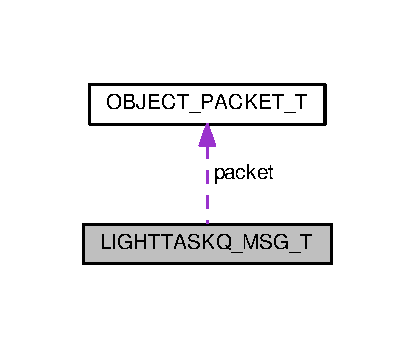
\includegraphics[width=199pt]{structLIGHTTASKQ__MSG__T__coll__graph}
\end{center}
\end{figure}
\subsection*{Data Fields}
\begin{DoxyCompactItemize}
\item 
L\+I\+G\+H\+T\+T\+A\+S\+K\+Q\+\_\+\+M\+S\+G\+I\+D\+\_\+T {\bfseries msg\+ID}\hypertarget{structLIGHTTASKQ__MSG__T_a6d0d6fad55adda1f3922616bc34a7902}{}\label{structLIGHTTASKQ__MSG__T_a6d0d6fad55adda1f3922616bc34a7902}

\item 
T\+A\+S\+K\+\_\+\+I\+D\+E\+N\+T\+I\+F\+I\+E\+R\+\_\+T {\bfseries source\+ID}\hypertarget{structLIGHTTASKQ__MSG__T_a73522367ea6c6c3c9a3e98a817d4c50f}{}\label{structLIGHTTASKQ__MSG__T_a73522367ea6c6c3c9a3e98a817d4c50f}

\item 
\hyperlink{structOBJECT__PACKET__T}{O\+B\+J\+E\+C\+T\+\_\+\+P\+A\+C\+K\+E\+T\+\_\+T} {\bfseries packet}\hypertarget{structLIGHTTASKQ__MSG__T_a9ab5b74f39c56fe79cabf08e00bcd339}{}\label{structLIGHTTASKQ__MSG__T_a9ab5b74f39c56fe79cabf08e00bcd339}

\end{DoxyCompactItemize}


The documentation for this struct was generated from the following file\+:\begin{DoxyCompactItemize}
\item 
/home/gunj/repos/\+E\+C\+E\+N-\/5013/\+Project1/include/common/\hyperlink{light__sensor__task_8h}{light\+\_\+sensor\+\_\+task.\+h}\end{DoxyCompactItemize}

\hypertarget{structLOGGERTASKQ__MSG__T}{}\section{L\+O\+G\+G\+E\+R\+T\+A\+S\+K\+Q\+\_\+\+M\+S\+G\+\_\+T Struct Reference}
\label{structLOGGERTASKQ__MSG__T}\index{L\+O\+G\+G\+E\+R\+T\+A\+S\+K\+Q\+\_\+\+M\+S\+G\+\_\+T@{L\+O\+G\+G\+E\+R\+T\+A\+S\+K\+Q\+\_\+\+M\+S\+G\+\_\+T}}
\subsection*{Data Fields}
\begin{DoxyCompactItemize}
\item 
L\+O\+G\+G\+E\+R\+T\+A\+S\+K\+Q\+\_\+\+M\+S\+G\+I\+D\+\_\+T {\bfseries msg\+ID}\hypertarget{structLOGGERTASKQ__MSG__T_a6f3f926915ee4fed9eefaa2ae02565a0}{}\label{structLOGGERTASKQ__MSG__T_a6f3f926915ee4fed9eefaa2ae02565a0}

\item 
char {\bfseries timestamp} \mbox{[}20\mbox{]}\hypertarget{structLOGGERTASKQ__MSG__T_ad92d934c36ea8b693e20bd585b12dd36}{}\label{structLOGGERTASKQ__MSG__T_ad92d934c36ea8b693e20bd585b12dd36}

\item 
L\+O\+G\+\_\+\+L\+E\+V\+E\+L\+\_\+T {\bfseries loglevel}\hypertarget{structLOGGERTASKQ__MSG__T_abe7f4a15b1008087838d78abe25fd9d1}{}\label{structLOGGERTASKQ__MSG__T_abe7f4a15b1008087838d78abe25fd9d1}

\item 
T\+A\+S\+K\+\_\+\+I\+D\+E\+N\+T\+I\+F\+I\+E\+R\+\_\+T {\bfseries source\+ID}\hypertarget{structLOGGERTASKQ__MSG__T_a4bbfcb4a9e1a7846b56410dc69926b92}{}\label{structLOGGERTASKQ__MSG__T_a4bbfcb4a9e1a7846b56410dc69926b92}

\item 
L\+O\+G\+G\+E\+R\+\_\+\+T\+A\+S\+K\+\_\+\+M\+S\+G\+D\+A\+T\+A\+\_\+T {\bfseries msg\+Data} \mbox{[}L\+T\+\_\+\+M\+S\+G\+\_\+\+S\+I\+ZE\mbox{]}\hypertarget{structLOGGERTASKQ__MSG__T_a3105fa742571aeee5d90f15925eded89}{}\label{structLOGGERTASKQ__MSG__T_a3105fa742571aeee5d90f15925eded89}

\end{DoxyCompactItemize}


The documentation for this struct was generated from the following file\+:\begin{DoxyCompactItemize}
\item 
/home/gunj/repos/\+E\+C\+E\+N-\/5013/\+Project1/include/common/\hyperlink{logger__task_8h}{logger\+\_\+task.\+h}\end{DoxyCompactItemize}

\hypertarget{structMAINTASKQ__MSG__T}{}\section{M\+A\+I\+N\+T\+A\+S\+K\+Q\+\_\+\+M\+S\+G\+\_\+T Struct Reference}
\label{structMAINTASKQ__MSG__T}\index{M\+A\+I\+N\+T\+A\+S\+K\+Q\+\_\+\+M\+S\+G\+\_\+T@{M\+A\+I\+N\+T\+A\+S\+K\+Q\+\_\+\+M\+S\+G\+\_\+T}}
\subsection*{Data Fields}
\begin{DoxyCompactItemize}
\item 
M\+A\+I\+N\+T\+A\+S\+K\+Q\+\_\+\+M\+S\+G\+I\+D\+\_\+T {\bfseries msg\+ID}\hypertarget{structMAINTASKQ__MSG__T_a42b4bf212bc5f1e3cff97ca900552c0e}{}\label{structMAINTASKQ__MSG__T_a42b4bf212bc5f1e3cff97ca900552c0e}

\item 
T\+A\+S\+K\+\_\+\+I\+D\+E\+N\+T\+I\+F\+I\+E\+R\+\_\+T {\bfseries source\+ID}\hypertarget{structMAINTASKQ__MSG__T_a5bbb761b7478733f356d9fe742f47f47}{}\label{structMAINTASKQ__MSG__T_a5bbb761b7478733f356d9fe742f47f47}

\item 
M\+A\+I\+N\+T\+\_\+\+T\+A\+S\+K\+\_\+\+M\+S\+G\+D\+A\+T\+A\+\_\+T {\bfseries msg\+Data} \mbox{[}M\+T\+\_\+\+M\+S\+G\+\_\+\+S\+I\+ZE\mbox{]}\hypertarget{structMAINTASKQ__MSG__T_a0bdf6667da37ec4eff16226085889fcd}{}\label{structMAINTASKQ__MSG__T_a0bdf6667da37ec4eff16226085889fcd}

\end{DoxyCompactItemize}


The documentation for this struct was generated from the following file\+:\begin{DoxyCompactItemize}
\item 
/home/gunj/repos/\+E\+C\+E\+N-\/5013/\+Project1/include/common/\hyperlink{main__task_8h}{main\+\_\+task.\+h}\end{DoxyCompactItemize}

\hypertarget{structOBJECT__PACKET__T}{}\section{O\+B\+J\+E\+C\+T\+\_\+\+P\+A\+C\+K\+E\+T\+\_\+T Struct Reference}
\label{structOBJECT__PACKET__T}\index{O\+B\+J\+E\+C\+T\+\_\+\+P\+A\+C\+K\+E\+T\+\_\+T@{O\+B\+J\+E\+C\+T\+\_\+\+P\+A\+C\+K\+E\+T\+\_\+T}}
\subsection*{Data Fields}
\begin{DoxyCompactItemize}
\item 
S\+Y\+N\+C\+\_\+\+T\+Y\+P\+E\+\_\+T {\bfseries is\+\_\+sync}\hypertarget{structOBJECT__PACKET__T_a1648380d5d2dd74ec2e13957949e505e}{}\label{structOBJECT__PACKET__T_a1648380d5d2dd74ec2e13957949e505e}

\item 
sem\+\_\+t $\ast$ {\bfseries sync\+\_\+semaphore}\hypertarget{structOBJECT__PACKET__T_a13b703828ad6478fbffdb99e3c24941c}{}\label{structOBJECT__PACKET__T_a13b703828ad6478fbffdb99e3c24941c}

\item 
D\+E\+V\+\_\+\+R\+E\+G\+\_\+T {\bfseries dev\+\_\+addr}\hypertarget{structOBJECT__PACKET__T_a7b42c85d01c47b432bbd8a86d80b1881}{}\label{structOBJECT__PACKET__T_a7b42c85d01c47b432bbd8a86d80b1881}

\item 
P\+\_\+\+B\+U\+F\+F\+\_\+T $\ast$ {\bfseries reg\+\_\+value}\hypertarget{structOBJECT__PACKET__T_a927d74894329c73aa0a192f110d47671}{}\label{structOBJECT__PACKET__T_a927d74894329c73aa0a192f110d47671}

\item 
B\+U\+F\+F\+\_\+\+L\+E\+N\+\_\+T {\bfseries buff\+Len}\hypertarget{structOBJECT__PACKET__T_a1f397ae898402a439fc093c5347459ae}{}\label{structOBJECT__PACKET__T_a1f397ae898402a439fc093c5347459ae}

\end{DoxyCompactItemize}


The documentation for this struct was generated from the following file\+:\begin{DoxyCompactItemize}
\item 
/home/gunj/repos/\+E\+C\+E\+N-\/5013/\+Project1/include/common/\hyperlink{sensor__common__object_8h}{sensor\+\_\+common\+\_\+object.\+h}\end{DoxyCompactItemize}

\hypertarget{structREMOTE__REQUEST__T}{}\section{R\+E\+M\+O\+T\+E\+\_\+\+R\+E\+Q\+U\+E\+S\+T\+\_\+T Struct Reference}
\label{structREMOTE__REQUEST__T}\index{R\+E\+M\+O\+T\+E\+\_\+\+R\+E\+Q\+U\+E\+S\+T\+\_\+T@{R\+E\+M\+O\+T\+E\+\_\+\+R\+E\+Q\+U\+E\+S\+T\+\_\+T}}
\subsection*{Data Fields}
\begin{DoxyCompactItemize}
\item 
R\+E\+M\+O\+T\+E\+\_\+\+R\+E\+Q\+R\+S\+P\+\_\+\+ID {\bfseries request\+\_\+id}\hypertarget{structREMOTE__REQUEST__T_aa9abf86717ba38441b7620ce1a435379}{}\label{structREMOTE__REQUEST__T_aa9abf86717ba38441b7620ce1a435379}

\end{DoxyCompactItemize}


The documentation for this struct was generated from the following file\+:\begin{DoxyCompactItemize}
\item 
/home/gunj/repos/\+E\+C\+E\+N-\/5013/\+Project1/include/common/\hyperlink{sensor__common__object_8h}{sensor\+\_\+common\+\_\+object.\+h}\end{DoxyCompactItemize}

\hypertarget{structREMOTE__RESPONSE__T}{}\section{R\+E\+M\+O\+T\+E\+\_\+\+R\+E\+S\+P\+O\+N\+S\+E\+\_\+T Struct Reference}
\label{structREMOTE__RESPONSE__T}\index{R\+E\+M\+O\+T\+E\+\_\+\+R\+E\+S\+P\+O\+N\+S\+E\+\_\+T@{R\+E\+M\+O\+T\+E\+\_\+\+R\+E\+S\+P\+O\+N\+S\+E\+\_\+T}}


Collaboration diagram for R\+E\+M\+O\+T\+E\+\_\+\+R\+E\+S\+P\+O\+N\+S\+E\+\_\+T\+:\nopagebreak
\begin{figure}[H]
\begin{center}
\leavevmode
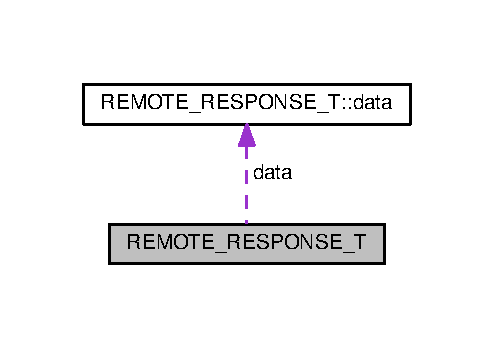
\includegraphics[width=237pt]{structREMOTE__RESPONSE__T__coll__graph}
\end{center}
\end{figure}
\subsection*{Data Structures}
\begin{DoxyCompactItemize}
\item 
union \hyperlink{unionREMOTE__RESPONSE__T_1_1data}{data}
\end{DoxyCompactItemize}
\subsection*{Data Fields}
\begin{DoxyCompactItemize}
\item 
R\+E\+M\+O\+T\+E\+\_\+\+R\+E\+Q\+R\+S\+P\+\_\+\+ID {\bfseries rsp\+\_\+id}\hypertarget{structREMOTE__RESPONSE__T_aeffb937926ea1d5ae378d59eec691357}{}\label{structREMOTE__RESPONSE__T_aeffb937926ea1d5ae378d59eec691357}

\item 
union \hyperlink{unionREMOTE__RESPONSE__T_1_1data}{R\+E\+M\+O\+T\+E\+\_\+\+R\+E\+S\+P\+O\+N\+S\+E\+\_\+\+T\+::data} {\bfseries data}\hypertarget{structREMOTE__RESPONSE__T_a7cf162cedf8f984c2f287815632fdfd0}{}\label{structREMOTE__RESPONSE__T_a7cf162cedf8f984c2f287815632fdfd0}

\item 
char {\bfseries metadata} \mbox{[}20\mbox{]}\hypertarget{structREMOTE__RESPONSE__T_a3382443efefd8a97a65e01578dfa9246}{}\label{structREMOTE__RESPONSE__T_a3382443efefd8a97a65e01578dfa9246}

\end{DoxyCompactItemize}


The documentation for this struct was generated from the following file\+:\begin{DoxyCompactItemize}
\item 
/home/gunj/repos/\+E\+C\+E\+N-\/5013/\+Project1/include/common/\hyperlink{sensor__common__object_8h}{sensor\+\_\+common\+\_\+object.\+h}\end{DoxyCompactItemize}

\hypertarget{structTEMPERATURETASKQ__MSG__T}{}\section{T\+E\+M\+P\+E\+R\+A\+T\+U\+R\+E\+T\+A\+S\+K\+Q\+\_\+\+M\+S\+G\+\_\+T Struct Reference}
\label{structTEMPERATURETASKQ__MSG__T}\index{T\+E\+M\+P\+E\+R\+A\+T\+U\+R\+E\+T\+A\+S\+K\+Q\+\_\+\+M\+S\+G\+\_\+T@{T\+E\+M\+P\+E\+R\+A\+T\+U\+R\+E\+T\+A\+S\+K\+Q\+\_\+\+M\+S\+G\+\_\+T}}


Collaboration diagram for T\+E\+M\+P\+E\+R\+A\+T\+U\+R\+E\+T\+A\+S\+K\+Q\+\_\+\+M\+S\+G\+\_\+T\+:\nopagebreak
\begin{figure}[H]
\begin{center}
\leavevmode
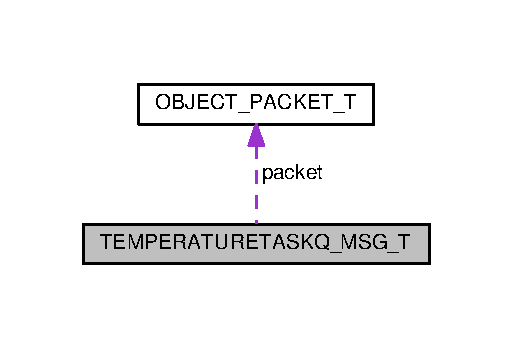
\includegraphics[width=246pt]{structTEMPERATURETASKQ__MSG__T__coll__graph}
\end{center}
\end{figure}
\subsection*{Data Fields}
\begin{DoxyCompactItemize}
\item 
T\+E\+M\+P\+E\+R\+A\+T\+U\+R\+E\+T\+A\+S\+K\+Q\+\_\+\+M\+S\+G\+I\+D\+\_\+T {\bfseries msg\+ID}\hypertarget{structTEMPERATURETASKQ__MSG__T_a3193f82c175e24995eae8c2819c410e3}{}\label{structTEMPERATURETASKQ__MSG__T_a3193f82c175e24995eae8c2819c410e3}

\item 
T\+A\+S\+K\+\_\+\+I\+D\+E\+N\+T\+I\+F\+I\+E\+R\+\_\+T {\bfseries source\+ID}\hypertarget{structTEMPERATURETASKQ__MSG__T_ae8775f7bc7322da94b6827c42f28ffd1}{}\label{structTEMPERATURETASKQ__MSG__T_ae8775f7bc7322da94b6827c42f28ffd1}

\item 
\hyperlink{structOBJECT__PACKET__T}{O\+B\+J\+E\+C\+T\+\_\+\+P\+A\+C\+K\+E\+T\+\_\+T} {\bfseries packet}\hypertarget{structTEMPERATURETASKQ__MSG__T_ad8ac382a5319e5252b1af86b45333fb8}{}\label{structTEMPERATURETASKQ__MSG__T_ad8ac382a5319e5252b1af86b45333fb8}

\end{DoxyCompactItemize}


The documentation for this struct was generated from the following file\+:\begin{DoxyCompactItemize}
\item 
/home/gunj/repos/\+E\+C\+E\+N-\/5013/\+Project1/include/common/\hyperlink{temperature__sensor__task_8h}{temperature\+\_\+sensor\+\_\+task.\+h}\end{DoxyCompactItemize}

\hypertarget{structTMP102__CONFIG__REG__SETTINGS__T}{}\section{T\+M\+P102\+\_\+\+C\+O\+N\+F\+I\+G\+\_\+\+R\+E\+G\+\_\+\+S\+E\+T\+T\+I\+N\+G\+S\+\_\+T Struct Reference}
\label{structTMP102__CONFIG__REG__SETTINGS__T}\index{T\+M\+P102\+\_\+\+C\+O\+N\+F\+I\+G\+\_\+\+R\+E\+G\+\_\+\+S\+E\+T\+T\+I\+N\+G\+S\+\_\+T@{T\+M\+P102\+\_\+\+C\+O\+N\+F\+I\+G\+\_\+\+R\+E\+G\+\_\+\+S\+E\+T\+T\+I\+N\+G\+S\+\_\+T}}
\subsection*{Data Fields}
\begin{DoxyCompactItemize}
\item 
uint16\+\_\+t \hyperlink{structTMP102__CONFIG__REG__SETTINGS__T_a81f77be9673afe30da33edb8e6e62b55}{S\+D\+\_\+\+M\+O\+DE}\+:1
\item 
uint16\+\_\+t \hyperlink{structTMP102__CONFIG__REG__SETTINGS__T_a635d77b82a949a2299e1981d7ace305d}{T\+M\+\_\+\+M\+O\+DE}\+:1
\item 
uint16\+\_\+t \hyperlink{structTMP102__CONFIG__REG__SETTINGS__T_a2225a8d1e41436fe30577b474c99c737}{P\+OL}\+:1
\item 
uint16\+\_\+t \hyperlink{structTMP102__CONFIG__REG__SETTINGS__T_a6c73d5cc6105f5afd1dbb33454705ec3}{F\+A\+U\+LT}\+:2
\item 
const uint16\+\_\+t {\bfseries R\+E\+S0}\+:2\hypertarget{structTMP102__CONFIG__REG__SETTINGS__T_ae0c076ab9ff772db54bd811ecf1cef71}{}\label{structTMP102__CONFIG__REG__SETTINGS__T_ae0c076ab9ff772db54bd811ecf1cef71}

\item 
uint16\+\_\+t \hyperlink{structTMP102__CONFIG__REG__SETTINGS__T_a09870f580e0e800f3eb23f640f07a3c3}{OS}\+:1
\item 
const uint16\+\_\+t {\bfseries R\+E\+S1}\+:4\hypertarget{structTMP102__CONFIG__REG__SETTINGS__T_a62bc2c4b934d561e2f32949c61f6b016}{}\label{structTMP102__CONFIG__REG__SETTINGS__T_a62bc2c4b934d561e2f32949c61f6b016}

\item 
uint16\+\_\+t \hyperlink{structTMP102__CONFIG__REG__SETTINGS__T_a9837531af532e0c8a1fdd39095c250fb}{E\+M\+\_\+\+M\+O\+DE}\+:1
\item 
const uint16\+\_\+t \hyperlink{structTMP102__CONFIG__REG__SETTINGS__T_a7bd3f8bf4d72156773a9cb9abde52596}{R\+O\+\_\+\+A\+L\+\_\+\+M\+O\+DE}\+:1
\item 
uint16\+\_\+t \hyperlink{structTMP102__CONFIG__REG__SETTINGS__T_aa0d2ccdd3d62d5f817bd34be36ddb2b1}{CR}\+:2
\end{DoxyCompactItemize}


\subsection{Field Documentation}
\index{T\+M\+P102\+\_\+\+C\+O\+N\+F\+I\+G\+\_\+\+R\+E\+G\+\_\+\+S\+E\+T\+T\+I\+N\+G\+S\+\_\+T@{T\+M\+P102\+\_\+\+C\+O\+N\+F\+I\+G\+\_\+\+R\+E\+G\+\_\+\+S\+E\+T\+T\+I\+N\+G\+S\+\_\+T}!CR@{CR}}
\index{CR@{CR}!T\+M\+P102\+\_\+\+C\+O\+N\+F\+I\+G\+\_\+\+R\+E\+G\+\_\+\+S\+E\+T\+T\+I\+N\+G\+S\+\_\+T@{T\+M\+P102\+\_\+\+C\+O\+N\+F\+I\+G\+\_\+\+R\+E\+G\+\_\+\+S\+E\+T\+T\+I\+N\+G\+S\+\_\+T}}
\subsubsection[{\texorpdfstring{CR}{CR}}]{\setlength{\rightskip}{0pt plus 5cm}uint16\+\_\+t T\+M\+P102\+\_\+\+C\+O\+N\+F\+I\+G\+\_\+\+R\+E\+G\+\_\+\+S\+E\+T\+T\+I\+N\+G\+S\+\_\+\+T\+::\+CR}\hypertarget{structTMP102__CONFIG__REG__SETTINGS__T_aa0d2ccdd3d62d5f817bd34be36ddb2b1}{}\label{structTMP102__CONFIG__REG__SETTINGS__T_aa0d2ccdd3d62d5f817bd34be36ddb2b1}

\begin{DoxyItemize}
\item 0 = 0.\+25\+Hz ; 1 = 1\+Hz ; (D)2 = 4\+Hz ; 3 = 8\+Hz $\ast$/ 
\end{DoxyItemize}\index{T\+M\+P102\+\_\+\+C\+O\+N\+F\+I\+G\+\_\+\+R\+E\+G\+\_\+\+S\+E\+T\+T\+I\+N\+G\+S\+\_\+T@{T\+M\+P102\+\_\+\+C\+O\+N\+F\+I\+G\+\_\+\+R\+E\+G\+\_\+\+S\+E\+T\+T\+I\+N\+G\+S\+\_\+T}!E\+M\+\_\+\+M\+O\+DE@{E\+M\+\_\+\+M\+O\+DE}}
\index{E\+M\+\_\+\+M\+O\+DE@{E\+M\+\_\+\+M\+O\+DE}!T\+M\+P102\+\_\+\+C\+O\+N\+F\+I\+G\+\_\+\+R\+E\+G\+\_\+\+S\+E\+T\+T\+I\+N\+G\+S\+\_\+T@{T\+M\+P102\+\_\+\+C\+O\+N\+F\+I\+G\+\_\+\+R\+E\+G\+\_\+\+S\+E\+T\+T\+I\+N\+G\+S\+\_\+T}}
\subsubsection[{\texorpdfstring{E\+M\+\_\+\+M\+O\+DE}{EM_MODE}}]{\setlength{\rightskip}{0pt plus 5cm}uint16\+\_\+t T\+M\+P102\+\_\+\+C\+O\+N\+F\+I\+G\+\_\+\+R\+E\+G\+\_\+\+S\+E\+T\+T\+I\+N\+G\+S\+\_\+\+T\+::\+E\+M\+\_\+\+M\+O\+DE}\hypertarget{structTMP102__CONFIG__REG__SETTINGS__T_a9837531af532e0c8a1fdd39095c250fb}{}\label{structTMP102__CONFIG__REG__SETTINGS__T_a9837531af532e0c8a1fdd39095c250fb}

\begin{DoxyItemize}
\item (D)0 = Normal mode(12bit); 1= Extended mode(13 bit) $\ast$/ 
\end{DoxyItemize}\index{T\+M\+P102\+\_\+\+C\+O\+N\+F\+I\+G\+\_\+\+R\+E\+G\+\_\+\+S\+E\+T\+T\+I\+N\+G\+S\+\_\+T@{T\+M\+P102\+\_\+\+C\+O\+N\+F\+I\+G\+\_\+\+R\+E\+G\+\_\+\+S\+E\+T\+T\+I\+N\+G\+S\+\_\+T}!F\+A\+U\+LT@{F\+A\+U\+LT}}
\index{F\+A\+U\+LT@{F\+A\+U\+LT}!T\+M\+P102\+\_\+\+C\+O\+N\+F\+I\+G\+\_\+\+R\+E\+G\+\_\+\+S\+E\+T\+T\+I\+N\+G\+S\+\_\+T@{T\+M\+P102\+\_\+\+C\+O\+N\+F\+I\+G\+\_\+\+R\+E\+G\+\_\+\+S\+E\+T\+T\+I\+N\+G\+S\+\_\+T}}
\subsubsection[{\texorpdfstring{F\+A\+U\+LT}{FAULT}}]{\setlength{\rightskip}{0pt plus 5cm}uint16\+\_\+t T\+M\+P102\+\_\+\+C\+O\+N\+F\+I\+G\+\_\+\+R\+E\+G\+\_\+\+S\+E\+T\+T\+I\+N\+G\+S\+\_\+\+T\+::\+F\+A\+U\+LT}\hypertarget{structTMP102__CONFIG__REG__SETTINGS__T_a6c73d5cc6105f5afd1dbb33454705ec3}{}\label{structTMP102__CONFIG__REG__SETTINGS__T_a6c73d5cc6105f5afd1dbb33454705ec3}

\begin{DoxyItemize}
\item (D)0 = 1\+Fault; 1= 2\+Faults; 3 = 4\+Faults; 4=6\+Faults $\ast$/ 
\end{DoxyItemize}\index{T\+M\+P102\+\_\+\+C\+O\+N\+F\+I\+G\+\_\+\+R\+E\+G\+\_\+\+S\+E\+T\+T\+I\+N\+G\+S\+\_\+T@{T\+M\+P102\+\_\+\+C\+O\+N\+F\+I\+G\+\_\+\+R\+E\+G\+\_\+\+S\+E\+T\+T\+I\+N\+G\+S\+\_\+T}!OS@{OS}}
\index{OS@{OS}!T\+M\+P102\+\_\+\+C\+O\+N\+F\+I\+G\+\_\+\+R\+E\+G\+\_\+\+S\+E\+T\+T\+I\+N\+G\+S\+\_\+T@{T\+M\+P102\+\_\+\+C\+O\+N\+F\+I\+G\+\_\+\+R\+E\+G\+\_\+\+S\+E\+T\+T\+I\+N\+G\+S\+\_\+T}}
\subsubsection[{\texorpdfstring{OS}{OS}}]{\setlength{\rightskip}{0pt plus 5cm}uint16\+\_\+t T\+M\+P102\+\_\+\+C\+O\+N\+F\+I\+G\+\_\+\+R\+E\+G\+\_\+\+S\+E\+T\+T\+I\+N\+G\+S\+\_\+\+T\+::\+OS}\hypertarget{structTMP102__CONFIG__REG__SETTINGS__T_a09870f580e0e800f3eb23f640f07a3c3}{}\label{structTMP102__CONFIG__REG__SETTINGS__T_a09870f580e0e800f3eb23f640f07a3c3}

\begin{DoxyItemize}
\item (D)0 = During the conversion, the OS bit reads \textquotesingle{}0\textquotesingle{}; 1 = writing a 1 to the OS bit starts a single temperature conversion $\ast$/ 
\end{DoxyItemize}\index{T\+M\+P102\+\_\+\+C\+O\+N\+F\+I\+G\+\_\+\+R\+E\+G\+\_\+\+S\+E\+T\+T\+I\+N\+G\+S\+\_\+T@{T\+M\+P102\+\_\+\+C\+O\+N\+F\+I\+G\+\_\+\+R\+E\+G\+\_\+\+S\+E\+T\+T\+I\+N\+G\+S\+\_\+T}!P\+OL@{P\+OL}}
\index{P\+OL@{P\+OL}!T\+M\+P102\+\_\+\+C\+O\+N\+F\+I\+G\+\_\+\+R\+E\+G\+\_\+\+S\+E\+T\+T\+I\+N\+G\+S\+\_\+T@{T\+M\+P102\+\_\+\+C\+O\+N\+F\+I\+G\+\_\+\+R\+E\+G\+\_\+\+S\+E\+T\+T\+I\+N\+G\+S\+\_\+T}}
\subsubsection[{\texorpdfstring{P\+OL}{POL}}]{\setlength{\rightskip}{0pt plus 5cm}uint16\+\_\+t T\+M\+P102\+\_\+\+C\+O\+N\+F\+I\+G\+\_\+\+R\+E\+G\+\_\+\+S\+E\+T\+T\+I\+N\+G\+S\+\_\+\+T\+::\+P\+OL}\hypertarget{structTMP102__CONFIG__REG__SETTINGS__T_a2225a8d1e41436fe30577b474c99c737}{}\label{structTMP102__CONFIG__REG__SETTINGS__T_a2225a8d1e41436fe30577b474c99c737}

\begin{DoxyItemize}
\item (D)0 = A\+L\+E\+RT pin becomes active low; 1 = A\+L\+E\+RT pin becomes active high and the state of the A\+L\+E\+RT pin is inverted. $\ast$/ 
\end{DoxyItemize}\index{T\+M\+P102\+\_\+\+C\+O\+N\+F\+I\+G\+\_\+\+R\+E\+G\+\_\+\+S\+E\+T\+T\+I\+N\+G\+S\+\_\+T@{T\+M\+P102\+\_\+\+C\+O\+N\+F\+I\+G\+\_\+\+R\+E\+G\+\_\+\+S\+E\+T\+T\+I\+N\+G\+S\+\_\+T}!R\+O\+\_\+\+A\+L\+\_\+\+M\+O\+DE@{R\+O\+\_\+\+A\+L\+\_\+\+M\+O\+DE}}
\index{R\+O\+\_\+\+A\+L\+\_\+\+M\+O\+DE@{R\+O\+\_\+\+A\+L\+\_\+\+M\+O\+DE}!T\+M\+P102\+\_\+\+C\+O\+N\+F\+I\+G\+\_\+\+R\+E\+G\+\_\+\+S\+E\+T\+T\+I\+N\+G\+S\+\_\+T@{T\+M\+P102\+\_\+\+C\+O\+N\+F\+I\+G\+\_\+\+R\+E\+G\+\_\+\+S\+E\+T\+T\+I\+N\+G\+S\+\_\+T}}
\subsubsection[{\texorpdfstring{R\+O\+\_\+\+A\+L\+\_\+\+M\+O\+DE}{RO_AL_MODE}}]{\setlength{\rightskip}{0pt plus 5cm}const uint16\+\_\+t T\+M\+P102\+\_\+\+C\+O\+N\+F\+I\+G\+\_\+\+R\+E\+G\+\_\+\+S\+E\+T\+T\+I\+N\+G\+S\+\_\+\+T\+::\+R\+O\+\_\+\+A\+L\+\_\+\+M\+O\+DE}\hypertarget{structTMP102__CONFIG__REG__SETTINGS__T_a7bd3f8bf4d72156773a9cb9abde52596}{}\label{structTMP102__CONFIG__REG__SETTINGS__T_a7bd3f8bf4d72156773a9cb9abde52596}

\begin{DoxyItemize}
\item Reads the AL bit$\ast$/ 
\end{DoxyItemize}\index{T\+M\+P102\+\_\+\+C\+O\+N\+F\+I\+G\+\_\+\+R\+E\+G\+\_\+\+S\+E\+T\+T\+I\+N\+G\+S\+\_\+T@{T\+M\+P102\+\_\+\+C\+O\+N\+F\+I\+G\+\_\+\+R\+E\+G\+\_\+\+S\+E\+T\+T\+I\+N\+G\+S\+\_\+T}!S\+D\+\_\+\+M\+O\+DE@{S\+D\+\_\+\+M\+O\+DE}}
\index{S\+D\+\_\+\+M\+O\+DE@{S\+D\+\_\+\+M\+O\+DE}!T\+M\+P102\+\_\+\+C\+O\+N\+F\+I\+G\+\_\+\+R\+E\+G\+\_\+\+S\+E\+T\+T\+I\+N\+G\+S\+\_\+T@{T\+M\+P102\+\_\+\+C\+O\+N\+F\+I\+G\+\_\+\+R\+E\+G\+\_\+\+S\+E\+T\+T\+I\+N\+G\+S\+\_\+T}}
\subsubsection[{\texorpdfstring{S\+D\+\_\+\+M\+O\+DE}{SD_MODE}}]{\setlength{\rightskip}{0pt plus 5cm}uint16\+\_\+t T\+M\+P102\+\_\+\+C\+O\+N\+F\+I\+G\+\_\+\+R\+E\+G\+\_\+\+S\+E\+T\+T\+I\+N\+G\+S\+\_\+\+T\+::\+S\+D\+\_\+\+M\+O\+DE}\hypertarget{structTMP102__CONFIG__REG__SETTINGS__T_a81f77be9673afe30da33edb8e6e62b55}{}\label{structTMP102__CONFIG__REG__SETTINGS__T_a81f77be9673afe30da33edb8e6e62b55}

\begin{DoxyItemize}
\item (D)0 = Continuous conversion; 1 = Can sleep$\ast$/ 
\end{DoxyItemize}\index{T\+M\+P102\+\_\+\+C\+O\+N\+F\+I\+G\+\_\+\+R\+E\+G\+\_\+\+S\+E\+T\+T\+I\+N\+G\+S\+\_\+T@{T\+M\+P102\+\_\+\+C\+O\+N\+F\+I\+G\+\_\+\+R\+E\+G\+\_\+\+S\+E\+T\+T\+I\+N\+G\+S\+\_\+T}!T\+M\+\_\+\+M\+O\+DE@{T\+M\+\_\+\+M\+O\+DE}}
\index{T\+M\+\_\+\+M\+O\+DE@{T\+M\+\_\+\+M\+O\+DE}!T\+M\+P102\+\_\+\+C\+O\+N\+F\+I\+G\+\_\+\+R\+E\+G\+\_\+\+S\+E\+T\+T\+I\+N\+G\+S\+\_\+T@{T\+M\+P102\+\_\+\+C\+O\+N\+F\+I\+G\+\_\+\+R\+E\+G\+\_\+\+S\+E\+T\+T\+I\+N\+G\+S\+\_\+T}}
\subsubsection[{\texorpdfstring{T\+M\+\_\+\+M\+O\+DE}{TM_MODE}}]{\setlength{\rightskip}{0pt plus 5cm}uint16\+\_\+t T\+M\+P102\+\_\+\+C\+O\+N\+F\+I\+G\+\_\+\+R\+E\+G\+\_\+\+S\+E\+T\+T\+I\+N\+G\+S\+\_\+\+T\+::\+T\+M\+\_\+\+M\+O\+DE}\hypertarget{structTMP102__CONFIG__REG__SETTINGS__T_a635d77b82a949a2299e1981d7ace305d}{}\label{structTMP102__CONFIG__REG__SETTINGS__T_a635d77b82a949a2299e1981d7ace305d}

\begin{DoxyItemize}
\item (D)0 = Comparatore mode; 1 = Interrupt mode$\ast$/ 
\end{DoxyItemize}

The documentation for this struct was generated from the following file\+:\begin{DoxyCompactItemize}
\item 
/home/gunj/repos/\+E\+C\+E\+N-\/5013/\+Project1/include/\+Beagle\+Bone/\hyperlink{tmp102__sensor_8h}{tmp102\+\_\+sensor.\+h}\end{DoxyCompactItemize}

\chapter{File Documentation}
\hypertarget{apds9301__sensor_8h}{}\section{/home/gunj/repos/\+E\+C\+E\+N-\/5013/\+Project1/include/\+Beagle\+Bone/apds9301\+\_\+sensor.h File Reference}
\label{apds9301__sensor_8h}\index{/home/gunj/repos/\+E\+C\+E\+N-\/5013/\+Project1/include/\+Beagle\+Bone/apds9301\+\_\+sensor.\+h@{/home/gunj/repos/\+E\+C\+E\+N-\/5013/\+Project1/include/\+Beagle\+Bone/apds9301\+\_\+sensor.\+h}}
{\ttfamily \#include $<$stdint.\+h$>$}\\*
Include dependency graph for apds9301\+\_\+sensor.\+h\+:\nopagebreak
\begin{figure}[H]
\begin{center}
\leavevmode
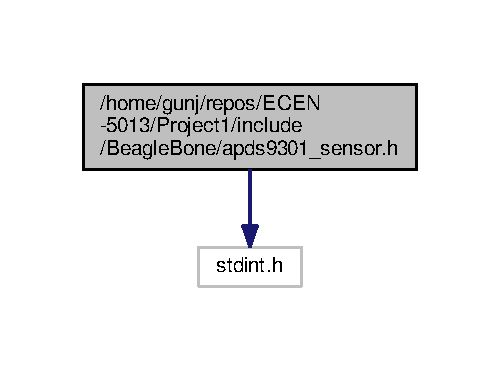
\includegraphics[width=240pt]{apds9301__sensor_8h__incl}
\end{center}
\end{figure}
This graph shows which files directly or indirectly include this file\+:\nopagebreak
\begin{figure}[H]
\begin{center}
\leavevmode
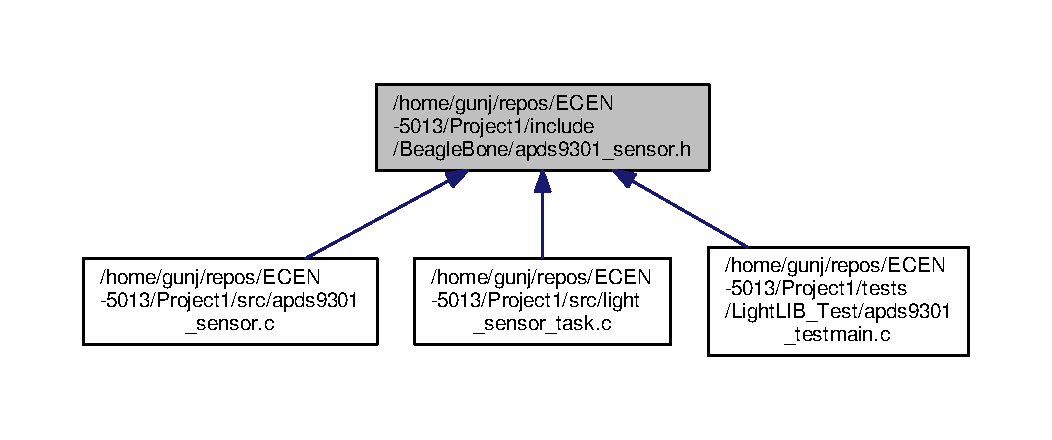
\includegraphics[width=350pt]{apds9301__sensor_8h__dep__incl}
\end{center}
\end{figure}
\subsection*{Macros}
\begin{DoxyCompactItemize}
\item 
\#define {\bfseries A\+P\+D\+S9301\+\_\+\+S\+L\+A\+V\+E\+\_\+\+A\+D\+DR}~(0x39)\hypertarget{apds9301__sensor_8h_aa45ac33ec93739717b49de5343f7f05c}{}\label{apds9301__sensor_8h_aa45ac33ec93739717b49de5343f7f05c}

\item 
\#define {\bfseries A\+P\+D\+S9301\+\_\+\+C\+M\+D\+\_\+\+R\+EG}~(0x80)\hypertarget{apds9301__sensor_8h_aa8cbe8551313b2f06715d25f0b6c6468}{}\label{apds9301__sensor_8h_aa8cbe8551313b2f06715d25f0b6c6468}

\item 
\#define {\bfseries A\+P\+D\+S9301\+\_\+\+C\+M\+D\+\_\+\+W\+O\+R\+D\+\_\+\+EN}~(1$<$$<$5)\hypertarget{apds9301__sensor_8h_ac95a6add6403cbf8552ff1cbc6f98d2a}{}\label{apds9301__sensor_8h_ac95a6add6403cbf8552ff1cbc6f98d2a}

\item 
\#define {\bfseries A\+P\+D\+S9301\+\_\+\+C\+M\+D\+\_\+\+I\+N\+T\+\_\+\+C\+L\+E\+AR}~(1$<$6)\hypertarget{apds9301__sensor_8h_a37a0f41c63f37ab143b7263867199fd8}{}\label{apds9301__sensor_8h_a37a0f41c63f37ab143b7263867199fd8}

\item 
\#define {\bfseries A\+P\+D\+S9301\+\_\+\+C\+T\+R\+L\+\_\+\+R\+EG}~(0x00) $\vert$ A\+P\+D\+S9301\+\_\+\+C\+M\+D\+\_\+\+R\+EG\hypertarget{apds9301__sensor_8h_aeb73944a113591006450246b4e00c532}{}\label{apds9301__sensor_8h_aeb73944a113591006450246b4e00c532}

\item 
\#define {\bfseries A\+P\+D\+S9301\+\_\+\+T\+I\+M\+I\+N\+G\+\_\+\+R\+EG}~(0x01) $\vert$ A\+P\+D\+S9301\+\_\+\+C\+M\+D\+\_\+\+R\+EG\hypertarget{apds9301__sensor_8h_ad633b4f59b5c3b8aa0f1e3ff310f6d8b}{}\label{apds9301__sensor_8h_ad633b4f59b5c3b8aa0f1e3ff310f6d8b}

\item 
\#define {\bfseries A\+P\+D\+S9301\+\_\+\+I\+D\+\_\+\+R\+EG}~(0x0\+A) $\vert$ A\+P\+D\+S9301\+\_\+\+C\+M\+D\+\_\+\+R\+EG\hypertarget{apds9301__sensor_8h_a6af905a9f6d4e38491bd03dbde2115ec}{}\label{apds9301__sensor_8h_a6af905a9f6d4e38491bd03dbde2115ec}

\item 
\#define {\bfseries A\+P\+D\+S9301\+\_\+\+I\+N\+T\+\_\+\+C\+T\+R\+L\+\_\+\+R\+EG}~(0x06) $\vert$ A\+P\+D\+S9301\+\_\+\+C\+M\+D\+\_\+\+R\+EG\hypertarget{apds9301__sensor_8h_a4730042ee11dee3cbc7b4b81255b900e}{}\label{apds9301__sensor_8h_a4730042ee11dee3cbc7b4b81255b900e}

\item 
\#define {\bfseries A\+P\+D\+S9301\+\_\+\+C\+H0\+\_\+\+D\+A\+T\+A\+L\+OW}~(0x0\+C) $\vert$ A\+P\+D\+S9301\+\_\+\+C\+M\+D\+\_\+\+R\+EG\hypertarget{apds9301__sensor_8h_acccb3291ba8767dc6bc2922edcef4579}{}\label{apds9301__sensor_8h_acccb3291ba8767dc6bc2922edcef4579}

\item 
\#define {\bfseries A\+P\+D\+S9301\+\_\+\+C\+H0\+\_\+\+D\+A\+T\+A\+H\+I\+GH}~(0x0\+D) $\vert$ A\+P\+D\+S9301\+\_\+\+C\+M\+D\+\_\+\+R\+EG\hypertarget{apds9301__sensor_8h_abf415770e699fa605cf146b790c93bd4}{}\label{apds9301__sensor_8h_abf415770e699fa605cf146b790c93bd4}

\item 
\#define {\bfseries A\+P\+D\+S9301\+\_\+\+C\+H1\+\_\+\+D\+A\+T\+A\+L\+OW}~(0x0\+E) $\vert$ A\+P\+D\+S9301\+\_\+\+C\+M\+D\+\_\+\+R\+EG\hypertarget{apds9301__sensor_8h_a5b84ad3188b098cdff2627ea85e54940}{}\label{apds9301__sensor_8h_a5b84ad3188b098cdff2627ea85e54940}

\item 
\#define {\bfseries A\+P\+D\+S9301\+\_\+\+C\+H1\+\_\+\+D\+A\+T\+A\+H\+I\+GH}~(0x0\+F) $\vert$ A\+P\+D\+S9301\+\_\+\+C\+M\+D\+\_\+\+R\+EG\hypertarget{apds9301__sensor_8h_ad9688e08e3516468dcef1b4eebaf3ed3}{}\label{apds9301__sensor_8h_ad9688e08e3516468dcef1b4eebaf3ed3}

\item 
\#define {\bfseries A\+P\+D\+S9301\+\_\+\+I\+N\+T\+\_\+\+T\+H\+\_\+\+L\+L\+\_\+\+R\+EG}~(0x02) $\vert$ A\+P\+D\+S9301\+\_\+\+C\+M\+D\+\_\+\+R\+EG\hypertarget{apds9301__sensor_8h_a3acf2fb4357537fe9ab495ce47c0fc5c}{}\label{apds9301__sensor_8h_a3acf2fb4357537fe9ab495ce47c0fc5c}

\item 
\#define {\bfseries A\+P\+D\+S9301\+\_\+\+I\+N\+T\+\_\+\+T\+H\+\_\+\+L\+H\+\_\+\+R\+EG}~(0x03) $\vert$ A\+P\+D\+S9301\+\_\+\+C\+M\+D\+\_\+\+R\+EG\hypertarget{apds9301__sensor_8h_a01be36bf3154f6890b784cd88b27e555}{}\label{apds9301__sensor_8h_a01be36bf3154f6890b784cd88b27e555}

\item 
\#define {\bfseries A\+P\+D\+S9301\+\_\+\+I\+N\+T\+\_\+\+T\+H\+\_\+\+H\+L\+\_\+\+R\+EG}~(0x04) $\vert$ A\+P\+D\+S9301\+\_\+\+C\+M\+D\+\_\+\+R\+EG\hypertarget{apds9301__sensor_8h_a2f501fc33fa9cd4f214bd8534e2d74d1}{}\label{apds9301__sensor_8h_a2f501fc33fa9cd4f214bd8534e2d74d1}

\item 
\#define {\bfseries A\+P\+D\+S9301\+\_\+\+I\+N\+T\+\_\+\+T\+H\+\_\+\+H\+H\+\_\+\+R\+EG}~(0x05) $\vert$ A\+P\+D\+S9301\+\_\+\+C\+M\+D\+\_\+\+R\+EG\hypertarget{apds9301__sensor_8h_a5444a0c9d6096969c7b61f53f2fe2ba3}{}\label{apds9301__sensor_8h_a5444a0c9d6096969c7b61f53f2fe2ba3}

\item 
\#define {\bfseries A\+P\+D\+S9301\+\_\+\+C\+T\+R\+L\+\_\+\+P\+O\+W\+E\+R\+ON}~(0x03)\hypertarget{apds9301__sensor_8h_a58ecb82a7e59d10bde67c25919e36318}{}\label{apds9301__sensor_8h_a58ecb82a7e59d10bde67c25919e36318}

\item 
\#define {\bfseries A\+P\+D\+S9301\+\_\+\+C\+T\+R\+L\+\_\+\+P\+O\+W\+E\+R\+O\+FF}~(0x00)\hypertarget{apds9301__sensor_8h_a055ed2e5866eb44e95a42c7eb4d15c0b}{}\label{apds9301__sensor_8h_a055ed2e5866eb44e95a42c7eb4d15c0b}

\item 
\#define {\bfseries A\+P\+D\+S9301\+\_\+\+I\+N\+T\+C\+T\+R\+L\+\_\+\+I\+EN}~(1$<$$<$4)\hypertarget{apds9301__sensor_8h_a2c0fc865805a46cf0201e83709b1baa8}{}\label{apds9301__sensor_8h_a2c0fc865805a46cf0201e83709b1baa8}

\item 
\#define {\bfseries A\+P\+D\+S9301\+\_\+\+T\+I\+M\+I\+N\+G\+\_\+\+G\+A\+IN}~(1$<$$<$4)\hypertarget{apds9301__sensor_8h_ac7c6e4d4cfadea533b4900a7eb8b22e0}{}\label{apds9301__sensor_8h_ac7c6e4d4cfadea533b4900a7eb8b22e0}

\item 
\#define {\bfseries A\+P\+D\+S9301\+\_\+\+T\+I\+M\+I\+N\+G\+\_\+\+I\+N\+T\+EG}(x)~(x)\hypertarget{apds9301__sensor_8h_a5009a0fd5e8c53d8344052d32314a795}{}\label{apds9301__sensor_8h_a5009a0fd5e8c53d8344052d32314a795}

\item 
\#define {\bfseries A\+P\+D\+S9301\+\_\+\+T\+I\+M\+I\+N\+G\+\_\+\+M\+A\+N\+U\+AL}(x)~(x$<$$<$3)\hypertarget{apds9301__sensor_8h_a06f5d2b2d11c014ef1cc3f5be02499ae}{}\label{apds9301__sensor_8h_a06f5d2b2d11c014ef1cc3f5be02499ae}

\item 
\#define {\bfseries A\+P\+D\+S9301\+\_\+mode\+\_\+interrupt\+Enable}()~\hyperlink{apds9301__sensor_8h_a69d91df573c8c448a30715ae605262d7}{A\+P\+D\+S9301\+\_\+mode\+\_\+interrupt}(1)\hypertarget{apds9301__sensor_8h_ae15d59f5c495e9d5e449d9b6f599897a}{}\label{apds9301__sensor_8h_ae15d59f5c495e9d5e449d9b6f599897a}

\item 
\#define {\bfseries A\+P\+D\+S9301\+\_\+mode\+\_\+interrupt\+Disable\+\_\+default}()~\hyperlink{apds9301__sensor_8h_a69d91df573c8c448a30715ae605262d7}{A\+P\+D\+S9301\+\_\+mode\+\_\+interrupt}(0)\hypertarget{apds9301__sensor_8h_ab1fe9d83af8cf8bd3ee5460929f838b7}{}\label{apds9301__sensor_8h_ab1fe9d83af8cf8bd3ee5460929f838b7}

\item 
\#define {\bfseries A\+P\+D\+S9301\+\_\+mode\+\_\+integration\+Time0}()~\hyperlink{apds9301__sensor_8h_ac14a5a102513243824d12e6028abbeb8}{A\+P\+D\+S9301\+\_\+mode\+\_\+integration\+Time}(0)\hypertarget{apds9301__sensor_8h_a1fcaec74836bad96d90047dd19c85a5c}{}\label{apds9301__sensor_8h_a1fcaec74836bad96d90047dd19c85a5c}

\item 
\#define {\bfseries A\+P\+D\+S9301\+\_\+mode\+\_\+integration\+Time1}()~\hyperlink{apds9301__sensor_8h_ac14a5a102513243824d12e6028abbeb8}{A\+P\+D\+S9301\+\_\+mode\+\_\+integration\+Time}(1)\hypertarget{apds9301__sensor_8h_a788fee4148ee77b9d76823863a993b9b}{}\label{apds9301__sensor_8h_a788fee4148ee77b9d76823863a993b9b}

\item 
\#define {\bfseries A\+P\+D\+S9301\+\_\+mode\+\_\+integration\+Time2\+\_\+default}()~\hyperlink{apds9301__sensor_8h_ac14a5a102513243824d12e6028abbeb8}{A\+P\+D\+S9301\+\_\+mode\+\_\+integration\+Time}(2)\hypertarget{apds9301__sensor_8h_a676201611684c91fb9366092ce94f0b3}{}\label{apds9301__sensor_8h_a676201611684c91fb9366092ce94f0b3}

\item 
\#define {\bfseries A\+P\+D\+S9301\+\_\+mode\+\_\+integration\+Time3}()~\hyperlink{apds9301__sensor_8h_ac14a5a102513243824d12e6028abbeb8}{A\+P\+D\+S9301\+\_\+mode\+\_\+integration\+Time}(3)\hypertarget{apds9301__sensor_8h_af27c3657abe0650af0ed5be14975c558}{}\label{apds9301__sensor_8h_af27c3657abe0650af0ed5be14975c558}

\item 
\#define {\bfseries A\+P\+D\+S9301\+\_\+mode\+\_\+manualcontrol\+ON}()~\hyperlink{apds9301__sensor_8h_ad22326035668d08e6d7cade8cde126e4}{A\+P\+D\+S9301\+\_\+mode\+\_\+manualcontrol}(1)\hypertarget{apds9301__sensor_8h_a7de8faabda7b71580405dcc09ae485af}{}\label{apds9301__sensor_8h_a7de8faabda7b71580405dcc09ae485af}

\item 
\#define {\bfseries A\+P\+D\+S9301\+\_\+mode\+\_\+manualcontrol\+O\+F\+F\+\_\+default}()~\hyperlink{apds9301__sensor_8h_ad22326035668d08e6d7cade8cde126e4}{A\+P\+D\+S9301\+\_\+mode\+\_\+manualcontrol}(0)\hypertarget{apds9301__sensor_8h_a505b8936bd1996058d89a8cdb9ec3f77}{}\label{apds9301__sensor_8h_a505b8936bd1996058d89a8cdb9ec3f77}

\end{DoxyCompactItemize}
\subsection*{Functions}
\begin{DoxyCompactItemize}
\item 
int \hyperlink{apds9301__sensor_8h_a47621b827697481f12f3bf6257118f70}{A\+P\+D\+S9301\+\_\+\+\_\+setmode\+\_\+all\+Default} ()
\begin{DoxyCompactList}\small\item\em Sets back the default configration of the sensor. \end{DoxyCompactList}\item 
uint8\+\_\+t $\ast$ \hyperlink{apds9301__sensor_8h_acae5d5b1cfb4008743589e5482d7578b}{A\+P\+D\+S9301\+\_\+mem\+Dump} ()
\begin{DoxyCompactList}\small\item\em Gives a memdump of 15 len. {\bfseries I\+MP} must free the address using return pointer. \end{DoxyCompactList}\item 
int \hyperlink{apds9301__sensor_8h_a27508ac9add1cd27cb2c143631f3a55f}{A\+P\+D\+S9301\+\_\+write\+\_\+\+Th\+Low} (uint16\+\_\+t thlow)
\item 
int \hyperlink{apds9301__sensor_8h_ad75b8b8d703f549994213adeaea90c64}{A\+P\+D\+S9301\+\_\+write\+\_\+\+Th\+High} (uint16\+\_\+t thhigh)
\item 
int \hyperlink{apds9301__sensor_8h_ad0dcd5037cad9e4ed654da7d9d548010}{A\+P\+D\+S9301\+\_\+read\+\_\+\+Th\+Low} (uint16\+\_\+t $\ast$thlow)
\item 
int \hyperlink{apds9301__sensor_8h_ab7d8d5ac5b780bcdb0a399f286b7f224}{A\+P\+D\+S9301\+\_\+read\+\_\+\+Th\+High} (uint16\+\_\+t $\ast$thhigh)
\item 
int \hyperlink{apds9301__sensor_8h_a2aa3244d3848324ba9f4afc7b1990ce1}{A\+P\+D\+S9301\+\_\+read\+Control\+Reg} (uint8\+\_\+t $\ast$ctrl\+\_\+reg)
\item 
int \hyperlink{apds9301__sensor_8h_a5e527c870fed599e87d712a151e47172}{A\+P\+D\+S9301\+\_\+mode\+\_\+high\+Gain} ()
\item 
int \hyperlink{apds9301__sensor_8h_aa8c71ee19fe0ef5ff8880f87daa2757a}{A\+P\+D\+S9301\+\_\+mode\+\_\+low\+Gain\+\_\+default} ()
\item 
int \hyperlink{apds9301__sensor_8h_ad22326035668d08e6d7cade8cde126e4}{A\+P\+D\+S9301\+\_\+mode\+\_\+manualcontrol} (uint8\+\_\+t on)
\item 
int \hyperlink{apds9301__sensor_8h_ac14a5a102513243824d12e6028abbeb8}{A\+P\+D\+S9301\+\_\+mode\+\_\+integration\+Time} (uint8\+\_\+t x)
\item 
int \hyperlink{apds9301__sensor_8h_a69d91df573c8c448a30715ae605262d7}{A\+P\+D\+S9301\+\_\+mode\+\_\+interrupt} (uint8\+\_\+t enable)
\item 
int \hyperlink{apds9301__sensor_8h_aedfa265fc5f3043cea294a0a5d30da04}{A\+P\+D\+S9301\+\_\+clear\+Pending\+Interrupt} ()
\item 
int \hyperlink{apds9301__sensor_8h_a5f0928561f20743cccb1a4f6336ddff4}{A\+P\+D\+S9301\+\_\+poweron} ()
\item 
int \hyperlink{apds9301__sensor_8h_a2ddb9f93c9fac9cb3fbe152bda7bc43b}{A\+P\+D\+S9301\+\_\+powerdown} ()
\item 
int \hyperlink{apds9301__sensor_8h_a82dac2bc9fc0e11fc4589f3492bec13e}{A\+P\+D\+S9301\+\_\+read\+ID} (uint8\+\_\+t $\ast$id)
\item 
int \hyperlink{apds9301__sensor_8h_ae41babc910792ba1bbb19e837fd45d4c}{A\+P\+D\+S9301\+\_\+read\+Ch0} (uint16\+\_\+t $\ast$ch0\+\_\+data)
\item 
int \hyperlink{apds9301__sensor_8h_a34c034b815ceb2e30b0161d7461f0a8e}{A\+P\+D\+S9301\+\_\+read\+Ch1} (uint16\+\_\+t $\ast$ch1\+\_\+data)
\item 
float \hyperlink{apds9301__sensor_8h_a55e164e7dd0586de71a8dd5b25ae9ef3}{A\+P\+D\+S9301\+\_\+get\+Lux} ()
\item 
int \hyperlink{apds9301__sensor_8h_a29ea2301a68de775fc0281dd1b4b03aa}{A\+P\+D\+S9301\+\_\+test} ()
\end{DoxyCompactItemize}


\subsection{Detailed Description}
\begin{DoxyAuthor}{Author}
Gunj Manseta 
\end{DoxyAuthor}
\begin{DoxyDate}{Date}
2018-\/03-\/13 
\end{DoxyDate}


\subsection{Function Documentation}
\index{apds9301\+\_\+sensor.\+h@{apds9301\+\_\+sensor.\+h}!A\+P\+D\+S9301\+\_\+\+\_\+setmode\+\_\+all\+Default@{A\+P\+D\+S9301\+\_\+\+\_\+setmode\+\_\+all\+Default}}
\index{A\+P\+D\+S9301\+\_\+\+\_\+setmode\+\_\+all\+Default@{A\+P\+D\+S9301\+\_\+\+\_\+setmode\+\_\+all\+Default}!apds9301\+\_\+sensor.\+h@{apds9301\+\_\+sensor.\+h}}
\subsubsection[{\texorpdfstring{A\+P\+D\+S9301\+\_\+\+\_\+setmode\+\_\+all\+Default()}{APDS9301__setmode_allDefault()}}]{\setlength{\rightskip}{0pt plus 5cm}int A\+P\+D\+S9301\+\_\+\+\_\+setmode\+\_\+all\+Default (
\begin{DoxyParamCaption}
{}
\end{DoxyParamCaption}
)}\hypertarget{apds9301__sensor_8h_a47621b827697481f12f3bf6257118f70}{}\label{apds9301__sensor_8h_a47621b827697481f12f3bf6257118f70}


Sets back the default configration of the sensor. 

\begin{DoxyReturn}{Returns}
int 
\end{DoxyReturn}

\begin{DoxyCode}
252 \{
253     \textcolor{keywordtype}{int} ret = \hyperlink{apds9301__sensor_8c_aa8c71ee19fe0ef5ff8880f87daa2757a}{APDS9301\_mode\_lowGain\_default}();
254     \textcolor{keywordflow}{if}(ret) \textcolor{keywordflow}{return} ret;
255     ret = APDS9301\_mode\_integrationTime2\_default();
256     \textcolor{keywordflow}{if}(ret) \textcolor{keywordflow}{return} ret;
257     ret = APDS9301\_mode\_interruptDisable\_default();
258     \textcolor{keywordflow}{if}(ret) \textcolor{keywordflow}{return} ret;
259     ret = APDS9301\_mode\_manualcontrolOFF\_default();
260     \textcolor{keywordflow}{return} ret;
261 \}\end{DoxyCode}
\index{apds9301\+\_\+sensor.\+h@{apds9301\+\_\+sensor.\+h}!A\+P\+D\+S9301\+\_\+clear\+Pending\+Interrupt@{A\+P\+D\+S9301\+\_\+clear\+Pending\+Interrupt}}
\index{A\+P\+D\+S9301\+\_\+clear\+Pending\+Interrupt@{A\+P\+D\+S9301\+\_\+clear\+Pending\+Interrupt}!apds9301\+\_\+sensor.\+h@{apds9301\+\_\+sensor.\+h}}
\subsubsection[{\texorpdfstring{A\+P\+D\+S9301\+\_\+clear\+Pending\+Interrupt()}{APDS9301_clearPendingInterrupt()}}]{\setlength{\rightskip}{0pt plus 5cm}int A\+P\+D\+S9301\+\_\+clear\+Pending\+Interrupt (
\begin{DoxyParamCaption}
{}
\end{DoxyParamCaption}
)}\hypertarget{apds9301__sensor_8h_aedfa265fc5f3043cea294a0a5d30da04}{}\label{apds9301__sensor_8h_aedfa265fc5f3043cea294a0a5d30da04}
\begin{DoxyReturn}{Returns}
int 
\end{DoxyReturn}

\begin{DoxyCode}
105 \{
106     \textcolor{keywordtype}{int} ret = \hyperlink{my__i2c_8c_af92cf5a5d893ef9bbf6b4ee6de0b0ef8}{I2Cmaster\_write}(APDS9301\_SLAVE\_ADDR, APDS9301\_CMD\_REG | APDS9301\_CMD\_INT\_CLEAR
      );
107     \textcolor{keywordflow}{return} ret;    
108 \}
\end{DoxyCode}
\index{apds9301\+\_\+sensor.\+h@{apds9301\+\_\+sensor.\+h}!A\+P\+D\+S9301\+\_\+get\+Lux@{A\+P\+D\+S9301\+\_\+get\+Lux}}
\index{A\+P\+D\+S9301\+\_\+get\+Lux@{A\+P\+D\+S9301\+\_\+get\+Lux}!apds9301\+\_\+sensor.\+h@{apds9301\+\_\+sensor.\+h}}
\subsubsection[{\texorpdfstring{A\+P\+D\+S9301\+\_\+get\+Lux()}{APDS9301_getLux()}}]{\setlength{\rightskip}{0pt plus 5cm}float A\+P\+D\+S9301\+\_\+get\+Lux (
\begin{DoxyParamCaption}
{}
\end{DoxyParamCaption}
)}\hypertarget{apds9301__sensor_8h_a55e164e7dd0586de71a8dd5b25ae9ef3}{}\label{apds9301__sensor_8h_a55e164e7dd0586de71a8dd5b25ae9ef3}
\begin{DoxyReturn}{Returns}
float 
\end{DoxyReturn}

\begin{DoxyCode}
191 \{
192     \textcolor{keywordtype}{float} ratio, lux = -1;
193     uint16\_t Ch0, Ch1;
194 
195     \textcolor{keywordtype}{int} ret  = \hyperlink{apds9301__sensor_8c_ae41babc910792ba1bbb19e837fd45d4c}{APDS9301\_readCh0}(&Ch0);
196     \textcolor{keywordflow}{if}(ret)
197         \textcolor{keywordflow}{return} lux;
198 
199     ret  = \hyperlink{apds9301__sensor_8c_a34c034b815ceb2e30b0161d7461f0a8e}{APDS9301\_readCh1}(&Ch1);
200     \textcolor{keywordflow}{if}(ret)
201         \textcolor{keywordflow}{return} lux;
202 
203     \textcolor{keywordflow}{if}(Ch0 != 0)
204         ratio = (float)Ch1/(\textcolor{keywordtype}{float})Ch0;
205     \textcolor{keywordflow}{else}
206         ratio = 0;
207 
208     \textcolor{comment}{//Calculate LUX - calculations are referred from the Sensor datasheet}
209     \textcolor{keywordflow}{if} (ratio > 0 && ratio <= 0.50)
210     \{
211         lux = 0.0304*Ch0 - 0.062*Ch0*(pow(ratio, 1.4));
212     \}
213     \textcolor{keywordflow}{else} \textcolor{keywordflow}{if} (ratio > 0.50 && ratio <= 0.61)
214     \{
215         lux = 0.0224*Ch0 - 0.031*Ch1;
216     \}
217     \textcolor{keywordflow}{else} \textcolor{keywordflow}{if} (ratio > 0.61 && ratio <= 0.80)
218     \{
219         lux = 0.0128*Ch0 - 0.0153*Ch1;
220     \}
221     \textcolor{keywordflow}{else} \textcolor{keywordflow}{if} (ratio > 0.80 && ratio <= 1.30)
222     \{
223         lux = 0.00146*Ch0 - 0.00112*Ch1;
224     \}
225     \textcolor{keywordflow}{else} \textcolor{keywordflow}{if} (ratio > 1.30)
226     \{
227         lux = 0;
228     \}
229 
230     \textcolor{keywordflow}{return} lux;
231 \}
\end{DoxyCode}


Here is the caller graph for this function\+:\nopagebreak
\begin{figure}[H]
\begin{center}
\leavevmode
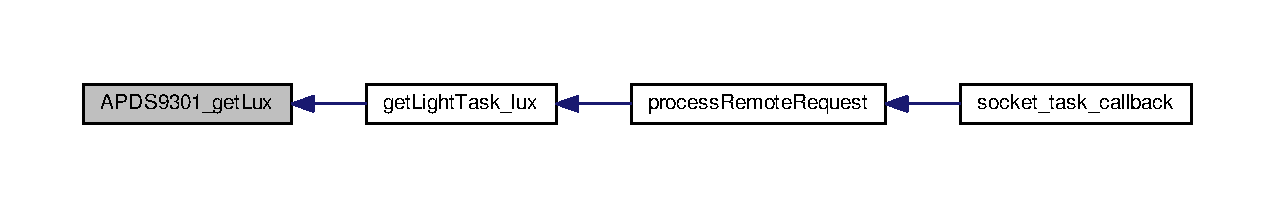
\includegraphics[width=350pt]{apds9301__sensor_8h_a55e164e7dd0586de71a8dd5b25ae9ef3_icgraph}
\end{center}
\end{figure}


\index{apds9301\+\_\+sensor.\+h@{apds9301\+\_\+sensor.\+h}!A\+P\+D\+S9301\+\_\+mem\+Dump@{A\+P\+D\+S9301\+\_\+mem\+Dump}}
\index{A\+P\+D\+S9301\+\_\+mem\+Dump@{A\+P\+D\+S9301\+\_\+mem\+Dump}!apds9301\+\_\+sensor.\+h@{apds9301\+\_\+sensor.\+h}}
\subsubsection[{\texorpdfstring{A\+P\+D\+S9301\+\_\+mem\+Dump()}{APDS9301_memDump()}}]{\setlength{\rightskip}{0pt plus 5cm}uint8\+\_\+t$\ast$ A\+P\+D\+S9301\+\_\+mem\+Dump (
\begin{DoxyParamCaption}
{}
\end{DoxyParamCaption}
)}\hypertarget{apds9301__sensor_8h_acae5d5b1cfb4008743589e5482d7578b}{}\label{apds9301__sensor_8h_acae5d5b1cfb4008743589e5482d7578b}


Gives a memdump of 15 len. {\bfseries I\+MP} must free the address using return pointer. 

\begin{DoxyReturn}{Returns}
uint8\+\_\+t$\ast$ 
\end{DoxyReturn}

\begin{DoxyCode}
235 \{
236     uint8\_t *memdump = (uint8\_t*)malloc(15*\textcolor{keyword}{sizeof}(uint8\_t));
237     memset(memdump, 0 , 15);
238 
239     \textcolor{keywordflow}{for}(uint8\_t i = 0 ; i < 0x10; i++)
240     \{
241         \textcolor{keywordflow}{if}(i == 0x7 ||  i == 0x9 || i == 0xB)
242             \textcolor{keywordflow}{continue};
243         
244         \textcolor{keywordtype}{int} ret = \hyperlink{my__i2c_8c_a8024ad1f3558034ee998758f45d456d9}{I2Cmaster\_read\_byte}(APDS9301\_SLAVE\_ADDR, i | APDS9301\_CMD\_REG, memdump
      +i);
245         \textcolor{keywordflow}{if}(ret != 0 ) \textcolor{keywordflow}{continue};
246     \}
247 
248     \textcolor{keywordflow}{return} memdump;
249 \}
\end{DoxyCode}
\index{apds9301\+\_\+sensor.\+h@{apds9301\+\_\+sensor.\+h}!A\+P\+D\+S9301\+\_\+mode\+\_\+high\+Gain@{A\+P\+D\+S9301\+\_\+mode\+\_\+high\+Gain}}
\index{A\+P\+D\+S9301\+\_\+mode\+\_\+high\+Gain@{A\+P\+D\+S9301\+\_\+mode\+\_\+high\+Gain}!apds9301\+\_\+sensor.\+h@{apds9301\+\_\+sensor.\+h}}
\subsubsection[{\texorpdfstring{A\+P\+D\+S9301\+\_\+mode\+\_\+high\+Gain()}{APDS9301_mode_highGain()}}]{\setlength{\rightskip}{0pt plus 5cm}int A\+P\+D\+S9301\+\_\+mode\+\_\+high\+Gain (
\begin{DoxyParamCaption}
{}
\end{DoxyParamCaption}
)}\hypertarget{apds9301__sensor_8h_a5e527c870fed599e87d712a151e47172}{}\label{apds9301__sensor_8h_a5e527c870fed599e87d712a151e47172}
\begin{DoxyReturn}{Returns}
int 
\end{DoxyReturn}

\begin{DoxyCode}
61 \{
62     uint8\_t data;
63     \textcolor{keywordtype}{int} ret = \hyperlink{my__i2c_8c_a8024ad1f3558034ee998758f45d456d9}{I2Cmaster\_read\_byte}(APDS9301\_SLAVE\_ADDR, APDS9301\_TIMING\_REG, &data);
64     \textcolor{keywordflow}{if}(ret != 0)
65         \textcolor{keywordflow}{return} ret;
66 
67     data |= (uint8\_t)APDS9301\_TIMING\_GAIN;
68 
69     ret = \hyperlink{my__i2c_8c_a202be1d68320e3ba93c759821ba2f695}{I2Cmaster\_write\_byte}(APDS9301\_SLAVE\_ADDR, APDS9301\_TIMING\_REG, data);
70 
71     \textcolor{keywordflow}{return} ret;
72 \}
\end{DoxyCode}
\index{apds9301\+\_\+sensor.\+h@{apds9301\+\_\+sensor.\+h}!A\+P\+D\+S9301\+\_\+mode\+\_\+integration\+Time@{A\+P\+D\+S9301\+\_\+mode\+\_\+integration\+Time}}
\index{A\+P\+D\+S9301\+\_\+mode\+\_\+integration\+Time@{A\+P\+D\+S9301\+\_\+mode\+\_\+integration\+Time}!apds9301\+\_\+sensor.\+h@{apds9301\+\_\+sensor.\+h}}
\subsubsection[{\texorpdfstring{A\+P\+D\+S9301\+\_\+mode\+\_\+integration\+Time(uint8\+\_\+t x)}{APDS9301_mode_integrationTime(uint8_t x)}}]{\setlength{\rightskip}{0pt plus 5cm}int A\+P\+D\+S9301\+\_\+mode\+\_\+integration\+Time (
\begin{DoxyParamCaption}
\item[{uint8\+\_\+t}]{x}
\end{DoxyParamCaption}
)}\hypertarget{apds9301__sensor_8h_ac14a5a102513243824d12e6028abbeb8}{}\label{apds9301__sensor_8h_ac14a5a102513243824d12e6028abbeb8}

\begin{DoxyParams}{Parameters}
{\em x} & \\
\hline
\end{DoxyParams}
\begin{DoxyReturn}{Returns}
int 
\end{DoxyReturn}

\begin{DoxyCode}
126 \{
127     uint8\_t data;
128     \textcolor{keywordtype}{int} ret = \hyperlink{my__i2c_8c_a8024ad1f3558034ee998758f45d456d9}{I2Cmaster\_read\_byte}(APDS9301\_SLAVE\_ADDR, APDS9301\_TIMING\_REG, &data);
129     \textcolor{keywordflow}{if}(ret != 0)
130         \textcolor{keywordflow}{return} ret;
131     
132     data &= ~(uint8\_t)APDS9301\_TIMING\_INTEG(3);
133     data |= (uint8\_t)APDS9301\_TIMING\_INTEG(x);
134 
135     ret = \hyperlink{my__i2c_8c_a202be1d68320e3ba93c759821ba2f695}{I2Cmaster\_write\_byte}(APDS9301\_SLAVE\_ADDR, APDS9301\_TIMING\_REG, data);
136 
137     \textcolor{keywordflow}{return} ret;
138 \}
\end{DoxyCode}
\index{apds9301\+\_\+sensor.\+h@{apds9301\+\_\+sensor.\+h}!A\+P\+D\+S9301\+\_\+mode\+\_\+interrupt@{A\+P\+D\+S9301\+\_\+mode\+\_\+interrupt}}
\index{A\+P\+D\+S9301\+\_\+mode\+\_\+interrupt@{A\+P\+D\+S9301\+\_\+mode\+\_\+interrupt}!apds9301\+\_\+sensor.\+h@{apds9301\+\_\+sensor.\+h}}
\subsubsection[{\texorpdfstring{A\+P\+D\+S9301\+\_\+mode\+\_\+interrupt(uint8\+\_\+t enable)}{APDS9301_mode_interrupt(uint8_t enable)}}]{\setlength{\rightskip}{0pt plus 5cm}int A\+P\+D\+S9301\+\_\+mode\+\_\+interrupt (
\begin{DoxyParamCaption}
\item[{uint8\+\_\+t}]{enable}
\end{DoxyParamCaption}
)}\hypertarget{apds9301__sensor_8h_a69d91df573c8c448a30715ae605262d7}{}\label{apds9301__sensor_8h_a69d91df573c8c448a30715ae605262d7}

\begin{DoxyParams}{Parameters}
{\em enable} & \\
\hline
\end{DoxyParams}
\begin{DoxyReturn}{Returns}
int 
\end{DoxyReturn}

\begin{DoxyCode}
89 \{
90     uint8\_t data;
91     \textcolor{keywordtype}{int} ret = \hyperlink{my__i2c_8c_a8024ad1f3558034ee998758f45d456d9}{I2Cmaster\_read\_byte}(APDS9301\_SLAVE\_ADDR, APDS9301\_INT\_CTRL\_REG, &data);
92     \textcolor{keywordflow}{if}(ret != 0)
93         \textcolor{keywordflow}{return} ret;
94 
95     \textcolor{keywordflow}{if}(enable)
96         data |= (uint8\_t)APDS9301\_INTCTRL\_IEN;
97     \textcolor{keywordflow}{else}
98         data &= ~(uint8\_t)APDS9301\_INTCTRL\_IEN;
99 
100     ret = \hyperlink{my__i2c_8c_a202be1d68320e3ba93c759821ba2f695}{I2Cmaster\_write\_byte}(APDS9301\_SLAVE\_ADDR, APDS9301\_INT\_CTRL\_REG, data);
101 
102     \textcolor{keywordflow}{return} ret;
103 \}
\end{DoxyCode}
\index{apds9301\+\_\+sensor.\+h@{apds9301\+\_\+sensor.\+h}!A\+P\+D\+S9301\+\_\+mode\+\_\+low\+Gain\+\_\+default@{A\+P\+D\+S9301\+\_\+mode\+\_\+low\+Gain\+\_\+default}}
\index{A\+P\+D\+S9301\+\_\+mode\+\_\+low\+Gain\+\_\+default@{A\+P\+D\+S9301\+\_\+mode\+\_\+low\+Gain\+\_\+default}!apds9301\+\_\+sensor.\+h@{apds9301\+\_\+sensor.\+h}}
\subsubsection[{\texorpdfstring{A\+P\+D\+S9301\+\_\+mode\+\_\+low\+Gain\+\_\+default()}{APDS9301_mode_lowGain_default()}}]{\setlength{\rightskip}{0pt plus 5cm}int A\+P\+D\+S9301\+\_\+mode\+\_\+low\+Gain\+\_\+default (
\begin{DoxyParamCaption}
{}
\end{DoxyParamCaption}
)}\hypertarget{apds9301__sensor_8h_aa8c71ee19fe0ef5ff8880f87daa2757a}{}\label{apds9301__sensor_8h_aa8c71ee19fe0ef5ff8880f87daa2757a}
\begin{DoxyReturn}{Returns}
int 
\end{DoxyReturn}

\begin{DoxyCode}
74 \{
75     uint8\_t data;
76     \textcolor{keywordtype}{int} ret = \hyperlink{my__i2c_8c_a8024ad1f3558034ee998758f45d456d9}{I2Cmaster\_read\_byte}(APDS9301\_SLAVE\_ADDR, APDS9301\_TIMING\_REG, &data);
77     \textcolor{keywordflow}{if}(ret != 0)
78         \textcolor{keywordflow}{return} ret;
79 
80     data &= ~(uint8\_t)APDS9301\_TIMING\_GAIN;
81 
82     ret = \hyperlink{my__i2c_8c_a202be1d68320e3ba93c759821ba2f695}{I2Cmaster\_write\_byte}(APDS9301\_SLAVE\_ADDR, APDS9301\_TIMING\_REG, data);
83 
84     \textcolor{keywordflow}{return} ret;
85 
86 \}
\end{DoxyCode}


Here is the caller graph for this function\+:\nopagebreak
\begin{figure}[H]
\begin{center}
\leavevmode
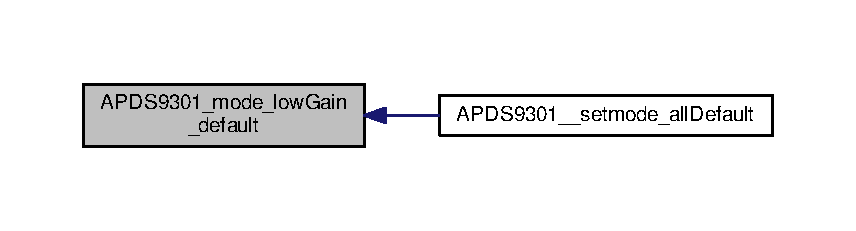
\includegraphics[width=350pt]{apds9301__sensor_8h_aa8c71ee19fe0ef5ff8880f87daa2757a_icgraph}
\end{center}
\end{figure}


\index{apds9301\+\_\+sensor.\+h@{apds9301\+\_\+sensor.\+h}!A\+P\+D\+S9301\+\_\+mode\+\_\+manualcontrol@{A\+P\+D\+S9301\+\_\+mode\+\_\+manualcontrol}}
\index{A\+P\+D\+S9301\+\_\+mode\+\_\+manualcontrol@{A\+P\+D\+S9301\+\_\+mode\+\_\+manualcontrol}!apds9301\+\_\+sensor.\+h@{apds9301\+\_\+sensor.\+h}}
\subsubsection[{\texorpdfstring{A\+P\+D\+S9301\+\_\+mode\+\_\+manualcontrol(uint8\+\_\+t on)}{APDS9301_mode_manualcontrol(uint8_t on)}}]{\setlength{\rightskip}{0pt plus 5cm}int A\+P\+D\+S9301\+\_\+mode\+\_\+manualcontrol (
\begin{DoxyParamCaption}
\item[{uint8\+\_\+t}]{on}
\end{DoxyParamCaption}
)}\hypertarget{apds9301__sensor_8h_ad22326035668d08e6d7cade8cde126e4}{}\label{apds9301__sensor_8h_ad22326035668d08e6d7cade8cde126e4}

\begin{DoxyParams}{Parameters}
{\em on} & \\
\hline
\end{DoxyParams}
\begin{DoxyReturn}{Returns}
int 
\end{DoxyReturn}

\begin{DoxyCode}
111 \{
112     uint8\_t data;
113     \textcolor{keywordtype}{int} ret = \hyperlink{my__i2c_8c_a8024ad1f3558034ee998758f45d456d9}{I2Cmaster\_read\_byte}(APDS9301\_SLAVE\_ADDR, APDS9301\_TIMING\_REG, &data);
114     \textcolor{keywordflow}{if}(ret != 0)
115         \textcolor{keywordflow}{return} ret;
116 
117     data &= ~(uint8\_t)APDS9301\_TIMING\_MANUAL(1);
118     data |= (uint8\_t)APDS9301\_TIMING\_MANUAL(on);
119 
120     ret = \hyperlink{my__i2c_8c_a202be1d68320e3ba93c759821ba2f695}{I2Cmaster\_write\_byte}(APDS9301\_SLAVE\_ADDR, APDS9301\_TIMING\_REG, data);
121 
122     \textcolor{keywordflow}{return} ret;
123 \}
\end{DoxyCode}
\index{apds9301\+\_\+sensor.\+h@{apds9301\+\_\+sensor.\+h}!A\+P\+D\+S9301\+\_\+powerdown@{A\+P\+D\+S9301\+\_\+powerdown}}
\index{A\+P\+D\+S9301\+\_\+powerdown@{A\+P\+D\+S9301\+\_\+powerdown}!apds9301\+\_\+sensor.\+h@{apds9301\+\_\+sensor.\+h}}
\subsubsection[{\texorpdfstring{A\+P\+D\+S9301\+\_\+powerdown()}{APDS9301_powerdown()}}]{\setlength{\rightskip}{0pt plus 5cm}int A\+P\+D\+S9301\+\_\+powerdown (
\begin{DoxyParamCaption}
{}
\end{DoxyParamCaption}
)}\hypertarget{apds9301__sensor_8h_a2ddb9f93c9fac9cb3fbe152bda7bc43b}{}\label{apds9301__sensor_8h_a2ddb9f93c9fac9cb3fbe152bda7bc43b}
\begin{DoxyReturn}{Returns}
int 
\end{DoxyReturn}

\begin{DoxyCode}
147 \{
148     \textcolor{keywordtype}{int} ret = \hyperlink{my__i2c_8c_a202be1d68320e3ba93c759821ba2f695}{I2Cmaster\_write\_byte}(APDS9301\_SLAVE\_ADDR, APDS9301\_CTRL\_REG, 
      APDS9301\_CTRL\_POWEROFF);
149     \textcolor{keywordflow}{return} ret;
150 \}
\end{DoxyCode}


Here is the caller graph for this function\+:\nopagebreak
\begin{figure}[H]
\begin{center}
\leavevmode
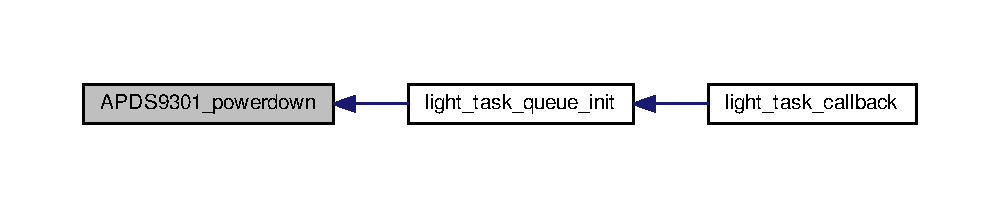
\includegraphics[width=350pt]{apds9301__sensor_8h_a2ddb9f93c9fac9cb3fbe152bda7bc43b_icgraph}
\end{center}
\end{figure}


\index{apds9301\+\_\+sensor.\+h@{apds9301\+\_\+sensor.\+h}!A\+P\+D\+S9301\+\_\+poweron@{A\+P\+D\+S9301\+\_\+poweron}}
\index{A\+P\+D\+S9301\+\_\+poweron@{A\+P\+D\+S9301\+\_\+poweron}!apds9301\+\_\+sensor.\+h@{apds9301\+\_\+sensor.\+h}}
\subsubsection[{\texorpdfstring{A\+P\+D\+S9301\+\_\+poweron()}{APDS9301_poweron()}}]{\setlength{\rightskip}{0pt plus 5cm}int A\+P\+D\+S9301\+\_\+poweron (
\begin{DoxyParamCaption}
{}
\end{DoxyParamCaption}
)}\hypertarget{apds9301__sensor_8h_a5f0928561f20743cccb1a4f6336ddff4}{}\label{apds9301__sensor_8h_a5f0928561f20743cccb1a4f6336ddff4}
\begin{DoxyReturn}{Returns}
int 
\end{DoxyReturn}

\begin{DoxyCode}
142 \{
143     \textcolor{keywordtype}{int} ret = \hyperlink{my__i2c_8c_a202be1d68320e3ba93c759821ba2f695}{I2Cmaster\_write\_byte}(APDS9301\_SLAVE\_ADDR, APDS9301\_CTRL\_REG, 
      APDS9301\_CTRL\_POWERON);
144     \textcolor{keywordflow}{return} ret;
145 \}
\end{DoxyCode}


Here is the caller graph for this function\+:\nopagebreak
\begin{figure}[H]
\begin{center}
\leavevmode
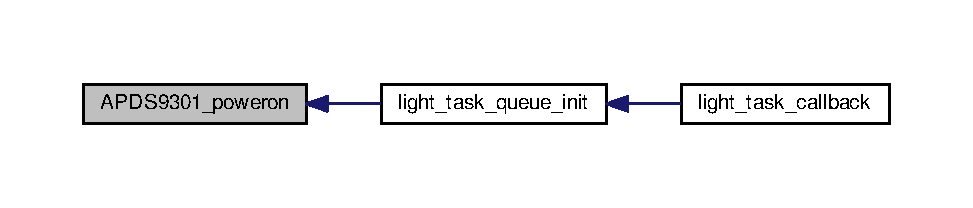
\includegraphics[width=350pt]{apds9301__sensor_8h_a5f0928561f20743cccb1a4f6336ddff4_icgraph}
\end{center}
\end{figure}


\index{apds9301\+\_\+sensor.\+h@{apds9301\+\_\+sensor.\+h}!A\+P\+D\+S9301\+\_\+read\+\_\+\+Th\+High@{A\+P\+D\+S9301\+\_\+read\+\_\+\+Th\+High}}
\index{A\+P\+D\+S9301\+\_\+read\+\_\+\+Th\+High@{A\+P\+D\+S9301\+\_\+read\+\_\+\+Th\+High}!apds9301\+\_\+sensor.\+h@{apds9301\+\_\+sensor.\+h}}
\subsubsection[{\texorpdfstring{A\+P\+D\+S9301\+\_\+read\+\_\+\+Th\+High(uint16\+\_\+t $\ast$thhigh)}{APDS9301_read_ThHigh(uint16_t *thhigh)}}]{\setlength{\rightskip}{0pt plus 5cm}int A\+P\+D\+S9301\+\_\+read\+\_\+\+Th\+High (
\begin{DoxyParamCaption}
\item[{uint16\+\_\+t $\ast$}]{thhigh}
\end{DoxyParamCaption}
)}\hypertarget{apds9301__sensor_8h_ab7d8d5ac5b780bcdb0a399f286b7f224}{}\label{apds9301__sensor_8h_ab7d8d5ac5b780bcdb0a399f286b7f224}

\begin{DoxyParams}{Parameters}
{\em thhigh} & \\
\hline
\end{DoxyParams}
\begin{DoxyReturn}{Returns}
int 
\end{DoxyReturn}

\begin{DoxyCode}
49 \{
50     \textcolor{keywordtype}{int} ret = \hyperlink{my__i2c_8c_ab25650a9cf74e65561b1fced3555f36c}{I2Cmaster\_read\_bytes}(APDS9301\_SLAVE\_ADDR, APDS9301\_INT\_TH\_HL\_REG, (
      uint8\_t*)thhigh, \textcolor{keyword}{sizeof}(thhigh));
51     \textcolor{keywordflow}{return} ret;
52 \}
\end{DoxyCode}
\index{apds9301\+\_\+sensor.\+h@{apds9301\+\_\+sensor.\+h}!A\+P\+D\+S9301\+\_\+read\+\_\+\+Th\+Low@{A\+P\+D\+S9301\+\_\+read\+\_\+\+Th\+Low}}
\index{A\+P\+D\+S9301\+\_\+read\+\_\+\+Th\+Low@{A\+P\+D\+S9301\+\_\+read\+\_\+\+Th\+Low}!apds9301\+\_\+sensor.\+h@{apds9301\+\_\+sensor.\+h}}
\subsubsection[{\texorpdfstring{A\+P\+D\+S9301\+\_\+read\+\_\+\+Th\+Low(uint16\+\_\+t $\ast$thlow)}{APDS9301_read_ThLow(uint16_t *thlow)}}]{\setlength{\rightskip}{0pt plus 5cm}int A\+P\+D\+S9301\+\_\+read\+\_\+\+Th\+Low (
\begin{DoxyParamCaption}
\item[{uint16\+\_\+t $\ast$}]{thlow}
\end{DoxyParamCaption}
)}\hypertarget{apds9301__sensor_8h_ad0dcd5037cad9e4ed654da7d9d548010}{}\label{apds9301__sensor_8h_ad0dcd5037cad9e4ed654da7d9d548010}

\begin{DoxyParams}{Parameters}
{\em thlow} & \\
\hline
\end{DoxyParams}
\begin{DoxyReturn}{Returns}
int 
\end{DoxyReturn}

\begin{DoxyCode}
43 \{
44     \textcolor{keywordtype}{int} ret = \hyperlink{my__i2c_8c_ab25650a9cf74e65561b1fced3555f36c}{I2Cmaster\_read\_bytes}(APDS9301\_SLAVE\_ADDR, APDS9301\_INT\_TH\_LL\_REG, (
      uint8\_t*)thlow, \textcolor{keyword}{sizeof}(thlow));
45     \textcolor{keywordflow}{return} ret;
46 \}
\end{DoxyCode}
\index{apds9301\+\_\+sensor.\+h@{apds9301\+\_\+sensor.\+h}!A\+P\+D\+S9301\+\_\+read\+Ch0@{A\+P\+D\+S9301\+\_\+read\+Ch0}}
\index{A\+P\+D\+S9301\+\_\+read\+Ch0@{A\+P\+D\+S9301\+\_\+read\+Ch0}!apds9301\+\_\+sensor.\+h@{apds9301\+\_\+sensor.\+h}}
\subsubsection[{\texorpdfstring{A\+P\+D\+S9301\+\_\+read\+Ch0(uint16\+\_\+t $\ast$ch0\+\_\+data)}{APDS9301_readCh0(uint16_t *ch0_data)}}]{\setlength{\rightskip}{0pt plus 5cm}int A\+P\+D\+S9301\+\_\+read\+Ch0 (
\begin{DoxyParamCaption}
\item[{uint16\+\_\+t $\ast$}]{ch0\+\_\+data}
\end{DoxyParamCaption}
)}\hypertarget{apds9301__sensor_8h_ae41babc910792ba1bbb19e837fd45d4c}{}\label{apds9301__sensor_8h_ae41babc910792ba1bbb19e837fd45d4c}

\begin{DoxyParams}{Parameters}
{\em ch0\+\_\+data} & \\
\hline
\end{DoxyParams}
\begin{DoxyReturn}{Returns}
int 
\end{DoxyReturn}

\begin{DoxyCode}
158 \{
159     \textcolor{keywordtype}{int} ret;
160     uint8\_t ch0\_data\_L, ch0\_data\_H;
161     ret = \hyperlink{my__i2c_8c_a8024ad1f3558034ee998758f45d456d9}{I2Cmaster\_read\_byte}(APDS9301\_SLAVE\_ADDR, APDS9301\_CH0\_DATALOW, &ch0\_data\_L);
162     \textcolor{keywordflow}{if}(ret)
163         \textcolor{keywordflow}{return} ret;
164 
165     ret = \hyperlink{my__i2c_8c_a8024ad1f3558034ee998758f45d456d9}{I2Cmaster\_read\_byte}(APDS9301\_SLAVE\_ADDR, APDS9301\_CH0\_DATAHIGH, &ch0\_data\_H);
166 
167     \textcolor{keywordflow}{if}(!ret)
168         *ch0\_data = (ch0\_data\_H << 8) | ch0\_data\_L ;
169     
170     \textcolor{keywordflow}{return} ret;
171 \}
\end{DoxyCode}


Here is the caller graph for this function\+:\nopagebreak
\begin{figure}[H]
\begin{center}
\leavevmode
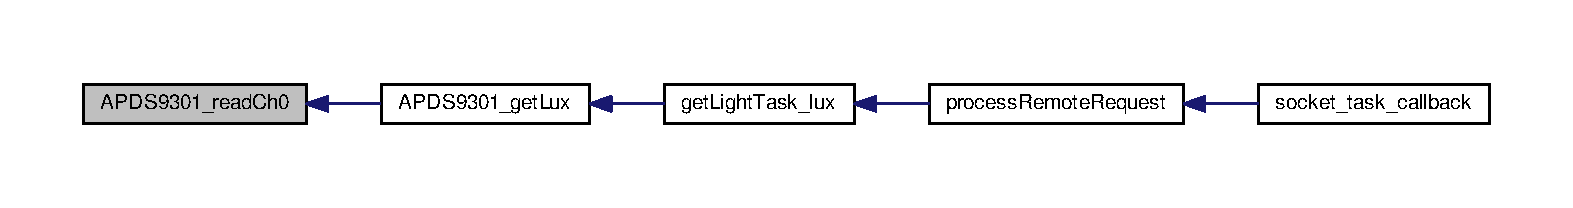
\includegraphics[width=350pt]{apds9301__sensor_8h_ae41babc910792ba1bbb19e837fd45d4c_icgraph}
\end{center}
\end{figure}


\index{apds9301\+\_\+sensor.\+h@{apds9301\+\_\+sensor.\+h}!A\+P\+D\+S9301\+\_\+read\+Ch1@{A\+P\+D\+S9301\+\_\+read\+Ch1}}
\index{A\+P\+D\+S9301\+\_\+read\+Ch1@{A\+P\+D\+S9301\+\_\+read\+Ch1}!apds9301\+\_\+sensor.\+h@{apds9301\+\_\+sensor.\+h}}
\subsubsection[{\texorpdfstring{A\+P\+D\+S9301\+\_\+read\+Ch1(uint16\+\_\+t $\ast$ch1\+\_\+data)}{APDS9301_readCh1(uint16_t *ch1_data)}}]{\setlength{\rightskip}{0pt plus 5cm}int A\+P\+D\+S9301\+\_\+read\+Ch1 (
\begin{DoxyParamCaption}
\item[{uint16\+\_\+t $\ast$}]{ch1\+\_\+data}
\end{DoxyParamCaption}
)}\hypertarget{apds9301__sensor_8h_a34c034b815ceb2e30b0161d7461f0a8e}{}\label{apds9301__sensor_8h_a34c034b815ceb2e30b0161d7461f0a8e}

\begin{DoxyParams}{Parameters}
{\em ch1\+\_\+data} & \\
\hline
\end{DoxyParams}
\begin{DoxyReturn}{Returns}
int 
\end{DoxyReturn}

\begin{DoxyCode}
174 \{
175     \textcolor{keywordtype}{int} ret;
176     uint8\_t ch1\_data\_L, ch1\_data\_H;
177     ret = \hyperlink{my__i2c_8c_a8024ad1f3558034ee998758f45d456d9}{I2Cmaster\_read\_byte}(APDS9301\_SLAVE\_ADDR, APDS9301\_CH1\_DATALOW, &ch1\_data\_L);
178     \textcolor{keywordflow}{if}(ret)
179         \textcolor{keywordflow}{return} ret;
180 
181     ret = \hyperlink{my__i2c_8c_a8024ad1f3558034ee998758f45d456d9}{I2Cmaster\_read\_byte}(APDS9301\_SLAVE\_ADDR, APDS9301\_CH1\_DATAHIGH, &ch1\_data\_H);
182     
183     \textcolor{keywordflow}{if}(!ret)
184         *ch1\_data = (ch1\_data\_H << 8) | ch1\_data\_L;
185     
186     \textcolor{keywordflow}{return} ret;
187 
188 \}
\end{DoxyCode}


Here is the caller graph for this function\+:\nopagebreak
\begin{figure}[H]
\begin{center}
\leavevmode
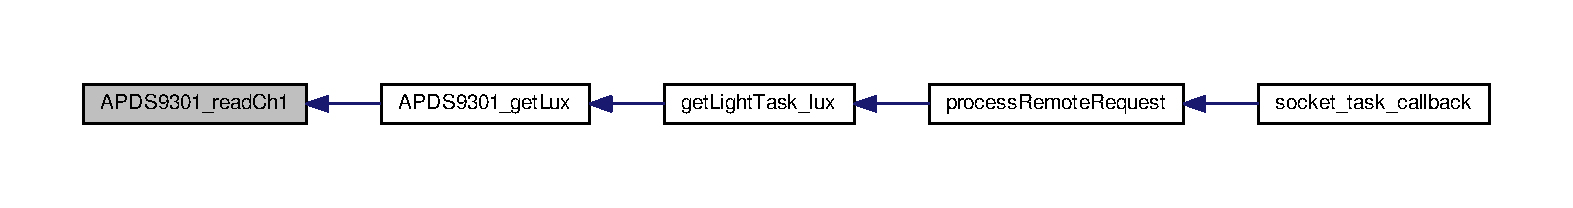
\includegraphics[width=350pt]{apds9301__sensor_8h_a34c034b815ceb2e30b0161d7461f0a8e_icgraph}
\end{center}
\end{figure}


\index{apds9301\+\_\+sensor.\+h@{apds9301\+\_\+sensor.\+h}!A\+P\+D\+S9301\+\_\+read\+Control\+Reg@{A\+P\+D\+S9301\+\_\+read\+Control\+Reg}}
\index{A\+P\+D\+S9301\+\_\+read\+Control\+Reg@{A\+P\+D\+S9301\+\_\+read\+Control\+Reg}!apds9301\+\_\+sensor.\+h@{apds9301\+\_\+sensor.\+h}}
\subsubsection[{\texorpdfstring{A\+P\+D\+S9301\+\_\+read\+Control\+Reg(uint8\+\_\+t $\ast$ctrl\+\_\+reg)}{APDS9301_readControlReg(uint8_t *ctrl_reg)}}]{\setlength{\rightskip}{0pt plus 5cm}int A\+P\+D\+S9301\+\_\+read\+Control\+Reg (
\begin{DoxyParamCaption}
\item[{uint8\+\_\+t $\ast$}]{ctrl\+\_\+reg}
\end{DoxyParamCaption}
)}\hypertarget{apds9301__sensor_8h_a2aa3244d3848324ba9f4afc7b1990ce1}{}\label{apds9301__sensor_8h_a2aa3244d3848324ba9f4afc7b1990ce1}

\begin{DoxyParams}{Parameters}
{\em ctrl\+\_\+reg} & \\
\hline
\end{DoxyParams}
\begin{DoxyReturn}{Returns}
int 
\end{DoxyReturn}

\begin{DoxyCode}
55 \{
56     \textcolor{keywordtype}{int} ret = \hyperlink{my__i2c_8c_a8024ad1f3558034ee998758f45d456d9}{I2Cmaster\_read\_byte}(APDS9301\_SLAVE\_ADDR, APDS9301\_CTRL\_REG, ctrl\_reg);
57     \textcolor{keywordflow}{return} ret;
58 \}
\end{DoxyCode}
\index{apds9301\+\_\+sensor.\+h@{apds9301\+\_\+sensor.\+h}!A\+P\+D\+S9301\+\_\+read\+ID@{A\+P\+D\+S9301\+\_\+read\+ID}}
\index{A\+P\+D\+S9301\+\_\+read\+ID@{A\+P\+D\+S9301\+\_\+read\+ID}!apds9301\+\_\+sensor.\+h@{apds9301\+\_\+sensor.\+h}}
\subsubsection[{\texorpdfstring{A\+P\+D\+S9301\+\_\+read\+I\+D(uint8\+\_\+t $\ast$id)}{APDS9301_readID(uint8_t *id)}}]{\setlength{\rightskip}{0pt plus 5cm}int A\+P\+D\+S9301\+\_\+read\+ID (
\begin{DoxyParamCaption}
\item[{uint8\+\_\+t $\ast$}]{id}
\end{DoxyParamCaption}
)}\hypertarget{apds9301__sensor_8h_a82dac2bc9fc0e11fc4589f3492bec13e}{}\label{apds9301__sensor_8h_a82dac2bc9fc0e11fc4589f3492bec13e}

\begin{DoxyParams}{Parameters}
{\em id} & \\
\hline
\end{DoxyParams}
\begin{DoxyReturn}{Returns}
int 
\end{DoxyReturn}

\begin{DoxyCode}
152 \{
153     \textcolor{keywordtype}{int} ret = \hyperlink{my__i2c_8c_a8024ad1f3558034ee998758f45d456d9}{I2Cmaster\_read\_byte}(APDS9301\_SLAVE\_ADDR, APDS9301\_ID\_REG, \textcolor{keywordtype}{id});
154     \textcolor{keywordflow}{return} ret;
155 \}
\end{DoxyCode}


Here is the caller graph for this function\+:\nopagebreak
\begin{figure}[H]
\begin{center}
\leavevmode
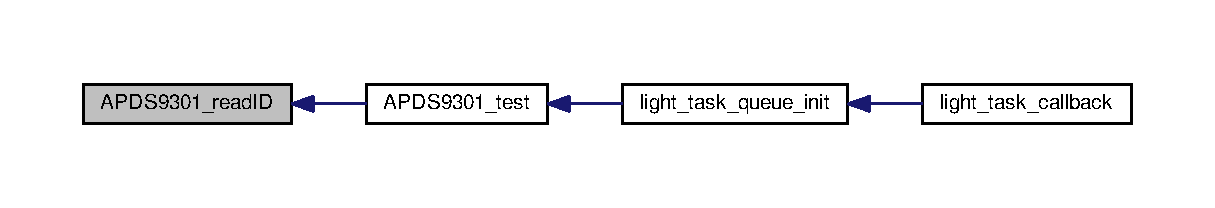
\includegraphics[width=350pt]{apds9301__sensor_8h_a82dac2bc9fc0e11fc4589f3492bec13e_icgraph}
\end{center}
\end{figure}


\index{apds9301\+\_\+sensor.\+h@{apds9301\+\_\+sensor.\+h}!A\+P\+D\+S9301\+\_\+test@{A\+P\+D\+S9301\+\_\+test}}
\index{A\+P\+D\+S9301\+\_\+test@{A\+P\+D\+S9301\+\_\+test}!apds9301\+\_\+sensor.\+h@{apds9301\+\_\+sensor.\+h}}
\subsubsection[{\texorpdfstring{A\+P\+D\+S9301\+\_\+test()}{APDS9301_test()}}]{\setlength{\rightskip}{0pt plus 5cm}int A\+P\+D\+S9301\+\_\+test (
\begin{DoxyParamCaption}
{}
\end{DoxyParamCaption}
)}\hypertarget{apds9301__sensor_8h_a29ea2301a68de775fc0281dd1b4b03aa}{}\label{apds9301__sensor_8h_a29ea2301a68de775fc0281dd1b4b03aa}
\begin{DoxyReturn}{Returns}
int 
\end{DoxyReturn}

\begin{DoxyCode}
18 \{
19     uint8\_t data;
20     \textcolor{keywordtype}{int} ret = \hyperlink{apds9301__sensor_8c_a82dac2bc9fc0e11fc4589f3492bec13e}{APDS9301\_readID}(&data);
21     \textcolor{keywordflow}{if}(ret == 0) 
22     \{
23         (APDS9301\_SENSOR\_ID == (data & 0xF0)) ? 0 : (ret = -1);
24     \}
25 
26     \textcolor{keywordflow}{return} ret; 
27     
28 \}
\end{DoxyCode}


Here is the caller graph for this function\+:\nopagebreak
\begin{figure}[H]
\begin{center}
\leavevmode
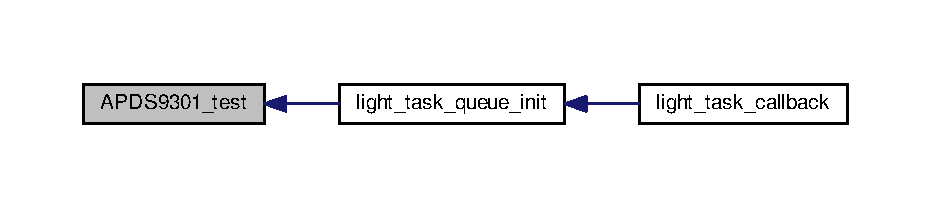
\includegraphics[width=350pt]{apds9301__sensor_8h_a29ea2301a68de775fc0281dd1b4b03aa_icgraph}
\end{center}
\end{figure}


\index{apds9301\+\_\+sensor.\+h@{apds9301\+\_\+sensor.\+h}!A\+P\+D\+S9301\+\_\+write\+\_\+\+Th\+High@{A\+P\+D\+S9301\+\_\+write\+\_\+\+Th\+High}}
\index{A\+P\+D\+S9301\+\_\+write\+\_\+\+Th\+High@{A\+P\+D\+S9301\+\_\+write\+\_\+\+Th\+High}!apds9301\+\_\+sensor.\+h@{apds9301\+\_\+sensor.\+h}}
\subsubsection[{\texorpdfstring{A\+P\+D\+S9301\+\_\+write\+\_\+\+Th\+High(uint16\+\_\+t thhigh)}{APDS9301_write_ThHigh(uint16_t thhigh)}}]{\setlength{\rightskip}{0pt plus 5cm}int A\+P\+D\+S9301\+\_\+write\+\_\+\+Th\+High (
\begin{DoxyParamCaption}
\item[{uint16\+\_\+t}]{thhigh}
\end{DoxyParamCaption}
)}\hypertarget{apds9301__sensor_8h_ad75b8b8d703f549994213adeaea90c64}{}\label{apds9301__sensor_8h_ad75b8b8d703f549994213adeaea90c64}

\begin{DoxyParams}{Parameters}
{\em thhigh} & \\
\hline
\end{DoxyParams}
\begin{DoxyReturn}{Returns}
int 
\end{DoxyReturn}

\begin{DoxyCode}
37 \{
38     \textcolor{keywordtype}{int} ret = \hyperlink{my__i2c_8c_a19c6244da5ea2d4e65a25001582498c8}{I2Cmaster\_write\_word}(APDS9301\_SLAVE\_ADDR, APDS9301\_INT\_TH\_HL\_REG | 
      APDS9301\_CMD\_WORD\_EN , thhigh, 0);
39     \textcolor{keywordflow}{return} ret;
40 \}
\end{DoxyCode}
\index{apds9301\+\_\+sensor.\+h@{apds9301\+\_\+sensor.\+h}!A\+P\+D\+S9301\+\_\+write\+\_\+\+Th\+Low@{A\+P\+D\+S9301\+\_\+write\+\_\+\+Th\+Low}}
\index{A\+P\+D\+S9301\+\_\+write\+\_\+\+Th\+Low@{A\+P\+D\+S9301\+\_\+write\+\_\+\+Th\+Low}!apds9301\+\_\+sensor.\+h@{apds9301\+\_\+sensor.\+h}}
\subsubsection[{\texorpdfstring{A\+P\+D\+S9301\+\_\+write\+\_\+\+Th\+Low(uint16\+\_\+t thlow)}{APDS9301_write_ThLow(uint16_t thlow)}}]{\setlength{\rightskip}{0pt plus 5cm}int A\+P\+D\+S9301\+\_\+write\+\_\+\+Th\+Low (
\begin{DoxyParamCaption}
\item[{uint16\+\_\+t}]{thlow}
\end{DoxyParamCaption}
)}\hypertarget{apds9301__sensor_8h_a27508ac9add1cd27cb2c143631f3a55f}{}\label{apds9301__sensor_8h_a27508ac9add1cd27cb2c143631f3a55f}

\begin{DoxyParams}{Parameters}
{\em thlow} & \\
\hline
\end{DoxyParams}
\begin{DoxyReturn}{Returns}
int 
\end{DoxyReturn}

\begin{DoxyCode}
31 \{
32     \textcolor{keywordtype}{int} ret = \hyperlink{my__i2c_8c_a19c6244da5ea2d4e65a25001582498c8}{I2Cmaster\_write\_word}(APDS9301\_SLAVE\_ADDR, APDS9301\_INT\_TH\_LL\_REG | 
      APDS9301\_CMD\_WORD\_EN, thlow, 0);
33     \textcolor{keywordflow}{return} ret;
34 \}
\end{DoxyCode}

\hypertarget{BB__Led_8h}{}\section{/home/gunj/repos/\+E\+C\+E\+N-\/5013/\+Project1/include/\+Beagle\+Bone/\+B\+B\+\_\+\+Led.h File Reference}
\label{BB__Led_8h}\index{/home/gunj/repos/\+E\+C\+E\+N-\/5013/\+Project1/include/\+Beagle\+Bone/\+B\+B\+\_\+\+Led.\+h@{/home/gunj/repos/\+E\+C\+E\+N-\/5013/\+Project1/include/\+Beagle\+Bone/\+B\+B\+\_\+\+Led.\+h}}
This graph shows which files directly or indirectly include this file\+:
\nopagebreak
\begin{figure}[H]
\begin{center}
\leavevmode
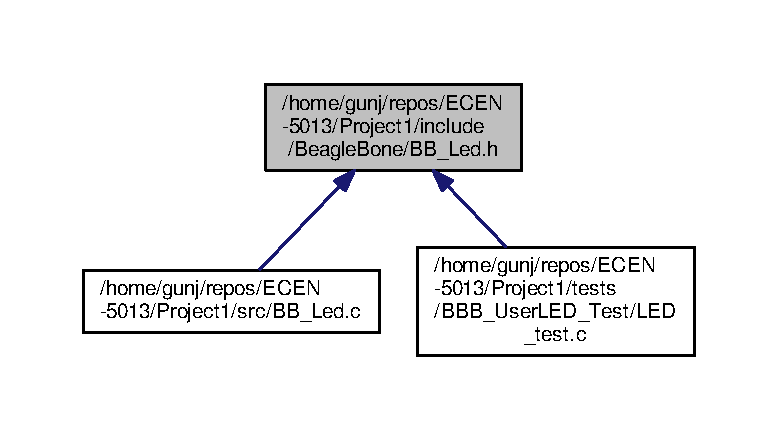
\includegraphics[width=350pt]{BB__Led_8h__dep__incl}
\end{center}
\end{figure}
\subsection*{Enumerations}
\begin{DoxyCompactItemize}
\item 
enum {\bfseries U\+S\+E\+R\+\_\+\+L\+E\+D\+\_\+T} \{ {\bfseries L\+E\+D0}, 
{\bfseries L\+E\+D1}, 
{\bfseries L\+E\+D2}, 
{\bfseries L\+E\+D3}
 \}\hypertarget{BB__Led_8h_aaf8196f69b509b42a5d7984d9b5e9f59}{}\label{BB__Led_8h_aaf8196f69b509b42a5d7984d9b5e9f59}

\end{DoxyCompactItemize}
\subsection*{Functions}
\begin{DoxyCompactItemize}
\item 
int \hyperlink{BB__Led_8h_a86628a099822bb243b1c7d57133e627b}{B\+B\+\_\+\+Led\+ON} (U\+S\+E\+R\+\_\+\+L\+E\+D\+\_\+T lednum)
\item 
int \hyperlink{BB__Led_8h_a84494234e8807c093bee8d16d7b2008b}{B\+B\+\_\+\+Led\+O\+FF} (U\+S\+E\+R\+\_\+\+L\+E\+D\+\_\+T lednum)
\item 
int \hyperlink{BB__Led_8h_a36a765a1771de0098fe83028d53827e1}{B\+B\+\_\+\+Led\+Default} ()
\end{DoxyCompactItemize}


\subsection{Detailed Description}
\begin{DoxyAuthor}{Author}
Gunj Manseta 
\end{DoxyAuthor}
\begin{DoxyDate}{Date}
2018-\/03-\/10 
\end{DoxyDate}


\subsection{Function Documentation}
\index{B\+B\+\_\+\+Led.\+h@{B\+B\+\_\+\+Led.\+h}!B\+B\+\_\+\+Led\+Default@{B\+B\+\_\+\+Led\+Default}}
\index{B\+B\+\_\+\+Led\+Default@{B\+B\+\_\+\+Led\+Default}!B\+B\+\_\+\+Led.\+h@{B\+B\+\_\+\+Led.\+h}}
\subsubsection[{\texorpdfstring{B\+B\+\_\+\+Led\+Default()}{BB_LedDefault()}}]{\setlength{\rightskip}{0pt plus 5cm}int B\+B\+\_\+\+Led\+Default (
\begin{DoxyParamCaption}
{}
\end{DoxyParamCaption}
)}\hypertarget{BB__Led_8h_a36a765a1771de0098fe83028d53827e1}{}\label{BB__Led_8h_a36a765a1771de0098fe83028d53827e1}

\begin{DoxyParams}{Parameters}
{\em lednum} & \\
\hline
\end{DoxyParams}
\begin{DoxyReturn}{Returns}
int 
\end{DoxyReturn}

\begin{DoxyCode}
70 \{
71     FILE *led\_fd = fopen(\textcolor{stringliteral}{"/sys/class/leds/beaglebone:green:usr0/trigger"}, \textcolor{stringliteral}{"r+"});
72     \textcolor{keywordflow}{if}(led\_fd)
73     \{
74         fwrite(\textcolor{stringliteral}{"heartbeat"},1,\textcolor{keyword}{sizeof}(\textcolor{stringliteral}{"heartbeat"}),led\_fd);
75         fclose(led\_fd);
76         \textcolor{keywordflow}{return} 0; 
77     \}   
78     \textcolor{keywordflow}{else}
79         \textcolor{keywordflow}{return} -1;
80 \}\end{DoxyCode}
\index{B\+B\+\_\+\+Led.\+h@{B\+B\+\_\+\+Led.\+h}!B\+B\+\_\+\+Led\+O\+FF@{B\+B\+\_\+\+Led\+O\+FF}}
\index{B\+B\+\_\+\+Led\+O\+FF@{B\+B\+\_\+\+Led\+O\+FF}!B\+B\+\_\+\+Led.\+h@{B\+B\+\_\+\+Led.\+h}}
\subsubsection[{\texorpdfstring{B\+B\+\_\+\+Led\+O\+F\+F(\+U\+S\+E\+R\+\_\+\+L\+E\+D\+\_\+\+T lednum)}{BB_LedOFF(USER_LED_T lednum)}}]{\setlength{\rightskip}{0pt plus 5cm}int B\+B\+\_\+\+Led\+O\+FF (
\begin{DoxyParamCaption}
\item[{U\+S\+E\+R\+\_\+\+L\+E\+D\+\_\+T}]{lednum}
\end{DoxyParamCaption}
)}\hypertarget{BB__Led_8h_a84494234e8807c093bee8d16d7b2008b}{}\label{BB__Led_8h_a84494234e8807c093bee8d16d7b2008b}

\begin{DoxyParams}{Parameters}
{\em lednum} & \\
\hline
\end{DoxyParams}
\begin{DoxyReturn}{Returns}
int 
\end{DoxyReturn}

\begin{DoxyCode}
49 \{
50     \textcolor{comment}{/* Forcefully using USR LED 1 */}
51     lednum = 1;
52     \textcolor{keywordflow}{if}(lednum < 4)
53     \{
54         FILE *led\_fd = fopen(LEDPATH[lednum], \textcolor{stringliteral}{"r+"});
55         \textcolor{keywordflow}{if}(led\_fd)
56         \{
57             fwrite(OFF,1,1,led\_fd);
58             fclose(led\_fd);
59             \textcolor{keywordflow}{return} 0; 
60         \}   
61         \textcolor{keywordflow}{else}
62             \textcolor{keywordflow}{return} -1;
63     \}
64     \textcolor{keywordflow}{else}
65         \textcolor{keywordflow}{return} -1;
66 
67 \}
\end{DoxyCode}
\index{B\+B\+\_\+\+Led.\+h@{B\+B\+\_\+\+Led.\+h}!B\+B\+\_\+\+Led\+ON@{B\+B\+\_\+\+Led\+ON}}
\index{B\+B\+\_\+\+Led\+ON@{B\+B\+\_\+\+Led\+ON}!B\+B\+\_\+\+Led.\+h@{B\+B\+\_\+\+Led.\+h}}
\subsubsection[{\texorpdfstring{B\+B\+\_\+\+Led\+O\+N(\+U\+S\+E\+R\+\_\+\+L\+E\+D\+\_\+\+T lednum)}{BB_LedON(USER_LED_T lednum)}}]{\setlength{\rightskip}{0pt plus 5cm}int B\+B\+\_\+\+Led\+ON (
\begin{DoxyParamCaption}
\item[{U\+S\+E\+R\+\_\+\+L\+E\+D\+\_\+T}]{lednum}
\end{DoxyParamCaption}
)}\hypertarget{BB__Led_8h_a86628a099822bb243b1c7d57133e627b}{}\label{BB__Led_8h_a86628a099822bb243b1c7d57133e627b}

\begin{DoxyParams}{Parameters}
{\em lednum} & \\
\hline
\end{DoxyParams}
\begin{DoxyReturn}{Returns}
int 
\end{DoxyReturn}

\begin{DoxyCode}
28 \{
29     \textcolor{comment}{/* Forcefully using USR LED 1 */}
30     lednum = 1;
31     \textcolor{keywordflow}{if}(lednum < 4)
32     \{
33         FILE *led\_fd = fopen(LEDPATH[lednum], \textcolor{stringliteral}{"r+"});
34         \textcolor{keywordflow}{if}(led\_fd)
35         \{
36             fwrite(ON,1,1,led\_fd);
37             fclose(led\_fd);
38             \textcolor{keywordflow}{return} 0; 
39         \}   
40         \textcolor{keywordflow}{else}
41             \textcolor{keywordflow}{return} -1;
42     \}
43     \textcolor{keywordflow}{else}
44         \textcolor{keywordflow}{return} -1;
45 
46 \}
\end{DoxyCode}

\hypertarget{my__i2c_8h}{}\section{/home/gunj/repos/\+E\+C\+E\+N-\/5013/\+Project1/include/\+Beagle\+Bone/my\+\_\+i2c.h File Reference}
\label{my__i2c_8h}\index{/home/gunj/repos/\+E\+C\+E\+N-\/5013/\+Project1/include/\+Beagle\+Bone/my\+\_\+i2c.\+h@{/home/gunj/repos/\+E\+C\+E\+N-\/5013/\+Project1/include/\+Beagle\+Bone/my\+\_\+i2c.\+h}}
{\ttfamily \#include $<$pthread.\+h$>$}\\*
{\ttfamily \#include \char`\"{}mraa/i2c.\+h\char`\"{}}\\*
Include dependency graph for my\+\_\+i2c.\+h\+:
\nopagebreak
\begin{figure}[H]
\begin{center}
\leavevmode
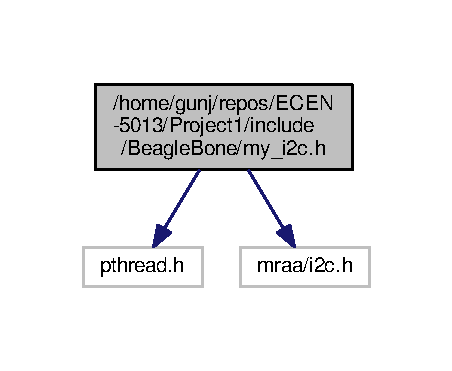
\includegraphics[width=217pt]{my__i2c_8h__incl}
\end{center}
\end{figure}
This graph shows which files directly or indirectly include this file\+:
\nopagebreak
\begin{figure}[H]
\begin{center}
\leavevmode
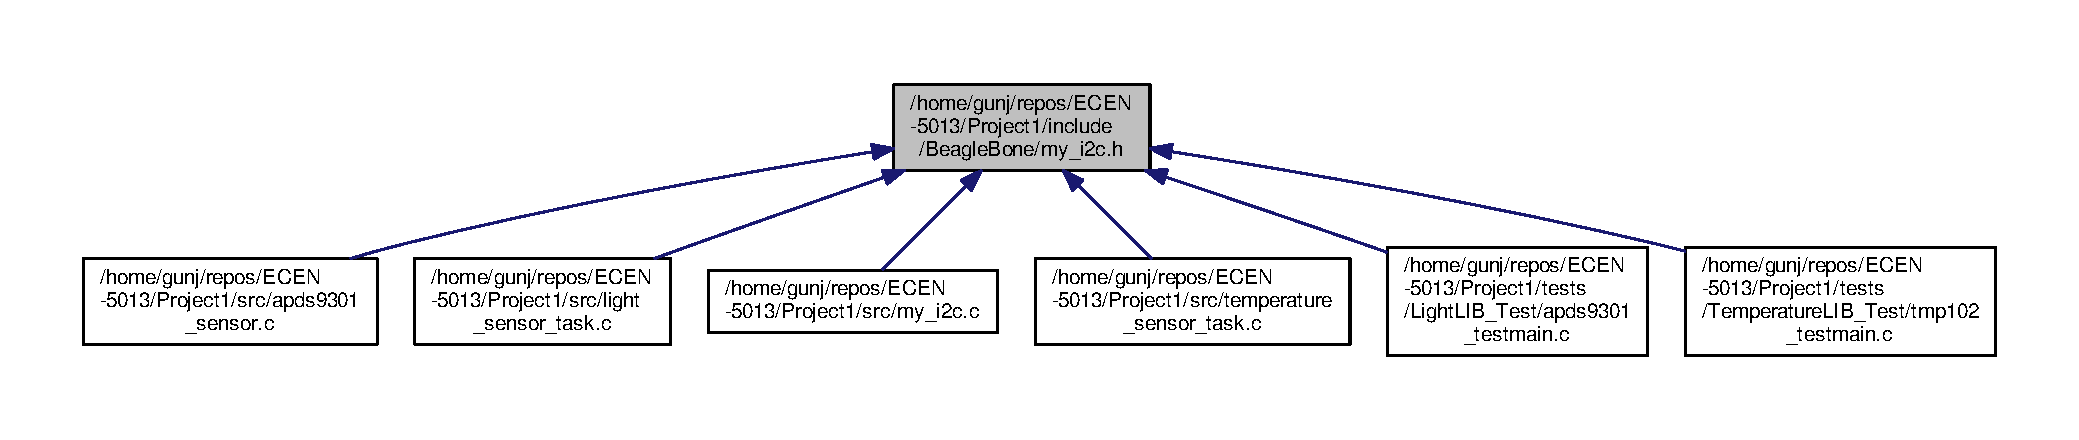
\includegraphics[width=350pt]{my__i2c_8h__dep__incl}
\end{center}
\end{figure}
\subsection*{Data Structures}
\begin{DoxyCompactItemize}
\item 
struct \hyperlink{structi2c__handle}{i2c\+\_\+handle}
\begin{DoxyCompactList}\small\item\em This is the handle for I2C mster and each master should have only one handle. \end{DoxyCompactList}\end{DoxyCompactItemize}
\subsection*{Macros}
\begin{DoxyCompactItemize}
\item 
\#define {\bfseries B\+B\+\_\+\+I2\+C\+\_\+\+B\+U\+S\+\_\+2}~(2)\hypertarget{my__i2c_8h_aa74d389e1b1373ac3449ed510de40cc7}{}\label{my__i2c_8h_aa74d389e1b1373ac3449ed510de40cc7}

\end{DoxyCompactItemize}
\subsection*{Typedefs}
\begin{DoxyCompactItemize}
\item 
typedef struct \hyperlink{structi2c__handle}{i2c\+\_\+handle} \hyperlink{my__i2c_8h_ab57e25e9caf06380c1d3587fa9866c1e}{I2\+C\+\_\+\+M\+A\+S\+T\+E\+R\+\_\+\+H\+A\+N\+D\+L\+E\+\_\+T}\hypertarget{my__i2c_8h_ab57e25e9caf06380c1d3587fa9866c1e}{}\label{my__i2c_8h_ab57e25e9caf06380c1d3587fa9866c1e}

\begin{DoxyCompactList}\small\item\em This is the handle for I2C mster and each master should have only one handle. \end{DoxyCompactList}\end{DoxyCompactItemize}
\subsection*{Functions}
\begin{DoxyCompactItemize}
\item 
\hyperlink{my__i2c_8h_ab57e25e9caf06380c1d3587fa9866c1e}{I2\+C\+\_\+\+M\+A\+S\+T\+E\+R\+\_\+\+H\+A\+N\+D\+L\+E\+\_\+T} $\ast$ \hyperlink{my__i2c_8h_a896771a0a066b06b606d35bb81809fa0}{get\+Master\+I2\+C\+\_\+handle} ()
\begin{DoxyCompactList}\small\item\em Get the Master\+I2C handle object. \end{DoxyCompactList}\item 
void \hyperlink{my__i2c_8h_a24206855ca77b181de1cfbe8e9e5051a}{print\+Error\+Code} (int error\+Code)
\begin{DoxyCompactList}\small\item\em Prints the error code string to stdout. \end{DoxyCompactList}\item 
int \hyperlink{my__i2c_8h_acea2b6a0875bf63a179959a46b3cdf7d}{I2\+Cmaster\+\_\+\+Init} (\hyperlink{my__i2c_8h_ab57e25e9caf06380c1d3587fa9866c1e}{I2\+C\+\_\+\+M\+A\+S\+T\+E\+R\+\_\+\+H\+A\+N\+D\+L\+E\+\_\+T} $\ast$handle)
\begin{DoxyCompactList}\small\item\em Inits the I2C master handle There is an internal state of the context which is maintained which gets updated with every init call Internal context goes to N\+U\+LL is error in init This context points to the new handle that is passed as the parameter. \end{DoxyCompactList}\item 
int \hyperlink{my__i2c_8h_a15136dcc397f046d0a000a781d060139}{I2\+Cmaster\+\_\+\+Destroy} (\hyperlink{my__i2c_8h_ab57e25e9caf06380c1d3587fa9866c1e}{I2\+C\+\_\+\+M\+A\+S\+T\+E\+R\+\_\+\+H\+A\+N\+D\+L\+E\+\_\+T} $\ast$handle)
\item 
int \hyperlink{my__i2c_8h_a8024ad1f3558034ee998758f45d456d9}{I2\+Cmaster\+\_\+read\+\_\+byte} (uint8\+\_\+t slave\+\_\+addr, uint8\+\_\+t reg\+\_\+addr, uint8\+\_\+t $\ast$data)
\item 
int \hyperlink{my__i2c_8h_ab25650a9cf74e65561b1fced3555f36c}{I2\+Cmaster\+\_\+read\+\_\+bytes} (uint8\+\_\+t slave\+\_\+addr, uint8\+\_\+t reg\+\_\+addr, uint8\+\_\+t $\ast$data, size\+\_\+t len)
\item 
int \hyperlink{my__i2c_8h_af92cf5a5d893ef9bbf6b4ee6de0b0ef8}{I2\+Cmaster\+\_\+write} (uint8\+\_\+t slave\+\_\+addr, uint8\+\_\+t reg\+\_\+addr)
\begin{DoxyCompactList}\small\item\em Writes a byte/pointer register to the slave. \end{DoxyCompactList}\item 
int \hyperlink{my__i2c_8h_a202be1d68320e3ba93c759821ba2f695}{I2\+Cmaster\+\_\+write\+\_\+byte} (uint8\+\_\+t slave\+\_\+addr, uint8\+\_\+t reg\+\_\+addr, uint8\+\_\+t data)
\item 
int \hyperlink{my__i2c_8h_a3a48cfc824f745c311bc081479ee6b9b}{I2\+Cmaster\+\_\+write\+\_\+bytes} (uint8\+\_\+t slave\+\_\+addr, uint8\+\_\+t reg\+\_\+addr, uint8\+\_\+t $\ast$data, size\+\_\+t len)
\item 
int \hyperlink{my__i2c_8h_a19c6244da5ea2d4e65a25001582498c8}{I2\+Cmaster\+\_\+write\+\_\+word} (uint8\+\_\+t slave\+\_\+addr, uint8\+\_\+t reg\+\_\+addr, uint16\+\_\+t data, uint8\+\_\+t lsb\+\_\+first)
\end{DoxyCompactItemize}


\subsection{Detailed Description}
\begin{DoxyAuthor}{Author}
Gunj Manseta 
\end{DoxyAuthor}
\begin{DoxyDate}{Date}
2018-\/03-\/13 
\end{DoxyDate}


\subsection{Function Documentation}
\index{my\+\_\+i2c.\+h@{my\+\_\+i2c.\+h}!get\+Master\+I2\+C\+\_\+handle@{get\+Master\+I2\+C\+\_\+handle}}
\index{get\+Master\+I2\+C\+\_\+handle@{get\+Master\+I2\+C\+\_\+handle}!my\+\_\+i2c.\+h@{my\+\_\+i2c.\+h}}
\subsubsection[{\texorpdfstring{get\+Master\+I2\+C\+\_\+handle()}{getMasterI2C_handle()}}]{\setlength{\rightskip}{0pt plus 5cm}{\bf I2\+C\+\_\+\+M\+A\+S\+T\+E\+R\+\_\+\+H\+A\+N\+D\+L\+E\+\_\+T}$\ast$ get\+Master\+I2\+C\+\_\+handle (
\begin{DoxyParamCaption}
{}
\end{DoxyParamCaption}
)}\hypertarget{my__i2c_8h_a896771a0a066b06b606d35bb81809fa0}{}\label{my__i2c_8h_a896771a0a066b06b606d35bb81809fa0}


Get the Master\+I2C handle object. 

\begin{DoxyReturn}{Returns}
I2\+C\+\_\+\+M\+A\+S\+T\+E\+R\+\_\+\+H\+A\+N\+D\+L\+E\+\_\+T $\ast$ 
\end{DoxyReturn}

\begin{DoxyCode}
108 \{
109     \textcolor{keywordflow}{return} internal\_master\_handle;
110 \}
\end{DoxyCode}
\index{my\+\_\+i2c.\+h@{my\+\_\+i2c.\+h}!I2\+Cmaster\+\_\+\+Destroy@{I2\+Cmaster\+\_\+\+Destroy}}
\index{I2\+Cmaster\+\_\+\+Destroy@{I2\+Cmaster\+\_\+\+Destroy}!my\+\_\+i2c.\+h@{my\+\_\+i2c.\+h}}
\subsubsection[{\texorpdfstring{I2\+Cmaster\+\_\+\+Destroy(\+I2\+C\+\_\+\+M\+A\+S\+T\+E\+R\+\_\+\+H\+A\+N\+D\+L\+E\+\_\+\+T $\ast$handle)}{I2Cmaster_Destroy(I2C_MASTER_HANDLE_T *handle)}}]{\setlength{\rightskip}{0pt plus 5cm}int I2\+Cmaster\+\_\+\+Destroy (
\begin{DoxyParamCaption}
\item[{{\bf I2\+C\+\_\+\+M\+A\+S\+T\+E\+R\+\_\+\+H\+A\+N\+D\+L\+E\+\_\+T} $\ast$}]{handle}
\end{DoxyParamCaption}
)}\hypertarget{my__i2c_8h_a15136dcc397f046d0a000a781d060139}{}\label{my__i2c_8h_a15136dcc397f046d0a000a781d060139}

\begin{DoxyParams}{Parameters}
{\em handle} & \\
\hline
\end{DoxyParams}
\begin{DoxyReturn}{Returns}
int 
\end{DoxyReturn}

\begin{DoxyCode}
69 \{
70     \textcolor{keywordtype}{int} ret;
71     \textcolor{keywordflow}{if}(pthread\_mutex\_lock(&init\_destroy\_lock))
72         \textcolor{keywordflow}{return} -1;
73 
74     \textcolor{comment}{/* If the input handle is not null and the input initialized handle should match the internal handle */}
          
75     \textcolor{keywordflow}{if}(NULL != handle && internal\_master\_handle == handle && NULL != internal\_master\_handle)
76     \{
77         ret = mraa\_i2c\_stop(handle->i2c\_context);
78         \textcolor{keywordflow}{if}(ret == 0)
79         \{
80             \textcolor{keyword}{static} \textcolor{keywordtype}{int} timeout = 5000;
81             \textcolor{keywordflow}{do}\{
82                 ret = pthread\_spin\_destroy(&handle->handle\_lock);
83                 timeout--;
84             \}\textcolor{keywordflow}{while}(EBUSY == ret && timeout > 0);
85 
86             \textcolor{keywordflow}{if}(ret == 0)
87             \{
88                 internal\_master\_handle = NULL;
89             \}
90         \}
91     \}
92     \textcolor{keywordflow}{else} \textcolor{keywordflow}{if}(NULL == internal\_master\_handle)
93     \{
94         ret = 0;
95     \}
96     \textcolor{keywordflow}{else} 
97     \{
98         ret = -1;
99     \}
100 
101     \textcolor{keywordflow}{if}(pthread\_mutex\_unlock(&init\_destroy\_lock))
102         \textcolor{keywordflow}{return} -1;
103 
104     \textcolor{keywordflow}{return} ret;
105 \} 
\end{DoxyCode}


Here is the caller graph for this function\+:
\nopagebreak
\begin{figure}[H]
\begin{center}
\leavevmode
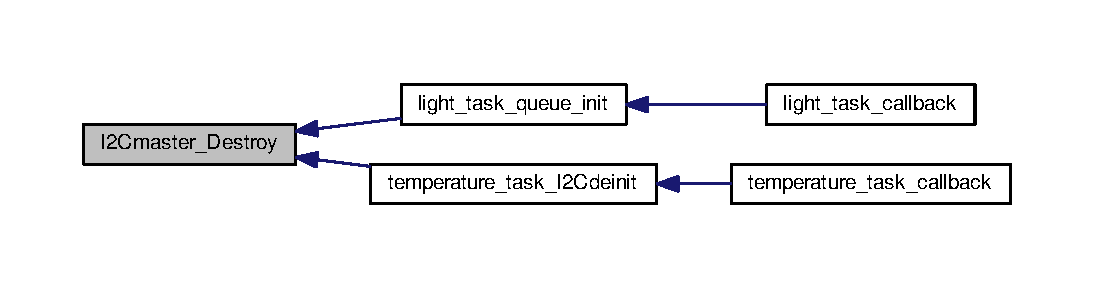
\includegraphics[width=350pt]{my__i2c_8h_a15136dcc397f046d0a000a781d060139_icgraph}
\end{center}
\end{figure}


\index{my\+\_\+i2c.\+h@{my\+\_\+i2c.\+h}!I2\+Cmaster\+\_\+\+Init@{I2\+Cmaster\+\_\+\+Init}}
\index{I2\+Cmaster\+\_\+\+Init@{I2\+Cmaster\+\_\+\+Init}!my\+\_\+i2c.\+h@{my\+\_\+i2c.\+h}}
\subsubsection[{\texorpdfstring{I2\+Cmaster\+\_\+\+Init(\+I2\+C\+\_\+\+M\+A\+S\+T\+E\+R\+\_\+\+H\+A\+N\+D\+L\+E\+\_\+\+T $\ast$handle)}{I2Cmaster_Init(I2C_MASTER_HANDLE_T *handle)}}]{\setlength{\rightskip}{0pt plus 5cm}int I2\+Cmaster\+\_\+\+Init (
\begin{DoxyParamCaption}
\item[{{\bf I2\+C\+\_\+\+M\+A\+S\+T\+E\+R\+\_\+\+H\+A\+N\+D\+L\+E\+\_\+T} $\ast$}]{handle}
\end{DoxyParamCaption}
)}\hypertarget{my__i2c_8h_acea2b6a0875bf63a179959a46b3cdf7d}{}\label{my__i2c_8h_acea2b6a0875bf63a179959a46b3cdf7d}


Inits the I2C master handle There is an internal state of the context which is maintained which gets updated with every init call Internal context goes to N\+U\+LL is error in init This context points to the new handle that is passed as the parameter. 


\begin{DoxyParams}{Parameters}
{\em handle} & \\
\hline
\end{DoxyParams}
\begin{DoxyReturn}{Returns}
int S\+U\+C\+C\+E\+SS=0 and E\+R\+R\+OR =-\/1 
\end{DoxyReturn}

\begin{DoxyCode}
26 \{
27     \textcolor{keywordtype}{int} ret = 0;
28     \textcolor{keywordflow}{if}(pthread\_mutex\_lock(&init\_destroy\_lock))
29         \textcolor{keywordflow}{return} -1;
30     \textcolor{keywordflow}{if}(NULL != internal\_master\_handle)
31     \{
32         handle = internal\_master\_handle;
33         ret =  0;
34     \}
35     \textcolor{keywordflow}{else} \textcolor{keywordflow}{if}(handle)
36     \{
37         handle->i2c\_context = mraa\_i2c\_init\_raw(BB\_I2C\_BUS\_2);
38         \textcolor{comment}{/* internal i2c context failed to init */}
39         \textcolor{keywordflow}{if}(NULL == handle->i2c\_context)
40         \{
41             internal\_master\_handle = NULL;
42             ret = -1;
43         \}
44         \textcolor{comment}{/* If spinlock init fails */}
45         \textcolor{keywordflow}{else} \textcolor{keywordflow}{if}( -1 == pthread\_spin\_init(&handle->handle\_lock, PTHREAD\_PROCESS\_PRIVATE))
46         \{
47             internal\_master\_handle = NULL;
48             mraa\_i2c\_stop(handle->i2c\_context);
49             ret = -1;
50         \}
51         \textcolor{comment}{/* Everyting goes as expected */}
52         \textcolor{keywordflow}{else}
53         \{
54             internal\_master\_handle = handle;
55             ret = 0;
56         \}
57     \}
58     \textcolor{comment}{/* If handle is null */}
59     \textcolor{keywordflow}{else}
60         ret = -1;
61 
62     \textcolor{keywordflow}{if}(pthread\_mutex\_unlock(&init\_destroy\_lock))
63         \textcolor{keywordflow}{return} -1;
64 
65     \textcolor{keywordflow}{return} ret;
66 \}
\end{DoxyCode}


Here is the caller graph for this function\+:
\nopagebreak
\begin{figure}[H]
\begin{center}
\leavevmode
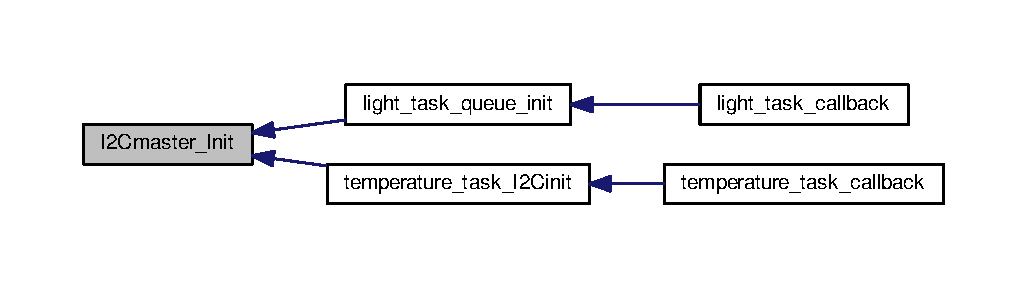
\includegraphics[width=350pt]{my__i2c_8h_acea2b6a0875bf63a179959a46b3cdf7d_icgraph}
\end{center}
\end{figure}


\index{my\+\_\+i2c.\+h@{my\+\_\+i2c.\+h}!I2\+Cmaster\+\_\+read\+\_\+byte@{I2\+Cmaster\+\_\+read\+\_\+byte}}
\index{I2\+Cmaster\+\_\+read\+\_\+byte@{I2\+Cmaster\+\_\+read\+\_\+byte}!my\+\_\+i2c.\+h@{my\+\_\+i2c.\+h}}
\subsubsection[{\texorpdfstring{I2\+Cmaster\+\_\+read\+\_\+byte(uint8\+\_\+t slave\+\_\+addr, uint8\+\_\+t reg\+\_\+addr, uint8\+\_\+t $\ast$data)}{I2Cmaster_read_byte(uint8_t slave_addr, uint8_t reg_addr, uint8_t *data)}}]{\setlength{\rightskip}{0pt plus 5cm}int I2\+Cmaster\+\_\+read\+\_\+byte (
\begin{DoxyParamCaption}
\item[{uint8\+\_\+t}]{slave\+\_\+addr, }
\item[{uint8\+\_\+t}]{reg\+\_\+addr, }
\item[{uint8\+\_\+t $\ast$}]{data}
\end{DoxyParamCaption}
)}\hypertarget{my__i2c_8h_a8024ad1f3558034ee998758f45d456d9}{}\label{my__i2c_8h_a8024ad1f3558034ee998758f45d456d9}

\begin{DoxyParams}{Parameters}
{\em slave\+\_\+addr} & \\
\hline
{\em reg\+\_\+addr} & \\
\hline
{\em data} & \\
\hline
\end{DoxyParams}
\begin{DoxyReturn}{Returns}
int 
\end{DoxyReturn}

\begin{DoxyCode}
181 \{
182     \textcolor{keywordflow}{if}(NULL == internal\_master\_handle)
183     \{
184         \textcolor{keywordflow}{return} -1;
185     \}
186 
187     pthread\_spin\_lock(&internal\_master\_handle->handle\_lock);
188 
189     mraa\_result\_t ret =  mraa\_i2c\_address(internal\_master\_handle->i2c\_context, slave\_addr);
190     \textcolor{keywordflow}{if}(0 == ret)
191     \{   
192         ret = mraa\_i2c\_read\_byte\_data(internal\_master\_handle->i2c\_context, reg\_addr);
193         (ret != -1) ? *data  = ret, ret = 0 : 0; 
194     \}
195 
196     pthread\_spin\_unlock(&internal\_master\_handle->handle\_lock);
197 
198     \textcolor{keywordflow}{return} ret;
199 
200 \}
\end{DoxyCode}


Here is the caller graph for this function\+:
\nopagebreak
\begin{figure}[H]
\begin{center}
\leavevmode
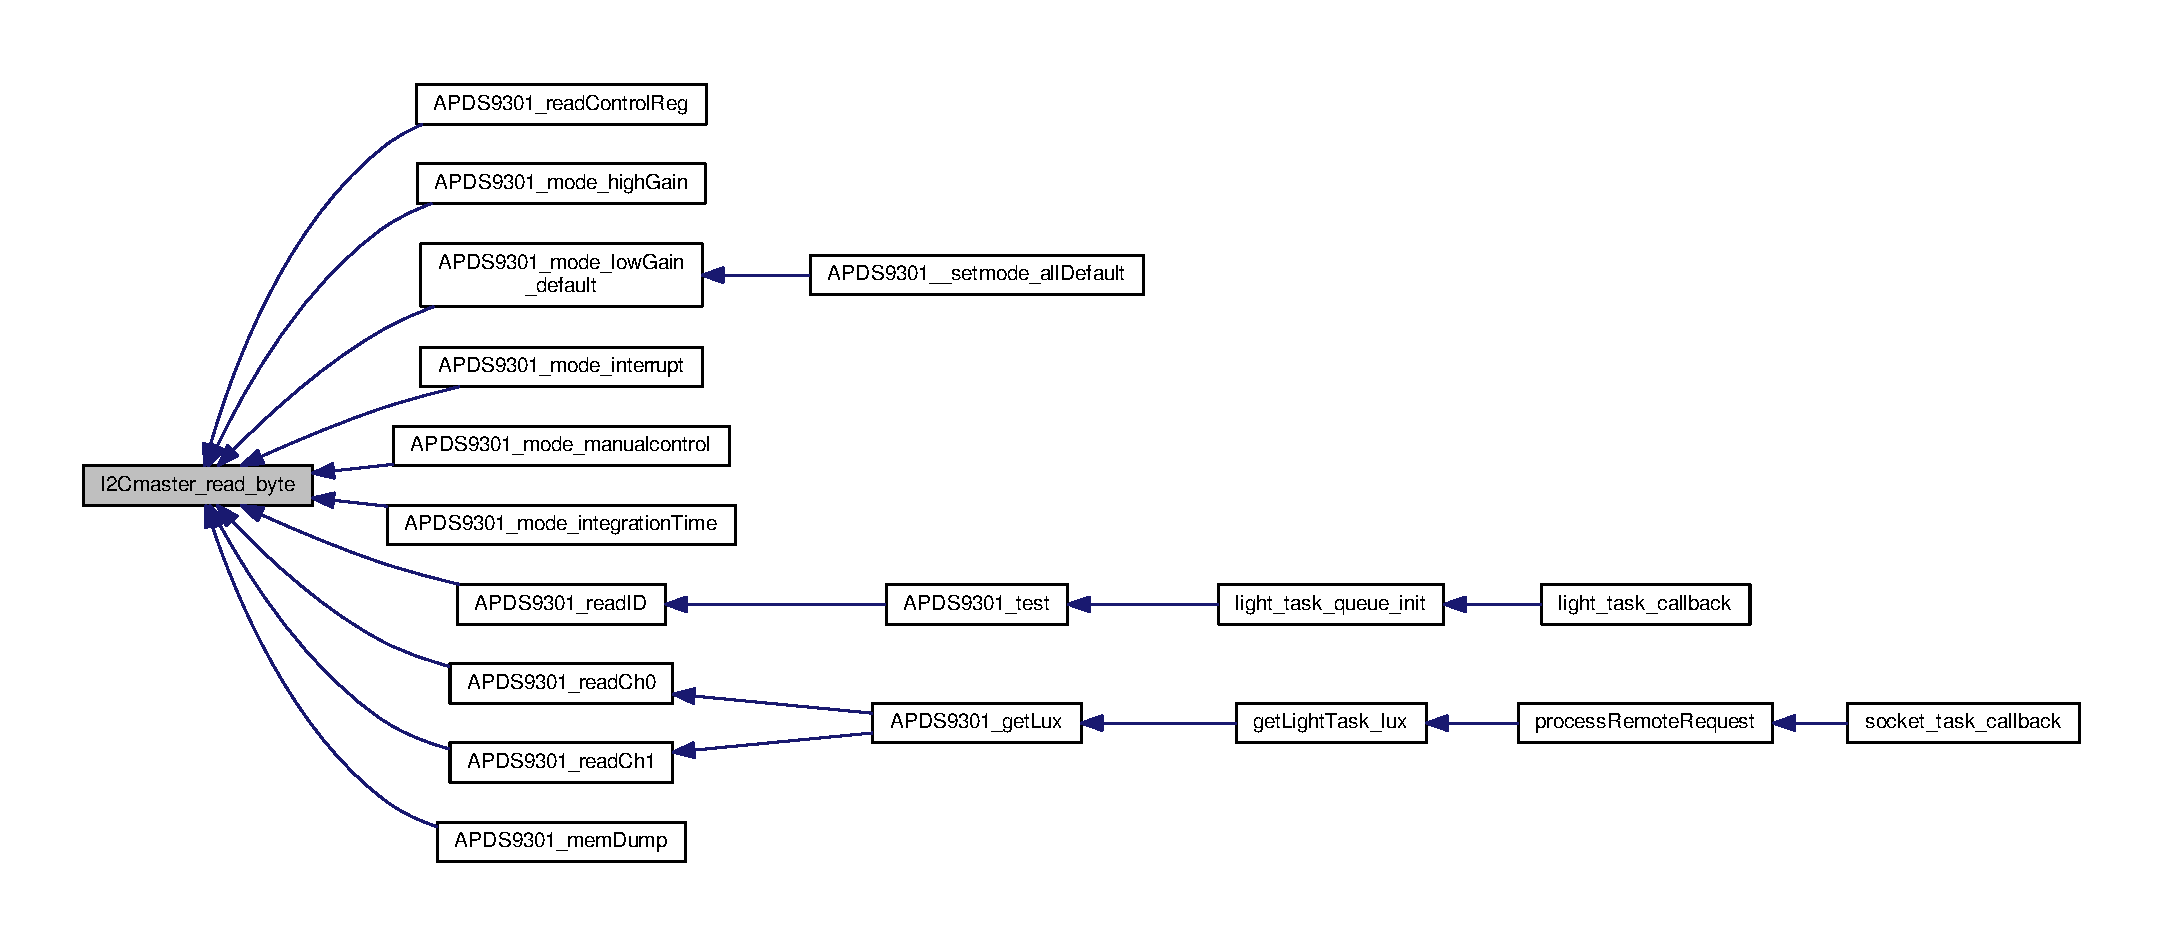
\includegraphics[width=350pt]{my__i2c_8h_a8024ad1f3558034ee998758f45d456d9_icgraph}
\end{center}
\end{figure}


\index{my\+\_\+i2c.\+h@{my\+\_\+i2c.\+h}!I2\+Cmaster\+\_\+read\+\_\+bytes@{I2\+Cmaster\+\_\+read\+\_\+bytes}}
\index{I2\+Cmaster\+\_\+read\+\_\+bytes@{I2\+Cmaster\+\_\+read\+\_\+bytes}!my\+\_\+i2c.\+h@{my\+\_\+i2c.\+h}}
\subsubsection[{\texorpdfstring{I2\+Cmaster\+\_\+read\+\_\+bytes(uint8\+\_\+t slave\+\_\+addr, uint8\+\_\+t reg\+\_\+addr, uint8\+\_\+t $\ast$data, size\+\_\+t len)}{I2Cmaster_read_bytes(uint8_t slave_addr, uint8_t reg_addr, uint8_t *data, size_t len)}}]{\setlength{\rightskip}{0pt plus 5cm}int I2\+Cmaster\+\_\+read\+\_\+bytes (
\begin{DoxyParamCaption}
\item[{uint8\+\_\+t}]{slave\+\_\+addr, }
\item[{uint8\+\_\+t}]{reg\+\_\+addr, }
\item[{uint8\+\_\+t $\ast$}]{data, }
\item[{size\+\_\+t}]{len}
\end{DoxyParamCaption}
)}\hypertarget{my__i2c_8h_ab25650a9cf74e65561b1fced3555f36c}{}\label{my__i2c_8h_ab25650a9cf74e65561b1fced3555f36c}

\begin{DoxyParams}{Parameters}
{\em slave\+\_\+addr} & \\
\hline
{\em reg\+\_\+addr} & \\
\hline
{\em data} & \\
\hline
{\em len} & \\
\hline
\end{DoxyParams}
\begin{DoxyReturn}{Returns}
int 
\end{DoxyReturn}

\begin{DoxyCode}
203 \{
204     \textcolor{keywordflow}{if}(NULL == internal\_master\_handle)
205     \{
206         \textcolor{keywordflow}{return} -1;
207     \}
208 
209     pthread\_spin\_lock(&internal\_master\_handle->handle\_lock);
210 
211     mraa\_result\_t ret =  mraa\_i2c\_address(internal\_master\_handle->i2c\_context, slave\_addr);
212     \textcolor{keywordflow}{if}(0 == ret)
213     \{   
214         ret = mraa\_i2c\_read\_bytes\_data(internal\_master\_handle->i2c\_context, reg\_addr, data , len);
215         (ret == len) ? ret = 0 : 0; 
216     \}
217 
218     pthread\_spin\_unlock(&internal\_master\_handle->handle\_lock);
219 
220     \textcolor{keywordflow}{return} ret;
221 \}
\end{DoxyCode}


Here is the caller graph for this function\+:
\nopagebreak
\begin{figure}[H]
\begin{center}
\leavevmode
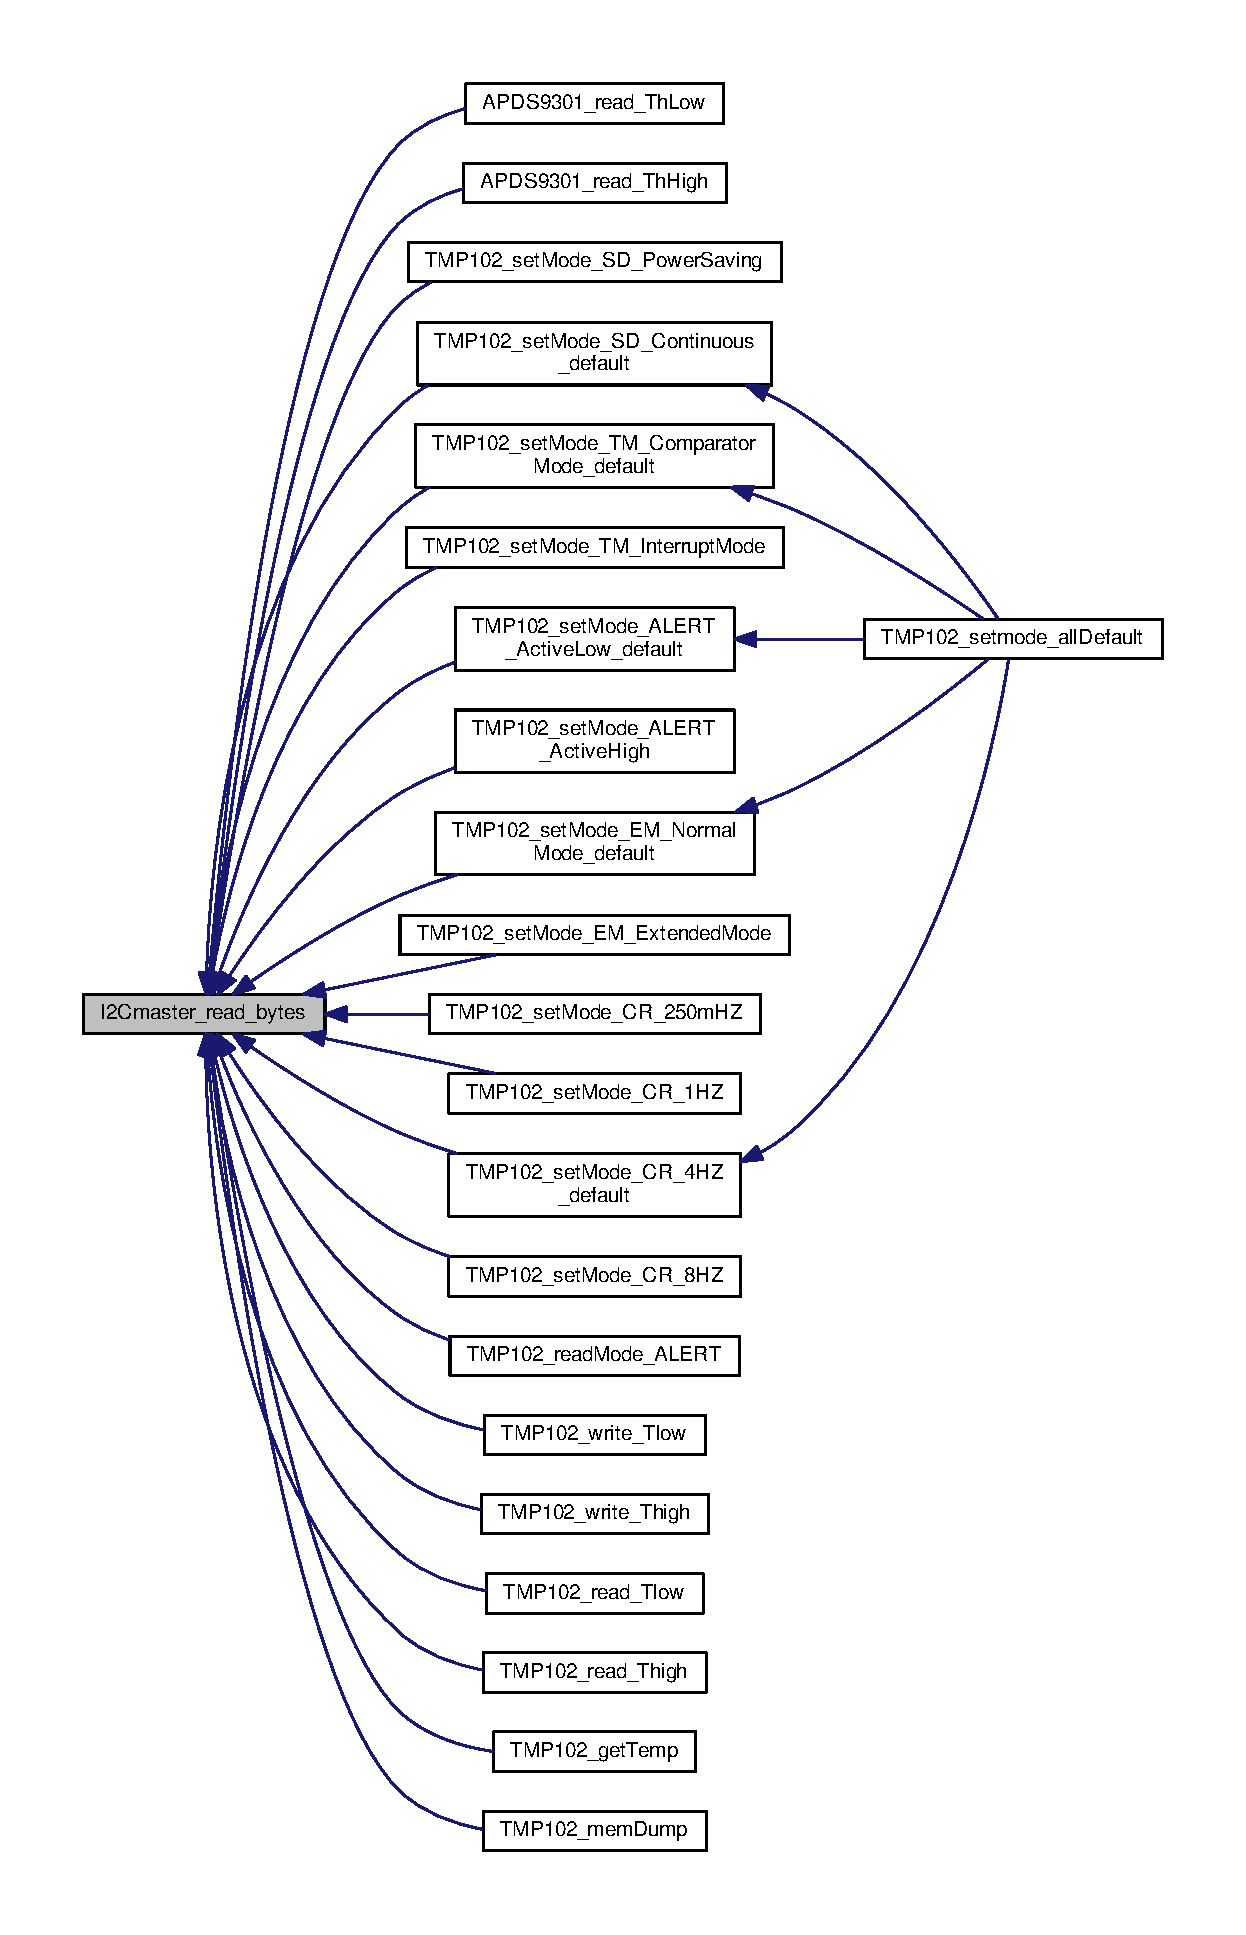
\includegraphics[width=350pt]{my__i2c_8h_ab25650a9cf74e65561b1fced3555f36c_icgraph}
\end{center}
\end{figure}


\index{my\+\_\+i2c.\+h@{my\+\_\+i2c.\+h}!I2\+Cmaster\+\_\+write@{I2\+Cmaster\+\_\+write}}
\index{I2\+Cmaster\+\_\+write@{I2\+Cmaster\+\_\+write}!my\+\_\+i2c.\+h@{my\+\_\+i2c.\+h}}
\subsubsection[{\texorpdfstring{I2\+Cmaster\+\_\+write(uint8\+\_\+t slave\+\_\+addr, uint8\+\_\+t reg\+\_\+addr)}{I2Cmaster_write(uint8_t slave_addr, uint8_t reg_addr)}}]{\setlength{\rightskip}{0pt plus 5cm}int I2\+Cmaster\+\_\+write (
\begin{DoxyParamCaption}
\item[{uint8\+\_\+t}]{slave\+\_\+addr, }
\item[{uint8\+\_\+t}]{reg\+\_\+addr}
\end{DoxyParamCaption}
)}\hypertarget{my__i2c_8h_af92cf5a5d893ef9bbf6b4ee6de0b0ef8}{}\label{my__i2c_8h_af92cf5a5d893ef9bbf6b4ee6de0b0ef8}


Writes a byte/pointer register to the slave. 


\begin{DoxyParams}{Parameters}
{\em slave\+\_\+addr} & \\
\hline
{\em reg\+\_\+addr} & \\
\hline
\end{DoxyParams}
\begin{DoxyReturn}{Returns}
int 
\end{DoxyReturn}

\begin{DoxyCode}
133 \{
134     \textcolor{keywordflow}{if}(NULL == internal\_master\_handle)
135     \{
136         \textcolor{keywordflow}{return} -1;
137     \}
138 
139     pthread\_spin\_lock(&internal\_master\_handle->handle\_lock);
140 
141     mraa\_result\_t ret =  mraa\_i2c\_address(internal\_master\_handle->i2c\_context, slave\_addr);
142     \textcolor{keywordflow}{if}(0 == ret)
143     \{   
144         ret = mraa\_i2c\_write\_byte(internal\_master\_handle->i2c\_context, reg\_addr);
145     \}
146 
147     pthread\_spin\_unlock(&internal\_master\_handle->handle\_lock);
148 
149     \textcolor{keywordflow}{return} ret;
150 \}
\end{DoxyCode}


Here is the caller graph for this function\+:
\nopagebreak
\begin{figure}[H]
\begin{center}
\leavevmode
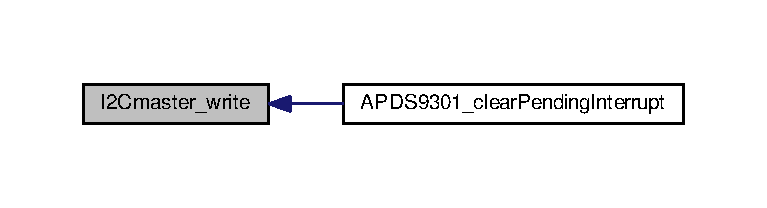
\includegraphics[width=350pt]{my__i2c_8h_af92cf5a5d893ef9bbf6b4ee6de0b0ef8_icgraph}
\end{center}
\end{figure}


\index{my\+\_\+i2c.\+h@{my\+\_\+i2c.\+h}!I2\+Cmaster\+\_\+write\+\_\+byte@{I2\+Cmaster\+\_\+write\+\_\+byte}}
\index{I2\+Cmaster\+\_\+write\+\_\+byte@{I2\+Cmaster\+\_\+write\+\_\+byte}!my\+\_\+i2c.\+h@{my\+\_\+i2c.\+h}}
\subsubsection[{\texorpdfstring{I2\+Cmaster\+\_\+write\+\_\+byte(uint8\+\_\+t slave\+\_\+addr, uint8\+\_\+t reg\+\_\+addr, uint8\+\_\+t data)}{I2Cmaster_write_byte(uint8_t slave_addr, uint8_t reg_addr, uint8_t data)}}]{\setlength{\rightskip}{0pt plus 5cm}int I2\+Cmaster\+\_\+write\+\_\+byte (
\begin{DoxyParamCaption}
\item[{uint8\+\_\+t}]{slave\+\_\+addr, }
\item[{uint8\+\_\+t}]{reg\+\_\+addr, }
\item[{uint8\+\_\+t}]{data}
\end{DoxyParamCaption}
)}\hypertarget{my__i2c_8h_a202be1d68320e3ba93c759821ba2f695}{}\label{my__i2c_8h_a202be1d68320e3ba93c759821ba2f695}

\begin{DoxyParams}{Parameters}
{\em slave\+\_\+addr} & \\
\hline
{\em reg\+\_\+addr} & \\
\hline
{\em data} & \\
\hline
\end{DoxyParams}
\begin{DoxyReturn}{Returns}
int 
\end{DoxyReturn}

\begin{DoxyCode}
113 \{
114     \textcolor{keywordflow}{if}(NULL == internal\_master\_handle)
115     \{
116         \textcolor{keywordflow}{return} -1;
117     \}
118 
119     pthread\_spin\_lock(&internal\_master\_handle->handle\_lock);
120 
121     mraa\_result\_t ret =  mraa\_i2c\_address(internal\_master\_handle->i2c\_context, slave\_addr);
122     \textcolor{keywordflow}{if}(0 == ret)
123     \{   
124         ret = mraa\_i2c\_write\_byte\_data(internal\_master\_handle->i2c\_context, data, reg\_addr);
125     \}
126 
127     pthread\_spin\_unlock(&internal\_master\_handle->handle\_lock);
128 
129     \textcolor{keywordflow}{return} ret;
130 \}
\end{DoxyCode}


Here is the caller graph for this function\+:
\nopagebreak
\begin{figure}[H]
\begin{center}
\leavevmode
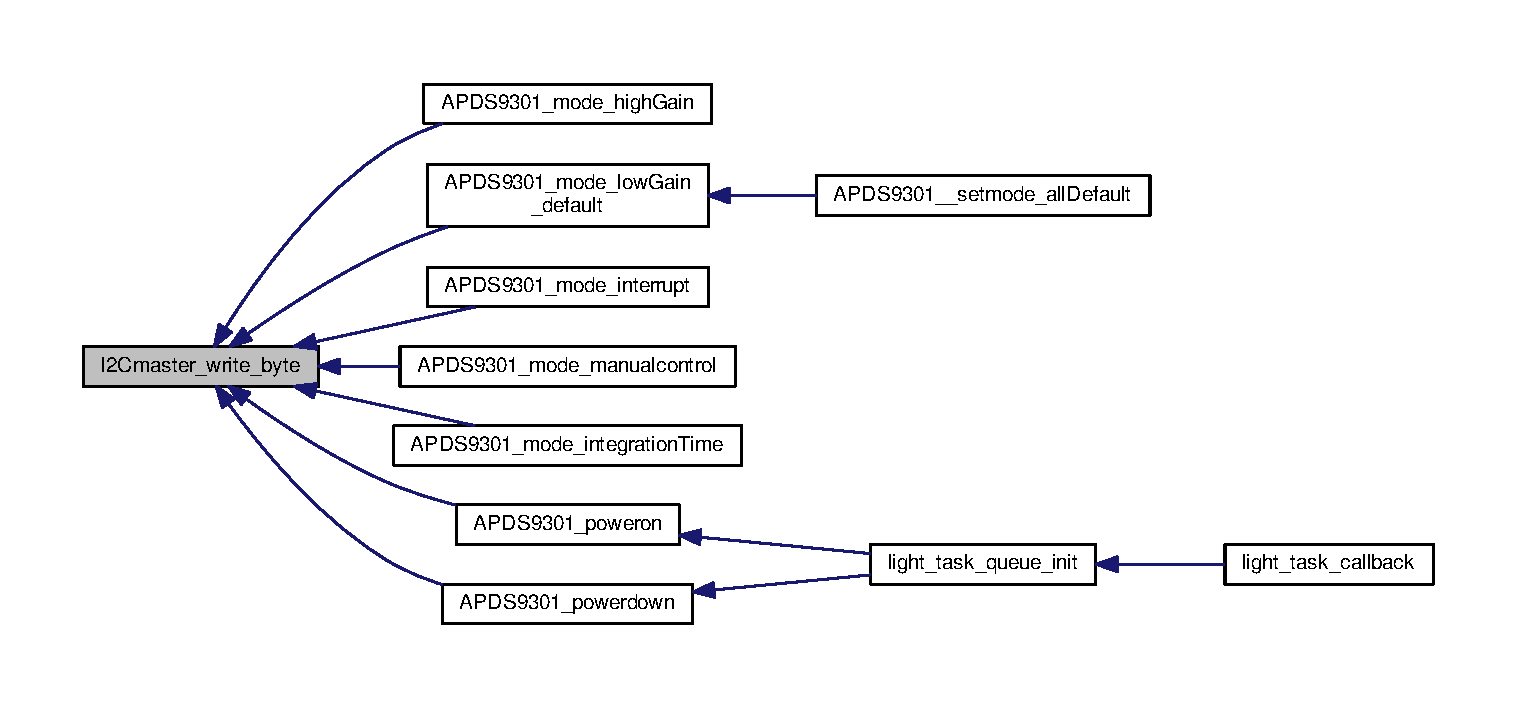
\includegraphics[width=350pt]{my__i2c_8h_a202be1d68320e3ba93c759821ba2f695_icgraph}
\end{center}
\end{figure}


\index{my\+\_\+i2c.\+h@{my\+\_\+i2c.\+h}!I2\+Cmaster\+\_\+write\+\_\+bytes@{I2\+Cmaster\+\_\+write\+\_\+bytes}}
\index{I2\+Cmaster\+\_\+write\+\_\+bytes@{I2\+Cmaster\+\_\+write\+\_\+bytes}!my\+\_\+i2c.\+h@{my\+\_\+i2c.\+h}}
\subsubsection[{\texorpdfstring{I2\+Cmaster\+\_\+write\+\_\+bytes(uint8\+\_\+t slave\+\_\+addr, uint8\+\_\+t reg\+\_\+addr, uint8\+\_\+t $\ast$data, size\+\_\+t len)}{I2Cmaster_write_bytes(uint8_t slave_addr, uint8_t reg_addr, uint8_t *data, size_t len)}}]{\setlength{\rightskip}{0pt plus 5cm}int I2\+Cmaster\+\_\+write\+\_\+bytes (
\begin{DoxyParamCaption}
\item[{uint8\+\_\+t}]{slave\+\_\+addr, }
\item[{uint8\+\_\+t}]{reg\+\_\+addr, }
\item[{uint8\+\_\+t $\ast$}]{data, }
\item[{size\+\_\+t}]{len}
\end{DoxyParamCaption}
)}\hypertarget{my__i2c_8h_a3a48cfc824f745c311bc081479ee6b9b}{}\label{my__i2c_8h_a3a48cfc824f745c311bc081479ee6b9b}

\begin{DoxyParams}{Parameters}
{\em slave\+\_\+addr} & \\
\hline
{\em reg\+\_\+addr} & \\
\hline
{\em data} & \\
\hline
{\em len} & \\
\hline
\end{DoxyParams}
\begin{DoxyReturn}{Returns}
int 
\end{DoxyReturn}
\index{my\+\_\+i2c.\+h@{my\+\_\+i2c.\+h}!I2\+Cmaster\+\_\+write\+\_\+word@{I2\+Cmaster\+\_\+write\+\_\+word}}
\index{I2\+Cmaster\+\_\+write\+\_\+word@{I2\+Cmaster\+\_\+write\+\_\+word}!my\+\_\+i2c.\+h@{my\+\_\+i2c.\+h}}
\subsubsection[{\texorpdfstring{I2\+Cmaster\+\_\+write\+\_\+word(uint8\+\_\+t slave\+\_\+addr, uint8\+\_\+t reg\+\_\+addr, uint16\+\_\+t data, uint8\+\_\+t lsb\+\_\+first)}{I2Cmaster_write_word(uint8_t slave_addr, uint8_t reg_addr, uint16_t data, uint8_t lsb_first)}}]{\setlength{\rightskip}{0pt plus 5cm}int I2\+Cmaster\+\_\+write\+\_\+word (
\begin{DoxyParamCaption}
\item[{uint8\+\_\+t}]{slave\+\_\+addr, }
\item[{uint8\+\_\+t}]{reg\+\_\+addr, }
\item[{uint16\+\_\+t}]{data, }
\item[{uint8\+\_\+t}]{lsb\+\_\+first}
\end{DoxyParamCaption}
)}\hypertarget{my__i2c_8h_a19c6244da5ea2d4e65a25001582498c8}{}\label{my__i2c_8h_a19c6244da5ea2d4e65a25001582498c8}

\begin{DoxyParams}{Parameters}
{\em slave\+\_\+addr} & \\
\hline
{\em reg\+\_\+addr} & \\
\hline
{\em data} & \\
\hline
{\em lsb\+\_\+first} & \\
\hline
\end{DoxyParams}
\begin{DoxyReturn}{Returns}
int 
\end{DoxyReturn}

\begin{DoxyCode}
154 \{
155     \textcolor{keywordflow}{if}(NULL == internal\_master\_handle)
156     \{
157         \textcolor{keywordflow}{return} -1;
158     \}
159     
160     \textcolor{keywordflow}{if}(lsb\_first)
161     \{
162         data = ( ((data & 0xF0)>>4)| ((data &0x0F)<<4) ); 
163     \}
164 
165     pthread\_spin\_lock(&internal\_master\_handle->handle\_lock);
166 
167     mraa\_result\_t ret =  mraa\_i2c\_address(internal\_master\_handle->i2c\_context, slave\_addr);
168     \textcolor{keywordflow}{if}(0 == ret)
169     \{   
170         ret = mraa\_i2c\_write\_word\_data(internal\_master\_handle->i2c\_context, data, reg\_addr);
171     \}
172 
173     pthread\_spin\_unlock(&internal\_master\_handle->handle\_lock);
174 
175     \textcolor{keywordflow}{return} ret;
176 
177 \}
\end{DoxyCode}


Here is the caller graph for this function\+:
\nopagebreak
\begin{figure}[H]
\begin{center}
\leavevmode
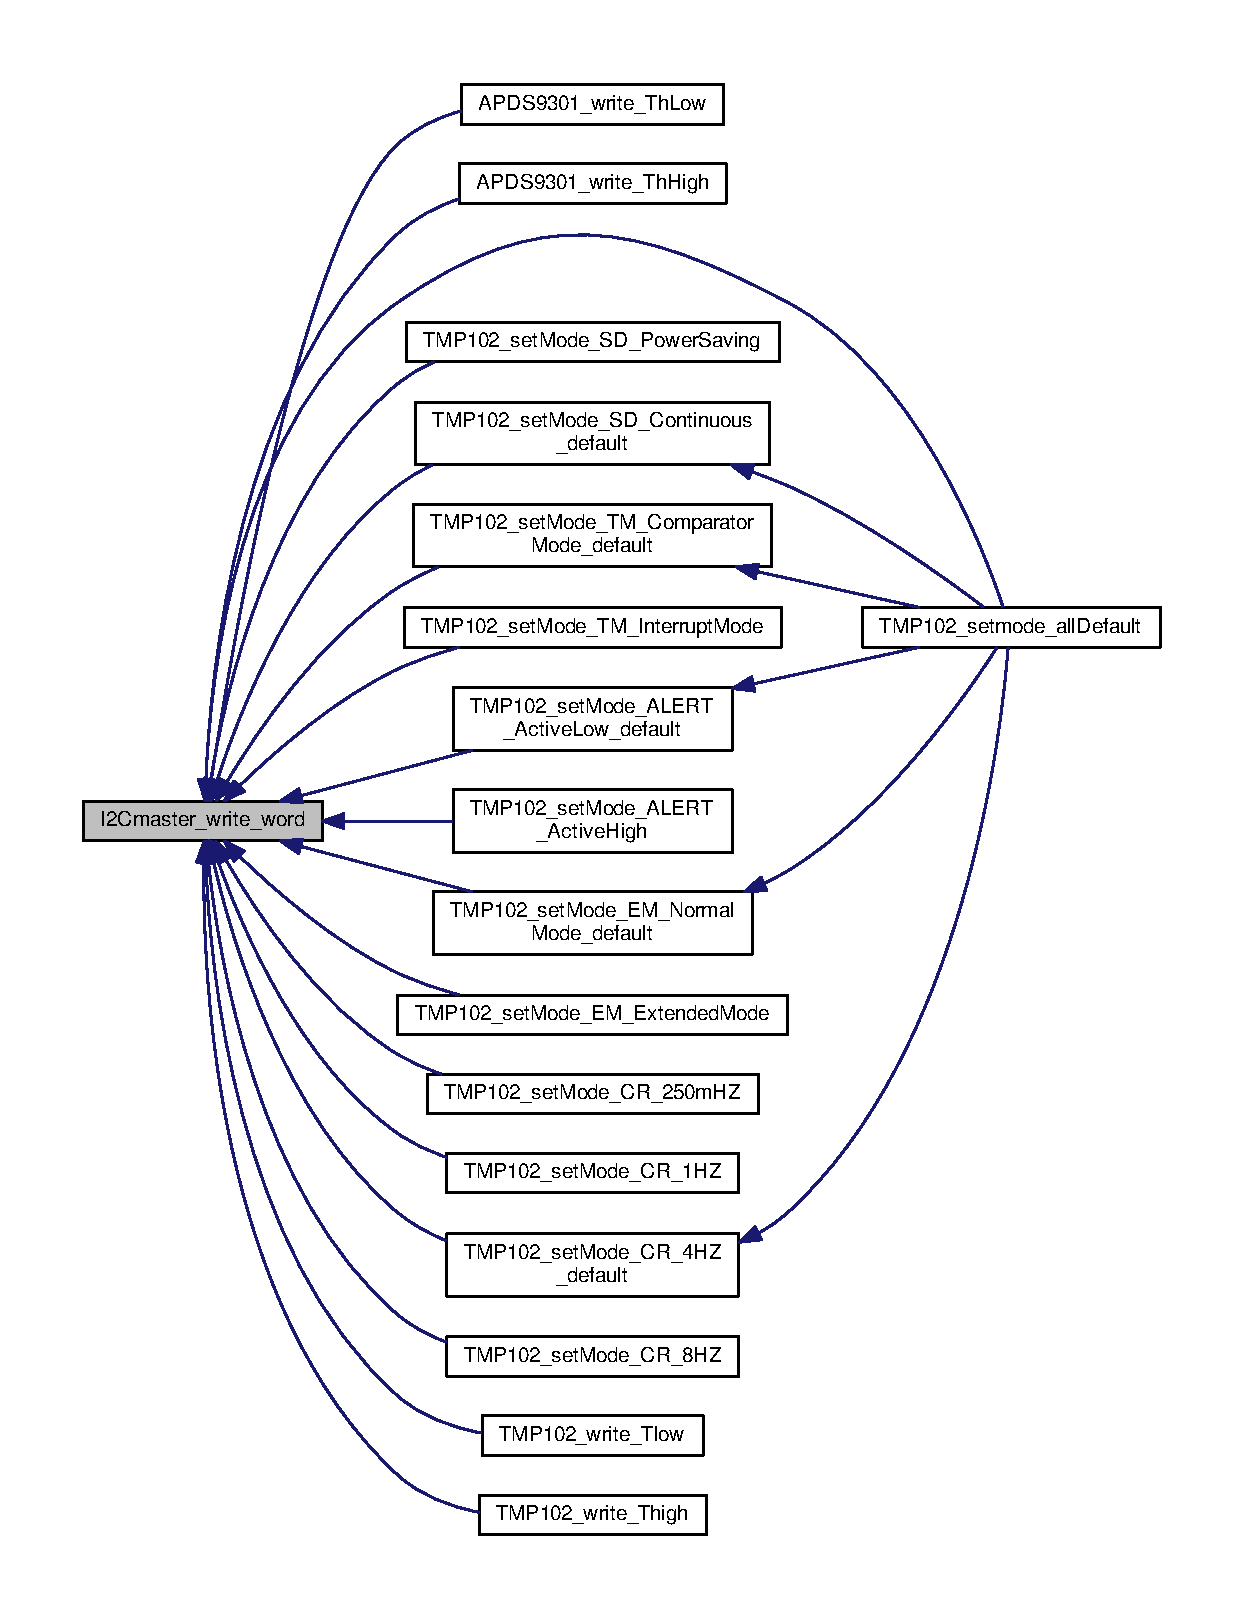
\includegraphics[width=350pt]{my__i2c_8h_a19c6244da5ea2d4e65a25001582498c8_icgraph}
\end{center}
\end{figure}


\index{my\+\_\+i2c.\+h@{my\+\_\+i2c.\+h}!print\+Error\+Code@{print\+Error\+Code}}
\index{print\+Error\+Code@{print\+Error\+Code}!my\+\_\+i2c.\+h@{my\+\_\+i2c.\+h}}
\subsubsection[{\texorpdfstring{print\+Error\+Code(int error\+Code)}{printErrorCode(int errorCode)}}]{\setlength{\rightskip}{0pt plus 5cm}void print\+Error\+Code (
\begin{DoxyParamCaption}
\item[{int}]{error\+Code}
\end{DoxyParamCaption}
)}\hypertarget{my__i2c_8h_a24206855ca77b181de1cfbe8e9e5051a}{}\label{my__i2c_8h_a24206855ca77b181de1cfbe8e9e5051a}


Prints the error code string to stdout. 


\begin{DoxyParams}{Parameters}
{\em error\+Code} & \\
\hline
\end{DoxyParams}

\begin{DoxyCode}
18 \{
19     \textcolor{comment}{//#define VERBOSE}
20 \textcolor{preprocessor}{    #ifdef VERBOSE}
21     mraa\_result\_print(errorCode);
22 \textcolor{preprocessor}{    #endif}
23 \}
\end{DoxyCode}


Here is the caller graph for this function\+:
\nopagebreak
\begin{figure}[H]
\begin{center}
\leavevmode
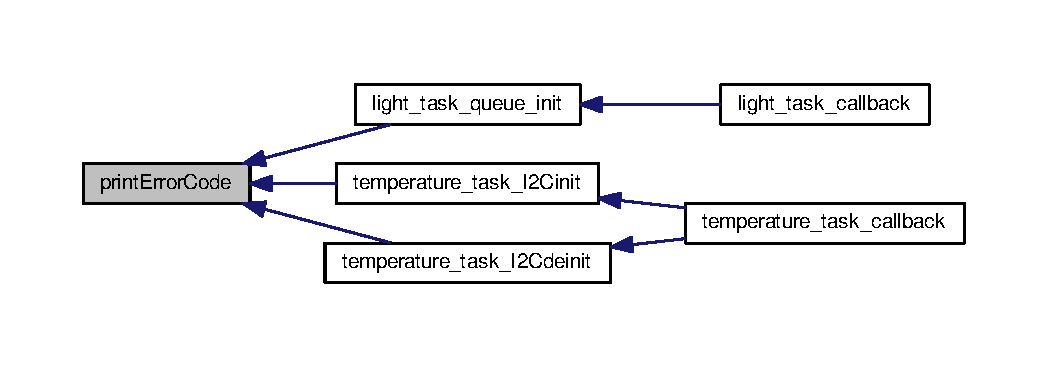
\includegraphics[width=350pt]{my__i2c_8h_a24206855ca77b181de1cfbe8e9e5051a_icgraph}
\end{center}
\end{figure}



\hypertarget{tmp102__sensor_8h}{}\section{/home/gunj/repos/\+E\+C\+E\+N-\/5013/\+Project1/include/\+Beagle\+Bone/tmp102\+\_\+sensor.h File Reference}
\label{tmp102__sensor_8h}\index{/home/gunj/repos/\+E\+C\+E\+N-\/5013/\+Project1/include/\+Beagle\+Bone/tmp102\+\_\+sensor.\+h@{/home/gunj/repos/\+E\+C\+E\+N-\/5013/\+Project1/include/\+Beagle\+Bone/tmp102\+\_\+sensor.\+h}}
This graph shows which files directly or indirectly include this file\+:\nopagebreak
\begin{figure}[H]
\begin{center}
\leavevmode
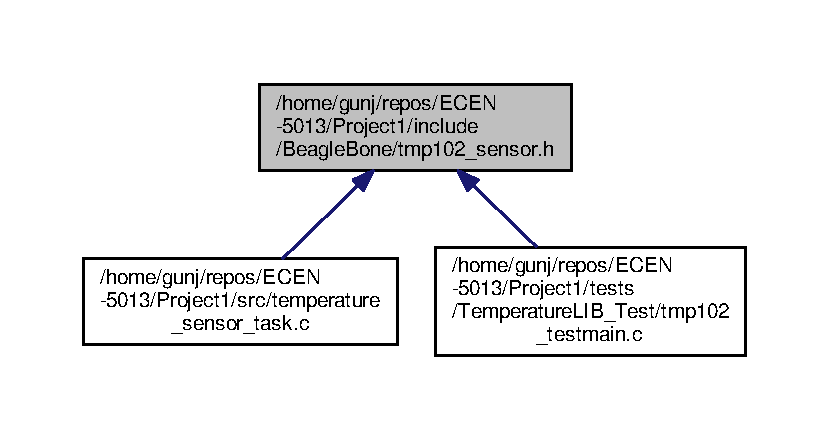
\includegraphics[width=350pt]{tmp102__sensor_8h__dep__incl}
\end{center}
\end{figure}
\subsection*{Data Structures}
\begin{DoxyCompactItemize}
\item 
struct \hyperlink{structTMP102__CONFIG__REG__SETTINGS__T}{T\+M\+P102\+\_\+\+C\+O\+N\+F\+I\+G\+\_\+\+R\+E\+G\+\_\+\+S\+E\+T\+T\+I\+N\+G\+S\+\_\+T}
\end{DoxyCompactItemize}
\subsection*{Macros}
\begin{DoxyCompactItemize}
\item 
\#define {\bfseries T\+M\+P102\+\_\+\+S\+L\+A\+V\+E\+\_\+\+A\+D\+DR}~(0x48)\hypertarget{tmp102__sensor_8h_a5092a6804ba3b3746307a370defbd886}{}\label{tmp102__sensor_8h_a5092a6804ba3b3746307a370defbd886}

\item 
\#define {\bfseries T\+M\+P102\+\_\+\+R\+E\+G\+\_\+\+T\+E\+M\+P\+E\+R\+A\+T\+U\+RE}~(0x00)\hypertarget{tmp102__sensor_8h_aea6533288f31ec0c0315dd54f929fee5}{}\label{tmp102__sensor_8h_aea6533288f31ec0c0315dd54f929fee5}

\item 
\#define {\bfseries T\+M\+P102\+\_\+\+R\+E\+G\+\_\+\+C\+O\+N\+F\+I\+G\+U\+R\+A\+T\+I\+ON}~(0x01)\hypertarget{tmp102__sensor_8h_ad0625a9e3e89c267c5060a3c01f34011}{}\label{tmp102__sensor_8h_ad0625a9e3e89c267c5060a3c01f34011}

\item 
\#define {\bfseries T\+M\+P102\+\_\+\+R\+E\+G\+\_\+\+T\+L\+OW}~(0x02)\hypertarget{tmp102__sensor_8h_a26f5d3c790581774f55998360b248769}{}\label{tmp102__sensor_8h_a26f5d3c790581774f55998360b248769}

\item 
\#define {\bfseries T\+M\+P102\+\_\+\+R\+E\+G\+\_\+\+T\+H\+I\+GH}~(0x03)\hypertarget{tmp102__sensor_8h_a2705c0ccf3404fffcf0f3566914f98ba}{}\label{tmp102__sensor_8h_a2705c0ccf3404fffcf0f3566914f98ba}

\item 
\#define {\bfseries T\+M\+P102\+\_\+\+C\+O\+N\+F\+I\+G\+\_\+\+SD}~(1)\hypertarget{tmp102__sensor_8h_a88a716e4fccaa747f3ff9c2ff98b3eec}{}\label{tmp102__sensor_8h_a88a716e4fccaa747f3ff9c2ff98b3eec}

\item 
\#define {\bfseries T\+M\+P102\+\_\+\+C\+O\+N\+F\+I\+G\+\_\+\+TM}~(1$<$$<$1)\hypertarget{tmp102__sensor_8h_abf3813bf9769e2d22bdc37e5e0e7b2f9}{}\label{tmp102__sensor_8h_abf3813bf9769e2d22bdc37e5e0e7b2f9}

\item 
\#define {\bfseries T\+M\+P102\+\_\+\+C\+O\+N\+F\+I\+G\+\_\+\+P\+OL}~(1$<$$<$2)\hypertarget{tmp102__sensor_8h_a008cb8f9704db90f09d4e4b2dd8c040b}{}\label{tmp102__sensor_8h_a008cb8f9704db90f09d4e4b2dd8c040b}

\item 
\#define {\bfseries T\+M\+P102\+\_\+\+C\+O\+N\+F\+I\+G\+\_\+\+EM}~(1$<$$<$12)\hypertarget{tmp102__sensor_8h_a5bba383a7572ce8264417e7f6426ce88}{}\label{tmp102__sensor_8h_a5bba383a7572ce8264417e7f6426ce88}

\item 
\#define {\bfseries T\+M\+P102\+\_\+\+C\+O\+N\+F\+I\+G\+\_\+\+AL}~(1$<$$<$13)\hypertarget{tmp102__sensor_8h_a6daed77089fc130171b75fb77dfb3661}{}\label{tmp102__sensor_8h_a6daed77089fc130171b75fb77dfb3661}

\item 
\#define {\bfseries T\+M\+P102\+\_\+\+C\+O\+N\+F\+I\+G\+\_\+\+CR}(x)~(x$<$$<$14)\hypertarget{tmp102__sensor_8h_a54602466d5eaacf584b283c626c06eb9}{}\label{tmp102__sensor_8h_a54602466d5eaacf584b283c626c06eb9}

\item 
\#define {\bfseries T\+M\+P102\+\_\+\+C\+O\+N\+F\+I\+G\+\_\+\+F\+A\+U\+L\+T\+B\+I\+TS}~(3$<$$<$3)              /$\ast$generates alert after 4 consecutive faults$\ast$/\hypertarget{tmp102__sensor_8h_a87bc9726a0037e6f8a3baf036a50cc34}{}\label{tmp102__sensor_8h_a87bc9726a0037e6f8a3baf036a50cc34}

\item 
\#define {\bfseries T\+M\+P102\+\_\+\+C\+O\+N\+F\+I\+G\+\_\+\+O\+N\+E\+S\+H\+O\+T\+\_\+\+CR}~(1$<$7)              /$\ast$saves power between conversions when 1$\ast$/\hypertarget{tmp102__sensor_8h_aff0b28b78374e0658675e4d38ef62d2e}{}\label{tmp102__sensor_8h_aff0b28b78374e0658675e4d38ef62d2e}

\item 
\#define {\bfseries T\+M\+P102\+\_\+\+C\+O\+N\+F\+I\+G\+\_\+\+D\+E\+F\+A\+U\+L\+T\+\_\+\+A\+S\+S\+I\+GN}
\item 
\#define \hyperlink{tmp102__sensor_8h_ab79ca2cd8f6ac2c6edb369185a4ec9e2}{T\+M\+P102\+\_\+get\+Temp\+\_\+\+Celcius}(p\+\_\+temp)~\hyperlink{tmp102__sensor_8h_a847d6333b56e33f815bb5e1101056e42}{T\+M\+P102\+\_\+get\+Temp}(p\+\_\+temp, C\+E\+L\+C\+I\+US)\hypertarget{tmp102__sensor_8h_ab79ca2cd8f6ac2c6edb369185a4ec9e2}{}\label{tmp102__sensor_8h_ab79ca2cd8f6ac2c6edb369185a4ec9e2}

\begin{DoxyCompactList}\small\item\em Abstracted macros for different units. \end{DoxyCompactList}\item 
\#define {\bfseries T\+M\+P102\+\_\+get\+Temp\+\_\+\+Kelvin}(p\+\_\+temp)~\hyperlink{tmp102__sensor_8h_a847d6333b56e33f815bb5e1101056e42}{T\+M\+P102\+\_\+get\+Temp}(p\+\_\+temp, K\+E\+L\+V\+IN)\hypertarget{tmp102__sensor_8h_a164eefae884728c9725a07253de91b34}{}\label{tmp102__sensor_8h_a164eefae884728c9725a07253de91b34}

\item 
\#define {\bfseries T\+M\+P102\+\_\+get\+Temp\+\_\+\+Fahren}(p\+\_\+temp)~\hyperlink{tmp102__sensor_8h_a847d6333b56e33f815bb5e1101056e42}{T\+M\+P102\+\_\+get\+Temp}(p\+\_\+temp, F\+A\+H\+R\+EN)\hypertarget{tmp102__sensor_8h_a614c139921346bfb450e1e51c5239e75}{}\label{tmp102__sensor_8h_a614c139921346bfb450e1e51c5239e75}

\end{DoxyCompactItemize}
\subsection*{Typedefs}
\begin{DoxyCompactItemize}
\item 
typedef enum temperature\+\_\+unit {\bfseries T\+E\+M\+P\+E\+R\+A\+T\+U\+R\+E\+\_\+\+U\+N\+I\+T\+\_\+T}\hypertarget{tmp102__sensor_8h_a2ffc14fbf10761dbe31056dc66d1986e}{}\label{tmp102__sensor_8h_a2ffc14fbf10761dbe31056dc66d1986e}

\end{DoxyCompactItemize}
\subsection*{Enumerations}
\begin{DoxyCompactItemize}
\item 
enum {\bfseries temperature\+\_\+unit} \{ {\bfseries C\+E\+L\+C\+I\+US} = 0, 
{\bfseries F\+A\+H\+R\+EN}, 
{\bfseries K\+E\+L\+V\+IN}
 \}\hypertarget{tmp102__sensor_8h_a97e99b5bf85609e1aa08fadbc777f26a}{}\label{tmp102__sensor_8h_a97e99b5bf85609e1aa08fadbc777f26a}

\end{DoxyCompactItemize}
\subsection*{Functions}
\begin{DoxyCompactItemize}
\item 
int {\bfseries T\+M\+P102\+\_\+set\+Mode} (\hyperlink{structTMP102__CONFIG__REG__SETTINGS__T}{T\+M\+P102\+\_\+\+C\+O\+N\+F\+I\+G\+\_\+\+R\+E\+G\+\_\+\+S\+E\+T\+T\+I\+N\+G\+S\+\_\+T} mode)\hypertarget{tmp102__sensor_8h_ae5d236342ee1df3c285e70ec22d9a48e}{}\label{tmp102__sensor_8h_ae5d236342ee1df3c285e70ec22d9a48e}

\item 
int \hyperlink{tmp102__sensor_8h_a4725fb3e4cf18de4220d6067a7dc5dd4}{T\+M\+P102\+\_\+setmode\+\_\+all\+Default} ()
\begin{DoxyCompactList}\small\item\em Brings back to default. \end{DoxyCompactList}\item 
uint16\+\_\+t $\ast$ \hyperlink{tmp102__sensor_8h_a1ea9cb5a6a2e798b33564f9142d7afa1}{T\+M\+P102\+\_\+mem\+Dump} ()
\begin{DoxyCompactList}\small\item\em Gives a memdump of 4 len. {\bfseries I\+MP} must free the address using return pointer. \end{DoxyCompactList}\item 
int \hyperlink{tmp102__sensor_8h_a847d6333b56e33f815bb5e1101056e42}{T\+M\+P102\+\_\+get\+Temp} (float $\ast$temp, T\+E\+M\+P\+E\+R\+A\+T\+U\+R\+E\+\_\+\+U\+N\+I\+T\+\_\+T unit)
\begin{DoxyCompactList}\small\item\em Gets the temperature value. \end{DoxyCompactList}\item 
int \hyperlink{tmp102__sensor_8h_a7d4d57387ef6a5db5bfc8d14a94d9ee4}{T\+M\+P102\+\_\+set\+Mode\+\_\+\+S\+D\+\_\+\+Power\+Saving} ()
\item 
int \hyperlink{tmp102__sensor_8h_a4309a30e9d006753c2cdd6f6c9af2650}{T\+M\+P102\+\_\+set\+Mode\+\_\+\+S\+D\+\_\+\+Continuous\+\_\+default} ()
\item 
int \hyperlink{tmp102__sensor_8h_a81c75dba63b6c0727ab602ea631b3a22}{T\+M\+P102\+\_\+set\+Mode\+\_\+\+T\+M\+\_\+\+Comparator\+Mode\+\_\+default} ()
\item 
int \hyperlink{tmp102__sensor_8h_a4386703b35277dc71be5cd9b57d0f3ce}{T\+M\+P102\+\_\+set\+Mode\+\_\+\+T\+M\+\_\+\+Interrupt\+Mode} ()
\item 
int \hyperlink{tmp102__sensor_8h_a899854f020db34f588f89adffcdc8433}{T\+M\+P102\+\_\+set\+Mode\+\_\+\+A\+L\+E\+R\+T\+\_\+\+Active\+Low\+\_\+default} ()
\item 
int \hyperlink{tmp102__sensor_8h_aa7438de8c6766d48b649e132cabf88e9}{T\+M\+P102\+\_\+set\+Mode\+\_\+\+A\+L\+E\+R\+T\+\_\+\+Active\+High} ()
\item 
int \hyperlink{tmp102__sensor_8h_aa96f470639b851a96f524ae6524dd266}{T\+M\+P102\+\_\+set\+Mode\+\_\+\+E\+M\+\_\+\+Normal\+Mode\+\_\+default} ()
\item 
int \hyperlink{tmp102__sensor_8h_a2df18183afad1339903fe59997aaf9a2}{T\+M\+P102\+\_\+set\+Mode\+\_\+\+E\+M\+\_\+\+Extended\+Mode} ()
\item 
int \hyperlink{tmp102__sensor_8h_a3f6277d742af4a10dcec568e84ad1d5d}{T\+M\+P102\+\_\+set\+Mode\+\_\+\+C\+R\+\_\+250m\+HZ} ()
\item 
int \hyperlink{tmp102__sensor_8h_a110d2f8672865d85670f2681e5dc9aed}{T\+M\+P102\+\_\+set\+Mode\+\_\+\+C\+R\+\_\+1\+HZ} ()
\item 
int \hyperlink{tmp102__sensor_8h_a6d24a33a5e009441edb99bd1a727afec}{T\+M\+P102\+\_\+set\+Mode\+\_\+\+C\+R\+\_\+4\+H\+Z\+\_\+default} ()
\item 
int \hyperlink{tmp102__sensor_8h_a031c7291b177515876ebb29d24dc97b4}{T\+M\+P102\+\_\+set\+Mode\+\_\+\+C\+R\+\_\+8\+HZ} ()
\item 
int \hyperlink{tmp102__sensor_8h_a98961eafa743b9a651a3cd2f3787f858}{T\+M\+P102\+\_\+read\+Mode\+\_\+\+A\+L\+E\+RT} (uint8\+\_\+t $\ast$al\+\_\+bit)
\item 
int \hyperlink{tmp102__sensor_8h_a6296f70167b1f662c7f9b56b15fe037c}{T\+M\+P102\+\_\+write\+\_\+\+Tlow} (float tlow\+\_\+C)
\item 
int \hyperlink{tmp102__sensor_8h_a32a4b8bbc5611a7ca967cdaaeb732ae1}{T\+M\+P102\+\_\+write\+\_\+\+Thigh} (float thigh\+\_\+C)
\item 
int \hyperlink{tmp102__sensor_8h_aa8531a04dcf776f0d81d190b384bfab5}{T\+M\+P102\+\_\+read\+\_\+\+Tlow} (float $\ast$tlow\+\_\+C)
\item 
int \hyperlink{tmp102__sensor_8h_a63bbac70f6558fd10f034a45d1fa140c}{T\+M\+P102\+\_\+read\+\_\+\+Thigh} (float $\ast$thigh\+\_\+C)
\end{DoxyCompactItemize}
\subsection*{Variables}
\begin{DoxyCompactItemize}
\item 
const \hyperlink{structTMP102__CONFIG__REG__SETTINGS__T}{T\+M\+P102\+\_\+\+C\+O\+N\+F\+I\+G\+\_\+\+R\+E\+G\+\_\+\+S\+E\+T\+T\+I\+N\+G\+S\+\_\+T} \hyperlink{tmp102__sensor_8h_ae8c25eda33c17bf746db7b91fe54c85c}{T\+M\+P102\+\_\+\+C\+O\+N\+F\+I\+G\+\_\+\+D\+E\+F\+A\+U\+LT}
\end{DoxyCompactItemize}


\subsection{Detailed Description}
\begin{DoxyAuthor}{Author}
Gunj Manseta 
\end{DoxyAuthor}
\begin{DoxyDate}{Date}
2018-\/03-\/13 
\end{DoxyDate}


\subsection{Macro Definition Documentation}
\index{tmp102\+\_\+sensor.\+h@{tmp102\+\_\+sensor.\+h}!T\+M\+P102\+\_\+\+C\+O\+N\+F\+I\+G\+\_\+\+D\+E\+F\+A\+U\+L\+T\+\_\+\+A\+S\+S\+I\+GN@{T\+M\+P102\+\_\+\+C\+O\+N\+F\+I\+G\+\_\+\+D\+E\+F\+A\+U\+L\+T\+\_\+\+A\+S\+S\+I\+GN}}
\index{T\+M\+P102\+\_\+\+C\+O\+N\+F\+I\+G\+\_\+\+D\+E\+F\+A\+U\+L\+T\+\_\+\+A\+S\+S\+I\+GN@{T\+M\+P102\+\_\+\+C\+O\+N\+F\+I\+G\+\_\+\+D\+E\+F\+A\+U\+L\+T\+\_\+\+A\+S\+S\+I\+GN}!tmp102\+\_\+sensor.\+h@{tmp102\+\_\+sensor.\+h}}
\subsubsection[{\texorpdfstring{T\+M\+P102\+\_\+\+C\+O\+N\+F\+I\+G\+\_\+\+D\+E\+F\+A\+U\+L\+T\+\_\+\+A\+S\+S\+I\+GN}{TMP102_CONFIG_DEFAULT_ASSIGN}}]{\setlength{\rightskip}{0pt plus 5cm}\#define T\+M\+P102\+\_\+\+C\+O\+N\+F\+I\+G\+\_\+\+D\+E\+F\+A\+U\+L\+T\+\_\+\+A\+S\+S\+I\+GN}\hypertarget{tmp102__sensor_8h_ae9063947dd29fb325ca720853d6a7265}{}\label{tmp102__sensor_8h_ae9063947dd29fb325ca720853d6a7265}
{\bfseries Value\+:}
\begin{DoxyCode}
\{\(\backslash\)
    .SD\_MODE = 0,\(\backslash\)
    .TM\_MODE = 0,\(\backslash\)
    .POL     = 0,\(\backslash\)
    .OS      = 0,\(\backslash\)
    .EM\_MODE = 0,\(\backslash\)
    .CR      = 2\(\backslash\)
\}
\end{DoxyCode}


\subsection{Function Documentation}
\index{tmp102\+\_\+sensor.\+h@{tmp102\+\_\+sensor.\+h}!T\+M\+P102\+\_\+get\+Temp@{T\+M\+P102\+\_\+get\+Temp}}
\index{T\+M\+P102\+\_\+get\+Temp@{T\+M\+P102\+\_\+get\+Temp}!tmp102\+\_\+sensor.\+h@{tmp102\+\_\+sensor.\+h}}
\subsubsection[{\texorpdfstring{T\+M\+P102\+\_\+get\+Temp(float $\ast$temp, T\+E\+M\+P\+E\+R\+A\+T\+U\+R\+E\+\_\+\+U\+N\+I\+T\+\_\+\+T unit)}{TMP102_getTemp(float *temp, TEMPERATURE_UNIT_T unit)}}]{\setlength{\rightskip}{0pt plus 5cm}int T\+M\+P102\+\_\+get\+Temp (
\begin{DoxyParamCaption}
\item[{float $\ast$}]{temp, }
\item[{T\+E\+M\+P\+E\+R\+A\+T\+U\+R\+E\+\_\+\+U\+N\+I\+T\+\_\+T}]{unit}
\end{DoxyParamCaption}
)}\hypertarget{tmp102__sensor_8h_a847d6333b56e33f815bb5e1101056e42}{}\label{tmp102__sensor_8h_a847d6333b56e33f815bb5e1101056e42}


Gets the temperature value. 


\begin{DoxyParams}{Parameters}
{\em temp} & \\
\hline
{\em unit} & \\
\hline
\end{DoxyParams}
\begin{DoxyReturn}{Returns}
int 
\end{DoxyReturn}

\begin{DoxyCode}
375 \{
376     uint8\_t buff[2] = \{0\};
377     \textcolor{keywordtype}{int} ret = \hyperlink{my__i2c_8c_ab25650a9cf74e65561b1fced3555f36c}{I2Cmaster\_read\_bytes}(TMP102\_SLAVE\_ADDR, TMP102\_REG\_TEMPERATURE, buff, \textcolor{keyword}{
      sizeof}(buff));
378     \textcolor{keywordflow}{if}(ret == -1)
379         \textcolor{keywordflow}{return} ret;
380 
381     \textcolor{comment}{/* We get MSB(15:8) in buff[0] and LSB(7:4) in buff[1] */}
382     uint16\_t temp\_raw = (buff[0] << 4) | (buff[1] >> 4);
383     \textcolor{keywordflow}{if}(temp\_raw & 0x800)
384     \{
385         temp\_raw = (~temp\_raw) + 1; 
386         *temp = (-1) * (\textcolor{keywordtype}{float})temp\_raw * 0.0625;
387     \}
388     \textcolor{keywordflow}{else}
389     \{
390         *temp = ((float)temp\_raw)*0.0625;
391     \}
392 
393     \textcolor{keywordflow}{if}(unit == FAHREN)
394     \{
395         *temp = (*temp * 1.8) + 32;
396     \}
397     \textcolor{keywordflow}{else} \textcolor{keywordflow}{if}(unit == KELVIN)
398     \{
399         *temp += 273.15;
400     \}
401 
402     \textcolor{keywordflow}{return} ret;
403 \}
\end{DoxyCode}
\index{tmp102\+\_\+sensor.\+h@{tmp102\+\_\+sensor.\+h}!T\+M\+P102\+\_\+mem\+Dump@{T\+M\+P102\+\_\+mem\+Dump}}
\index{T\+M\+P102\+\_\+mem\+Dump@{T\+M\+P102\+\_\+mem\+Dump}!tmp102\+\_\+sensor.\+h@{tmp102\+\_\+sensor.\+h}}
\subsubsection[{\texorpdfstring{T\+M\+P102\+\_\+mem\+Dump()}{TMP102_memDump()}}]{\setlength{\rightskip}{0pt plus 5cm}uint16\+\_\+t$\ast$ T\+M\+P102\+\_\+mem\+Dump (
\begin{DoxyParamCaption}
{}
\end{DoxyParamCaption}
)}\hypertarget{tmp102__sensor_8h_a1ea9cb5a6a2e798b33564f9142d7afa1}{}\label{tmp102__sensor_8h_a1ea9cb5a6a2e798b33564f9142d7afa1}


Gives a memdump of 4 len. {\bfseries I\+MP} must free the address using return pointer. 

\begin{DoxyReturn}{Returns}
uint8\+\_\+t$\ast$ 
\end{DoxyReturn}

\begin{DoxyCode}
406 \{
407     uint16\_t *memdump = (uint16\_t*)malloc(4*\textcolor{keyword}{sizeof}(uint16\_t));
408     \textcolor{keywordflow}{if}(NULL == memdump)
409         \textcolor{keywordflow}{return} NULL;
410         
411     memset(memdump, 0 , 4);
412 
413     \textcolor{keywordflow}{for}(uint8\_t i = 0 ; i < 0x4; i++)
414     \{      
415         \textcolor{keywordtype}{int} ret = \hyperlink{my__i2c_8c_ab25650a9cf74e65561b1fced3555f36c}{I2Cmaster\_read\_bytes}(TMP102\_SLAVE\_ADDR, i , (uint8\_t*)(memdump+i), \textcolor{keyword}{
      sizeof}(uint16\_t));
416         memdump[i] = (memdump[i]<<8) | (memdump[i]>>8);
417         
418         \textcolor{comment}{//float temp = (float)(memdump[i]>>4) * 0.0625;}
419         \textcolor{comment}{//printf(" - F:%.02f - ",temp);}
420     \}
421 
422     \textcolor{keywordflow}{return} memdump;
423 \}\end{DoxyCode}
\index{tmp102\+\_\+sensor.\+h@{tmp102\+\_\+sensor.\+h}!T\+M\+P102\+\_\+read\+\_\+\+Thigh@{T\+M\+P102\+\_\+read\+\_\+\+Thigh}}
\index{T\+M\+P102\+\_\+read\+\_\+\+Thigh@{T\+M\+P102\+\_\+read\+\_\+\+Thigh}!tmp102\+\_\+sensor.\+h@{tmp102\+\_\+sensor.\+h}}
\subsubsection[{\texorpdfstring{T\+M\+P102\+\_\+read\+\_\+\+Thigh(float $\ast$thigh\+\_\+\+C)}{TMP102_read_Thigh(float *thigh_C)}}]{\setlength{\rightskip}{0pt plus 5cm}int T\+M\+P102\+\_\+read\+\_\+\+Thigh (
\begin{DoxyParamCaption}
\item[{float $\ast$}]{thigh\+\_\+C}
\end{DoxyParamCaption}
)}\hypertarget{tmp102__sensor_8h_a63bbac70f6558fd10f034a45d1fa140c}{}\label{tmp102__sensor_8h_a63bbac70f6558fd10f034a45d1fa140c}

\begin{DoxyParams}{Parameters}
{\em thigh\+\_\+C} & \\
\hline
\end{DoxyParams}
\begin{DoxyReturn}{Returns}
int 
\end{DoxyReturn}

\begin{DoxyCode}
352 \{
353     uint16\_t thigh =0;
354 
355     \textcolor{keywordtype}{int} ret = \hyperlink{my__i2c_8c_ab25650a9cf74e65561b1fced3555f36c}{I2Cmaster\_read\_bytes}(TMP102\_SLAVE\_ADDR, TMP102\_REG\_TLOW,(uint8\_t*)&thigh,
       \textcolor{keyword}{sizeof}(ret));
356     \textcolor{keywordflow}{if}(ret == -1)
357         \textcolor{keywordflow}{return} ret;
358 
359     \textcolor{keywordflow}{if}(thigh & 0x800)
360     \{
361         thigh = (~thigh) + 1; 
362         *thigh\_C = (-1) * (\textcolor{keywordtype}{float})thigh * 0.0625;
363     \}
364     \textcolor{keywordflow}{else}
365     \{
366         *thigh\_C = ((float)thigh)*0.0625;
367     \}
368 
369     \textcolor{keywordflow}{return} ret;
370 
371 \}
\end{DoxyCode}
\index{tmp102\+\_\+sensor.\+h@{tmp102\+\_\+sensor.\+h}!T\+M\+P102\+\_\+read\+\_\+\+Tlow@{T\+M\+P102\+\_\+read\+\_\+\+Tlow}}
\index{T\+M\+P102\+\_\+read\+\_\+\+Tlow@{T\+M\+P102\+\_\+read\+\_\+\+Tlow}!tmp102\+\_\+sensor.\+h@{tmp102\+\_\+sensor.\+h}}
\subsubsection[{\texorpdfstring{T\+M\+P102\+\_\+read\+\_\+\+Tlow(float $\ast$tlow\+\_\+\+C)}{TMP102_read_Tlow(float *tlow_C)}}]{\setlength{\rightskip}{0pt plus 5cm}int T\+M\+P102\+\_\+read\+\_\+\+Tlow (
\begin{DoxyParamCaption}
\item[{float $\ast$}]{tlow\+\_\+C}
\end{DoxyParamCaption}
)}\hypertarget{tmp102__sensor_8h_aa8531a04dcf776f0d81d190b384bfab5}{}\label{tmp102__sensor_8h_aa8531a04dcf776f0d81d190b384bfab5}

\begin{DoxyParams}{Parameters}
{\em tlow\+\_\+C} & \\
\hline
\end{DoxyParams}
\begin{DoxyReturn}{Returns}
int 
\end{DoxyReturn}

\begin{DoxyCode}
330 \{
331     uint16\_t tlow =0;
332 
333     \textcolor{keywordtype}{int} ret = \hyperlink{my__i2c_8c_ab25650a9cf74e65561b1fced3555f36c}{I2Cmaster\_read\_bytes}(TMP102\_SLAVE\_ADDR, TMP102\_REG\_TLOW,(uint8\_t*)&tlow, \textcolor{keyword}{
      sizeof}(ret));
334     \textcolor{keywordflow}{if}(ret == -1)
335         \textcolor{keywordflow}{return} ret;
336 
337     \textcolor{keywordflow}{if}(tlow & 0x800)
338     \{
339         tlow = (~tlow) + 1; 
340         *tlow\_C = (-1) * (\textcolor{keywordtype}{float})tlow * 0.0625;
341     \}
342     \textcolor{keywordflow}{else}
343     \{
344         *tlow\_C = ((float)tlow)*0.0625;
345     \}
346 
347     \textcolor{keywordflow}{return} ret;
348 
349 \}
\end{DoxyCode}
\index{tmp102\+\_\+sensor.\+h@{tmp102\+\_\+sensor.\+h}!T\+M\+P102\+\_\+read\+Mode\+\_\+\+A\+L\+E\+RT@{T\+M\+P102\+\_\+read\+Mode\+\_\+\+A\+L\+E\+RT}}
\index{T\+M\+P102\+\_\+read\+Mode\+\_\+\+A\+L\+E\+RT@{T\+M\+P102\+\_\+read\+Mode\+\_\+\+A\+L\+E\+RT}!tmp102\+\_\+sensor.\+h@{tmp102\+\_\+sensor.\+h}}
\subsubsection[{\texorpdfstring{T\+M\+P102\+\_\+read\+Mode\+\_\+\+A\+L\+E\+R\+T(uint8\+\_\+t $\ast$al\+\_\+bit)}{TMP102_readMode_ALERT(uint8_t *al_bit)}}]{\setlength{\rightskip}{0pt plus 5cm}int T\+M\+P102\+\_\+read\+Mode\+\_\+\+A\+L\+E\+RT (
\begin{DoxyParamCaption}
\item[{uint8\+\_\+t $\ast$}]{al\+\_\+bit}
\end{DoxyParamCaption}
)}\hypertarget{tmp102__sensor_8h_a98961eafa743b9a651a3cd2f3787f858}{}\label{tmp102__sensor_8h_a98961eafa743b9a651a3cd2f3787f858}

\begin{DoxyParams}{Parameters}
{\em al\+\_\+bit} & \\
\hline
\end{DoxyParams}
\begin{DoxyReturn}{Returns}
int 
\end{DoxyReturn}

\begin{DoxyCode}
240 \{
241     uint16\_t config\_data = 0;
242 
243      \textcolor{comment}{/* Reading the already configured values in the sensor */}
244     \textcolor{keywordtype}{int} ret = \hyperlink{my__i2c_8c_ab25650a9cf74e65561b1fced3555f36c}{I2Cmaster\_read\_bytes}(TMP102\_SLAVE\_ADDR, TMP102\_REG\_CONFIGURATION,(uint8\_t
      *)&config\_data, \textcolor{keyword}{sizeof}(config\_data));
245     \textcolor{keywordflow}{if}(ret == -1)
246         \textcolor{keywordflow}{return} ret;
247 
248     *al\_bit = (config\_data & ((uint16\_t)TMP102\_CONFIG\_AL))>>13; 
249 
250     \textcolor{keywordflow}{return} ret;
251 \}
\end{DoxyCode}
\index{tmp102\+\_\+sensor.\+h@{tmp102\+\_\+sensor.\+h}!T\+M\+P102\+\_\+set\+Mode\+\_\+\+A\+L\+E\+R\+T\+\_\+\+Active\+High@{T\+M\+P102\+\_\+set\+Mode\+\_\+\+A\+L\+E\+R\+T\+\_\+\+Active\+High}}
\index{T\+M\+P102\+\_\+set\+Mode\+\_\+\+A\+L\+E\+R\+T\+\_\+\+Active\+High@{T\+M\+P102\+\_\+set\+Mode\+\_\+\+A\+L\+E\+R\+T\+\_\+\+Active\+High}!tmp102\+\_\+sensor.\+h@{tmp102\+\_\+sensor.\+h}}
\subsubsection[{\texorpdfstring{T\+M\+P102\+\_\+set\+Mode\+\_\+\+A\+L\+E\+R\+T\+\_\+\+Active\+High()}{TMP102_setMode_ALERT_ActiveHigh()}}]{\setlength{\rightskip}{0pt plus 5cm}int T\+M\+P102\+\_\+set\+Mode\+\_\+\+A\+L\+E\+R\+T\+\_\+\+Active\+High (
\begin{DoxyParamCaption}
{}
\end{DoxyParamCaption}
)}\hypertarget{tmp102__sensor_8h_aa7438de8c6766d48b649e132cabf88e9}{}\label{tmp102__sensor_8h_aa7438de8c6766d48b649e132cabf88e9}
\begin{DoxyReturn}{Returns}
int 
\end{DoxyReturn}

\begin{DoxyCode}
124 \{
125     uint16\_t config\_data = 1;
126 
127      \textcolor{comment}{/* Reading the already configured values in the sensor */}
128     \textcolor{keywordtype}{int} ret = \hyperlink{my__i2c_8c_ab25650a9cf74e65561b1fced3555f36c}{I2Cmaster\_read\_bytes}(TMP102\_SLAVE\_ADDR, TMP102\_REG\_CONFIGURATION,(uint8\_t
      *)&config\_data, \textcolor{keyword}{sizeof}(config\_data));
129     \textcolor{keywordflow}{if}(ret == -1)
130         \textcolor{keywordflow}{return} ret;
131 
132     config\_data |= (uint16\_t)TMP102\_CONFIG\_POL; 
133 
134     ret = \hyperlink{my__i2c_8c_a19c6244da5ea2d4e65a25001582498c8}{I2Cmaster\_write\_word}(TMP102\_SLAVE\_ADDR, TMP102\_REG\_CONFIGURATION, config\_data
      , 0);
135 
136     \textcolor{keywordflow}{return} ret;
137 
138 \}
\end{DoxyCode}
\index{tmp102\+\_\+sensor.\+h@{tmp102\+\_\+sensor.\+h}!T\+M\+P102\+\_\+set\+Mode\+\_\+\+A\+L\+E\+R\+T\+\_\+\+Active\+Low\+\_\+default@{T\+M\+P102\+\_\+set\+Mode\+\_\+\+A\+L\+E\+R\+T\+\_\+\+Active\+Low\+\_\+default}}
\index{T\+M\+P102\+\_\+set\+Mode\+\_\+\+A\+L\+E\+R\+T\+\_\+\+Active\+Low\+\_\+default@{T\+M\+P102\+\_\+set\+Mode\+\_\+\+A\+L\+E\+R\+T\+\_\+\+Active\+Low\+\_\+default}!tmp102\+\_\+sensor.\+h@{tmp102\+\_\+sensor.\+h}}
\subsubsection[{\texorpdfstring{T\+M\+P102\+\_\+set\+Mode\+\_\+\+A\+L\+E\+R\+T\+\_\+\+Active\+Low\+\_\+default()}{TMP102_setMode_ALERT_ActiveLow_default()}}]{\setlength{\rightskip}{0pt plus 5cm}int T\+M\+P102\+\_\+set\+Mode\+\_\+\+A\+L\+E\+R\+T\+\_\+\+Active\+Low\+\_\+default (
\begin{DoxyParamCaption}
{}
\end{DoxyParamCaption}
)}\hypertarget{tmp102__sensor_8h_a899854f020db34f588f89adffcdc8433}{}\label{tmp102__sensor_8h_a899854f020db34f588f89adffcdc8433}
\begin{DoxyReturn}{Returns}
int 
\end{DoxyReturn}

\begin{DoxyCode}
108 \{
109     uint16\_t config\_data = 0;
110 
111      \textcolor{comment}{/* Reading the already configured values in the sensor */}
112     \textcolor{keywordtype}{int} ret = \hyperlink{my__i2c_8c_ab25650a9cf74e65561b1fced3555f36c}{I2Cmaster\_read\_bytes}(TMP102\_SLAVE\_ADDR, TMP102\_REG\_CONFIGURATION,(uint8\_t
      *)&config\_data, \textcolor{keyword}{sizeof}(config\_data));
113     \textcolor{keywordflow}{if}(ret == -1)
114         \textcolor{keywordflow}{return} ret;
115 
116     config\_data &= ~((uint16\_t)TMP102\_CONFIG\_POL); 
117 
118     ret = \hyperlink{my__i2c_8c_a19c6244da5ea2d4e65a25001582498c8}{I2Cmaster\_write\_word}(TMP102\_SLAVE\_ADDR, TMP102\_REG\_CONFIGURATION, config\_data
      , 0);
119 
120     \textcolor{keywordflow}{return} ret;
121 
122 \}
\end{DoxyCode}


Here is the caller graph for this function\+:\nopagebreak
\begin{figure}[H]
\begin{center}
\leavevmode
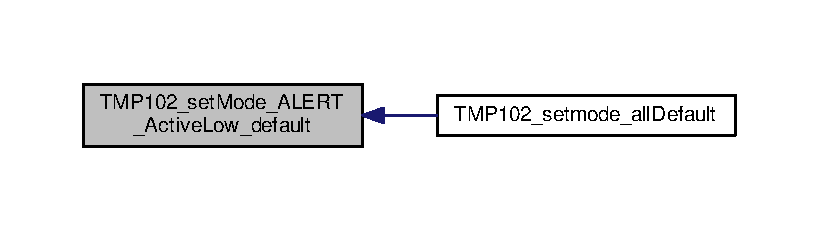
\includegraphics[width=350pt]{tmp102__sensor_8h_a899854f020db34f588f89adffcdc8433_icgraph}
\end{center}
\end{figure}


\index{tmp102\+\_\+sensor.\+h@{tmp102\+\_\+sensor.\+h}!T\+M\+P102\+\_\+setmode\+\_\+all\+Default@{T\+M\+P102\+\_\+setmode\+\_\+all\+Default}}
\index{T\+M\+P102\+\_\+setmode\+\_\+all\+Default@{T\+M\+P102\+\_\+setmode\+\_\+all\+Default}!tmp102\+\_\+sensor.\+h@{tmp102\+\_\+sensor.\+h}}
\subsubsection[{\texorpdfstring{T\+M\+P102\+\_\+setmode\+\_\+all\+Default()}{TMP102_setmode_allDefault()}}]{\setlength{\rightskip}{0pt plus 5cm}int T\+M\+P102\+\_\+setmode\+\_\+all\+Default (
\begin{DoxyParamCaption}
{}
\end{DoxyParamCaption}
)}\hypertarget{tmp102__sensor_8h_a4725fb3e4cf18de4220d6067a7dc5dd4}{}\label{tmp102__sensor_8h_a4725fb3e4cf18de4220d6067a7dc5dd4}


Brings back to default. 

\begin{DoxyReturn}{Returns}
int 
\end{DoxyReturn}

\begin{DoxyCode}
24 \{
25     \textcolor{keywordtype}{int} ret = \hyperlink{tmp102__sensor_8h_a6d24a33a5e009441edb99bd1a727afec}{TMP102\_setMode\_CR\_4HZ\_default}();
26     \textcolor{keywordflow}{if}(ret) \textcolor{keywordflow}{return} ret;
27     ret = \hyperlink{tmp102__sensor_8h_a4309a30e9d006753c2cdd6f6c9af2650}{TMP102\_setMode\_SD\_Continuous\_default}();
28     \textcolor{keywordflow}{if}(ret) \textcolor{keywordflow}{return} ret;
29     ret = \hyperlink{tmp102__sensor_8h_a899854f020db34f588f89adffcdc8433}{TMP102\_setMode\_ALERT\_ActiveLow\_default}();
30     \textcolor{keywordflow}{if}(ret) \textcolor{keywordflow}{return} ret;
31     ret = \hyperlink{tmp102__sensor_8h_a81c75dba63b6c0727ab602ea631b3a22}{TMP102\_setMode\_TM\_ComparatorMode\_default}();
32     \textcolor{keywordflow}{if}(ret) \textcolor{keywordflow}{return} ret;
33     ret = \hyperlink{tmp102__sensor_8h_aa96f470639b851a96f524ae6524dd266}{TMP102\_setMode\_EM\_NormalMode\_default}();
34     \textcolor{keywordflow}{return} ret;
35 \}
\end{DoxyCode}
\index{tmp102\+\_\+sensor.\+h@{tmp102\+\_\+sensor.\+h}!T\+M\+P102\+\_\+set\+Mode\+\_\+\+C\+R\+\_\+1\+HZ@{T\+M\+P102\+\_\+set\+Mode\+\_\+\+C\+R\+\_\+1\+HZ}}
\index{T\+M\+P102\+\_\+set\+Mode\+\_\+\+C\+R\+\_\+1\+HZ@{T\+M\+P102\+\_\+set\+Mode\+\_\+\+C\+R\+\_\+1\+HZ}!tmp102\+\_\+sensor.\+h@{tmp102\+\_\+sensor.\+h}}
\subsubsection[{\texorpdfstring{T\+M\+P102\+\_\+set\+Mode\+\_\+\+C\+R\+\_\+1\+H\+Z()}{TMP102_setMode_CR_1HZ()}}]{\setlength{\rightskip}{0pt plus 5cm}int T\+M\+P102\+\_\+set\+Mode\+\_\+\+C\+R\+\_\+1\+HZ (
\begin{DoxyParamCaption}
{}
\end{DoxyParamCaption}
)}\hypertarget{tmp102__sensor_8h_a110d2f8672865d85670f2681e5dc9aed}{}\label{tmp102__sensor_8h_a110d2f8672865d85670f2681e5dc9aed}
\begin{DoxyReturn}{Returns}
int 
\end{DoxyReturn}

\begin{DoxyCode}
189 \{
190     uint16\_t config\_data = 0;
191 
192      \textcolor{comment}{/* Reading the already configured values in the sensor */}
193     \textcolor{keywordtype}{int} ret = \hyperlink{my__i2c_8c_ab25650a9cf74e65561b1fced3555f36c}{I2Cmaster\_read\_bytes}(TMP102\_SLAVE\_ADDR, TMP102\_REG\_CONFIGURATION,(uint8\_t
      *)&config\_data, \textcolor{keyword}{sizeof}(config\_data));
194     \textcolor{keywordflow}{if}(ret == -1)
195         \textcolor{keywordflow}{return} ret;
196 
197     config\_data &= ~((uint16\_t)TMP102\_CONFIG\_CR(3));
198     config\_data |= ((uint16\_t)TMP102\_CONFIG\_CR(1)); 
199 
200     ret = \hyperlink{my__i2c_8c_a19c6244da5ea2d4e65a25001582498c8}{I2Cmaster\_write\_word}(TMP102\_SLAVE\_ADDR, TMP102\_REG\_CONFIGURATION, config\_data
      , 0);
201 
202     \textcolor{keywordflow}{return} ret;
203 
204 \}
\end{DoxyCode}
\index{tmp102\+\_\+sensor.\+h@{tmp102\+\_\+sensor.\+h}!T\+M\+P102\+\_\+set\+Mode\+\_\+\+C\+R\+\_\+250m\+HZ@{T\+M\+P102\+\_\+set\+Mode\+\_\+\+C\+R\+\_\+250m\+HZ}}
\index{T\+M\+P102\+\_\+set\+Mode\+\_\+\+C\+R\+\_\+250m\+HZ@{T\+M\+P102\+\_\+set\+Mode\+\_\+\+C\+R\+\_\+250m\+HZ}!tmp102\+\_\+sensor.\+h@{tmp102\+\_\+sensor.\+h}}
\subsubsection[{\texorpdfstring{T\+M\+P102\+\_\+set\+Mode\+\_\+\+C\+R\+\_\+250m\+H\+Z()}{TMP102_setMode_CR_250mHZ()}}]{\setlength{\rightskip}{0pt plus 5cm}int T\+M\+P102\+\_\+set\+Mode\+\_\+\+C\+R\+\_\+250m\+HZ (
\begin{DoxyParamCaption}
{}
\end{DoxyParamCaption}
)}\hypertarget{tmp102__sensor_8h_a3f6277d742af4a10dcec568e84ad1d5d}{}\label{tmp102__sensor_8h_a3f6277d742af4a10dcec568e84ad1d5d}
\begin{DoxyReturn}{Returns}
int 
\end{DoxyReturn}

\begin{DoxyCode}
173 \{
174     uint16\_t config\_data = 0;
175 
176      \textcolor{comment}{/* Reading the already configured values in the sensor */}
177     \textcolor{keywordtype}{int} ret = \hyperlink{my__i2c_8c_ab25650a9cf74e65561b1fced3555f36c}{I2Cmaster\_read\_bytes}(TMP102\_SLAVE\_ADDR, TMP102\_REG\_CONFIGURATION,(uint8\_t
      *)&config\_data, \textcolor{keyword}{sizeof}(config\_data));
178     \textcolor{keywordflow}{if}(ret == -1)
179         \textcolor{keywordflow}{return} ret;
180 
181     config\_data &= ~((uint16\_t)TMP102\_CONFIG\_CR(3)); 
182 
183     ret = \hyperlink{my__i2c_8c_a19c6244da5ea2d4e65a25001582498c8}{I2Cmaster\_write\_word}(TMP102\_SLAVE\_ADDR, TMP102\_REG\_CONFIGURATION, config\_data
      , 0);
184 
185     \textcolor{keywordflow}{return} ret;
186 
187 \}
\end{DoxyCode}
\index{tmp102\+\_\+sensor.\+h@{tmp102\+\_\+sensor.\+h}!T\+M\+P102\+\_\+set\+Mode\+\_\+\+C\+R\+\_\+4\+H\+Z\+\_\+default@{T\+M\+P102\+\_\+set\+Mode\+\_\+\+C\+R\+\_\+4\+H\+Z\+\_\+default}}
\index{T\+M\+P102\+\_\+set\+Mode\+\_\+\+C\+R\+\_\+4\+H\+Z\+\_\+default@{T\+M\+P102\+\_\+set\+Mode\+\_\+\+C\+R\+\_\+4\+H\+Z\+\_\+default}!tmp102\+\_\+sensor.\+h@{tmp102\+\_\+sensor.\+h}}
\subsubsection[{\texorpdfstring{T\+M\+P102\+\_\+set\+Mode\+\_\+\+C\+R\+\_\+4\+H\+Z\+\_\+default()}{TMP102_setMode_CR_4HZ_default()}}]{\setlength{\rightskip}{0pt plus 5cm}int T\+M\+P102\+\_\+set\+Mode\+\_\+\+C\+R\+\_\+4\+H\+Z\+\_\+default (
\begin{DoxyParamCaption}
{}
\end{DoxyParamCaption}
)}\hypertarget{tmp102__sensor_8h_a6d24a33a5e009441edb99bd1a727afec}{}\label{tmp102__sensor_8h_a6d24a33a5e009441edb99bd1a727afec}
\begin{DoxyReturn}{Returns}
int 
\end{DoxyReturn}

\begin{DoxyCode}
206 \{
207     uint16\_t config\_data = 0;
208 
209      \textcolor{comment}{/* Reading the already configured values in the sensor */}
210     \textcolor{keywordtype}{int} ret = \hyperlink{my__i2c_8c_ab25650a9cf74e65561b1fced3555f36c}{I2Cmaster\_read\_bytes}(TMP102\_SLAVE\_ADDR, TMP102\_REG\_CONFIGURATION,(uint8\_t
      *)&config\_data, \textcolor{keyword}{sizeof}(config\_data));
211     \textcolor{keywordflow}{if}(ret == -1)
212         \textcolor{keywordflow}{return} ret;
213 
214     config\_data &= ~((uint16\_t)TMP102\_CONFIG\_CR(3));
215     config\_data |= ((uint16\_t)TMP102\_CONFIG\_CR(2)); 
216 
217     ret = \hyperlink{my__i2c_8c_a19c6244da5ea2d4e65a25001582498c8}{I2Cmaster\_write\_word}(TMP102\_SLAVE\_ADDR, TMP102\_REG\_CONFIGURATION, config\_data
      , 0);
218 
219     \textcolor{keywordflow}{return} ret;
220 
221 \}
\end{DoxyCode}


Here is the caller graph for this function\+:\nopagebreak
\begin{figure}[H]
\begin{center}
\leavevmode
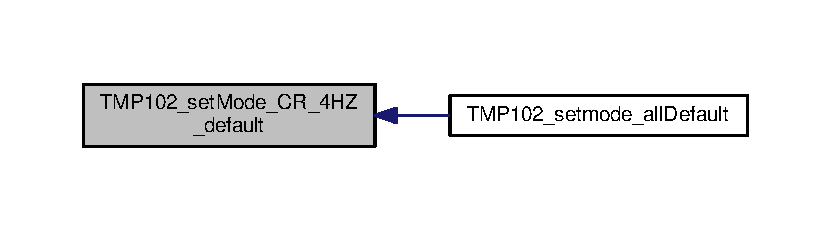
\includegraphics[width=350pt]{tmp102__sensor_8h_a6d24a33a5e009441edb99bd1a727afec_icgraph}
\end{center}
\end{figure}


\index{tmp102\+\_\+sensor.\+h@{tmp102\+\_\+sensor.\+h}!T\+M\+P102\+\_\+set\+Mode\+\_\+\+C\+R\+\_\+8\+HZ@{T\+M\+P102\+\_\+set\+Mode\+\_\+\+C\+R\+\_\+8\+HZ}}
\index{T\+M\+P102\+\_\+set\+Mode\+\_\+\+C\+R\+\_\+8\+HZ@{T\+M\+P102\+\_\+set\+Mode\+\_\+\+C\+R\+\_\+8\+HZ}!tmp102\+\_\+sensor.\+h@{tmp102\+\_\+sensor.\+h}}
\subsubsection[{\texorpdfstring{T\+M\+P102\+\_\+set\+Mode\+\_\+\+C\+R\+\_\+8\+H\+Z()}{TMP102_setMode_CR_8HZ()}}]{\setlength{\rightskip}{0pt plus 5cm}int T\+M\+P102\+\_\+set\+Mode\+\_\+\+C\+R\+\_\+8\+HZ (
\begin{DoxyParamCaption}
{}
\end{DoxyParamCaption}
)}\hypertarget{tmp102__sensor_8h_a031c7291b177515876ebb29d24dc97b4}{}\label{tmp102__sensor_8h_a031c7291b177515876ebb29d24dc97b4}
\begin{DoxyReturn}{Returns}
int 
\end{DoxyReturn}

\begin{DoxyCode}
224 \{
225     uint16\_t config\_data = 0;
226 
227      \textcolor{comment}{/* Reading the already configured values in the sensor */}
228     \textcolor{keywordtype}{int} ret = \hyperlink{my__i2c_8c_ab25650a9cf74e65561b1fced3555f36c}{I2Cmaster\_read\_bytes}(TMP102\_SLAVE\_ADDR, TMP102\_REG\_CONFIGURATION,(uint8\_t
      *)&config\_data, \textcolor{keyword}{sizeof}(config\_data));
229     \textcolor{keywordflow}{if}(ret == -1)
230         \textcolor{keywordflow}{return} ret;
231 
232     config\_data |= ((uint16\_t)TMP102\_CONFIG\_CR(3)); 
233 
234     ret = \hyperlink{my__i2c_8c_a19c6244da5ea2d4e65a25001582498c8}{I2Cmaster\_write\_word}(TMP102\_SLAVE\_ADDR, TMP102\_REG\_CONFIGURATION, config\_data
      , 0);
235 
236     \textcolor{keywordflow}{return} ret;
237 
238 \}
\end{DoxyCode}
\index{tmp102\+\_\+sensor.\+h@{tmp102\+\_\+sensor.\+h}!T\+M\+P102\+\_\+set\+Mode\+\_\+\+E\+M\+\_\+\+Extended\+Mode@{T\+M\+P102\+\_\+set\+Mode\+\_\+\+E\+M\+\_\+\+Extended\+Mode}}
\index{T\+M\+P102\+\_\+set\+Mode\+\_\+\+E\+M\+\_\+\+Extended\+Mode@{T\+M\+P102\+\_\+set\+Mode\+\_\+\+E\+M\+\_\+\+Extended\+Mode}!tmp102\+\_\+sensor.\+h@{tmp102\+\_\+sensor.\+h}}
\subsubsection[{\texorpdfstring{T\+M\+P102\+\_\+set\+Mode\+\_\+\+E\+M\+\_\+\+Extended\+Mode()}{TMP102_setMode_EM_ExtendedMode()}}]{\setlength{\rightskip}{0pt plus 5cm}int T\+M\+P102\+\_\+set\+Mode\+\_\+\+E\+M\+\_\+\+Extended\+Mode (
\begin{DoxyParamCaption}
{}
\end{DoxyParamCaption}
)}\hypertarget{tmp102__sensor_8h_a2df18183afad1339903fe59997aaf9a2}{}\label{tmp102__sensor_8h_a2df18183afad1339903fe59997aaf9a2}
\begin{DoxyReturn}{Returns}
int 
\end{DoxyReturn}

\begin{DoxyCode}
157 \{
158     uint16\_t config\_data = 0;
159 
160      \textcolor{comment}{/* Reading the already configured values in the sensor */}
161     \textcolor{keywordtype}{int} ret = \hyperlink{my__i2c_8c_ab25650a9cf74e65561b1fced3555f36c}{I2Cmaster\_read\_bytes}(TMP102\_SLAVE\_ADDR, TMP102\_REG\_CONFIGURATION,(uint8\_t
      *)&config\_data, \textcolor{keyword}{sizeof}(config\_data));
162     \textcolor{keywordflow}{if}(ret == -1)
163         \textcolor{keywordflow}{return} ret;
164 
165     config\_data |= (uint16\_t)TMP102\_CONFIG\_EM; 
166 
167     ret = \hyperlink{my__i2c_8c_a19c6244da5ea2d4e65a25001582498c8}{I2Cmaster\_write\_word}(TMP102\_SLAVE\_ADDR, TMP102\_REG\_CONFIGURATION, config\_data
      , 0);
168 
169     \textcolor{keywordflow}{return} ret;
170 
171 \}
\end{DoxyCode}
\index{tmp102\+\_\+sensor.\+h@{tmp102\+\_\+sensor.\+h}!T\+M\+P102\+\_\+set\+Mode\+\_\+\+E\+M\+\_\+\+Normal\+Mode\+\_\+default@{T\+M\+P102\+\_\+set\+Mode\+\_\+\+E\+M\+\_\+\+Normal\+Mode\+\_\+default}}
\index{T\+M\+P102\+\_\+set\+Mode\+\_\+\+E\+M\+\_\+\+Normal\+Mode\+\_\+default@{T\+M\+P102\+\_\+set\+Mode\+\_\+\+E\+M\+\_\+\+Normal\+Mode\+\_\+default}!tmp102\+\_\+sensor.\+h@{tmp102\+\_\+sensor.\+h}}
\subsubsection[{\texorpdfstring{T\+M\+P102\+\_\+set\+Mode\+\_\+\+E\+M\+\_\+\+Normal\+Mode\+\_\+default()}{TMP102_setMode_EM_NormalMode_default()}}]{\setlength{\rightskip}{0pt plus 5cm}int T\+M\+P102\+\_\+set\+Mode\+\_\+\+E\+M\+\_\+\+Normal\+Mode\+\_\+default (
\begin{DoxyParamCaption}
{}
\end{DoxyParamCaption}
)}\hypertarget{tmp102__sensor_8h_aa96f470639b851a96f524ae6524dd266}{}\label{tmp102__sensor_8h_aa96f470639b851a96f524ae6524dd266}
\begin{DoxyReturn}{Returns}
int 
\end{DoxyReturn}

\begin{DoxyCode}
140 \{
141     uint16\_t config\_data = 0;
142 
143      \textcolor{comment}{/* Reading the already configured values in the sensor */}
144     \textcolor{keywordtype}{int} ret = \hyperlink{my__i2c_8c_ab25650a9cf74e65561b1fced3555f36c}{I2Cmaster\_read\_bytes}(TMP102\_SLAVE\_ADDR, TMP102\_REG\_CONFIGURATION,(uint8\_t
      *)&config\_data, \textcolor{keyword}{sizeof}(config\_data));
145     \textcolor{keywordflow}{if}(ret == -1)
146         \textcolor{keywordflow}{return} ret;
147 
148     config\_data &= ~((uint16\_t)TMP102\_CONFIG\_EM); 
149 
150     ret = \hyperlink{my__i2c_8c_a19c6244da5ea2d4e65a25001582498c8}{I2Cmaster\_write\_word}(TMP102\_SLAVE\_ADDR, TMP102\_REG\_CONFIGURATION, config\_data
      , 0);
151 
152     \textcolor{keywordflow}{return} ret;
153 
154 
155 \}
\end{DoxyCode}


Here is the caller graph for this function\+:\nopagebreak
\begin{figure}[H]
\begin{center}
\leavevmode
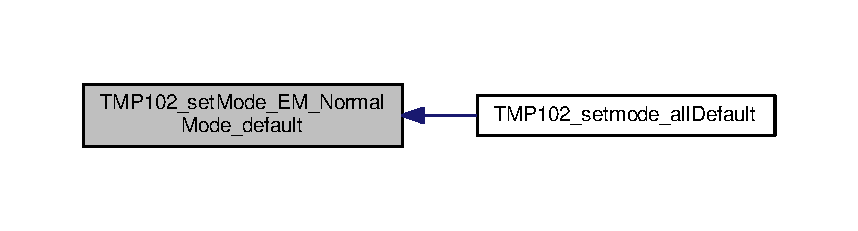
\includegraphics[width=350pt]{tmp102__sensor_8h_aa96f470639b851a96f524ae6524dd266_icgraph}
\end{center}
\end{figure}


\index{tmp102\+\_\+sensor.\+h@{tmp102\+\_\+sensor.\+h}!T\+M\+P102\+\_\+set\+Mode\+\_\+\+S\+D\+\_\+\+Continuous\+\_\+default@{T\+M\+P102\+\_\+set\+Mode\+\_\+\+S\+D\+\_\+\+Continuous\+\_\+default}}
\index{T\+M\+P102\+\_\+set\+Mode\+\_\+\+S\+D\+\_\+\+Continuous\+\_\+default@{T\+M\+P102\+\_\+set\+Mode\+\_\+\+S\+D\+\_\+\+Continuous\+\_\+default}!tmp102\+\_\+sensor.\+h@{tmp102\+\_\+sensor.\+h}}
\subsubsection[{\texorpdfstring{T\+M\+P102\+\_\+set\+Mode\+\_\+\+S\+D\+\_\+\+Continuous\+\_\+default()}{TMP102_setMode_SD_Continuous_default()}}]{\setlength{\rightskip}{0pt plus 5cm}int T\+M\+P102\+\_\+set\+Mode\+\_\+\+S\+D\+\_\+\+Continuous\+\_\+default (
\begin{DoxyParamCaption}
{}
\end{DoxyParamCaption}
)}\hypertarget{tmp102__sensor_8h_a4309a30e9d006753c2cdd6f6c9af2650}{}\label{tmp102__sensor_8h_a4309a30e9d006753c2cdd6f6c9af2650}
\begin{DoxyReturn}{Returns}
int 
\end{DoxyReturn}

\begin{DoxyCode}
60 \{
61     uint16\_t config\_data = 0;
62 
63      \textcolor{comment}{/* Reading the already configured values in the sensor */}
64     \textcolor{keywordtype}{int} ret = \hyperlink{my__i2c_8c_ab25650a9cf74e65561b1fced3555f36c}{I2Cmaster\_read\_bytes}(TMP102\_SLAVE\_ADDR, TMP102\_REG\_CONFIGURATION,(uint8\_t
      *)&config\_data, \textcolor{keyword}{sizeof}(config\_data));
65     \textcolor{keywordflow}{if}(ret == -1)
66         \textcolor{keywordflow}{return} ret;
67 
68     config\_data &= ~((uint16\_t)TMP102\_CONFIG\_SD); 
69 
70     ret = \hyperlink{my__i2c_8c_a19c6244da5ea2d4e65a25001582498c8}{I2Cmaster\_write\_word}(TMP102\_SLAVE\_ADDR, TMP102\_REG\_CONFIGURATION, config\_data
      , 0);
71 
72     \textcolor{keywordflow}{return} ret;
73 \}
\end{DoxyCode}


Here is the caller graph for this function\+:\nopagebreak
\begin{figure}[H]
\begin{center}
\leavevmode
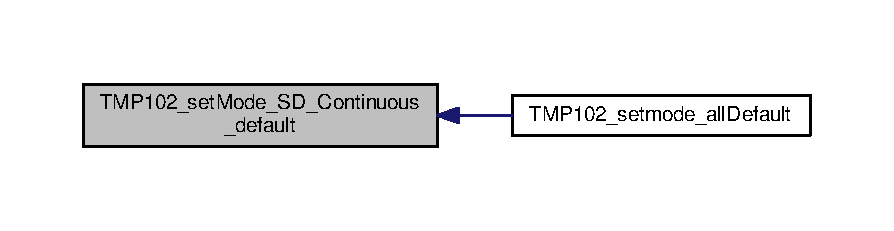
\includegraphics[width=350pt]{tmp102__sensor_8h_a4309a30e9d006753c2cdd6f6c9af2650_icgraph}
\end{center}
\end{figure}


\index{tmp102\+\_\+sensor.\+h@{tmp102\+\_\+sensor.\+h}!T\+M\+P102\+\_\+set\+Mode\+\_\+\+S\+D\+\_\+\+Power\+Saving@{T\+M\+P102\+\_\+set\+Mode\+\_\+\+S\+D\+\_\+\+Power\+Saving}}
\index{T\+M\+P102\+\_\+set\+Mode\+\_\+\+S\+D\+\_\+\+Power\+Saving@{T\+M\+P102\+\_\+set\+Mode\+\_\+\+S\+D\+\_\+\+Power\+Saving}!tmp102\+\_\+sensor.\+h@{tmp102\+\_\+sensor.\+h}}
\subsubsection[{\texorpdfstring{T\+M\+P102\+\_\+set\+Mode\+\_\+\+S\+D\+\_\+\+Power\+Saving()}{TMP102_setMode_SD_PowerSaving()}}]{\setlength{\rightskip}{0pt plus 5cm}int T\+M\+P102\+\_\+set\+Mode\+\_\+\+S\+D\+\_\+\+Power\+Saving (
\begin{DoxyParamCaption}
{}
\end{DoxyParamCaption}
)}\hypertarget{tmp102__sensor_8h_a7d4d57387ef6a5db5bfc8d14a94d9ee4}{}\label{tmp102__sensor_8h_a7d4d57387ef6a5db5bfc8d14a94d9ee4}
\begin{DoxyReturn}{Returns}
int 
\end{DoxyReturn}

\begin{DoxyCode}
44 \{
45     uint16\_t config\_data = 0;
46 
47      \textcolor{comment}{/* Reading the already configured values in the sensor */}
48     \textcolor{keywordtype}{int} ret = \hyperlink{my__i2c_8c_ab25650a9cf74e65561b1fced3555f36c}{I2Cmaster\_read\_bytes}(TMP102\_SLAVE\_ADDR, TMP102\_REG\_CONFIGURATION,(uint8\_t
      *)&config\_data, \textcolor{keyword}{sizeof}(config\_data));
49     \textcolor{keywordflow}{if}(ret == -1)
50         \textcolor{keywordflow}{return} ret;
51 
52     config\_data |= (uint16\_t)TMP102\_CONFIG\_SD; 
53 
54     ret = \hyperlink{my__i2c_8c_a19c6244da5ea2d4e65a25001582498c8}{I2Cmaster\_write\_word}(TMP102\_SLAVE\_ADDR, TMP102\_REG\_CONFIGURATION, config\_data
      , 0);
55 
56     \textcolor{keywordflow}{return} ret;
57 
58 \}
\end{DoxyCode}
\index{tmp102\+\_\+sensor.\+h@{tmp102\+\_\+sensor.\+h}!T\+M\+P102\+\_\+set\+Mode\+\_\+\+T\+M\+\_\+\+Comparator\+Mode\+\_\+default@{T\+M\+P102\+\_\+set\+Mode\+\_\+\+T\+M\+\_\+\+Comparator\+Mode\+\_\+default}}
\index{T\+M\+P102\+\_\+set\+Mode\+\_\+\+T\+M\+\_\+\+Comparator\+Mode\+\_\+default@{T\+M\+P102\+\_\+set\+Mode\+\_\+\+T\+M\+\_\+\+Comparator\+Mode\+\_\+default}!tmp102\+\_\+sensor.\+h@{tmp102\+\_\+sensor.\+h}}
\subsubsection[{\texorpdfstring{T\+M\+P102\+\_\+set\+Mode\+\_\+\+T\+M\+\_\+\+Comparator\+Mode\+\_\+default()}{TMP102_setMode_TM_ComparatorMode_default()}}]{\setlength{\rightskip}{0pt plus 5cm}int T\+M\+P102\+\_\+set\+Mode\+\_\+\+T\+M\+\_\+\+Comparator\+Mode\+\_\+default (
\begin{DoxyParamCaption}
{}
\end{DoxyParamCaption}
)}\hypertarget{tmp102__sensor_8h_a81c75dba63b6c0727ab602ea631b3a22}{}\label{tmp102__sensor_8h_a81c75dba63b6c0727ab602ea631b3a22}
\begin{DoxyReturn}{Returns}
int 
\end{DoxyReturn}

\begin{DoxyCode}
76 \{
77     uint16\_t config\_data = 0;
78 
79      \textcolor{comment}{/* Reading the already configured values in the sensor */}
80     \textcolor{keywordtype}{int} ret = \hyperlink{my__i2c_8c_ab25650a9cf74e65561b1fced3555f36c}{I2Cmaster\_read\_bytes}(TMP102\_SLAVE\_ADDR, TMP102\_REG\_CONFIGURATION,(uint8\_t
      *)&config\_data, \textcolor{keyword}{sizeof}(config\_data));
81     \textcolor{keywordflow}{if}(ret == -1)
82         \textcolor{keywordflow}{return} ret;
83 
84     config\_data &= ~((uint16\_t)TMP102\_CONFIG\_TM); 
85 
86     ret = \hyperlink{my__i2c_8c_a19c6244da5ea2d4e65a25001582498c8}{I2Cmaster\_write\_word}(TMP102\_SLAVE\_ADDR, TMP102\_REG\_CONFIGURATION, config\_data
      , 0);
87 
88     \textcolor{keywordflow}{return} ret;
89 
90 \}
\end{DoxyCode}


Here is the caller graph for this function\+:\nopagebreak
\begin{figure}[H]
\begin{center}
\leavevmode
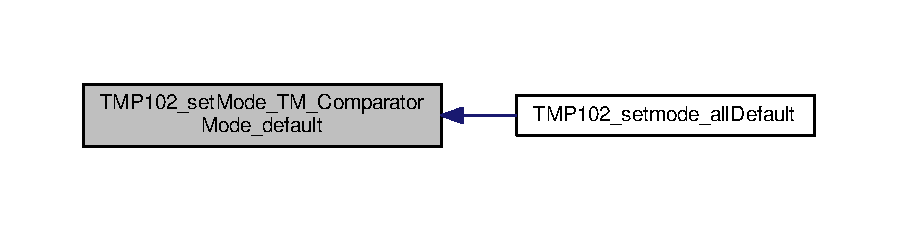
\includegraphics[width=350pt]{tmp102__sensor_8h_a81c75dba63b6c0727ab602ea631b3a22_icgraph}
\end{center}
\end{figure}


\index{tmp102\+\_\+sensor.\+h@{tmp102\+\_\+sensor.\+h}!T\+M\+P102\+\_\+set\+Mode\+\_\+\+T\+M\+\_\+\+Interrupt\+Mode@{T\+M\+P102\+\_\+set\+Mode\+\_\+\+T\+M\+\_\+\+Interrupt\+Mode}}
\index{T\+M\+P102\+\_\+set\+Mode\+\_\+\+T\+M\+\_\+\+Interrupt\+Mode@{T\+M\+P102\+\_\+set\+Mode\+\_\+\+T\+M\+\_\+\+Interrupt\+Mode}!tmp102\+\_\+sensor.\+h@{tmp102\+\_\+sensor.\+h}}
\subsubsection[{\texorpdfstring{T\+M\+P102\+\_\+set\+Mode\+\_\+\+T\+M\+\_\+\+Interrupt\+Mode()}{TMP102_setMode_TM_InterruptMode()}}]{\setlength{\rightskip}{0pt plus 5cm}int T\+M\+P102\+\_\+set\+Mode\+\_\+\+T\+M\+\_\+\+Interrupt\+Mode (
\begin{DoxyParamCaption}
{}
\end{DoxyParamCaption}
)}\hypertarget{tmp102__sensor_8h_a4386703b35277dc71be5cd9b57d0f3ce}{}\label{tmp102__sensor_8h_a4386703b35277dc71be5cd9b57d0f3ce}
\begin{DoxyReturn}{Returns}
int 
\end{DoxyReturn}

\begin{DoxyCode}
92 \{
93     uint16\_t config\_data = 0;
94 
95      \textcolor{comment}{/* Reading the already configured values in the sensor */}
96     \textcolor{keywordtype}{int} ret = \hyperlink{my__i2c_8c_ab25650a9cf74e65561b1fced3555f36c}{I2Cmaster\_read\_bytes}(TMP102\_SLAVE\_ADDR, TMP102\_REG\_CONFIGURATION,(uint8\_t
      *)&config\_data, \textcolor{keyword}{sizeof}(config\_data));
97     \textcolor{keywordflow}{if}(ret == -1)
98         \textcolor{keywordflow}{return} ret;
99 
100     config\_data |= (uint16\_t)TMP102\_CONFIG\_TM; 
101 
102     ret = \hyperlink{my__i2c_8c_a19c6244da5ea2d4e65a25001582498c8}{I2Cmaster\_write\_word}(TMP102\_SLAVE\_ADDR, TMP102\_REG\_CONFIGURATION, config\_data
      , 0);
103 
104     \textcolor{keywordflow}{return} ret;
105 
106 \}
\end{DoxyCode}
\index{tmp102\+\_\+sensor.\+h@{tmp102\+\_\+sensor.\+h}!T\+M\+P102\+\_\+write\+\_\+\+Thigh@{T\+M\+P102\+\_\+write\+\_\+\+Thigh}}
\index{T\+M\+P102\+\_\+write\+\_\+\+Thigh@{T\+M\+P102\+\_\+write\+\_\+\+Thigh}!tmp102\+\_\+sensor.\+h@{tmp102\+\_\+sensor.\+h}}
\subsubsection[{\texorpdfstring{T\+M\+P102\+\_\+write\+\_\+\+Thigh(float thigh\+\_\+\+C)}{TMP102_write_Thigh(float thigh_C)}}]{\setlength{\rightskip}{0pt plus 5cm}int T\+M\+P102\+\_\+write\+\_\+\+Thigh (
\begin{DoxyParamCaption}
\item[{float}]{thigh\+\_\+C}
\end{DoxyParamCaption}
)}\hypertarget{tmp102__sensor_8h_a32a4b8bbc5611a7ca967cdaaeb732ae1}{}\label{tmp102__sensor_8h_a32a4b8bbc5611a7ca967cdaaeb732ae1}

\begin{DoxyParams}{Parameters}
{\em thigh\+\_\+C} & \\
\hline
\end{DoxyParams}
\begin{DoxyReturn}{Returns}
int 
\end{DoxyReturn}

\begin{DoxyCode}
291 \{
292 
293     \textcolor{keywordflow}{if}(thigh\_C < -56.0f || thigh\_C > 151.0f)
294         thigh\_C = 80.0f;
295     
296     thigh\_C /= 0.0625;
297     uint16\_t th;
298 
299     \textcolor{keywordflow}{if}(thigh\_C > 0)
300     \{
301         th = ((uint16\_t)thigh\_C << 4);
302         th &= 0x7FFF;
303     \}
304     \textcolor{keywordflow}{else}
305     \{
306         thigh\_C = -1 * thigh\_C;
307         th = (uint16\_t)thigh\_C;
308         th = ~(th) + 1;
309         th = th << 4; 
310     \}  
311     
312     \textcolor{keywordtype}{int} ret = \hyperlink{my__i2c_8c_a19c6244da5ea2d4e65a25001582498c8}{I2Cmaster\_write\_word}(TMP102\_SLAVE\_ADDR, TMP102\_REG\_TLOW, th, 0);
313     \textcolor{keywordflow}{if}(ret == -1)
314         \textcolor{keywordflow}{return} ret;
315 
316 \textcolor{preprocessor}{    #ifdef TEST\_I2C}
317     uint16\_t ret =0;
318     ret = \hyperlink{my__i2c_8c_ab25650a9cf74e65561b1fced3555f36c}{I2Cmaster\_read\_bytes}(TMP102\_SLAVE\_ADDR, TMP102\_REG\_TLOW,(uint8\_t*)&ret, \textcolor{keyword}{
      sizeof}(ret));
319     \textcolor{keywordflow}{if}(ret == -1)
320         \textcolor{keywordflow}{return} ret;
321     
322     assert(ret == th);
323     assert\_true(ret == th);
324 \textcolor{preprocessor}{    #endif}
325 
326 
327 \}
\end{DoxyCode}
\index{tmp102\+\_\+sensor.\+h@{tmp102\+\_\+sensor.\+h}!T\+M\+P102\+\_\+write\+\_\+\+Tlow@{T\+M\+P102\+\_\+write\+\_\+\+Tlow}}
\index{T\+M\+P102\+\_\+write\+\_\+\+Tlow@{T\+M\+P102\+\_\+write\+\_\+\+Tlow}!tmp102\+\_\+sensor.\+h@{tmp102\+\_\+sensor.\+h}}
\subsubsection[{\texorpdfstring{T\+M\+P102\+\_\+write\+\_\+\+Tlow(float tlow\+\_\+\+C)}{TMP102_write_Tlow(float tlow_C)}}]{\setlength{\rightskip}{0pt plus 5cm}int T\+M\+P102\+\_\+write\+\_\+\+Tlow (
\begin{DoxyParamCaption}
\item[{float}]{tlow\+\_\+C}
\end{DoxyParamCaption}
)}\hypertarget{tmp102__sensor_8h_a6296f70167b1f662c7f9b56b15fe037c}{}\label{tmp102__sensor_8h_a6296f70167b1f662c7f9b56b15fe037c}

\begin{DoxyParams}{Parameters}
{\em tlow\+\_\+C} & \\
\hline
\end{DoxyParams}
\begin{DoxyReturn}{Returns}
int 
\end{DoxyReturn}

\begin{DoxyCode}
254 \{
255     \textcolor{keywordflow}{if}(tlow\_C < -56.0f || tlow\_C > 151.0f)
256         tlow\_C = 75.0f;
257     
258     tlow\_C /= 0.0625;
259     uint16\_t tl;
260 
261     \textcolor{keywordflow}{if}(tlow\_C > 0)
262     \{
263         tl = ((uint16\_t)tlow\_C << 4);
264         tl &= 0x7FFF;
265     \}
266     \textcolor{keywordflow}{else}
267     \{
268         tlow\_C = -1 * tlow\_C;
269         tl = (uint16\_t)tlow\_C;
270         tl = ~(tl) + 1;
271         tl = tl << 4; 
272     \}  
273     
274     \textcolor{keywordtype}{int} ret = \hyperlink{my__i2c_8c_a19c6244da5ea2d4e65a25001582498c8}{I2Cmaster\_write\_word}(TMP102\_SLAVE\_ADDR, TMP102\_REG\_TLOW, tl, 0);
275     \textcolor{keywordflow}{if}(ret == -1)
276         \textcolor{keywordflow}{return} ret;
277 
278 \textcolor{preprocessor}{    #ifdef TEST\_I2C}
279     uint16\_t retTlow =0;
280     ret = \hyperlink{my__i2c_8c_ab25650a9cf74e65561b1fced3555f36c}{I2Cmaster\_read\_bytes}(TMP102\_SLAVE\_ADDR, TMP102\_REG\_TLOW,(uint8\_t*)&retTlow, \textcolor{keyword}{
      sizeof}(retTlow));
281     \textcolor{keywordflow}{if}(ret == -1)
282         \textcolor{keywordflow}{return} ret;
283     
284     assert(retTlow == tl);
285     assert\_int\_equal(retTlow,tl);
286 \textcolor{preprocessor}{    #endif}
287          
288 \}
\end{DoxyCode}


\subsection{Variable Documentation}
\index{tmp102\+\_\+sensor.\+h@{tmp102\+\_\+sensor.\+h}!T\+M\+P102\+\_\+\+C\+O\+N\+F\+I\+G\+\_\+\+D\+E\+F\+A\+U\+LT@{T\+M\+P102\+\_\+\+C\+O\+N\+F\+I\+G\+\_\+\+D\+E\+F\+A\+U\+LT}}
\index{T\+M\+P102\+\_\+\+C\+O\+N\+F\+I\+G\+\_\+\+D\+E\+F\+A\+U\+LT@{T\+M\+P102\+\_\+\+C\+O\+N\+F\+I\+G\+\_\+\+D\+E\+F\+A\+U\+LT}!tmp102\+\_\+sensor.\+h@{tmp102\+\_\+sensor.\+h}}
\subsubsection[{\texorpdfstring{T\+M\+P102\+\_\+\+C\+O\+N\+F\+I\+G\+\_\+\+D\+E\+F\+A\+U\+LT}{TMP102_CONFIG_DEFAULT}}]{\setlength{\rightskip}{0pt plus 5cm}const {\bf T\+M\+P102\+\_\+\+C\+O\+N\+F\+I\+G\+\_\+\+R\+E\+G\+\_\+\+S\+E\+T\+T\+I\+N\+G\+S\+\_\+T} T\+M\+P102\+\_\+\+C\+O\+N\+F\+I\+G\+\_\+\+D\+E\+F\+A\+U\+LT}\hypertarget{tmp102__sensor_8h_ae8c25eda33c17bf746db7b91fe54c85c}{}\label{tmp102__sensor_8h_ae8c25eda33c17bf746db7b91fe54c85c}

\begin{DoxyParams}{Parameters}
{\em temp} & \\
\hline
{\em unit} & \\
\hline
\end{DoxyParams}
\begin{DoxyReturn}{Returns}
int 
\end{DoxyReturn}

\hypertarget{common__helper_8h}{}\section{/home/gunj/repos/\+E\+C\+E\+N-\/5013/\+Project1/include/common/common\+\_\+helper.h File Reference}
\label{common__helper_8h}\index{/home/gunj/repos/\+E\+C\+E\+N-\/5013/\+Project1/include/common/common\+\_\+helper.\+h@{/home/gunj/repos/\+E\+C\+E\+N-\/5013/\+Project1/include/common/common\+\_\+helper.\+h}}
{\ttfamily \#include $<$mqueue.\+h$>$}\\*
{\ttfamily \#include $<$pthread.\+h$>$}\\*
{\ttfamily \#include \char`\"{}posix\+Timer.\+h\char`\"{}}\\*
Include dependency graph for common\+\_\+helper.\+h\+:\nopagebreak
\begin{figure}[H]
\begin{center}
\leavevmode
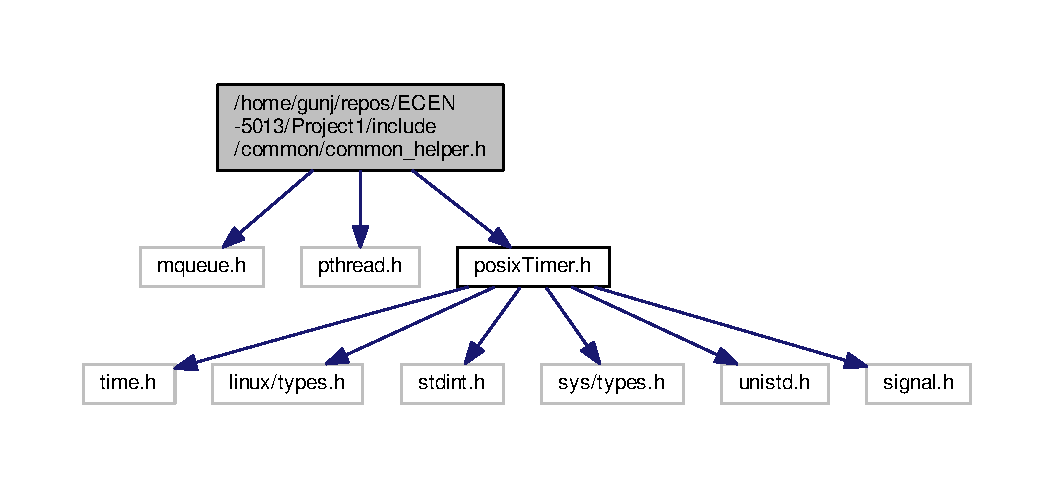
\includegraphics[width=350pt]{common__helper_8h__incl}
\end{center}
\end{figure}
This graph shows which files directly or indirectly include this file\+:\nopagebreak
\begin{figure}[H]
\begin{center}
\leavevmode
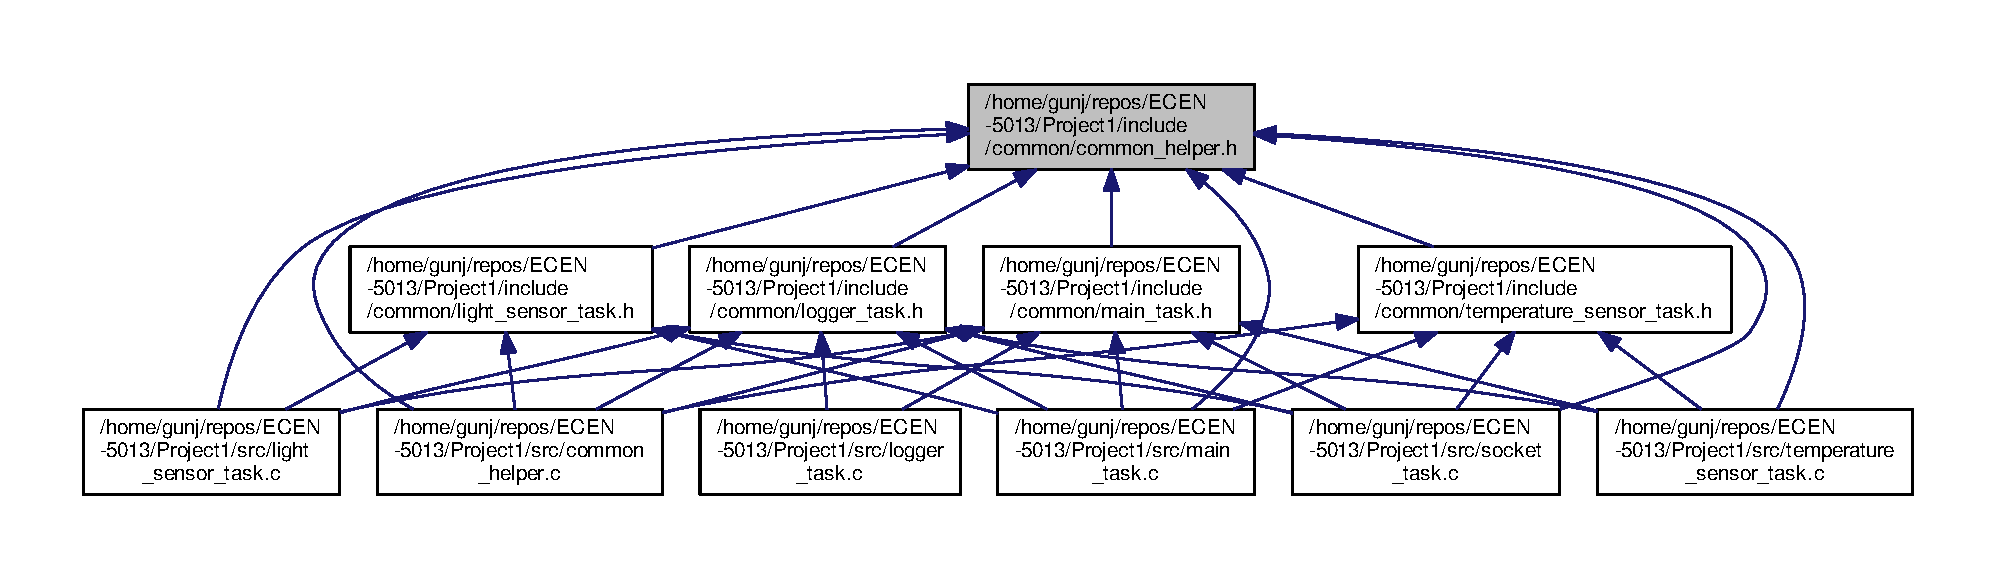
\includegraphics[width=350pt]{common__helper_8h__dep__incl}
\end{center}
\end{figure}
\subsection*{Macros}
\begin{DoxyCompactItemize}
\item 
\#define {\bfseries N\+U\+M\+\_\+\+C\+H\+I\+L\+D\+\_\+\+T\+H\+R\+E\+A\+DS}~4\hypertarget{common__helper_8h_aeb3dea598800d76fb6df4e66eb87eaf2}{}\label{common__helper_8h_aeb3dea598800d76fb6df4e66eb87eaf2}

\end{DoxyCompactItemize}
\subsection*{Enumerations}
\begin{DoxyCompactItemize}
\item 
enum {\bfseries T\+A\+S\+K\+\_\+\+I\+D\+E\+N\+T\+I\+F\+I\+E\+R\+\_\+T} \{ \\*
{\bfseries L\+O\+G\+G\+E\+R\+\_\+\+T\+A\+S\+K\+\_\+\+ID}, 
{\bfseries T\+E\+M\+P\+E\+R\+A\+T\+U\+R\+E\+\_\+\+T\+A\+S\+K\+\_\+\+ID}, 
{\bfseries S\+O\+C\+K\+E\+T\+\_\+\+T\+A\+S\+K\+\_\+\+ID}, 
{\bfseries L\+I\+G\+H\+T\+\_\+\+T\+A\+S\+K\+\_\+\+ID}, 
\\*
{\bfseries M\+A\+I\+N\+\_\+\+T\+A\+S\+K\+\_\+\+ID}
 \}\hypertarget{common__helper_8h_a8d5b3d16175933541aa53f183b77f2ae}{}\label{common__helper_8h_a8d5b3d16175933541aa53f183b77f2ae}

\end{DoxyCompactItemize}
\subsection*{Functions}
\begin{DoxyCompactItemize}
\item 
mqd\+\_\+t {\bfseries get\+\_\+queue\+\_\+handle} (T\+A\+S\+K\+\_\+\+I\+D\+E\+N\+T\+I\+F\+I\+E\+R\+\_\+T taskid)\hypertarget{common__helper_8h_ae2992ef59a491948e3b031929e7b130e}{}\label{common__helper_8h_ae2992ef59a491948e3b031929e7b130e}

\item 
int \hyperlink{common__helper_8h_a23124253b968391b9777fc3b8a0cc5ec}{register\+\_\+and\+\_\+start\+\_\+timer} (timer\+\_\+t $\ast$timer\+\_\+id, uint32\+\_\+t usec, uint8\+\_\+t oneshot, void($\ast$timer\+\_\+handler)(union sigval), void $\ast$handler\+Args)
\begin{DoxyCompactList}\small\item\em Registers a timer, addigns the handler and starts it. \end{DoxyCompactList}\end{DoxyCompactItemize}
\subsection*{Variables}
\begin{DoxyCompactItemize}
\item 
volatile int {\bfseries alive\+Status} \mbox{[}N\+U\+M\+\_\+\+C\+H\+I\+L\+D\+\_\+\+T\+H\+R\+E\+A\+DS\mbox{]}\hypertarget{common__helper_8h_af5d4df1bffe487c45323aa4f523d8f31}{}\label{common__helper_8h_af5d4df1bffe487c45323aa4f523d8f31}

\item 
pthread\+\_\+mutex\+\_\+t {\bfseries alive\+State\+\_\+lock}\hypertarget{common__helper_8h_a39d6b183fe81ea1b36bb46c0344c036b}{}\label{common__helper_8h_a39d6b183fe81ea1b36bb46c0344c036b}

\item 
pthread\+\_\+t {\bfseries pthread\+\_\+id} \mbox{[}N\+U\+M\+\_\+\+C\+H\+I\+L\+D\+\_\+\+T\+H\+R\+E\+A\+DS\mbox{]}\hypertarget{common__helper_8h_a6e37d77f5e9dbfd89885b25b3d82e5b3}{}\label{common__helper_8h_a6e37d77f5e9dbfd89885b25b3d82e5b3}

\item 
pthread\+\_\+barrier\+\_\+t {\bfseries tasks\+\_\+barrier}\hypertarget{common__helper_8h_a69daefcb62e8c68de7d59303754d7a21}{}\label{common__helper_8h_a69daefcb62e8c68de7d59303754d7a21}

\item 
const char $\ast$const {\bfseries task\+\_\+identifier\+\_\+string} \mbox{[}N\+U\+M\+\_\+\+C\+H\+I\+L\+D\+\_\+\+T\+H\+R\+E\+A\+DS+1\mbox{]}\hypertarget{common__helper_8h_a7dde81770e24b729260585d7724ff62b}{}\label{common__helper_8h_a7dde81770e24b729260585d7724ff62b}

\end{DoxyCompactItemize}


\subsection{Detailed Description}
\begin{DoxyAuthor}{Author}
Gunj Manseta 
\end{DoxyAuthor}
\begin{DoxyDate}{Date}
2018-\/03-\/09 
\end{DoxyDate}


\subsection{Function Documentation}
\index{common\+\_\+helper.\+h@{common\+\_\+helper.\+h}!register\+\_\+and\+\_\+start\+\_\+timer@{register\+\_\+and\+\_\+start\+\_\+timer}}
\index{register\+\_\+and\+\_\+start\+\_\+timer@{register\+\_\+and\+\_\+start\+\_\+timer}!common\+\_\+helper.\+h@{common\+\_\+helper.\+h}}
\subsubsection[{\texorpdfstring{register\+\_\+and\+\_\+start\+\_\+timer(timer\+\_\+t $\ast$timer\+\_\+id, uint32\+\_\+t usec, uint8\+\_\+t oneshot, void($\ast$timer\+\_\+handler)(union sigval), void $\ast$handler\+Args)}{register_and_start_timer(timer_t *timer_id, uint32_t usec, uint8_t oneshot, void(*timer_handler)(union sigval), void *handlerArgs)}}]{\setlength{\rightskip}{0pt plus 5cm}int register\+\_\+and\+\_\+start\+\_\+timer (
\begin{DoxyParamCaption}
\item[{timer\+\_\+t $\ast$}]{timer\+\_\+id, }
\item[{uint32\+\_\+t}]{usec, }
\item[{uint8\+\_\+t}]{oneshot, }
\item[{void($\ast$)(union sigval)}]{timer\+\_\+handler, }
\item[{void $\ast$}]{handler\+Args}
\end{DoxyParamCaption}
)}\hypertarget{common__helper_8h_a23124253b968391b9777fc3b8a0cc5ec}{}\label{common__helper_8h_a23124253b968391b9777fc3b8a0cc5ec}


Registers a timer, addigns the handler and starts it. 


\begin{DoxyParams}{Parameters}
{\em timer\+\_\+id} & \\
\hline
{\em usec} & \\
\hline
{\em oneshot} & \\
\hline
{\em timer\+\_\+handler} & \\
\hline
{\em handler\+Args} & \\
\hline
\end{DoxyParams}
\begin{DoxyReturn}{Returns}
int 
\end{DoxyReturn}

\begin{DoxyCode}
57 \{
58     \textcolor{keywordflow}{if}(\hyperlink{posixTimer_8c_a731c8c8f52f8feb4c14fb91b0274d94f}{register\_timer}(timer\_id, timer\_handler, timer\_id) == -1)
59     \{
60         LOG\_STDOUT(\textcolor{stringliteral}{"[ERROR] Register Timer\(\backslash\)n"});
61         \textcolor{keywordflow}{return} ERR;
62     \}
63     \textcolor{comment}{// else}
64     \textcolor{comment}{//  LOG\_STDOUT("[INFO] Timer created\(\backslash\)n");}
65     
66     \textcolor{keywordflow}{if}(\hyperlink{posixTimer_8c_a659e3544e54a6fb4aeed6c38f4a91ad2}{start\_timer}(*timer\_id , usec, oneshot) == -1)
67     \{
68         LOG\_STDOUT(\textcolor{stringliteral}{"[ERROR] Start Timer\(\backslash\)n"});
69         \textcolor{keywordflow}{return} ERR;
70     \}
71     \textcolor{comment}{// else}
72     \textcolor{comment}{//  LOG\_STDOUT("[INFO] Timer started\(\backslash\)n");}
73 
74 \}\end{DoxyCode}


Here is the caller graph for this function\+:\nopagebreak
\begin{figure}[H]
\begin{center}
\leavevmode
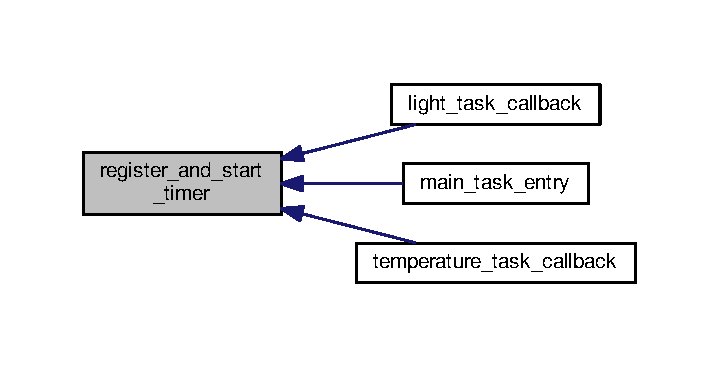
\includegraphics[width=345pt]{common__helper_8h_a23124253b968391b9777fc3b8a0cc5ec_icgraph}
\end{center}
\end{figure}



\hypertarget{error__data_8h}{}\section{/home/gunj/repos/\+E\+C\+E\+N-\/5013/\+Project1/include/common/error\+\_\+data.h File Reference}
\label{error__data_8h}\index{/home/gunj/repos/\+E\+C\+E\+N-\/5013/\+Project1/include/common/error\+\_\+data.\+h@{/home/gunj/repos/\+E\+C\+E\+N-\/5013/\+Project1/include/common/error\+\_\+data.\+h}}
{\ttfamily \#include $<$unistd.\+h$>$}\\*
{\ttfamily \#include $<$sys/syscall.\+h$>$}\\*
{\ttfamily \#include $<$sys/types.\+h$>$}\\*
{\ttfamily \#include $<$stdio.\+h$>$}\\*
Include dependency graph for error\+\_\+data.\+h\+:
\nopagebreak
\begin{figure}[H]
\begin{center}
\leavevmode
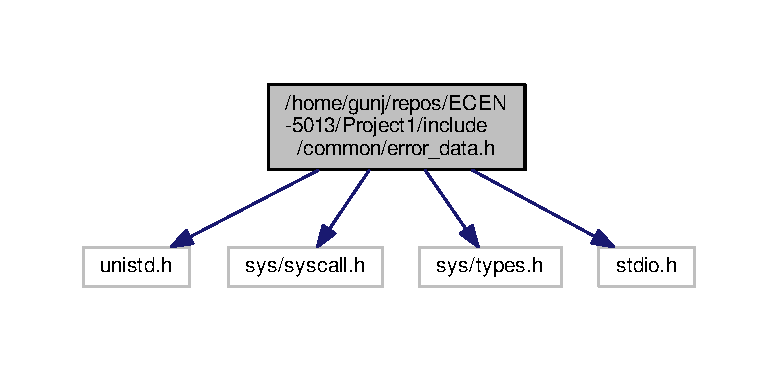
\includegraphics[width=350pt]{error__data_8h__incl}
\end{center}
\end{figure}
This graph shows which files directly or indirectly include this file\+:
\nopagebreak
\begin{figure}[H]
\begin{center}
\leavevmode
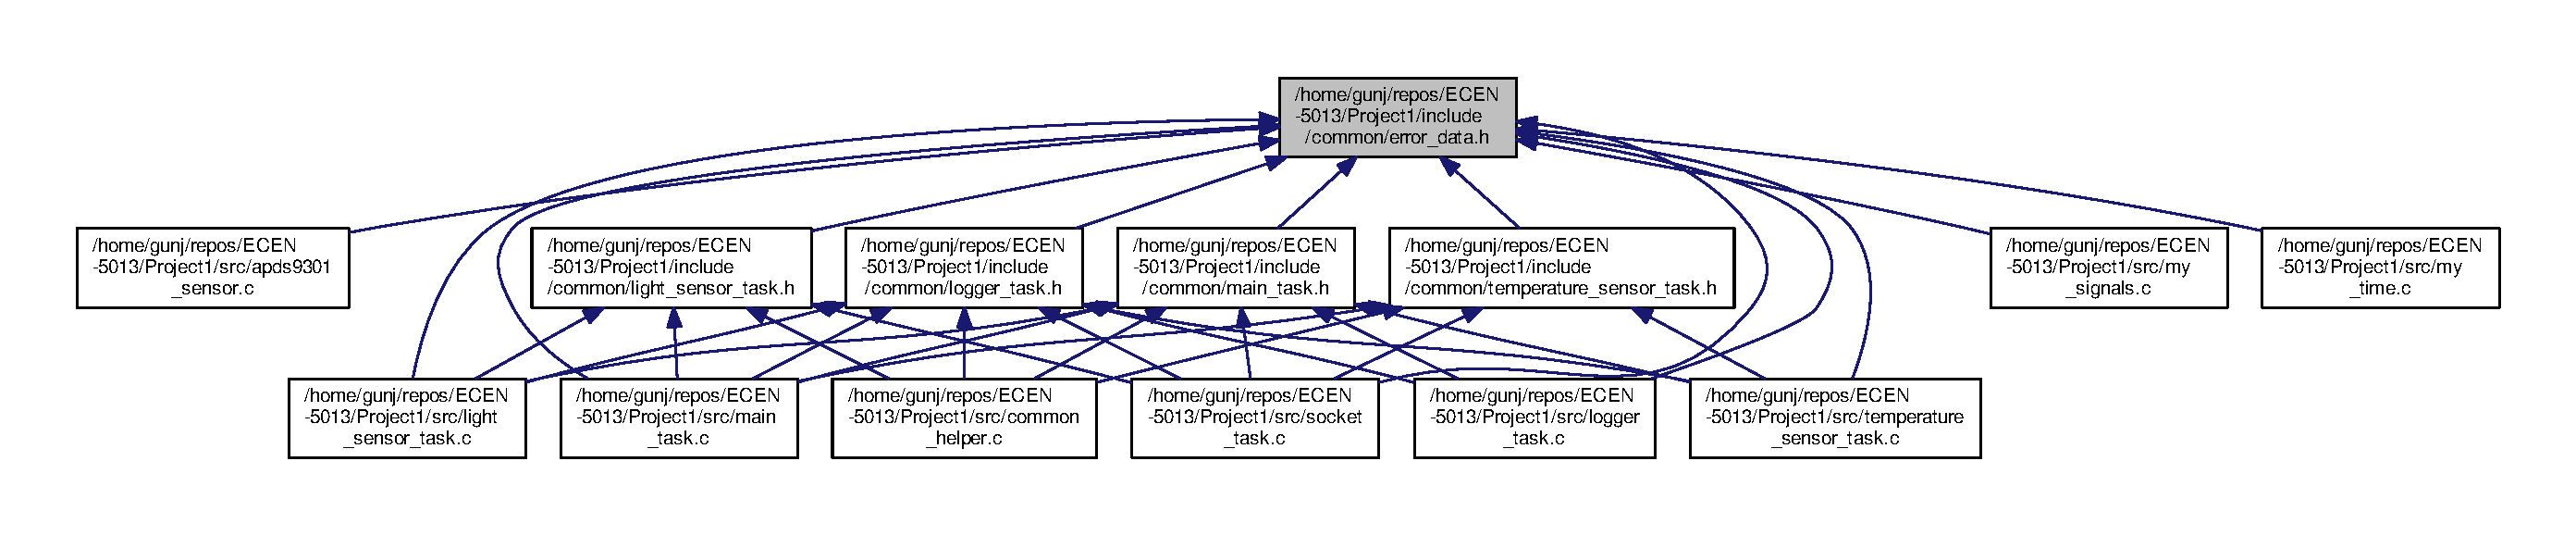
\includegraphics[width=350pt]{error__data_8h__dep__incl}
\end{center}
\end{figure}
\subsection*{Macros}
\begin{DoxyCompactItemize}
\item 
\#define {\bfseries L\+O\+G\+\_\+\+S\+T\+D\+O\+UT}(format, ...)~do\{printf(\char`\"{}\mbox{[}P\+I\+D\+:\%d\mbox{]}\mbox{[}T\+I\+D\+:\%ld\mbox{]}\char`\"{},getpid(),syscall(S\+Y\+S\+\_\+gettid)); printf(format, \#\#\+\_\+\+\_\+\+V\+A\+\_\+\+A\+R\+G\+S\+\_\+\+\_\+); fflush(stdout);\}while(0)\hypertarget{error__data_8h_a8d9af07d8271feb5b31dee7ca2efc611}{}\label{error__data_8h_a8d9af07d8271feb5b31dee7ca2efc611}

\item 
\#define {\bfseries E\+R\+R\+OR}~\char`\"{}\mbox{[}E\+R\+R\+OR\mbox{]} \char`\"{}\hypertarget{error__data_8h_a8fe83ac76edc595f6b98cd4a4127aed5}{}\label{error__data_8h_a8fe83ac76edc595f6b98cd4a4127aed5}

\item 
\#define {\bfseries I\+N\+FO}~\char`\"{}\mbox{[}I\+N\+FO\mbox{]} \char`\"{}\hypertarget{error__data_8h_ae1103fea1e1b3c41ca3322d5389f7162}{}\label{error__data_8h_ae1103fea1e1b3c41ca3322d5389f7162}

\item 
\#define {\bfseries S\+I\+G\+N\+AL}~\char`\"{}\mbox{[}S\+I\+G\+N\+AL\mbox{]} \char`\"{}\hypertarget{error__data_8h_a4688695205ef66fbf096f1b95a0d7fe9}{}\label{error__data_8h_a4688695205ef66fbf096f1b95a0d7fe9}

\item 
\#define {\bfseries W\+A\+R\+N\+I\+NG}~\char`\"{}\mbox{[}W\+A\+R\+N\+I\+NG\mbox{]} \char`\"{}\hypertarget{error__data_8h_a5cb439d9f933fde4cf23caa370c030e7}{}\label{error__data_8h_a5cb439d9f933fde4cf23caa370c030e7}

\end{DoxyCompactItemize}
\subsection*{Enumerations}
\begin{DoxyCompactItemize}
\item 
enum {\bfseries R\+E\+T\+U\+R\+N\+\_\+T} \{ {\bfseries E\+RR} = -\/1, 
{\bfseries S\+U\+C\+C\+E\+SS} = 0
 \}\hypertarget{error__data_8h_a6cbfd0e610bf4b9c5369a3266cb50302}{}\label{error__data_8h_a6cbfd0e610bf4b9c5369a3266cb50302}

\end{DoxyCompactItemize}


\subsection{Detailed Description}
\begin{DoxyAuthor}{Author}
Gunj Manseta 
\end{DoxyAuthor}
\begin{DoxyDate}{Date}
2018-\/03-\/09 
\end{DoxyDate}

\hypertarget{light__sensor__task_8h}{}\section{/home/gunj/repos/\+E\+C\+E\+N-\/5013/\+Project1/include/common/light\+\_\+sensor\+\_\+task.h File Reference}
\label{light__sensor__task_8h}\index{/home/gunj/repos/\+E\+C\+E\+N-\/5013/\+Project1/include/common/light\+\_\+sensor\+\_\+task.\+h@{/home/gunj/repos/\+E\+C\+E\+N-\/5013/\+Project1/include/common/light\+\_\+sensor\+\_\+task.\+h}}
{\ttfamily \#include $<$stdlib.\+h$>$}\\*
{\ttfamily \#include $<$errno.\+h$>$}\\*
{\ttfamily \#include $<$string.\+h$>$}\\*
{\ttfamily \#include $<$mqueue.\+h$>$}\\*
{\ttfamily \#include \char`\"{}common\+\_\+helper.\+h\char`\"{}}\\*
{\ttfamily \#include \char`\"{}my\+\_\+time.\+h\char`\"{}}\\*
{\ttfamily \#include \char`\"{}error\+\_\+data.\+h\char`\"{}}\\*
{\ttfamily \#include \char`\"{}sensor\+\_\+common\+\_\+object.\+h\char`\"{}}\\*
Include dependency graph for light\+\_\+sensor\+\_\+task.\+h\+:\nopagebreak
\begin{figure}[H]
\begin{center}
\leavevmode
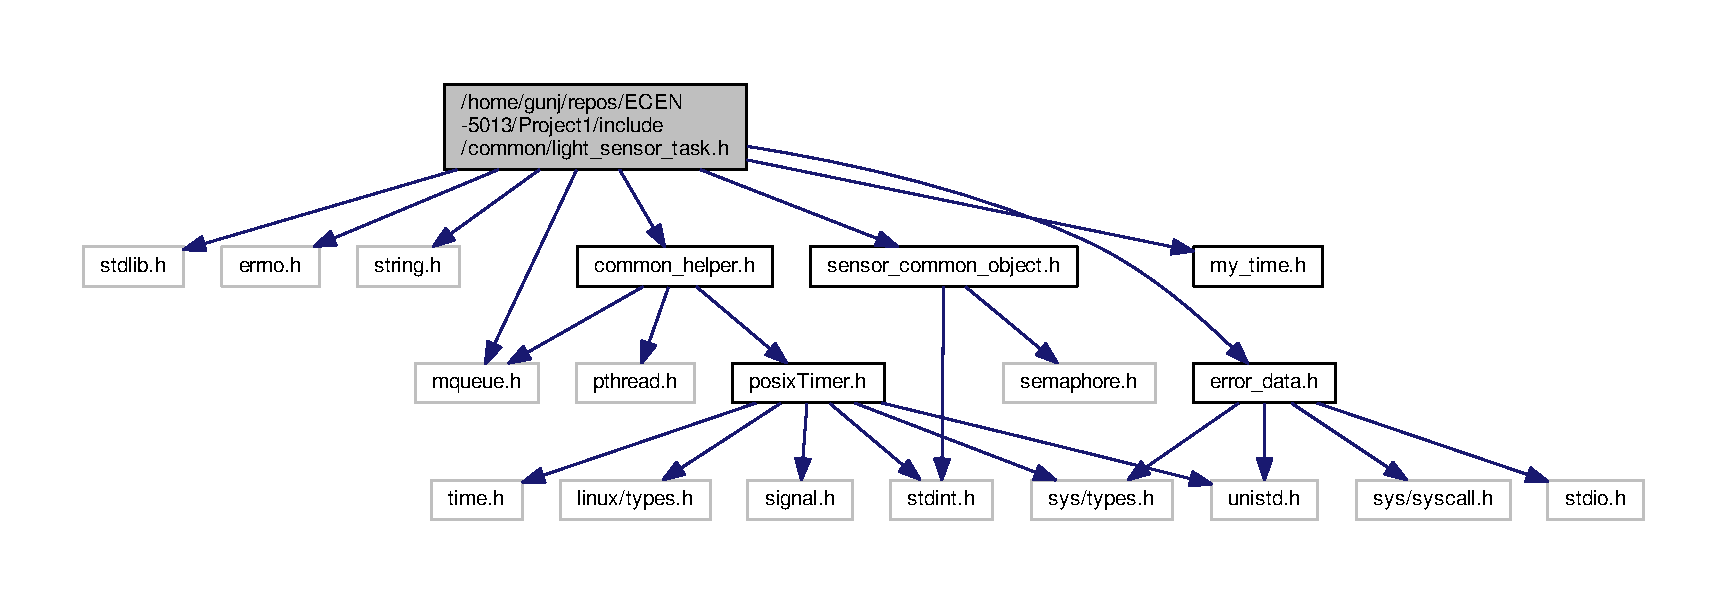
\includegraphics[width=350pt]{light__sensor__task_8h__incl}
\end{center}
\end{figure}
This graph shows which files directly or indirectly include this file\+:\nopagebreak
\begin{figure}[H]
\begin{center}
\leavevmode
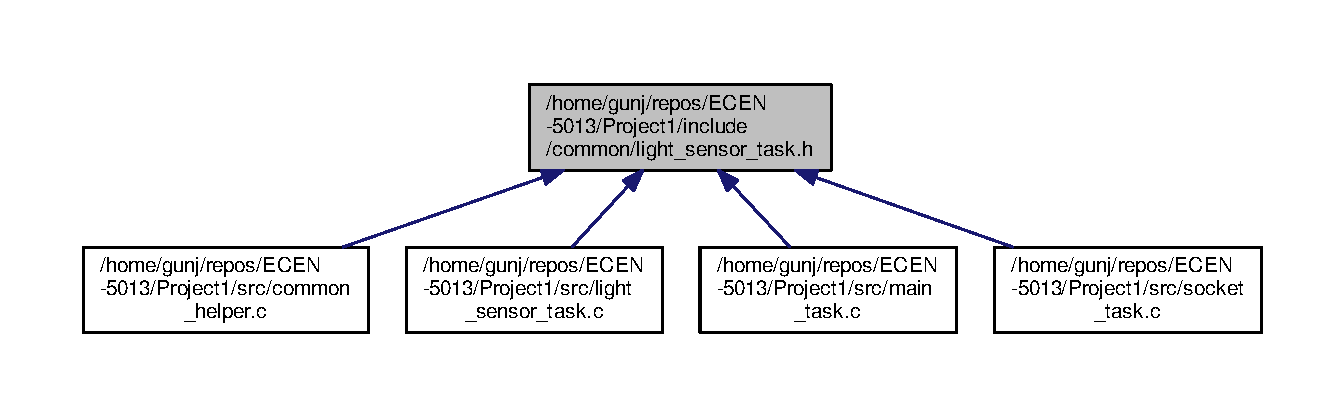
\includegraphics[width=350pt]{light__sensor__task_8h__dep__incl}
\end{center}
\end{figure}
\subsection*{Data Structures}
\begin{DoxyCompactItemize}
\item 
struct \hyperlink{structLIGHTTASKQ__MSG__T}{L\+I\+G\+H\+T\+T\+A\+S\+K\+Q\+\_\+\+M\+S\+G\+\_\+T}
\end{DoxyCompactItemize}
\subsection*{Macros}
\begin{DoxyCompactItemize}
\item 
\#define \hyperlink{light__sensor__task_8h_ad3c64139927109ac2021342f1912828b}{D\+E\+F\+I\+N\+E\+\_\+\+L\+I\+G\+H\+T\+\_\+\+S\+T\+R\+U\+CT}(name,  msg\+Id,  source\+Id)
\begin{DoxyCompactList}\small\item\em Defines a light struct with the name given and params with some default values. \end{DoxyCompactList}\item 
\#define {\bfseries P\+O\+S\+T\+\_\+\+M\+E\+S\+S\+A\+G\+E\+\_\+\+L\+I\+G\+H\+T\+T\+A\+SK}(p\+\_\+lightstruct)
\item 
\#define {\bfseries P\+O\+S\+T\+\_\+\+M\+E\+S\+S\+A\+G\+E\+\_\+\+L\+I\+G\+H\+T\+T\+A\+S\+K\+\_\+\+E\+X\+IT}(p\+\_\+lightstruct)
\end{DoxyCompactItemize}
\subsection*{Enumerations}
\begin{DoxyCompactItemize}
\item 
enum {\bfseries D\+A\+Y\+\_\+\+S\+T\+A\+T\+E\+\_\+T} \{ {\bfseries D\+AY} = 0, 
{\bfseries N\+I\+G\+HT} = 1
 \}\hypertarget{light__sensor__task_8h_a7d714c313df3e00dc24e02490e1c4c08}{}\label{light__sensor__task_8h_a7d714c313df3e00dc24e02490e1c4c08}

\item 
enum {\bfseries L\+I\+G\+H\+T\+T\+A\+S\+K\+Q\+\_\+\+M\+S\+G\+I\+D\+\_\+T} \{ \\*
{\bfseries L\+I\+G\+H\+T\+\_\+\+M\+S\+G\+\_\+\+T\+A\+S\+K\+\_\+\+S\+T\+A\+T\+US}, 
{\bfseries L\+I\+G\+H\+T\+\_\+\+M\+S\+G\+\_\+\+T\+A\+S\+K\+\_\+\+G\+E\+T\+\_\+\+S\+T\+A\+TE}, 
{\bfseries L\+I\+G\+H\+T\+\_\+\+M\+S\+G\+\_\+\+T\+A\+S\+K\+\_\+\+R\+E\+A\+D\+\_\+\+D\+A\+TA}, 
{\bfseries L\+I\+G\+H\+T\+\_\+\+M\+S\+G\+\_\+\+T\+A\+S\+K\+\_\+\+W\+R\+I\+T\+E\+\_\+\+C\+MD}, 
\\*
{\bfseries L\+I\+G\+H\+T\+\_\+\+M\+S\+G\+\_\+\+T\+A\+S\+K\+\_\+\+P\+O\+W\+E\+R\+D\+O\+WN}, 
{\bfseries L\+I\+G\+H\+T\+\_\+\+M\+S\+G\+\_\+\+T\+A\+S\+K\+\_\+\+P\+O\+W\+E\+R\+UP}, 
{\bfseries L\+I\+G\+H\+T\+\_\+\+M\+S\+G\+\_\+\+T\+A\+S\+K\+\_\+\+E\+X\+IT}
 \}\hypertarget{light__sensor__task_8h_ab864429fd48fdeac96f07665a36779f1}{}\label{light__sensor__task_8h_ab864429fd48fdeac96f07665a36779f1}

\end{DoxyCompactItemize}
\subsection*{Functions}
\begin{DoxyCompactItemize}
\item 
mqd\+\_\+t \hyperlink{light__sensor__task_8h_ace4b0c78a43f482e74bc1d7a717c753c}{get\+Handle\+\_\+\+Light\+Task\+Queue} ()
\begin{DoxyCompactList}\small\item\em Get the Handle Light\+Task\+Queue object. \end{DoxyCompactList}\item 
D\+A\+Y\+\_\+\+S\+T\+A\+T\+E\+\_\+T \hyperlink{light__sensor__task_8h_a2fb8d8bd6f3ac82658743d379b205a51}{get\+Light\+Task\+\_\+state} ()
\begin{DoxyCompactList}\small\item\em Get the Light\+Task state object M\+T-\/safe. \end{DoxyCompactList}\item 
float \hyperlink{light__sensor__task_8h_ac88a5567bdeac532053519330e94c6ab}{get\+Light\+Task\+\_\+lux} ()
\begin{DoxyCompactList}\small\item\em Get the Light\+Task lux object. M\+T-\/safe as it calls a M\+T-\/safe function within. \end{DoxyCompactList}\item 
void $\ast$ \hyperlink{light__sensor__task_8h_a638f4ba787ad818d90477af9e572771c}{light\+\_\+task\+\_\+callback} (void $\ast$threadparam)
\begin{DoxyCompactList}\small\item\em Entry point of the light task thread. \end{DoxyCompactList}\end{DoxyCompactItemize}


\subsection{Detailed Description}
\begin{DoxyAuthor}{Author}
Gunj Manseta 
\end{DoxyAuthor}
\begin{DoxyDate}{Date}
2018-\/03-\/11 
\end{DoxyDate}


\subsection{Macro Definition Documentation}
\index{light\+\_\+sensor\+\_\+task.\+h@{light\+\_\+sensor\+\_\+task.\+h}!D\+E\+F\+I\+N\+E\+\_\+\+L\+I\+G\+H\+T\+\_\+\+S\+T\+R\+U\+CT@{D\+E\+F\+I\+N\+E\+\_\+\+L\+I\+G\+H\+T\+\_\+\+S\+T\+R\+U\+CT}}
\index{D\+E\+F\+I\+N\+E\+\_\+\+L\+I\+G\+H\+T\+\_\+\+S\+T\+R\+U\+CT@{D\+E\+F\+I\+N\+E\+\_\+\+L\+I\+G\+H\+T\+\_\+\+S\+T\+R\+U\+CT}!light\+\_\+sensor\+\_\+task.\+h@{light\+\_\+sensor\+\_\+task.\+h}}
\subsubsection[{\texorpdfstring{D\+E\+F\+I\+N\+E\+\_\+\+L\+I\+G\+H\+T\+\_\+\+S\+T\+R\+U\+CT}{DEFINE_LIGHT_STRUCT}}]{\setlength{\rightskip}{0pt plus 5cm}\#define D\+E\+F\+I\+N\+E\+\_\+\+L\+I\+G\+H\+T\+\_\+\+S\+T\+R\+U\+CT(
\begin{DoxyParamCaption}
\item[{}]{name, }
\item[{}]{msg\+Id, }
\item[{}]{source\+Id}
\end{DoxyParamCaption}
)}\hypertarget{light__sensor__task_8h_ad3c64139927109ac2021342f1912828b}{}\label{light__sensor__task_8h_ad3c64139927109ac2021342f1912828b}
{\bfseries Value\+:}
\begin{DoxyCode}
\hyperlink{structLIGHTTASKQ__MSG__T}{LIGHTTASKQ\_MSG\_T} name = \{      \(\backslash\)
        .msgID      = msgId,        \(\backslash\)
        .sourceID   = sourceId,     \(\backslash\)
        .packet     = \{0\}           \(\backslash\)
    \};
\end{DoxyCode}


Defines a light struct with the name given and params with some default values. 

\index{light\+\_\+sensor\+\_\+task.\+h@{light\+\_\+sensor\+\_\+task.\+h}!P\+O\+S\+T\+\_\+\+M\+E\+S\+S\+A\+G\+E\+\_\+\+L\+I\+G\+H\+T\+T\+A\+SK@{P\+O\+S\+T\+\_\+\+M\+E\+S\+S\+A\+G\+E\+\_\+\+L\+I\+G\+H\+T\+T\+A\+SK}}
\index{P\+O\+S\+T\+\_\+\+M\+E\+S\+S\+A\+G\+E\+\_\+\+L\+I\+G\+H\+T\+T\+A\+SK@{P\+O\+S\+T\+\_\+\+M\+E\+S\+S\+A\+G\+E\+\_\+\+L\+I\+G\+H\+T\+T\+A\+SK}!light\+\_\+sensor\+\_\+task.\+h@{light\+\_\+sensor\+\_\+task.\+h}}
\subsubsection[{\texorpdfstring{P\+O\+S\+T\+\_\+\+M\+E\+S\+S\+A\+G\+E\+\_\+\+L\+I\+G\+H\+T\+T\+A\+SK}{POST_MESSAGE_LIGHTTASK}}]{\setlength{\rightskip}{0pt plus 5cm}\#define P\+O\+S\+T\+\_\+\+M\+E\+S\+S\+A\+G\+E\+\_\+\+L\+I\+G\+H\+T\+T\+A\+SK(
\begin{DoxyParamCaption}
\item[{}]{p\+\_\+lightstruct}
\end{DoxyParamCaption}
)}\hypertarget{light__sensor__task_8h_ae936fca69f20a6a81f530eb38806bd3c}{}\label{light__sensor__task_8h_ae936fca69f20a6a81f530eb38806bd3c}
{\bfseries Value\+:}
\begin{DoxyCode}
\textcolor{keywordflow}{do}\{ \(\backslash\)
        \_\_POST\_MESSAGE\_LIGHTTASK(\hyperlink{light__sensor__task_8h_ace4b0c78a43f482e74bc1d7a717c753c}{getHandle\_LightTaskQueue}(), p\_lightstruct, \textcolor{keyword}{sizeof}(
      *p\_lightstruct),20); \(\backslash\)
    \}\textcolor{keywordflow}{while}(0)
\end{DoxyCode}
\index{light\+\_\+sensor\+\_\+task.\+h@{light\+\_\+sensor\+\_\+task.\+h}!P\+O\+S\+T\+\_\+\+M\+E\+S\+S\+A\+G\+E\+\_\+\+L\+I\+G\+H\+T\+T\+A\+S\+K\+\_\+\+E\+X\+IT@{P\+O\+S\+T\+\_\+\+M\+E\+S\+S\+A\+G\+E\+\_\+\+L\+I\+G\+H\+T\+T\+A\+S\+K\+\_\+\+E\+X\+IT}}
\index{P\+O\+S\+T\+\_\+\+M\+E\+S\+S\+A\+G\+E\+\_\+\+L\+I\+G\+H\+T\+T\+A\+S\+K\+\_\+\+E\+X\+IT@{P\+O\+S\+T\+\_\+\+M\+E\+S\+S\+A\+G\+E\+\_\+\+L\+I\+G\+H\+T\+T\+A\+S\+K\+\_\+\+E\+X\+IT}!light\+\_\+sensor\+\_\+task.\+h@{light\+\_\+sensor\+\_\+task.\+h}}
\subsubsection[{\texorpdfstring{P\+O\+S\+T\+\_\+\+M\+E\+S\+S\+A\+G\+E\+\_\+\+L\+I\+G\+H\+T\+T\+A\+S\+K\+\_\+\+E\+X\+IT}{POST_MESSAGE_LIGHTTASK_EXIT}}]{\setlength{\rightskip}{0pt plus 5cm}\#define P\+O\+S\+T\+\_\+\+M\+E\+S\+S\+A\+G\+E\+\_\+\+L\+I\+G\+H\+T\+T\+A\+S\+K\+\_\+\+E\+X\+IT(
\begin{DoxyParamCaption}
\item[{}]{p\+\_\+lightstruct}
\end{DoxyParamCaption}
)}\hypertarget{light__sensor__task_8h_abafa6c4697460e4887f6d6e9c1f15749}{}\label{light__sensor__task_8h_abafa6c4697460e4887f6d6e9c1f15749}
{\bfseries Value\+:}
\begin{DoxyCode}
\textcolor{keywordflow}{do}\{ \(\backslash\)
        \_\_POST\_MESSAGE\_LIGHTTASK(\hyperlink{light__sensor__task_8h_ace4b0c78a43f482e74bc1d7a717c753c}{getHandle\_LightTaskQueue}(), p\_lightstruct, \textcolor{keyword}{sizeof}(
      *p\_lightstruct),50); \(\backslash\)
    \}\textcolor{keywordflow}{while}(0)
\end{DoxyCode}


\subsection{Function Documentation}
\index{light\+\_\+sensor\+\_\+task.\+h@{light\+\_\+sensor\+\_\+task.\+h}!get\+Handle\+\_\+\+Light\+Task\+Queue@{get\+Handle\+\_\+\+Light\+Task\+Queue}}
\index{get\+Handle\+\_\+\+Light\+Task\+Queue@{get\+Handle\+\_\+\+Light\+Task\+Queue}!light\+\_\+sensor\+\_\+task.\+h@{light\+\_\+sensor\+\_\+task.\+h}}
\subsubsection[{\texorpdfstring{get\+Handle\+\_\+\+Light\+Task\+Queue()}{getHandle_LightTaskQueue()}}]{\setlength{\rightskip}{0pt plus 5cm}mqd\+\_\+t get\+Handle\+\_\+\+Light\+Task\+Queue (
\begin{DoxyParamCaption}
{}
\end{DoxyParamCaption}
)}\hypertarget{light__sensor__task_8h_ace4b0c78a43f482e74bc1d7a717c753c}{}\label{light__sensor__task_8h_ace4b0c78a43f482e74bc1d7a717c753c}


Get the Handle Light\+Task\+Queue object. 

\begin{DoxyReturn}{Returns}
mqd\+\_\+t 
\end{DoxyReturn}

\begin{DoxyCode}
86 \{
87     \textcolor{keywordflow}{return} lighttask\_q;
88 \}
\end{DoxyCode}
\index{light\+\_\+sensor\+\_\+task.\+h@{light\+\_\+sensor\+\_\+task.\+h}!get\+Light\+Task\+\_\+lux@{get\+Light\+Task\+\_\+lux}}
\index{get\+Light\+Task\+\_\+lux@{get\+Light\+Task\+\_\+lux}!light\+\_\+sensor\+\_\+task.\+h@{light\+\_\+sensor\+\_\+task.\+h}}
\subsubsection[{\texorpdfstring{get\+Light\+Task\+\_\+lux()}{getLightTask_lux()}}]{\setlength{\rightskip}{0pt plus 5cm}float get\+Light\+Task\+\_\+lux (
\begin{DoxyParamCaption}
{}
\end{DoxyParamCaption}
)}\hypertarget{light__sensor__task_8h_ac88a5567bdeac532053519330e94c6ab}{}\label{light__sensor__task_8h_ac88a5567bdeac532053519330e94c6ab}


Get the Light\+Task lux object. M\+T-\/safe as it calls a M\+T-\/safe function within. 

\begin{DoxyReturn}{Returns}
float 
\end{DoxyReturn}

\begin{DoxyCode}
46 \{
47     \textcolor{keywordtype}{float} lux = \hyperlink{apds9301__sensor_8c_a55e164e7dd0586de71a8dd5b25ae9ef3}{APDS9301\_getLux}();
48     \textcolor{keywordflow}{return} lux;
49 \}
\end{DoxyCode}


Here is the caller graph for this function\+:\nopagebreak
\begin{figure}[H]
\begin{center}
\leavevmode
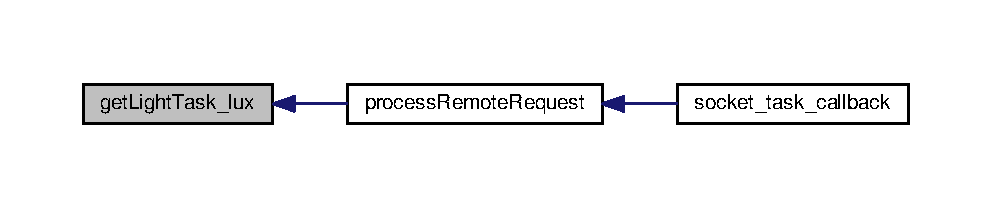
\includegraphics[width=350pt]{light__sensor__task_8h_ac88a5567bdeac532053519330e94c6ab_icgraph}
\end{center}
\end{figure}


\index{light\+\_\+sensor\+\_\+task.\+h@{light\+\_\+sensor\+\_\+task.\+h}!get\+Light\+Task\+\_\+state@{get\+Light\+Task\+\_\+state}}
\index{get\+Light\+Task\+\_\+state@{get\+Light\+Task\+\_\+state}!light\+\_\+sensor\+\_\+task.\+h@{light\+\_\+sensor\+\_\+task.\+h}}
\subsubsection[{\texorpdfstring{get\+Light\+Task\+\_\+state()}{getLightTask_state()}}]{\setlength{\rightskip}{0pt plus 5cm}D\+A\+Y\+\_\+\+S\+T\+A\+T\+E\+\_\+T get\+Light\+Task\+\_\+state (
\begin{DoxyParamCaption}
{}
\end{DoxyParamCaption}
)}\hypertarget{light__sensor__task_8h_a2fb8d8bd6f3ac82658743d379b205a51}{}\label{light__sensor__task_8h_a2fb8d8bd6f3ac82658743d379b205a51}


Get the Light\+Task state object M\+T-\/safe. 

\begin{DoxyReturn}{Returns}
D\+A\+Y\+\_\+\+S\+T\+A\+T\+E\+\_\+T 
\end{DoxyReturn}

\begin{DoxyCode}
37 \{
38     DAY\_STATE\_T state;
39     pthread\_mutex\_lock(&stateChangeLock);
40     state = isDay;
41     pthread\_mutex\_unlock(&stateChangeLock);
42     \textcolor{keywordflow}{return} state;
43 \}
\end{DoxyCode}


Here is the caller graph for this function\+:\nopagebreak
\begin{figure}[H]
\begin{center}
\leavevmode
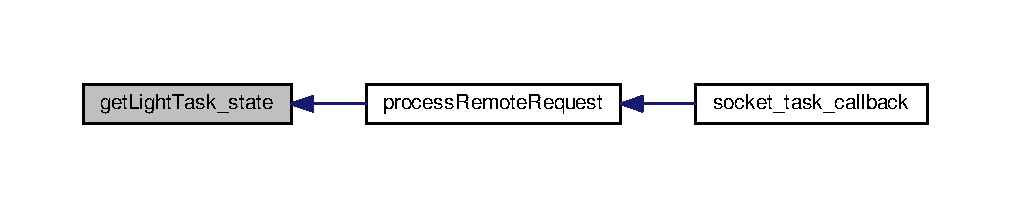
\includegraphics[width=350pt]{light__sensor__task_8h_a2fb8d8bd6f3ac82658743d379b205a51_icgraph}
\end{center}
\end{figure}


\index{light\+\_\+sensor\+\_\+task.\+h@{light\+\_\+sensor\+\_\+task.\+h}!light\+\_\+task\+\_\+callback@{light\+\_\+task\+\_\+callback}}
\index{light\+\_\+task\+\_\+callback@{light\+\_\+task\+\_\+callback}!light\+\_\+sensor\+\_\+task.\+h@{light\+\_\+sensor\+\_\+task.\+h}}
\subsubsection[{\texorpdfstring{light\+\_\+task\+\_\+callback(void $\ast$threadparam)}{light_task_callback(void *threadparam)}}]{\setlength{\rightskip}{0pt plus 5cm}void$\ast$ light\+\_\+task\+\_\+callback (
\begin{DoxyParamCaption}
\item[{void $\ast$}]{threadparam}
\end{DoxyParamCaption}
)}\hypertarget{light__sensor__task_8h_a638f4ba787ad818d90477af9e572771c}{}\label{light__sensor__task_8h_a638f4ba787ad818d90477af9e572771c}


Entry point of the light task thread. 


\begin{DoxyParams}{Parameters}
{\em threadparam} & \\
\hline
\end{DoxyParams}
\begin{DoxyReturn}{Returns}
void$\ast$ 
\end{DoxyReturn}

\begin{DoxyCode}
204 \{
205     LOG\_STDOUT(INFO \textcolor{stringliteral}{"LIGHT TASK STARTED\(\backslash\)n"});
206 
207     \textcolor{keywordtype}{int} ret = \hyperlink{light__sensor__task_8c_abb5f74ca3376b1b610b7dac47ecae8d8}{light\_task\_queue\_init}();
208     \textcolor{keywordflow}{if}(ERR == ret)
209     \{
210         LOG\_STDOUT(ERROR \textcolor{stringliteral}{"LIGHT TASK QUEUE INIT:%s\(\backslash\)n"},strerror(errno));
211         exit(ERR);
212     \}
213 
214     \hyperlink{structi2c__handle}{I2C\_MASTER\_HANDLE\_T} i2c;
215     ret = light\_task\_sensorUP(&i2c);
216     \textcolor{keywordflow}{if}(ERR == ret)
217     \{
218         LOG\_STDOUT(ERROR \textcolor{stringliteral}{"LIGHT TASK SENSOR INIT:%s\(\backslash\)n"},strerror(errno));
219         \textcolor{keywordflow}{goto} FAIL\_EXIT\_SENSOR;
220     \}
221 
222     
223     LOG\_STDOUT(INFO \textcolor{stringliteral}{"[OK] LIGHT TASK INIT COMPLETED\(\backslash\)n"});
224     pthread\_barrier\_wait(&tasks\_barrier);
225 
226     \textcolor{comment}{/* Registering a timer for 2 sec to update the state of the snesor value by getting the lux value from
       the sensor*/}
227     timer\_t timer\_id;
228     \textcolor{keywordflow}{if}(ERR == \hyperlink{common__helper_8c_a23124253b968391b9777fc3b8a0cc5ec}{register\_and\_start\_timer}(&timer\_id, 2*MICROSEC, 0, 
      timer\_handler\_getAndUpdateState, &timer\_id))
229     \{
230         \textcolor{comment}{// LOG\_STDOUT(ERROR "Timer Error\(\backslash\)n");}
231         \textcolor{keywordflow}{goto} FAIL\_EXIT;
232     \}
233 
234     \textcolor{comment}{/* Process Log queue msg which executes untill the log\_task\_end flag is set to true*/}
235     light\_task\_processMsg();
236 
237     ret = \hyperlink{posixTimer_8c_a91f15230e46caba2a2132b04e9c73e47}{delete\_timer}(timer\_id);
238     \textcolor{keywordflow}{if}(ERR == ret)
239     \{
240         LOG\_STDOUT(ERROR \textcolor{stringliteral}{"LIGHT TASK DELETE TIMER:%s\(\backslash\)n"},strerror(errno));
241     \}
242 
243 FAIL\_EXIT:
244 
245     light\_task\_sensorDOWN(&i2c);
246 
247 FAIL\_EXIT\_SENSOR:
248     mq\_close(lighttask\_q);
249     LOG\_STDOUT(INFO \textcolor{stringliteral}{"Light task exit.\(\backslash\)n"});
250     \textcolor{keywordflow}{return} SUCCESS;
251 \}\end{DoxyCode}

\hypertarget{logger__task_8h}{}\section{/home/gunj/repos/\+E\+C\+E\+N-\/5013/\+Project1/include/common/logger\+\_\+task.h File Reference}
\label{logger__task_8h}\index{/home/gunj/repos/\+E\+C\+E\+N-\/5013/\+Project1/include/common/logger\+\_\+task.\+h@{/home/gunj/repos/\+E\+C\+E\+N-\/5013/\+Project1/include/common/logger\+\_\+task.\+h}}
{\ttfamily \#include $<$stdlib.\+h$>$}\\*
{\ttfamily \#include $<$errno.\+h$>$}\\*
{\ttfamily \#include $<$string.\+h$>$}\\*
{\ttfamily \#include $<$mqueue.\+h$>$}\\*
{\ttfamily \#include \char`\"{}common\+\_\+helper.\+h\char`\"{}}\\*
{\ttfamily \#include \char`\"{}my\+\_\+time.\+h\char`\"{}}\\*
{\ttfamily \#include \char`\"{}error\+\_\+data.\+h\char`\"{}}\\*
Include dependency graph for logger\+\_\+task.\+h\+:\nopagebreak
\begin{figure}[H]
\begin{center}
\leavevmode
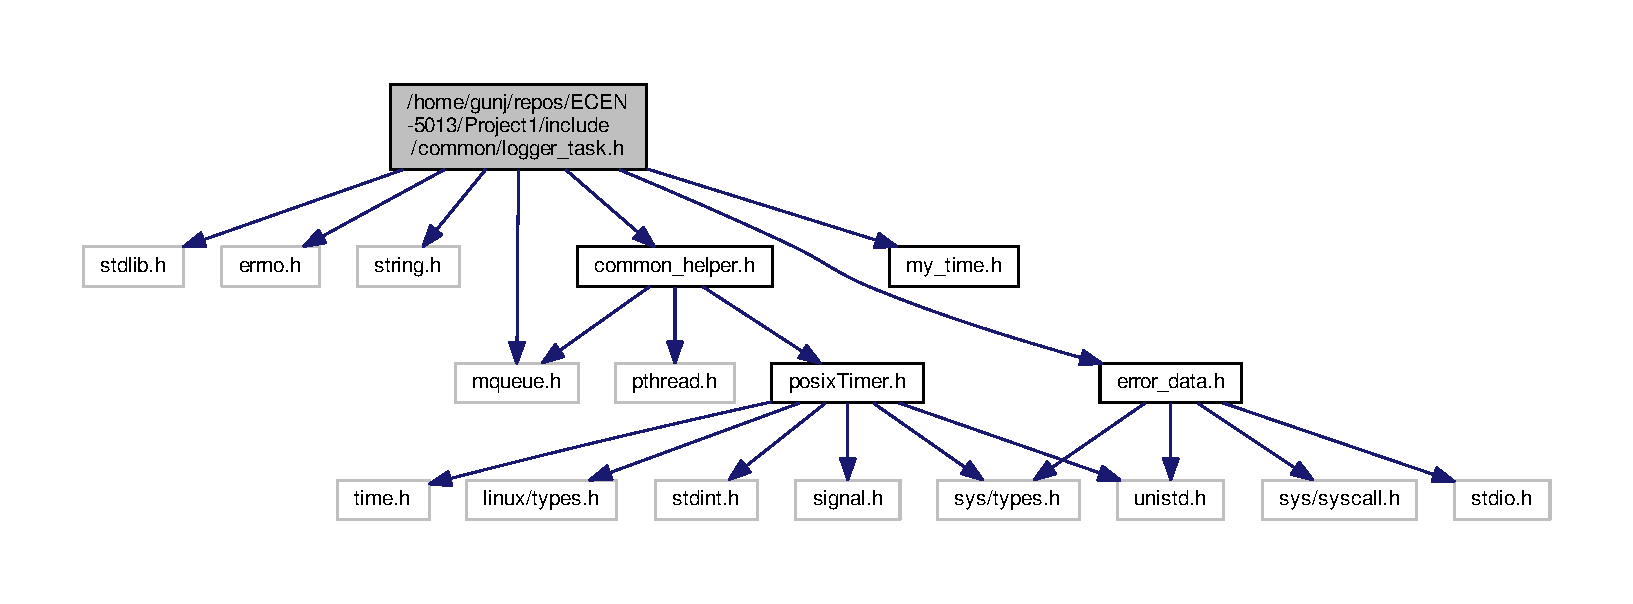
\includegraphics[width=350pt]{logger__task_8h__incl}
\end{center}
\end{figure}
This graph shows which files directly or indirectly include this file\+:\nopagebreak
\begin{figure}[H]
\begin{center}
\leavevmode
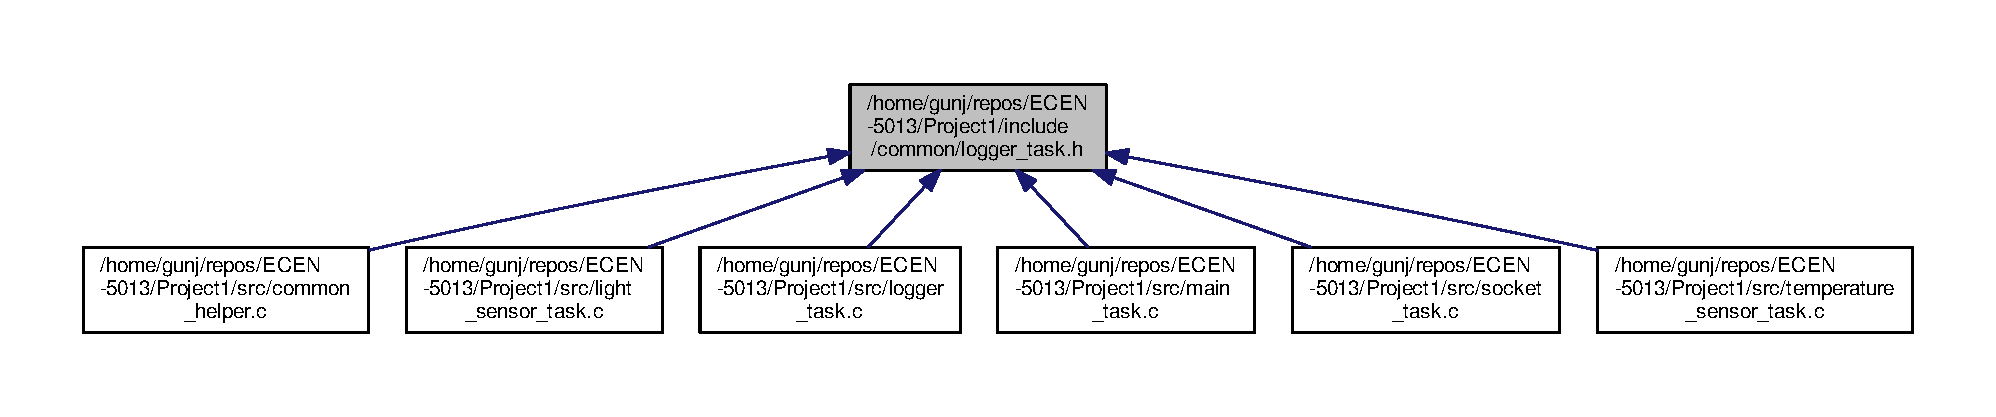
\includegraphics[width=350pt]{logger__task_8h__dep__incl}
\end{center}
\end{figure}
\subsection*{Data Structures}
\begin{DoxyCompactItemize}
\item 
struct \hyperlink{structLOGGERTASKQ__MSG__T}{L\+O\+G\+G\+E\+R\+T\+A\+S\+K\+Q\+\_\+\+M\+S\+G\+\_\+T}
\end{DoxyCompactItemize}
\subsection*{Macros}
\begin{DoxyCompactItemize}
\item 
\#define {\bfseries L\+T\+\_\+\+M\+S\+G\+\_\+\+S\+I\+ZE}~40\hypertarget{logger__task_8h_a3e0953f6f3a48d888c4966ec9d77eb47}{}\label{logger__task_8h_a3e0953f6f3a48d888c4966ec9d77eb47}

\item 
\#define \hyperlink{logger__task_8h_a006cfbef67bbc2a8a43363fb6aab41e9}{D\+E\+F\+I\+N\+E\+\_\+\+L\+O\+G\+\_\+\+S\+T\+R\+U\+CT}(name,  msg\+Id,  source\+Id)
\begin{DoxyCompactList}\small\item\em Defines a Log struct with the name given and params with some default values. \end{DoxyCompactList}\item 
\#define {\bfseries P\+O\+S\+T\+\_\+\+M\+E\+S\+S\+A\+G\+E\+\_\+\+L\+O\+G\+T\+A\+SK}(p\+\_\+logstruct,  format, ...)
\item 
\#define {\bfseries P\+O\+S\+T\+\_\+\+M\+E\+S\+S\+A\+G\+E\+\_\+\+L\+O\+G\+T\+A\+S\+K\+\_\+\+E\+X\+IT}(p\+\_\+logstruct,  format, ...)
\end{DoxyCompactItemize}
\subsection*{Typedefs}
\begin{DoxyCompactItemize}
\item 
typedef char {\bfseries L\+O\+G\+G\+E\+R\+\_\+\+T\+A\+S\+K\+\_\+\+M\+S\+G\+D\+A\+T\+A\+\_\+T}\hypertarget{logger__task_8h_a2d188b418a97bc2072c76cebf414a3a6}{}\label{logger__task_8h_a2d188b418a97bc2072c76cebf414a3a6}

\end{DoxyCompactItemize}
\subsection*{Enumerations}
\begin{DoxyCompactItemize}
\item 
enum {\bfseries L\+O\+G\+G\+E\+R\+T\+A\+S\+K\+Q\+\_\+\+M\+S\+G\+I\+D\+\_\+T} \{ {\bfseries L\+T\+\_\+\+M\+S\+G\+\_\+\+T\+A\+S\+K\+\_\+\+S\+T\+A\+T\+US}, 
{\bfseries L\+T\+\_\+\+M\+S\+G\+\_\+\+L\+OG}, 
{\bfseries L\+T\+\_\+\+M\+S\+G\+\_\+\+T\+A\+S\+K\+\_\+\+E\+X\+IT}
 \}\hypertarget{logger__task_8h_a94334c0c387ff34c6a268ee8ee6028ad}{}\label{logger__task_8h_a94334c0c387ff34c6a268ee8ee6028ad}

\item 
enum {\bfseries L\+O\+G\+\_\+\+L\+E\+V\+E\+L\+\_\+T} \{ {\bfseries L\+O\+G\+\_\+\+E\+R\+R\+OR}, 
{\bfseries L\+O\+G\+\_\+\+W\+A\+R\+N\+I\+NG}, 
{\bfseries L\+O\+G\+\_\+\+I\+N\+FO}, 
{\bfseries L\+O\+G\+\_\+\+A\+LL}
 \}\hypertarget{logger__task_8h_aecf2a701f46029451c8733fde5134a89}{}\label{logger__task_8h_aecf2a701f46029451c8733fde5134a89}

\end{DoxyCompactItemize}
\subsection*{Functions}
\begin{DoxyCompactItemize}
\item 
mqd\+\_\+t \hyperlink{logger__task_8h_ac3b7cda92012133de3b948c721737097}{get\+Handle\+\_\+\+Logger\+Task\+Queue} ()
\begin{DoxyCompactList}\small\item\em Get the Handle Logger\+Task\+Queue object. \end{DoxyCompactList}\item 
void $\ast$ \hyperlink{logger__task_8h_a7322e57eb5c8763112ad4d4a946601bf}{logger\+\_\+task\+\_\+callback} (void $\ast$threadparam)
\begin{DoxyCompactList}\small\item\em Entry point of the logger task thread. \end{DoxyCompactList}\end{DoxyCompactItemize}


\subsection{Detailed Description}
\begin{DoxyAuthor}{Author}
Gunj Manseta 
\end{DoxyAuthor}
\begin{DoxyDate}{Date}
2018-\/03-\/09 
\end{DoxyDate}


\subsection{Macro Definition Documentation}
\index{logger\+\_\+task.\+h@{logger\+\_\+task.\+h}!D\+E\+F\+I\+N\+E\+\_\+\+L\+O\+G\+\_\+\+S\+T\+R\+U\+CT@{D\+E\+F\+I\+N\+E\+\_\+\+L\+O\+G\+\_\+\+S\+T\+R\+U\+CT}}
\index{D\+E\+F\+I\+N\+E\+\_\+\+L\+O\+G\+\_\+\+S\+T\+R\+U\+CT@{D\+E\+F\+I\+N\+E\+\_\+\+L\+O\+G\+\_\+\+S\+T\+R\+U\+CT}!logger\+\_\+task.\+h@{logger\+\_\+task.\+h}}
\subsubsection[{\texorpdfstring{D\+E\+F\+I\+N\+E\+\_\+\+L\+O\+G\+\_\+\+S\+T\+R\+U\+CT}{DEFINE_LOG_STRUCT}}]{\setlength{\rightskip}{0pt plus 5cm}\#define D\+E\+F\+I\+N\+E\+\_\+\+L\+O\+G\+\_\+\+S\+T\+R\+U\+CT(
\begin{DoxyParamCaption}
\item[{}]{name, }
\item[{}]{msg\+Id, }
\item[{}]{source\+Id}
\end{DoxyParamCaption}
)}\hypertarget{logger__task_8h_a006cfbef67bbc2a8a43363fb6aab41e9}{}\label{logger__task_8h_a006cfbef67bbc2a8a43363fb6aab41e9}
{\bfseries Value\+:}
\begin{DoxyCode}
\hyperlink{structLOGGERTASKQ__MSG__T}{LOGGERTASKQ\_MSG\_T} name = \{      \(\backslash\)
        .msgID      = msgId,        \(\backslash\)
        .loglevel   = LOG\_ALL,      \(\backslash\)
        .sourceID   = sourceId,     \(\backslash\)
        .timestamp  = \{0\},          \(\backslash\)
        .msgData    = \{0\}           \(\backslash\)
    \};
\end{DoxyCode}


Defines a Log struct with the name given and params with some default values. 

\index{logger\+\_\+task.\+h@{logger\+\_\+task.\+h}!P\+O\+S\+T\+\_\+\+M\+E\+S\+S\+A\+G\+E\+\_\+\+L\+O\+G\+T\+A\+SK@{P\+O\+S\+T\+\_\+\+M\+E\+S\+S\+A\+G\+E\+\_\+\+L\+O\+G\+T\+A\+SK}}
\index{P\+O\+S\+T\+\_\+\+M\+E\+S\+S\+A\+G\+E\+\_\+\+L\+O\+G\+T\+A\+SK@{P\+O\+S\+T\+\_\+\+M\+E\+S\+S\+A\+G\+E\+\_\+\+L\+O\+G\+T\+A\+SK}!logger\+\_\+task.\+h@{logger\+\_\+task.\+h}}
\subsubsection[{\texorpdfstring{P\+O\+S\+T\+\_\+\+M\+E\+S\+S\+A\+G\+E\+\_\+\+L\+O\+G\+T\+A\+SK}{POST_MESSAGE_LOGTASK}}]{\setlength{\rightskip}{0pt plus 5cm}\#define P\+O\+S\+T\+\_\+\+M\+E\+S\+S\+A\+G\+E\+\_\+\+L\+O\+G\+T\+A\+SK(
\begin{DoxyParamCaption}
\item[{}]{p\+\_\+logstruct, }
\item[{}]{format, }
\item[{}]{...}
\end{DoxyParamCaption}
)}\hypertarget{logger__task_8h_a6ba2462c06e19df9d50d34bfd6ce91ee}{}\label{logger__task_8h_a6ba2462c06e19df9d50d34bfd6ce91ee}
{\bfseries Value\+:}
\begin{DoxyCode}
\textcolor{keywordflow}{do}\{ \(\backslash\)
        snprintf((p\_logstruct)->msgData,\textcolor{keyword}{sizeof}((p\_logstruct)->msgData),format, ##\_\_VA\_ARGS\_\_);   \(\backslash\)
        set\_Log\_currentTimestamp(p\_logstruct); \(\backslash\)
        \_\_POST\_MESSAGE\_LOGTASK(\hyperlink{logger__task_8h_ac3b7cda92012133de3b948c721737097}{getHandle\_LoggerTaskQueue}(), p\_logstruct, \textcolor{keyword}{sizeof}(*
      p\_logstruct), 20); \(\backslash\)
    \}\textcolor{keywordflow}{while}(0)
\end{DoxyCode}
\index{logger\+\_\+task.\+h@{logger\+\_\+task.\+h}!P\+O\+S\+T\+\_\+\+M\+E\+S\+S\+A\+G\+E\+\_\+\+L\+O\+G\+T\+A\+S\+K\+\_\+\+E\+X\+IT@{P\+O\+S\+T\+\_\+\+M\+E\+S\+S\+A\+G\+E\+\_\+\+L\+O\+G\+T\+A\+S\+K\+\_\+\+E\+X\+IT}}
\index{P\+O\+S\+T\+\_\+\+M\+E\+S\+S\+A\+G\+E\+\_\+\+L\+O\+G\+T\+A\+S\+K\+\_\+\+E\+X\+IT@{P\+O\+S\+T\+\_\+\+M\+E\+S\+S\+A\+G\+E\+\_\+\+L\+O\+G\+T\+A\+S\+K\+\_\+\+E\+X\+IT}!logger\+\_\+task.\+h@{logger\+\_\+task.\+h}}
\subsubsection[{\texorpdfstring{P\+O\+S\+T\+\_\+\+M\+E\+S\+S\+A\+G\+E\+\_\+\+L\+O\+G\+T\+A\+S\+K\+\_\+\+E\+X\+IT}{POST_MESSAGE_LOGTASK_EXIT}}]{\setlength{\rightskip}{0pt plus 5cm}\#define P\+O\+S\+T\+\_\+\+M\+E\+S\+S\+A\+G\+E\+\_\+\+L\+O\+G\+T\+A\+S\+K\+\_\+\+E\+X\+IT(
\begin{DoxyParamCaption}
\item[{}]{p\+\_\+logstruct, }
\item[{}]{format, }
\item[{}]{...}
\end{DoxyParamCaption}
)}\hypertarget{logger__task_8h_a592a2c8319536ad2125b35bbf0d6a6f1}{}\label{logger__task_8h_a592a2c8319536ad2125b35bbf0d6a6f1}
{\bfseries Value\+:}
\begin{DoxyCode}
\textcolor{keywordflow}{do}\{ \(\backslash\)
        snprintf((p\_logstruct)->msgData,\textcolor{keyword}{sizeof}((p\_logstruct)->msgData),format, ##\_\_VA\_ARGS\_\_);   \(\backslash\)
        set\_Log\_currentTimestamp(p\_logstruct); \(\backslash\)
        \_\_POST\_MESSAGE\_LOGTASK(\hyperlink{logger__task_8h_ac3b7cda92012133de3b948c721737097}{getHandle\_LoggerTaskQueue}(), p\_logstruct, \textcolor{keyword}{sizeof}(*
      p\_logstruct), 50); \(\backslash\)
    \}\textcolor{keywordflow}{while}(0)
\end{DoxyCode}


\subsection{Function Documentation}
\index{logger\+\_\+task.\+h@{logger\+\_\+task.\+h}!get\+Handle\+\_\+\+Logger\+Task\+Queue@{get\+Handle\+\_\+\+Logger\+Task\+Queue}}
\index{get\+Handle\+\_\+\+Logger\+Task\+Queue@{get\+Handle\+\_\+\+Logger\+Task\+Queue}!logger\+\_\+task.\+h@{logger\+\_\+task.\+h}}
\subsubsection[{\texorpdfstring{get\+Handle\+\_\+\+Logger\+Task\+Queue()}{getHandle_LoggerTaskQueue()}}]{\setlength{\rightskip}{0pt plus 5cm}mqd\+\_\+t get\+Handle\+\_\+\+Logger\+Task\+Queue (
\begin{DoxyParamCaption}
{}
\end{DoxyParamCaption}
)}\hypertarget{logger__task_8h_ac3b7cda92012133de3b948c721737097}{}\label{logger__task_8h_ac3b7cda92012133de3b948c721737097}


Get the Handle Logger\+Task\+Queue object. 

\begin{DoxyReturn}{Returns}
mqd\+\_\+t 
\end{DoxyReturn}

\begin{DoxyCode}
42 \{
43     \textcolor{keywordflow}{return} loggertask\_q;
44 \}
\end{DoxyCode}
\index{logger\+\_\+task.\+h@{logger\+\_\+task.\+h}!logger\+\_\+task\+\_\+callback@{logger\+\_\+task\+\_\+callback}}
\index{logger\+\_\+task\+\_\+callback@{logger\+\_\+task\+\_\+callback}!logger\+\_\+task.\+h@{logger\+\_\+task.\+h}}
\subsubsection[{\texorpdfstring{logger\+\_\+task\+\_\+callback(void $\ast$threadparam)}{logger_task_callback(void *threadparam)}}]{\setlength{\rightskip}{0pt plus 5cm}void$\ast$ logger\+\_\+task\+\_\+callback (
\begin{DoxyParamCaption}
\item[{void $\ast$}]{threadparam}
\end{DoxyParamCaption}
)}\hypertarget{logger__task_8h_a7322e57eb5c8763112ad4d4a946601bf}{}\label{logger__task_8h_a7322e57eb5c8763112ad4d4a946601bf}


Entry point of the logger task thread. 


\begin{DoxyParams}{Parameters}
{\em threadparam} & \\
\hline
\end{DoxyParams}
\begin{DoxyReturn}{Returns}
void$\ast$ 
\end{DoxyReturn}

\begin{DoxyCode}
144 \{
145     LOG\_STDOUT(INFO \textcolor{stringliteral}{"LOGGER TASK STARTED\(\backslash\)n"});
146 
147     \textcolor{keywordtype}{char} *filename = \hyperlink{readConfiguration_8c_a6ec4251859d1107c4a9f457ff5ead99c}{configdata\_getLogpath}();
148     FILE *fp;
149     \textcolor{keywordflow}{if}(filename)
150     \{
151         fp = logger\_task\_file\_init(filename);
152     \}
153     \textcolor{keywordflow}{else}
154     \{
155         LOG\_STDOUT(WARNING \textcolor{stringliteral}{"No filename found from config file\(\backslash\)n"});
156         fp = logger\_task\_file\_init(\textcolor{stringliteral}{"project1.log"});
157     \}
158     
159     \textcolor{keywordflow}{if}(NULL == fp)
160     \{
161         LOG\_STDOUT(ERROR \textcolor{stringliteral}{"LOGGER TASK LOG FILE INIT FAIL\(\backslash\)n"});
162         exit(ERR);
163     \}
164 
165     \textcolor{keywordtype}{int} ret = logger\_task\_queue\_init();
166     \textcolor{keywordflow}{if}(ERR == ret)
167     \{
168         LOG\_STDOUT(ERROR \textcolor{stringliteral}{"LOGGER TASK INIT%s\(\backslash\)n"},strerror(errno));
169         exit(ERR);
170     \}
171 
172     LOG\_STDOUT(INFO \textcolor{stringliteral}{"LOGGER TASK INIT COMPLETED\(\backslash\)n"});
173     \hyperlink{logger__task_8c_af208b116436178ee34bd80503c1bbe3e}{LT\_LOG}(fp,INFO \textcolor{stringliteral}{"LOGGER TASK INIT COMPLETED\(\backslash\)n"});
174     pthread\_barrier\_wait(&tasks\_barrier);
175 
176 \textcolor{preprocessor}{    #ifdef VALUES}
177     LOG\_STDOUT(INFO \textcolor{stringliteral}{"LOGGER TASK UP and RUNNING\(\backslash\)n"});
178 \textcolor{preprocessor}{    #endif}
179 \textcolor{preprocessor}{    #ifdef LOGVALUES}
180     \hyperlink{logger__task_8c_af208b116436178ee34bd80503c1bbe3e}{LT\_LOG}(fp,INFO \textcolor{stringliteral}{"LOGGER TASK UP and RUNNING\(\backslash\)n"});
181 \textcolor{preprocessor}{    #endif}
182     \textcolor{comment}{/* Process Log queue msg which executes untill the log\_task\_end flag is set to true*/}
183     logger\_task\_processMsg(fp);
184 
185     mq\_close(loggertask\_q);
186     fflush(fp);
187     fclose(fp);
188     LOG\_STDOUT(INFO \textcolor{stringliteral}{"Logger Task Exit.\(\backslash\)n"});
189     \textcolor{keywordflow}{return} (\textcolor{keywordtype}{void}*)SUCCESS;
190 \}\end{DoxyCode}

\hypertarget{main__task_8h}{}\section{/home/gunj/repos/\+E\+C\+E\+N-\/5013/\+Project1/include/common/main\+\_\+task.h File Reference}
\label{main__task_8h}\index{/home/gunj/repos/\+E\+C\+E\+N-\/5013/\+Project1/include/common/main\+\_\+task.\+h@{/home/gunj/repos/\+E\+C\+E\+N-\/5013/\+Project1/include/common/main\+\_\+task.\+h}}
{\ttfamily \#include $<$mqueue.\+h$>$}\\*
{\ttfamily \#include $<$errno.\+h$>$}\\*
{\ttfamily \#include $<$string.\+h$>$}\\*
{\ttfamily \#include \char`\"{}common\+\_\+helper.\+h\char`\"{}}\\*
{\ttfamily \#include \char`\"{}error\+\_\+data.\+h\char`\"{}}\\*
Include dependency graph for main\+\_\+task.\+h\+:\nopagebreak
\begin{figure}[H]
\begin{center}
\leavevmode
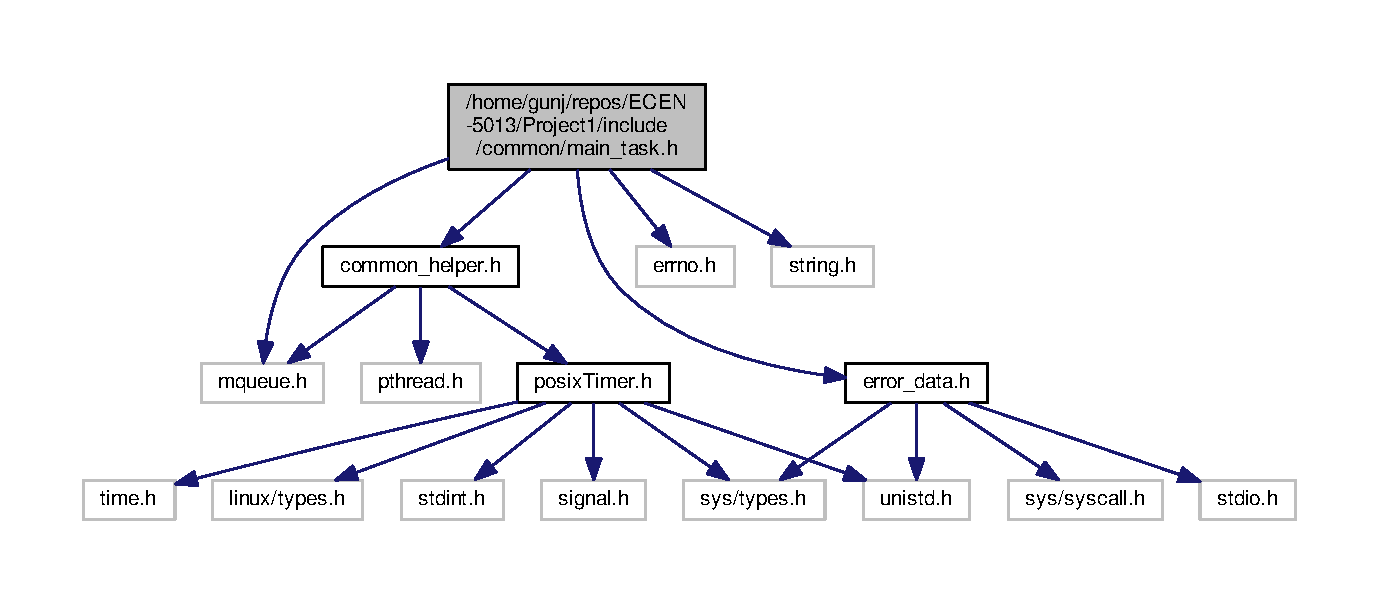
\includegraphics[width=350pt]{main__task_8h__incl}
\end{center}
\end{figure}
This graph shows which files directly or indirectly include this file\+:\nopagebreak
\begin{figure}[H]
\begin{center}
\leavevmode
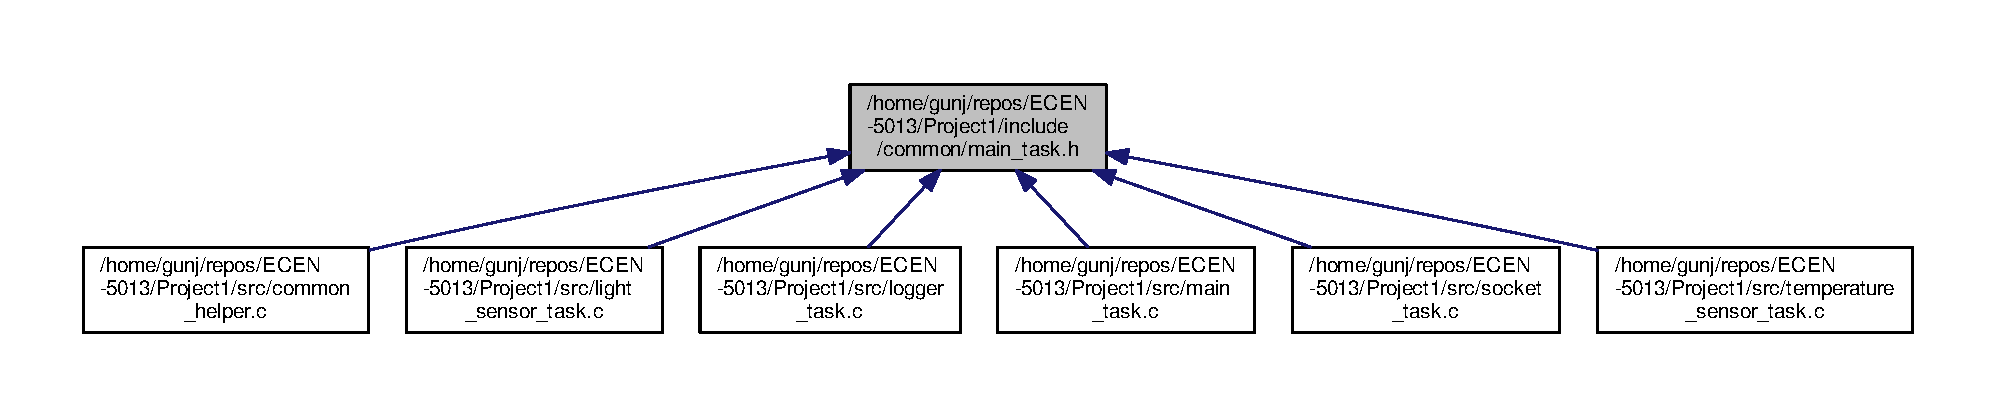
\includegraphics[width=350pt]{main__task_8h__dep__incl}
\end{center}
\end{figure}
\subsection*{Data Structures}
\begin{DoxyCompactItemize}
\item 
struct \hyperlink{structMAINTASKQ__MSG__T}{M\+A\+I\+N\+T\+A\+S\+K\+Q\+\_\+\+M\+S\+G\+\_\+T}
\end{DoxyCompactItemize}
\subsection*{Macros}
\begin{DoxyCompactItemize}
\item 
\#define {\bfseries M\+T\+\_\+\+M\+S\+G\+\_\+\+S\+I\+ZE}~20\hypertarget{main__task_8h_a2d4ecced2466e472574d62f82cc7da19}{}\label{main__task_8h_a2d4ecced2466e472574d62f82cc7da19}

\item 
\#define \hyperlink{main__task_8h_a457d4759d056b6c98f3966506d480eae}{D\+E\+F\+I\+N\+E\+\_\+\+M\+A\+I\+N\+T\+A\+S\+K\+\_\+\+S\+T\+R\+U\+CT}(name,  msg\+Id,  source\+Id)
\begin{DoxyCompactList}\small\item\em Defines a Main task queue struct with the name given and params with some default values. \end{DoxyCompactList}\item 
\#define {\bfseries P\+O\+S\+T\+\_\+\+M\+E\+S\+S\+A\+G\+E\+\_\+\+M\+A\+I\+N\+T\+A\+SK}(p\+\_\+maintaskstruct,  format, ...)
\end{DoxyCompactItemize}
\subsection*{Typedefs}
\begin{DoxyCompactItemize}
\item 
typedef char {\bfseries M\+A\+I\+N\+T\+\_\+\+T\+A\+S\+K\+\_\+\+M\+S\+G\+D\+A\+T\+A\+\_\+T}\hypertarget{main__task_8h_af70ff19e945c4a17b622920b428f3132}{}\label{main__task_8h_af70ff19e945c4a17b622920b428f3132}

\end{DoxyCompactItemize}
\subsection*{Enumerations}
\begin{DoxyCompactItemize}
\item 
enum {\bfseries M\+A\+I\+N\+T\+A\+S\+K\+Q\+\_\+\+M\+S\+G\+I\+D\+\_\+T} \{ {\bfseries M\+T\+\_\+\+M\+S\+G\+\_\+\+S\+T\+A\+T\+U\+S\+\_\+\+R\+SP}, 
{\bfseries M\+T\+\_\+\+M\+S\+G\+\_\+\+I\+N\+I\+T\+\_\+\+S\+U\+C\+C\+E\+S\+S\+\_\+\+R\+SP}
 \}\hypertarget{main__task_8h_ad5eb80ad0711fe40ab2f80bd98b11c20}{}\label{main__task_8h_ad5eb80ad0711fe40ab2f80bd98b11c20}

\end{DoxyCompactItemize}
\subsection*{Functions}
\begin{DoxyCompactItemize}
\item 
mqd\+\_\+t \hyperlink{main__task_8h_ad539583e28fb9162099dfd54fc34afc8}{get\+Handle\+\_\+\+Main\+Task\+Queue} ()
\begin{DoxyCompactList}\small\item\em Get the Handle Main\+Task\+Queue object. \end{DoxyCompactList}\item 
int \hyperlink{main__task_8h_a52c4c165f42a1ca113ba4bd55b00a293}{main\+\_\+task\+\_\+entry} ()
\begin{DoxyCompactList}\small\item\em entry point for the main task \end{DoxyCompactList}\end{DoxyCompactItemize}


\subsection{Detailed Description}
\begin{DoxyAuthor}{Author}
Gunj Manseta 
\end{DoxyAuthor}
\begin{DoxyDate}{Date}
2018-\/03-\/09 
\end{DoxyDate}


\subsection{Macro Definition Documentation}
\index{main\+\_\+task.\+h@{main\+\_\+task.\+h}!D\+E\+F\+I\+N\+E\+\_\+\+M\+A\+I\+N\+T\+A\+S\+K\+\_\+\+S\+T\+R\+U\+CT@{D\+E\+F\+I\+N\+E\+\_\+\+M\+A\+I\+N\+T\+A\+S\+K\+\_\+\+S\+T\+R\+U\+CT}}
\index{D\+E\+F\+I\+N\+E\+\_\+\+M\+A\+I\+N\+T\+A\+S\+K\+\_\+\+S\+T\+R\+U\+CT@{D\+E\+F\+I\+N\+E\+\_\+\+M\+A\+I\+N\+T\+A\+S\+K\+\_\+\+S\+T\+R\+U\+CT}!main\+\_\+task.\+h@{main\+\_\+task.\+h}}
\subsubsection[{\texorpdfstring{D\+E\+F\+I\+N\+E\+\_\+\+M\+A\+I\+N\+T\+A\+S\+K\+\_\+\+S\+T\+R\+U\+CT}{DEFINE_MAINTASK_STRUCT}}]{\setlength{\rightskip}{0pt plus 5cm}\#define D\+E\+F\+I\+N\+E\+\_\+\+M\+A\+I\+N\+T\+A\+S\+K\+\_\+\+S\+T\+R\+U\+CT(
\begin{DoxyParamCaption}
\item[{}]{name, }
\item[{}]{msg\+Id, }
\item[{}]{source\+Id}
\end{DoxyParamCaption}
)}\hypertarget{main__task_8h_a457d4759d056b6c98f3966506d480eae}{}\label{main__task_8h_a457d4759d056b6c98f3966506d480eae}
{\bfseries Value\+:}
\begin{DoxyCode}
\hyperlink{structMAINTASKQ__MSG__T}{MAINTASKQ\_MSG\_T} name = \{      \(\backslash\)
        .msgID      = msgId,        \(\backslash\)
        .sourceID   = sourceId,     \(\backslash\)
        .msgData    = \{0\}           \(\backslash\)
    \};
\end{DoxyCode}


Defines a Main task queue struct with the name given and params with some default values. 

\index{main\+\_\+task.\+h@{main\+\_\+task.\+h}!P\+O\+S\+T\+\_\+\+M\+E\+S\+S\+A\+G\+E\+\_\+\+M\+A\+I\+N\+T\+A\+SK@{P\+O\+S\+T\+\_\+\+M\+E\+S\+S\+A\+G\+E\+\_\+\+M\+A\+I\+N\+T\+A\+SK}}
\index{P\+O\+S\+T\+\_\+\+M\+E\+S\+S\+A\+G\+E\+\_\+\+M\+A\+I\+N\+T\+A\+SK@{P\+O\+S\+T\+\_\+\+M\+E\+S\+S\+A\+G\+E\+\_\+\+M\+A\+I\+N\+T\+A\+SK}!main\+\_\+task.\+h@{main\+\_\+task.\+h}}
\subsubsection[{\texorpdfstring{P\+O\+S\+T\+\_\+\+M\+E\+S\+S\+A\+G\+E\+\_\+\+M\+A\+I\+N\+T\+A\+SK}{POST_MESSAGE_MAINTASK}}]{\setlength{\rightskip}{0pt plus 5cm}\#define P\+O\+S\+T\+\_\+\+M\+E\+S\+S\+A\+G\+E\+\_\+\+M\+A\+I\+N\+T\+A\+SK(
\begin{DoxyParamCaption}
\item[{}]{p\+\_\+maintaskstruct, }
\item[{}]{format, }
\item[{}]{...}
\end{DoxyParamCaption}
)}\hypertarget{main__task_8h_ae94e2361e513b95ba8aae96361661425}{}\label{main__task_8h_ae94e2361e513b95ba8aae96361661425}
{\bfseries Value\+:}
\begin{DoxyCode}
\textcolor{keywordflow}{do}\{ \(\backslash\)
        snprintf((p\_maintaskstruct)->msgData,\textcolor{keyword}{sizeof}((p\_maintaskstruct)->msgData),format, ##\_\_VA\_ARGS\_\_);   
      \(\backslash\)
        \_\_POST\_MESSAGE\_MAINTASK(\hyperlink{main__task_8h_ad539583e28fb9162099dfd54fc34afc8}{getHandle\_MainTaskQueue}(), p\_maintaskstruct, \textcolor{keyword}{sizeof}(
      *p\_maintaskstruct)); \(\backslash\)
    \}\textcolor{keywordflow}{while}(0)
\end{DoxyCode}


\subsection{Function Documentation}
\index{main\+\_\+task.\+h@{main\+\_\+task.\+h}!get\+Handle\+\_\+\+Main\+Task\+Queue@{get\+Handle\+\_\+\+Main\+Task\+Queue}}
\index{get\+Handle\+\_\+\+Main\+Task\+Queue@{get\+Handle\+\_\+\+Main\+Task\+Queue}!main\+\_\+task.\+h@{main\+\_\+task.\+h}}
\subsubsection[{\texorpdfstring{get\+Handle\+\_\+\+Main\+Task\+Queue()}{getHandle_MainTaskQueue()}}]{\setlength{\rightskip}{0pt plus 5cm}mqd\+\_\+t get\+Handle\+\_\+\+Main\+Task\+Queue (
\begin{DoxyParamCaption}
{}
\end{DoxyParamCaption}
)}\hypertarget{main__task_8h_ad539583e28fb9162099dfd54fc34afc8}{}\label{main__task_8h_ad539583e28fb9162099dfd54fc34afc8}


Get the Handle Main\+Task\+Queue object. 

\begin{DoxyReturn}{Returns}
mqd\+\_\+t 
\end{DoxyReturn}

\begin{DoxyCode}
140 \{
141     \textcolor{keywordflow}{return} maintask\_q;
142 \}
\end{DoxyCode}
\index{main\+\_\+task.\+h@{main\+\_\+task.\+h}!main\+\_\+task\+\_\+entry@{main\+\_\+task\+\_\+entry}}
\index{main\+\_\+task\+\_\+entry@{main\+\_\+task\+\_\+entry}!main\+\_\+task.\+h@{main\+\_\+task.\+h}}
\subsubsection[{\texorpdfstring{main\+\_\+task\+\_\+entry()}{main_task_entry()}}]{\setlength{\rightskip}{0pt plus 5cm}int main\+\_\+task\+\_\+entry (
\begin{DoxyParamCaption}
{}
\end{DoxyParamCaption}
)}\hypertarget{main__task_8h_a52c4c165f42a1ca113ba4bd55b00a293}{}\label{main__task_8h_a52c4c165f42a1ca113ba4bd55b00a293}


entry point for the main task 

\begin{DoxyReturn}{Returns}
int 
\end{DoxyReturn}

\begin{DoxyCode}
211 \{
212     \textcolor{comment}{/* Making the timeout flag true, this should be unset=false within 5 sec else the timer checking the
       operation }
213 \textcolor{comment}{    will send a kill signal and the app will close}
214 \textcolor{comment}{    This is to make sure that the barrier is passed within 5 secs. Extra safety feature which might not be
       neccessary at all.}
215 \textcolor{comment}{    */}
216     timeoutflag = 1;
217     signal\_exit = 0;
218     \textcolor{keywordtype}{int} ret = main\_task\_init();    
219     \textcolor{keywordflow}{if}(-1 == ret)
220     \{
221         LOG\_STDOUT(ERROR \textcolor{stringliteral}{"MAIN TASK INIT:%s\(\backslash\)n"},strerror(errno));
222         \textcolor{keywordflow}{return} ret;
223     \}
224 
225     ret = \hyperlink{readConfiguration_8c_af04c65a7de574da1abe2b9bd0f403c64}{configdata\_setup}();
226     \textcolor{keywordflow}{if}(ret)
227         LOG\_STDOUT(ERROR \textcolor{stringliteral}{"Could not setup data from config file\(\backslash\)n"});
228 
229     \textcolor{comment}{/* Mutex init */}
230     pthread\_mutex\_init(&aliveState\_lock, NULL);
231 
232     \textcolor{comment}{/* Registering a timer for 5 sec to check that the barrier is passed */}
233     timer\_t timer\_id;
234     \textcolor{keywordflow}{if}(ERR == \hyperlink{common__helper_8c_a23124253b968391b9777fc3b8a0cc5ec}{register\_and\_start\_timer}(&timer\_id, 2*MICROSEC, 1, 
      timer\_handler\_setup, &timer\_id))
235     \{
236         \textcolor{comment}{// LOG\_STDOUT(ERROR "Timer Error\(\backslash\)n");}
237         \textcolor{keywordflow}{return} ERR;
238     \}
239 
240     \textcolor{comment}{/* Create a barrier for all the threads + the main task*/}
241     pthread\_barrier\_init(&tasks\_barrier,NULL,NUM\_CHILD\_THREADS+1);
242 
243     \textcolor{keyword}{struct }sigaction sa;
244     \textcolor{comment}{/*Registering the signal callback handler*/}
245     \hyperlink{my__signals_8c_ab23ded226351ef07fcd948a6d04a06e7}{register\_signalHandler}(&sa,signal\_handler, REG\_SIG\_ALL);
246 
247     \textcolor{comment}{/* Create all the child threads */}
248     \textcolor{keywordflow}{for}(\textcolor{keywordtype}{int} i = 0; i < NUM\_CHILD\_THREADS; i++)
249     \{
250         ret = pthread\_create(&pthread\_id[i],NULL,thread\_callbacks[i],NULL);
251         \textcolor{keywordflow}{if}(ret != 0)
252         \{
253             LOG\_STDOUT(ERROR \textcolor{stringliteral}{"Pthread create:%d:%s\(\backslash\)n"},i,strerror(errno));
254             \textcolor{keywordflow}{return} ret;
255         \}
256     \}
257 
258     LOG\_STDOUT(INFO \textcolor{stringliteral}{"MAIN TASK INIT COMPLETED\(\backslash\)n"});
259     pthread\_barrier\_wait(&tasks\_barrier);
260 
261     \textcolor{comment}{/* Resetting the timeoutflag as we are pass the barrier */}
262     timeoutflag = 0;
263 
264     ret= \hyperlink{posixTimer_8c_a33e0f810c8ecdcde8340650106da0958}{stop\_timer}(timer\_id);
265     \textcolor{keywordflow}{if}(ERR == ret)
266     \{
267         LOG\_STDOUT(ERROR \textcolor{stringliteral}{"MAIN TASK CANNOT STOP TIMER:%s\(\backslash\)n"},strerror(errno));
268         \textcolor{keywordflow}{return} ERR;
269     \}
270 
271     ret == \hyperlink{posixTimer_8c_a91f15230e46caba2a2132b04e9c73e47}{delete\_timer}(timer\_id);
272     \textcolor{keywordflow}{if}(ERR == ret)
273     \{
274         LOG\_STDOUT(ERROR \textcolor{stringliteral}{"MAIN TASK CANNOT DELETE TIMER:%s\(\backslash\)n"},strerror(errno));
275     \}
276 
277     \textcolor{keywordflow}{if}(ERR == \hyperlink{common__helper_8c_a23124253b968391b9777fc3b8a0cc5ec}{register\_and\_start\_timer}(&timer\_id, 5*MICROSEC, 0 ,
      timer\_handler\_aliveStatusCheck, &timer\_id))
278     \{
279         \textcolor{comment}{// LOG\_STDOUT(ERROR "Timer Start Error\(\backslash\)n");}
280         \textcolor{keywordflow}{return} ERR;
281     \}
282     \textcolor{comment}{/* Start message processing which is a blocking call */}
283     main\_task\_processMsg();
284 
285     \hyperlink{posixTimer_8c_a91f15230e46caba2a2132b04e9c73e47}{delete\_timer}(timer\_id);
286 
287     POST\_EXIT\_MESSAGE\_ALL();
288     
289     \textcolor{keywordflow}{for}(\textcolor{keywordtype}{int} i = 0; i < NUM\_CHILD\_THREADS; i++)
290     \{
291         \textcolor{keywordtype}{int} retThread = 0;
292         \textcolor{comment}{//  LOG\_STDOUT(INFO "Pthread JOIN:%d\(\backslash\)n",i);}
293         ret = pthread\_join(pthread\_id[i],(\textcolor{keywordtype}{void}*)&retThread);
294         \textcolor{comment}{//  LOG\_STDOUT(INFO "ThreadID %d: Ret:%d\(\backslash\)n",i,retThread);}
295         \textcolor{keywordflow}{if}(ret  != 0)
296         \{
297             LOG\_STDOUT(ERROR \textcolor{stringliteral}{"Pthread join:%d:%s\(\backslash\)n"},i,strerror(errno));
298             \textcolor{keywordflow}{return} ret;
299         \}
300     \}
301 
302     pthread\_mutex\_destroy(&aliveState\_lock);
303     
304     \hyperlink{readConfiguration_8c_a93341cc941d5255d844aea3b49cdfc9e}{configdata\_flush}();
305 
306     LOG\_STDOUT(INFO \textcolor{stringliteral}{"GOODBYE CRUEL WORLD!!!\(\backslash\)n"});
307 
308     \textcolor{keywordflow}{return} SUCCESS;
309 \}
\end{DoxyCode}

\hypertarget{my__signals_8h}{}\section{/home/gunj/repos/\+E\+C\+E\+N-\/5013/\+Project1/include/common/my\+\_\+signals.h File Reference}
\label{my__signals_8h}\index{/home/gunj/repos/\+E\+C\+E\+N-\/5013/\+Project1/include/common/my\+\_\+signals.\+h@{/home/gunj/repos/\+E\+C\+E\+N-\/5013/\+Project1/include/common/my\+\_\+signals.\+h}}
{\ttfamily \#include $<$sys/types.\+h$>$}\\*
{\ttfamily \#include $<$unistd.\+h$>$}\\*
{\ttfamily \#include $<$signal.\+h$>$}\\*
{\ttfamily \#include $<$stdint.\+h$>$}\\*
Include dependency graph for my\+\_\+signals.\+h\+:
\nopagebreak
\begin{figure}[H]
\begin{center}
\leavevmode
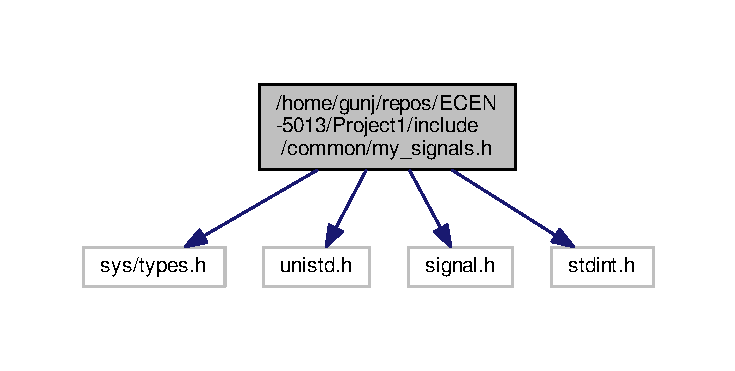
\includegraphics[width=350pt]{my__signals_8h__incl}
\end{center}
\end{figure}
This graph shows which files directly or indirectly include this file\+:
\nopagebreak
\begin{figure}[H]
\begin{center}
\leavevmode
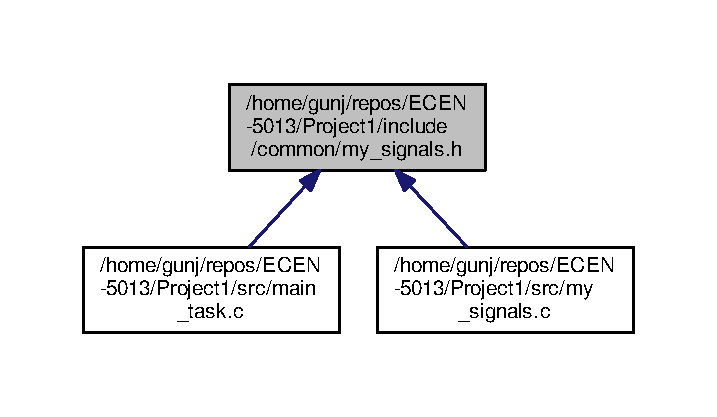
\includegraphics[width=344pt]{my__signals_8h__dep__incl}
\end{center}
\end{figure}
\subsection*{Macros}
\begin{DoxyCompactItemize}
\item 
\#define {\bfseries R\+E\+G\+\_\+\+S\+I\+G\+\_\+\+U\+S\+R1}~(1$<$$<$0)\hypertarget{my__signals_8h_a0e45ab7106dfdfab1129adbac64da0e6}{}\label{my__signals_8h_a0e45ab7106dfdfab1129adbac64da0e6}

\item 
\#define {\bfseries R\+E\+G\+\_\+\+S\+I\+G\+\_\+\+U\+S\+R2}~(1$<$$<$1)\hypertarget{my__signals_8h_a914eca0d337b1124ddb62fbafefac12b}{}\label{my__signals_8h_a914eca0d337b1124ddb62fbafefac12b}

\item 
\#define {\bfseries R\+E\+G\+\_\+\+S\+I\+G\+\_\+\+I\+NT}~(1$<$$<$2)\hypertarget{my__signals_8h_a2fca85c0a15f6e61404ace932ceca979}{}\label{my__signals_8h_a2fca85c0a15f6e61404ace932ceca979}

\item 
\#define {\bfseries R\+E\+G\+\_\+\+S\+I\+G\+\_\+\+T\+E\+RM}~(1$<$$<$3)\hypertarget{my__signals_8h_a7ed483de9d9805089ceb60d9d4c8bb2a}{}\label{my__signals_8h_a7ed483de9d9805089ceb60d9d4c8bb2a}

\item 
\#define {\bfseries R\+E\+G\+\_\+\+S\+I\+G\+\_\+\+T\+S\+TP}~(1$<$$<$4)\hypertarget{my__signals_8h_a1348f26f1d0b7c05aa713f8a13411ea9}{}\label{my__signals_8h_a1348f26f1d0b7c05aa713f8a13411ea9}

\item 
\#define {\bfseries R\+E\+G\+\_\+\+S\+I\+G\+\_\+\+A\+LL}~(0x1\+F)\hypertarget{my__signals_8h_a33370f69916d47556a24af7835b0bdad}{}\label{my__signals_8h_a33370f69916d47556a24af7835b0bdad}

\end{DoxyCompactItemize}
\subsection*{Typedefs}
\begin{DoxyCompactItemize}
\item 
typedef uint8\+\_\+t {\bfseries R\+E\+G\+\_\+\+S\+I\+G\+N\+A\+L\+\_\+\+F\+L\+A\+G\+\_\+t}\hypertarget{my__signals_8h_a5b58cc6fd2b95b7ca20155ad5936e1f0}{}\label{my__signals_8h_a5b58cc6fd2b95b7ca20155ad5936e1f0}

\end{DoxyCompactItemize}
\subsection*{Functions}
\begin{DoxyCompactItemize}
\item 
int \hyperlink{my__signals_8h_ab23ded226351ef07fcd948a6d04a06e7}{register\+\_\+signal\+Handler} (struct sigaction $\ast$sa, void($\ast$handler)(int), R\+E\+G\+\_\+\+S\+I\+G\+N\+A\+L\+\_\+\+F\+L\+A\+G\+\_\+t signal\+Mask)
\begin{DoxyCompactList}\small\item\em Register asignal handler for specific signal masks. \end{DoxyCompactList}\end{DoxyCompactItemize}


\subsection{Detailed Description}
\begin{DoxyAuthor}{Author}
Gunj Manseta 
\end{DoxyAuthor}
\begin{DoxyDate}{Date}
2018-\/03-\/18 
\end{DoxyDate}


\subsection{Function Documentation}
\index{my\+\_\+signals.\+h@{my\+\_\+signals.\+h}!register\+\_\+signal\+Handler@{register\+\_\+signal\+Handler}}
\index{register\+\_\+signal\+Handler@{register\+\_\+signal\+Handler}!my\+\_\+signals.\+h@{my\+\_\+signals.\+h}}
\subsubsection[{\texorpdfstring{register\+\_\+signal\+Handler(struct sigaction $\ast$sa, void($\ast$handler)(int), R\+E\+G\+\_\+\+S\+I\+G\+N\+A\+L\+\_\+\+F\+L\+A\+G\+\_\+t signal\+Mask)}{register_signalHandler(struct sigaction *sa, void(*handler)(int), REG_SIGNAL_FLAG_t signalMask)}}]{\setlength{\rightskip}{0pt plus 5cm}int register\+\_\+signal\+Handler (
\begin{DoxyParamCaption}
\item[{struct sigaction $\ast$}]{sa, }
\item[{void($\ast$)(int)}]{handler, }
\item[{R\+E\+G\+\_\+\+S\+I\+G\+N\+A\+L\+\_\+\+F\+L\+A\+G\+\_\+t}]{signal\+Mask}
\end{DoxyParamCaption}
)}\hypertarget{my__signals_8h_ab23ded226351ef07fcd948a6d04a06e7}{}\label{my__signals_8h_ab23ded226351ef07fcd948a6d04a06e7}


Register asignal handler for specific signal masks. 


\begin{DoxyParams}{Parameters}
{\em sa} & \\
\hline
{\em handler} & \\
\hline
{\em signal\+Mask} & \\
\hline
\end{DoxyParams}
\begin{DoxyReturn}{Returns}
int 
\end{DoxyReturn}

\begin{DoxyCode}
13 \{
14     sa->sa\_handler = handler;
15 
16     sa->sa\_flags = SA\_RESTART;
17 
18     sigfillset(&sa->sa\_mask);
19 
20     \textcolor{keywordtype}{int} ret\_error = 0;
21     
22     \textcolor{keywordflow}{if} ((signalMask & REG\_SIG\_USR1) && sigaction(SIGUSR1, sa, NULL) == -1) 
23     \{
24         ret\_error++;
25         LOG\_STDOUT(ERROR \textcolor{stringliteral}{"Cannot handle SIGUSR1.\(\backslash\)n"});
26     \}
27 
28     \textcolor{keywordflow}{if} ((signalMask & REG\_SIG\_USR2) && sigaction(SIGUSR2, sa, NULL) == -1) 
29     \{
30         ret\_error++;
31         LOG\_STDOUT(ERROR \textcolor{stringliteral}{"Cannot handle SIGUSR2.\(\backslash\)n"});
32     \}
33     
34     \textcolor{keywordflow}{if} ((signalMask & REG\_SIG\_INT) && sigaction(SIGINT, sa, NULL) == -1) 
35     \{
36         ret\_error++;
37         LOG\_STDOUT(ERROR \textcolor{stringliteral}{"Cannot handle SIGINT.\(\backslash\)n"});
38     \}
39     
40     \textcolor{keywordflow}{if} ((signalMask & REG\_SIG\_TSTP) && sigaction(SIGTERM, sa, NULL) == -1) 
41     \{
42         ret\_error++;
43         LOG\_STDOUT(ERROR \textcolor{stringliteral}{"Cannot handle SIGTERM.\(\backslash\)n"});
44     \}
45     
46     \textcolor{keywordflow}{if} ((signalMask & REG\_SIG\_TSTP) && sigaction(SIGTSTP, sa, NULL) == -1) 
47     \{
48         ret\_error++;
49         LOG\_STDOUT(ERROR \textcolor{stringliteral}{"Cannot handle SIGTSTOP.\(\backslash\)n"});
50     \}
51 
52     \textcolor{keywordflow}{return} ret\_error;
53 \}
\end{DoxyCode}


Here is the caller graph for this function\+:
\nopagebreak
\begin{figure}[H]
\begin{center}
\leavevmode
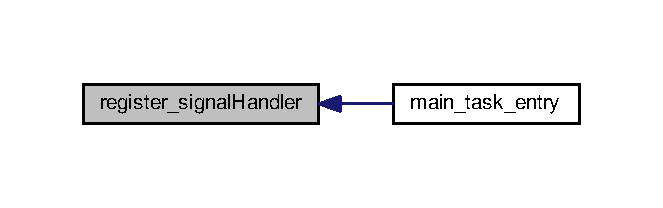
\includegraphics[width=318pt]{my__signals_8h_ab23ded226351ef07fcd948a6d04a06e7_icgraph}
\end{center}
\end{figure}



\hypertarget{my__time_8h}{}\section{/home/gunj/repos/\+E\+C\+E\+N-\/5013/\+Project1/include/common/my\+\_\+time.h File Reference}
\label{my__time_8h}\index{/home/gunj/repos/\+E\+C\+E\+N-\/5013/\+Project1/include/common/my\+\_\+time.\+h@{/home/gunj/repos/\+E\+C\+E\+N-\/5013/\+Project1/include/common/my\+\_\+time.\+h}}
This graph shows which files directly or indirectly include this file\+:\nopagebreak
\begin{figure}[H]
\begin{center}
\leavevmode
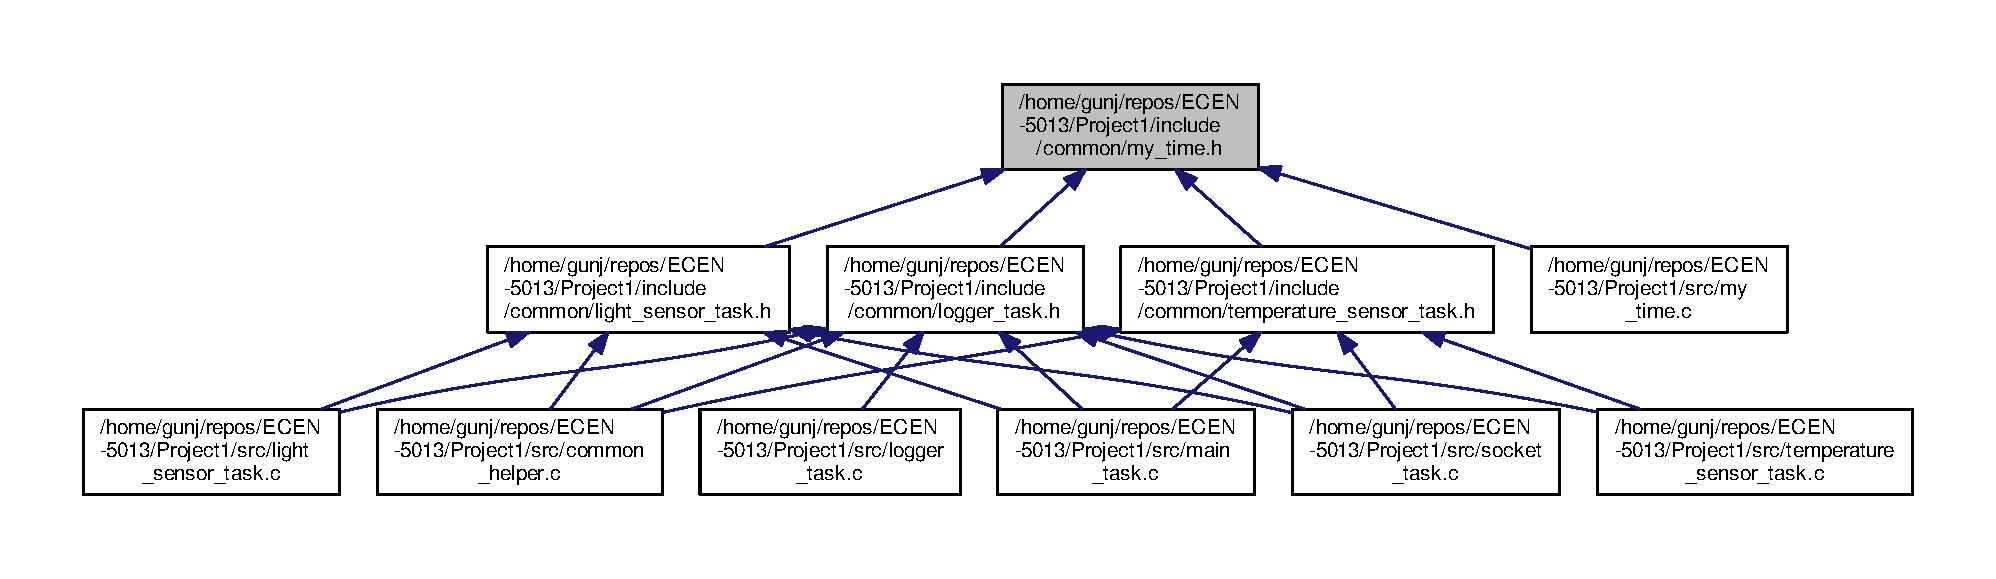
\includegraphics[width=350pt]{my__time_8h__dep__incl}
\end{center}
\end{figure}
\subsection*{Functions}
\begin{DoxyCompactItemize}
\item 
int \hyperlink{my__time_8h_a3385e59201decd0fae390437721a7d7e}{get\+\_\+time\+\_\+string} (char $\ast$time\+String, int len)
\begin{DoxyCompactList}\small\item\em Get the time string object. \end{DoxyCompactList}\end{DoxyCompactItemize}


\subsection{Detailed Description}
\begin{DoxyAuthor}{Author}
Gunj Manseta 
\end{DoxyAuthor}
\begin{DoxyDate}{Date}
2018-\/03-\/18 
\end{DoxyDate}


\subsection{Function Documentation}
\index{my\+\_\+time.\+h@{my\+\_\+time.\+h}!get\+\_\+time\+\_\+string@{get\+\_\+time\+\_\+string}}
\index{get\+\_\+time\+\_\+string@{get\+\_\+time\+\_\+string}!my\+\_\+time.\+h@{my\+\_\+time.\+h}}
\subsubsection[{\texorpdfstring{get\+\_\+time\+\_\+string(char $\ast$time\+String, int len)}{get_time_string(char *timeString, int len)}}]{\setlength{\rightskip}{0pt plus 5cm}int get\+\_\+time\+\_\+string (
\begin{DoxyParamCaption}
\item[{char $\ast$}]{time\+String, }
\item[{int}]{len}
\end{DoxyParamCaption}
)}\hypertarget{my__time_8h_a3385e59201decd0fae390437721a7d7e}{}\label{my__time_8h_a3385e59201decd0fae390437721a7d7e}


Get the time string object. 


\begin{DoxyParams}{Parameters}
{\em time\+String} & \\
\hline
{\em len} & \\
\hline
\end{DoxyParams}
\begin{DoxyReturn}{Returns}
int 
\end{DoxyReturn}

\begin{DoxyCode}
18 \{
19     \textcolor{keyword}{struct }timeval tv;
20     \textcolor{comment}{//struct tm* ptm;}
21     \textcolor{keywordtype}{char} time\_string[20] = \{0\};
22 
23     \textcolor{comment}{/* Obtain the time of day using the system call */}
24     \textcolor{keywordtype}{unsigned} \textcolor{keywordtype}{long} ret = GET\_TIMEOFDAY(&tv,NULL);
25     \textcolor{keywordflow}{if}(ret != 0)
26     \{
27         memset(timeString,0,len);
28         \textcolor{keywordflow}{return} ERR;
29     \}
30     snprintf(time\_string,\textcolor{keyword}{sizeof}(time\_string),\textcolor{stringliteral}{"%ld.%ld"},tv.tv\_sec,tv.tv\_usec);
31     \textcolor{comment}{//ptm = localtime (&tv.tv\_sec);}
32     \textcolor{comment}{/* Format the date and time. */}
33     \textcolor{comment}{//strftime (time\_string, sizeof (time\_string), "%Y-%m-%d %H:%M:%S", ptm);}
34     \textcolor{comment}{//strftime (time\_string, sizeof (time\_string), "%X", ptm);}
35     memcpy(timeString,time\_string, len);
36     
37     \textcolor{keywordflow}{return} SUCCESS;
38 \}
\end{DoxyCode}

\hypertarget{posixTimer_8h}{}\section{/home/gunj/repos/\+E\+C\+E\+N-\/5013/\+Project1/include/common/posix\+Timer.h File Reference}
\label{posixTimer_8h}\index{/home/gunj/repos/\+E\+C\+E\+N-\/5013/\+Project1/include/common/posix\+Timer.\+h@{/home/gunj/repos/\+E\+C\+E\+N-\/5013/\+Project1/include/common/posix\+Timer.\+h}}
{\ttfamily \#include $<$time.\+h$>$}\\*
{\ttfamily \#include $<$linux/types.\+h$>$}\\*
{\ttfamily \#include $<$stdint.\+h$>$}\\*
{\ttfamily \#include $<$sys/types.\+h$>$}\\*
{\ttfamily \#include $<$unistd.\+h$>$}\\*
{\ttfamily \#include $<$signal.\+h$>$}\\*
Include dependency graph for posix\+Timer.\+h\+:\nopagebreak
\begin{figure}[H]
\begin{center}
\leavevmode
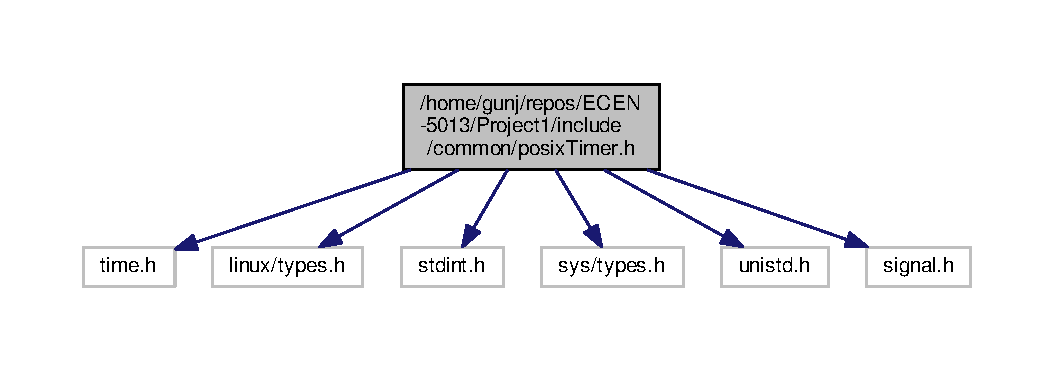
\includegraphics[width=350pt]{posixTimer_8h__incl}
\end{center}
\end{figure}
This graph shows which files directly or indirectly include this file\+:\nopagebreak
\begin{figure}[H]
\begin{center}
\leavevmode
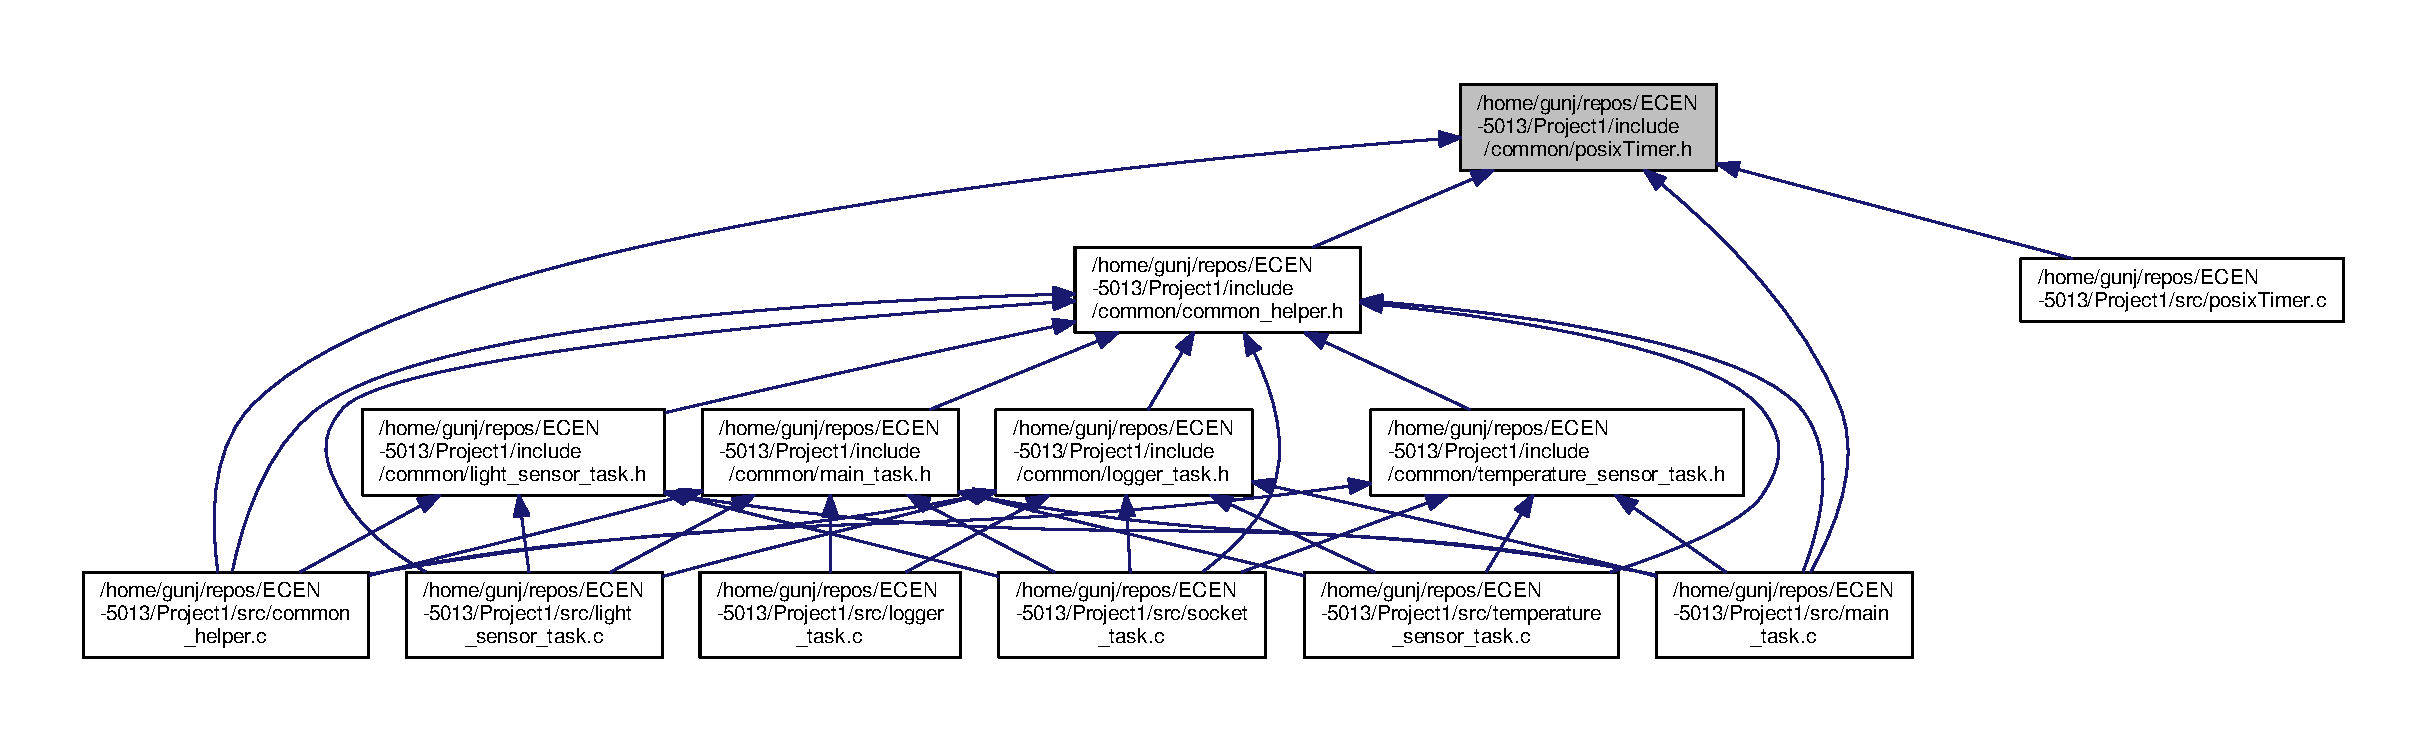
\includegraphics[width=350pt]{posixTimer_8h__dep__incl}
\end{center}
\end{figure}
\subsection*{Macros}
\begin{DoxyCompactItemize}
\item 
\#define {\bfseries M\+I\+C\+R\+O\+S\+EC}~(1000000)\hypertarget{posixTimer_8h_a3401c320bd609c5464b2eecb205321f9}{}\label{posixTimer_8h_a3401c320bd609c5464b2eecb205321f9}

\end{DoxyCompactItemize}
\subsection*{Functions}
\begin{DoxyCompactItemize}
\item 
int \hyperlink{posixTimer_8h_a731c8c8f52f8feb4c14fb91b0274d94f}{register\+\_\+timer} (timer\+\_\+t $\ast$timer\+\_\+id, void($\ast$timer\+\_\+handler)(union sigval), void $\ast$handler\+Args)
\begin{DoxyCompactList}\small\item\em R\+Egsiter the timer handler. \end{DoxyCompactList}\item 
int \hyperlink{posixTimer_8h_a659e3544e54a6fb4aeed6c38f4a91ad2}{start\+\_\+timer} (timer\+\_\+t timer\+\_\+id, uint64\+\_\+t time\+\_\+usec, uint8\+\_\+t oneshot)
\begin{DoxyCompactList}\small\item\em Starts the timer. \end{DoxyCompactList}\item 
int \hyperlink{posixTimer_8h_a33e0f810c8ecdcde8340650106da0958}{stop\+\_\+timer} (timer\+\_\+t timer\+\_\+id)
\begin{DoxyCompactList}\small\item\em Stops the timer. \end{DoxyCompactList}\item 
int \hyperlink{posixTimer_8h_a91f15230e46caba2a2132b04e9c73e47}{delete\+\_\+timer} (timer\+\_\+t timer\+\_\+id)
\begin{DoxyCompactList}\small\item\em Destroys the timer. \end{DoxyCompactList}\end{DoxyCompactItemize}


\subsection{Detailed Description}
\begin{DoxyAuthor}{Author}
Gunj Manseta 
\end{DoxyAuthor}
\begin{DoxyDate}{Date}
2018-\/03-\/18 
\end{DoxyDate}


\subsection{Function Documentation}
\index{posix\+Timer.\+h@{posix\+Timer.\+h}!delete\+\_\+timer@{delete\+\_\+timer}}
\index{delete\+\_\+timer@{delete\+\_\+timer}!posix\+Timer.\+h@{posix\+Timer.\+h}}
\subsubsection[{\texorpdfstring{delete\+\_\+timer(timer\+\_\+t timer\+\_\+id)}{delete_timer(timer_t timer_id)}}]{\setlength{\rightskip}{0pt plus 5cm}int delete\+\_\+timer (
\begin{DoxyParamCaption}
\item[{timer\+\_\+t}]{timer\+\_\+id}
\end{DoxyParamCaption}
)}\hypertarget{posixTimer_8h_a91f15230e46caba2a2132b04e9c73e47}{}\label{posixTimer_8h_a91f15230e46caba2a2132b04e9c73e47}


Destroys the timer. 


\begin{DoxyParams}{Parameters}
{\em timer\+\_\+id} & \\
\hline
\end{DoxyParams}
\begin{DoxyReturn}{Returns}
int 
\end{DoxyReturn}

\begin{DoxyCode}
83 \{
84     \textcolor{comment}{// if(NULL == timer\_id)}
85     \textcolor{comment}{//  return -1;}
86     
87     \textcolor{keywordtype}{int} ret = timer\_delete(timer\_id);
88 
89     \textcolor{keywordflow}{return} ret;
90 
91 
92 \}
\end{DoxyCode}


Here is the caller graph for this function\+:\nopagebreak
\begin{figure}[H]
\begin{center}
\leavevmode
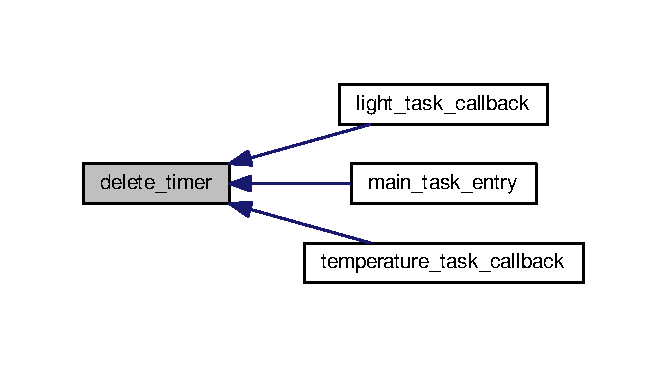
\includegraphics[width=320pt]{posixTimer_8h_a91f15230e46caba2a2132b04e9c73e47_icgraph}
\end{center}
\end{figure}


\index{posix\+Timer.\+h@{posix\+Timer.\+h}!register\+\_\+timer@{register\+\_\+timer}}
\index{register\+\_\+timer@{register\+\_\+timer}!posix\+Timer.\+h@{posix\+Timer.\+h}}
\subsubsection[{\texorpdfstring{register\+\_\+timer(timer\+\_\+t $\ast$timer\+\_\+id, void($\ast$timer\+\_\+handler)(union sigval), void $\ast$handler\+Args)}{register_timer(timer_t *timer_id, void(*timer_handler)(union sigval), void *handlerArgs)}}]{\setlength{\rightskip}{0pt plus 5cm}int register\+\_\+timer (
\begin{DoxyParamCaption}
\item[{timer\+\_\+t $\ast$}]{timer\+\_\+id, }
\item[{void($\ast$)(union sigval)}]{timer\+\_\+handler, }
\item[{void $\ast$}]{handler\+Args}
\end{DoxyParamCaption}
)}\hypertarget{posixTimer_8h_a731c8c8f52f8feb4c14fb91b0274d94f}{}\label{posixTimer_8h_a731c8c8f52f8feb4c14fb91b0274d94f}


R\+Egsiter the timer handler. 


\begin{DoxyParams}{Parameters}
{\em timer\+\_\+id} & \\
\hline
{\em timer\+\_\+handler} & \\
\hline
{\em handler\+Args} & \\
\hline
\end{DoxyParams}
\begin{DoxyReturn}{Returns}
int 
\end{DoxyReturn}

\begin{DoxyCode}
20 \{
21 
22     \textcolor{keywordflow}{if}(NULL == timer\_id)
23         \textcolor{keywordflow}{return} -1;
24         
25     \textcolor{keyword}{struct }sigevent sige;
26 
27     \textcolor{comment}{/*SIGEV\_THREAD will call the handler as if it was a new thread */}
28     sige.sigev\_notify = SIGEV\_THREAD;
29     sige.sigev\_notify\_function = timer\_handler;
30 \textcolor{comment}{//  sige.sigev\_value.sival\_ptr = timer\_id;}
31     sige.sigev\_value.sival\_ptr = handlerArgs;
32     sige.sigev\_notify\_attributes = NULL;
33 
34     \textcolor{keywordtype}{int} ret = timer\_create(CLOCK\_REALTIME, &sige, timer\_id);
35     
36     \textcolor{keywordflow}{return} ret;
37 \}
\end{DoxyCode}


Here is the caller graph for this function\+:\nopagebreak
\begin{figure}[H]
\begin{center}
\leavevmode
\includegraphics[width=350pt]{posixTimer_8h_a731c8c8f52f8feb4c14fb91b0274d94f_icgraph}
\end{center}
\end{figure}


\index{posix\+Timer.\+h@{posix\+Timer.\+h}!start\+\_\+timer@{start\+\_\+timer}}
\index{start\+\_\+timer@{start\+\_\+timer}!posix\+Timer.\+h@{posix\+Timer.\+h}}
\subsubsection[{\texorpdfstring{start\+\_\+timer(timer\+\_\+t timer\+\_\+id, uint64\+\_\+t time\+\_\+usec, uint8\+\_\+t oneshot)}{start_timer(timer_t timer_id, uint64_t time_usec, uint8_t oneshot)}}]{\setlength{\rightskip}{0pt plus 5cm}int start\+\_\+timer (
\begin{DoxyParamCaption}
\item[{timer\+\_\+t}]{timer\+\_\+id, }
\item[{uint64\+\_\+t}]{time\+\_\+usec, }
\item[{uint8\+\_\+t}]{oneshot}
\end{DoxyParamCaption}
)}\hypertarget{posixTimer_8h_a659e3544e54a6fb4aeed6c38f4a91ad2}{}\label{posixTimer_8h_a659e3544e54a6fb4aeed6c38f4a91ad2}


Starts the timer. 


\begin{DoxyParams}{Parameters}
{\em timer\+\_\+id} & \\
\hline
{\em time\+\_\+usec} & \\
\hline
{\em oneshot} & \\
\hline
\end{DoxyParams}
\begin{DoxyReturn}{Returns}
int 
\end{DoxyReturn}

\begin{DoxyCode}
40 \{
41     \textcolor{comment}{// if(NULL == timer\_id)}
42     \textcolor{comment}{//  return -1;}
43         
44     \textcolor{keyword}{struct }itimerspec ts;
45     
46     ts.it\_value.tv\_sec = time\_usec / MICROSEC;
47     ts.it\_value.tv\_nsec = (time\_usec % MICROSEC) * 1000;
48     \textcolor{keywordflow}{if}(1 == oneshot)
49     \{
50         ts.it\_interval.tv\_sec = 0;
51         ts.it\_interval.tv\_nsec = 0;
52     \}
53     \textcolor{keywordflow}{else}
54     \{
55         ts.it\_interval.tv\_sec = ts.it\_value.tv\_sec;
56         ts.it\_interval.tv\_nsec = ts.it\_value.tv\_nsec;
57     \}
58 
59     \textcolor{keywordtype}{int} ret = timer\_settime(timer\_id, 0, &ts, 0);
60     
61     \textcolor{keywordflow}{return} ret;
62 \}
\end{DoxyCode}


Here is the caller graph for this function\+:\nopagebreak
\begin{figure}[H]
\begin{center}
\leavevmode
\includegraphics[width=350pt]{posixTimer_8h_a659e3544e54a6fb4aeed6c38f4a91ad2_icgraph}
\end{center}
\end{figure}


\index{posix\+Timer.\+h@{posix\+Timer.\+h}!stop\+\_\+timer@{stop\+\_\+timer}}
\index{stop\+\_\+timer@{stop\+\_\+timer}!posix\+Timer.\+h@{posix\+Timer.\+h}}
\subsubsection[{\texorpdfstring{stop\+\_\+timer(timer\+\_\+t timer\+\_\+id)}{stop_timer(timer_t timer_id)}}]{\setlength{\rightskip}{0pt plus 5cm}int stop\+\_\+timer (
\begin{DoxyParamCaption}
\item[{timer\+\_\+t}]{timer\+\_\+id}
\end{DoxyParamCaption}
)}\hypertarget{posixTimer_8h_a33e0f810c8ecdcde8340650106da0958}{}\label{posixTimer_8h_a33e0f810c8ecdcde8340650106da0958}


Stops the timer. 


\begin{DoxyParams}{Parameters}
{\em timer\+\_\+id} & \\
\hline
\end{DoxyParams}
\begin{DoxyReturn}{Returns}
int 
\end{DoxyReturn}

\begin{DoxyCode}
65 \{
66     \textcolor{comment}{// if(NULL == timer\_id)}
67     \textcolor{comment}{//  return -1;}
68         
69     \textcolor{keyword}{struct }itimerspec ts;
70     
71     ts.it\_value.tv\_sec = 0;
72     ts.it\_value.tv\_nsec = 0;
73     ts.it\_interval.tv\_sec = 0;
74     ts.it\_interval.tv\_nsec = 0;
75 
76     \textcolor{keywordtype}{int} ret = timer\_settime(timer\_id, 0, &ts, 0);
77     
78     \textcolor{keywordflow}{return} ret;
79 \}
\end{DoxyCode}


Here is the caller graph for this function\+:\nopagebreak
\begin{figure}[H]
\begin{center}
\leavevmode
\includegraphics[width=267pt]{posixTimer_8h_a33e0f810c8ecdcde8340650106da0958_icgraph}
\end{center}
\end{figure}



\hypertarget{readConfiguration_8h}{}\section{/home/gunj/repos/\+E\+C\+E\+N-\/5013/\+Project1/include/common/read\+Configuration.h File Reference}
\label{readConfiguration_8h}\index{/home/gunj/repos/\+E\+C\+E\+N-\/5013/\+Project1/include/common/read\+Configuration.\+h@{/home/gunj/repos/\+E\+C\+E\+N-\/5013/\+Project1/include/common/read\+Configuration.\+h}}
This graph shows which files directly or indirectly include this file\+:\nopagebreak
\begin{figure}[H]
\begin{center}
\leavevmode
\includegraphics[width=350pt]{readConfiguration_8h__dep__incl}
\end{center}
\end{figure}
\subsection*{Functions}
\begin{DoxyCompactItemize}
\item 
char $\ast$ \hyperlink{readConfiguration_8h_a6ec4251859d1107c4a9f457ff5ead99c}{configdata\+\_\+get\+Logpath} ()
\item 
uint32\+\_\+t \hyperlink{readConfiguration_8h_a622fe97941be32a0343567a4cfbd24e7}{configdata\+\_\+get\+Setup\+Time} ()
\item 
uint32\+\_\+t \hyperlink{readConfiguration_8h_a3936001fcb10cb50f534070c1e0d3058}{configdata\+\_\+get\+Alive\+Timeout} ()
\item 
int \hyperlink{readConfiguration_8h_af04c65a7de574da1abe2b9bd0f403c64}{configdata\+\_\+setup} ()
\begin{DoxyCompactList}\small\item\em Should be called in the main task at the beginning. \end{DoxyCompactList}\item 
void \hyperlink{readConfiguration_8h_a93341cc941d5255d844aea3b49cdfc9e}{configdata\+\_\+flush} ()\hypertarget{readConfiguration_8h_a93341cc941d5255d844aea3b49cdfc9e}{}\label{readConfiguration_8h_a93341cc941d5255d844aea3b49cdfc9e}

\begin{DoxyCompactList}\small\item\em Should be called at teh end of main task. If not called, memory leak will occur. \end{DoxyCompactList}\end{DoxyCompactItemize}


\subsection{Detailed Description}
\begin{DoxyAuthor}{Author}
Gunj Manseta 
\end{DoxyAuthor}
\begin{DoxyDate}{Date}
2018-\/03-\/17 
\end{DoxyDate}


\subsection{Function Documentation}
\index{read\+Configuration.\+h@{read\+Configuration.\+h}!configdata\+\_\+get\+Alive\+Timeout@{configdata\+\_\+get\+Alive\+Timeout}}
\index{configdata\+\_\+get\+Alive\+Timeout@{configdata\+\_\+get\+Alive\+Timeout}!read\+Configuration.\+h@{read\+Configuration.\+h}}
\subsubsection[{\texorpdfstring{configdata\+\_\+get\+Alive\+Timeout()}{configdata_getAliveTimeout()}}]{\setlength{\rightskip}{0pt plus 5cm}uint32\+\_\+t configdata\+\_\+get\+Alive\+Timeout (
\begin{DoxyParamCaption}
{}
\end{DoxyParamCaption}
)}\hypertarget{readConfiguration_8h_a3936001fcb10cb50f534070c1e0d3058}{}\label{readConfiguration_8h_a3936001fcb10cb50f534070c1e0d3058}
\begin{DoxyReturn}{Returns}
uint32\+\_\+t 
\end{DoxyReturn}

\begin{DoxyCode}
40 \{
41     \textcolor{keywordflow}{return} (*((uint32\_t*)configurationData[TASK\_ALIVE\_TIMEOUT\_SEC\_UINT8]));
42 \}
\end{DoxyCode}


Here is the caller graph for this function\+:\nopagebreak
\begin{figure}[H]
\begin{center}
\leavevmode
\includegraphics[width=350pt]{readConfiguration_8h_a3936001fcb10cb50f534070c1e0d3058_icgraph}
\end{center}
\end{figure}


\index{read\+Configuration.\+h@{read\+Configuration.\+h}!configdata\+\_\+get\+Logpath@{configdata\+\_\+get\+Logpath}}
\index{configdata\+\_\+get\+Logpath@{configdata\+\_\+get\+Logpath}!read\+Configuration.\+h@{read\+Configuration.\+h}}
\subsubsection[{\texorpdfstring{configdata\+\_\+get\+Logpath()}{configdata_getLogpath()}}]{\setlength{\rightskip}{0pt plus 5cm}char$\ast$ configdata\+\_\+get\+Logpath (
\begin{DoxyParamCaption}
{}
\end{DoxyParamCaption}
)}\hypertarget{readConfiguration_8h_a6ec4251859d1107c4a9f457ff5ead99c}{}\label{readConfiguration_8h_a6ec4251859d1107c4a9f457ff5ead99c}
\begin{DoxyReturn}{Returns}
char$\ast$ 
\end{DoxyReturn}

\begin{DoxyCode}
31 \{
32     \textcolor{keywordflow}{return} ((\textcolor{keywordtype}{char}*)configurationData[LOG\_PATH\_STRING]);
33 \}
\end{DoxyCode}


Here is the caller graph for this function\+:\nopagebreak
\begin{figure}[H]
\begin{center}
\leavevmode
\includegraphics[width=350pt]{readConfiguration_8h_a6ec4251859d1107c4a9f457ff5ead99c_icgraph}
\end{center}
\end{figure}


\index{read\+Configuration.\+h@{read\+Configuration.\+h}!configdata\+\_\+get\+Setup\+Time@{configdata\+\_\+get\+Setup\+Time}}
\index{configdata\+\_\+get\+Setup\+Time@{configdata\+\_\+get\+Setup\+Time}!read\+Configuration.\+h@{read\+Configuration.\+h}}
\subsubsection[{\texorpdfstring{configdata\+\_\+get\+Setup\+Time()}{configdata_getSetupTime()}}]{\setlength{\rightskip}{0pt plus 5cm}uint32\+\_\+t configdata\+\_\+get\+Setup\+Time (
\begin{DoxyParamCaption}
{}
\end{DoxyParamCaption}
)}\hypertarget{readConfiguration_8h_a622fe97941be32a0343567a4cfbd24e7}{}\label{readConfiguration_8h_a622fe97941be32a0343567a4cfbd24e7}
\begin{DoxyReturn}{Returns}
uint32\+\_\+t 
\end{DoxyReturn}

\begin{DoxyCode}
36 \{
37     \textcolor{keywordflow}{return} (*((uint32\_t*)configurationData[TASK\_SETUP\_TIME\_SEC\_UINT8]));
38 \}
\end{DoxyCode}


Here is the caller graph for this function\+:\nopagebreak
\begin{figure}[H]
\begin{center}
\leavevmode
\includegraphics[width=350pt]{readConfiguration_8h_a622fe97941be32a0343567a4cfbd24e7_icgraph}
\end{center}
\end{figure}


\index{read\+Configuration.\+h@{read\+Configuration.\+h}!configdata\+\_\+setup@{configdata\+\_\+setup}}
\index{configdata\+\_\+setup@{configdata\+\_\+setup}!read\+Configuration.\+h@{read\+Configuration.\+h}}
\subsubsection[{\texorpdfstring{configdata\+\_\+setup()}{configdata_setup()}}]{\setlength{\rightskip}{0pt plus 5cm}int configdata\+\_\+setup (
\begin{DoxyParamCaption}
{}
\end{DoxyParamCaption}
)}\hypertarget{readConfiguration_8h_af04c65a7de574da1abe2b9bd0f403c64}{}\label{readConfiguration_8h_af04c65a7de574da1abe2b9bd0f403c64}


Should be called in the main task at the beginning. 

\begin{DoxyReturn}{Returns}
int 
\end{DoxyReturn}

\begin{DoxyCode}
45 \{
46     FILE *fp;
47     fp = fopen(CONFIG\_FILE, \textcolor{stringliteral}{"r"});
48     \textcolor{keywordflow}{if}(NULL ==fp)
49         \textcolor{keywordflow}{return} -1;
50     
51     configurationData[LOG\_PATH\_STRING] = (\textcolor{keywordtype}{char}*)malloc(\textcolor{keyword}{sizeof}(\textcolor{keywordtype}{char})*20);
52     configurationData[TASK\_SETUP\_TIME\_SEC\_UINT8] = (uint32\_t*)malloc(\textcolor{keyword}{sizeof}(uint32\_t));
53     configurationData[TASK\_ALIVE\_TIMEOUT\_SEC\_UINT8] = (uint32\_t*)malloc(\textcolor{keyword}{sizeof}(uint32\_t));
54 
55     \textcolor{keywordtype}{size\_t} readBytes = fscanf(fp,\textcolor{stringliteral}{"%s %u %u"},(\textcolor{keywordtype}{char}*)configurationData[LOG\_PATH\_STRING],(uint32\_t*)
      configurationData[TASK\_SETUP\_TIME\_SEC\_UINT8], (uint32\_t*)configurationData[TASK\_ALIVE\_TIMEOUT\_SEC\_UINT8]);
56     
57 \textcolor{preprocessor}{    #ifdef SELF\_TEST}
58     printf(\textcolor{stringliteral}{"PATH: %s\(\backslash\)n"},(\textcolor{keywordtype}{char}*)configurationData[LOG\_PATH\_STRING]);
59     printf(\textcolor{stringliteral}{"SETUP: %u\(\backslash\)n"},*(uint32\_t*)configurationData[TASK\_SETUP\_TIME\_SEC\_UINT8]);
60     printf(\textcolor{stringliteral}{"TO: %u\(\backslash\)n"},*(uint32\_t*)configurationData[TASK\_ALIVE\_TIMEOUT\_SEC\_UINT8]);
61 \textcolor{preprocessor}{    #endif}
62 
63     \textcolor{keywordflow}{return} 0;
64 \}
\end{DoxyCode}


Here is the caller graph for this function\+:\nopagebreak
\begin{figure}[H]
\begin{center}
\leavevmode
\includegraphics[width=350pt]{readConfiguration_8h_af04c65a7de574da1abe2b9bd0f403c64_icgraph}
\end{center}
\end{figure}



\hypertarget{sensor__common__object_8h}{}\section{/home/gunj/repos/\+E\+C\+E\+N-\/5013/\+Project1/include/common/sensor\+\_\+common\+\_\+object.h File Reference}
\label{sensor__common__object_8h}\index{/home/gunj/repos/\+E\+C\+E\+N-\/5013/\+Project1/include/common/sensor\+\_\+common\+\_\+object.\+h@{/home/gunj/repos/\+E\+C\+E\+N-\/5013/\+Project1/include/common/sensor\+\_\+common\+\_\+object.\+h}}
{\ttfamily \#include $<$stdint.\+h$>$}\\*
{\ttfamily \#include $<$semaphore.\+h$>$}\\*
Include dependency graph for sensor\+\_\+common\+\_\+object.\+h\+:
\nopagebreak
\begin{figure}[H]
\begin{center}
\leavevmode
\includegraphics[width=252pt]{sensor__common__object_8h__incl}
\end{center}
\end{figure}
This graph shows which files directly or indirectly include this file\+:
\nopagebreak
\begin{figure}[H]
\begin{center}
\leavevmode
\includegraphics[width=350pt]{sensor__common__object_8h__dep__incl}
\end{center}
\end{figure}
\subsection*{Data Structures}
\begin{DoxyCompactItemize}
\item 
struct \hyperlink{structREMOTE__REQUEST__T}{R\+E\+M\+O\+T\+E\+\_\+\+R\+E\+Q\+U\+E\+S\+T\+\_\+T}
\item 
struct \hyperlink{structREMOTE__RESPONSE__T}{R\+E\+M\+O\+T\+E\+\_\+\+R\+E\+S\+P\+O\+N\+S\+E\+\_\+T}
\item 
union \hyperlink{unionREMOTE__RESPONSE__T_1_1data}{R\+E\+M\+O\+T\+E\+\_\+\+R\+E\+S\+P\+O\+N\+S\+E\+\_\+\+T\+::data}
\item 
struct \hyperlink{structOBJECT__PACKET__T}{O\+B\+J\+E\+C\+T\+\_\+\+P\+A\+C\+K\+E\+T\+\_\+T}
\end{DoxyCompactItemize}
\subsection*{Macros}
\begin{DoxyCompactItemize}
\item 
\#define {\bfseries S\+E\+N\+S\+O\+R\+\_\+\+M\+A\+K\+E\+\_\+\+P\+A\+C\+K\+E\+T\+\_\+\+S\+Y\+N\+C\+T\+Y\+PE}(p\+\_\+packet,  p\+\_\+sem)~\{ p\+\_\+packet-\/$>$is\+\_\+sync = S\+Y\+NC; if(N\+U\+LL != p\+\_\+sem)\{p\+\_\+packet-\/$>$sync\+\_\+semaphore = p\+\_\+sem;\} \}\hypertarget{sensor__common__object_8h_aeb154e5d881c17aa08840aa0c0970e08}{}\label{sensor__common__object_8h_aeb154e5d881c17aa08840aa0c0970e08}

\item 
\#define {\bfseries S\+E\+N\+S\+O\+R\+\_\+\+M\+A\+K\+E\+\_\+\+P\+A\+C\+K\+E\+T\+\_\+\+A\+S\+Y\+N\+C\+T\+Y\+PE}(p\+\_\+packet)~\{p\+\_\+packet-\/$>$is\+\_\+sync = A\+S\+Y\+NC; p\+\_\+packet-\/$>$sync\+\_\+semaphore = N\+U\+LL;\}\hypertarget{sensor__common__object_8h_a0e5ecbc8009d353b51513dcdd4baaac7}{}\label{sensor__common__object_8h_a0e5ecbc8009d353b51513dcdd4baaac7}

\item 
\#define {\bfseries S\+E\+N\+S\+O\+R\+\_\+\+M\+A\+K\+E\+\_\+\+P\+A\+C\+K\+E\+T\+\_\+\+R\+W\+\_\+1\+D\+A\+TA}(p\+\_\+packet)~(p\+\_\+packet-\/$>$buff\+Len = 1)\hypertarget{sensor__common__object_8h_afb65c7303d7a4e2807ec1d27f3999007}{}\label{sensor__common__object_8h_afb65c7303d7a4e2807ec1d27f3999007}

\item 
\#define {\bfseries S\+E\+N\+S\+O\+R\+\_\+\+M\+A\+K\+E\+\_\+\+P\+A\+C\+K\+E\+T\+\_\+\+R\+W\+\_\+2\+D\+A\+TA}(p\+\_\+packet)~(p\+\_\+packet-\/$>$buff\+Len = 2)\hypertarget{sensor__common__object_8h_a1af2cf70b7bf90d76723e6f7d00fb3aa}{}\label{sensor__common__object_8h_a1af2cf70b7bf90d76723e6f7d00fb3aa}

\end{DoxyCompactItemize}
\subsection*{Typedefs}
\begin{DoxyCompactItemize}
\item 
typedef uint8\+\_\+t $\ast$ {\bfseries P\+\_\+\+B\+U\+F\+F\+\_\+T}\hypertarget{sensor__common__object_8h_aad357c71e0a9fbea0c6f670e8d0df991}{}\label{sensor__common__object_8h_aad357c71e0a9fbea0c6f670e8d0df991}

\item 
typedef uint8\+\_\+t {\bfseries D\+E\+V\+\_\+\+R\+E\+G\+\_\+T}\hypertarget{sensor__common__object_8h_ae607b6caa19309cec2f0e4eddac32e64}{}\label{sensor__common__object_8h_ae607b6caa19309cec2f0e4eddac32e64}

\item 
typedef size\+\_\+t {\bfseries B\+U\+F\+F\+\_\+\+L\+E\+N\+\_\+T}\hypertarget{sensor__common__object_8h_a3057f0f575cd4504b8a355816e1ea3c2}{}\label{sensor__common__object_8h_a3057f0f575cd4504b8a355816e1ea3c2}

\end{DoxyCompactItemize}
\subsection*{Enumerations}
\begin{DoxyCompactItemize}
\item 
enum {\bfseries R\+E\+M\+O\+T\+E\+\_\+\+R\+E\+Q\+R\+S\+P\+\_\+\+ID} \{ \\*
{\bfseries G\+E\+T\+\_\+\+T\+E\+M\+P\+\_\+C}, 
{\bfseries G\+E\+T\+\_\+\+T\+E\+M\+P\+\_\+F}, 
{\bfseries G\+E\+T\+\_\+\+T\+E\+M\+P\+\_\+K}, 
{\bfseries G\+E\+T\+\_\+\+L\+UX}, 
\\*
{\bfseries G\+E\+T\+\_\+\+D\+A\+Y\+\_\+\+N\+I\+G\+HT}, 
{\bfseries G\+E\+T\+\_\+\+F\+U\+NC}, 
{\bfseries C\+O\+N\+N\+\_\+\+C\+L\+O\+S\+E\+\_\+\+R\+EQ}, 
{\bfseries C\+O\+N\+N\+\_\+\+C\+L\+O\+S\+E\+\_\+\+R\+SP}, 
\\*
{\bfseries C\+O\+N\+N\+\_\+\+K\+I\+L\+L\+\_\+\+A\+P\+P\+\_\+\+R\+EQ}, 
{\bfseries C\+O\+N\+N\+\_\+\+K\+I\+L\+L\+\_\+\+A\+P\+P\+\_\+\+R\+SP}
 \}\hypertarget{sensor__common__object_8h_a8665b0dc4fba9a7a5351f60f774fa21c}{}\label{sensor__common__object_8h_a8665b0dc4fba9a7a5351f60f774fa21c}

\item 
enum {\bfseries S\+Y\+N\+C\+\_\+\+T\+Y\+P\+E\+\_\+T} \{ {\bfseries A\+S\+Y\+NC} = 0, 
{\bfseries S\+Y\+NC} = 1
 \}\hypertarget{sensor__common__object_8h_a49fa9bb88962f80a0a63af55bbe51f81}{}\label{sensor__common__object_8h_a49fa9bb88962f80a0a63af55bbe51f81}

\end{DoxyCompactItemize}


\subsection{Detailed Description}
\begin{DoxyAuthor}{Author}
Gunj Manseta 
\end{DoxyAuthor}
\begin{DoxyDate}{Date}
2018-\/03-\/11 
\end{DoxyDate}

\hypertarget{socket__task_8h}{}\section{/home/gunj/repos/\+E\+C\+E\+N-\/5013/\+Project1/include/common/socket\+\_\+task.h File Reference}
\label{socket__task_8h}\index{/home/gunj/repos/\+E\+C\+E\+N-\/5013/\+Project1/include/common/socket\+\_\+task.\+h@{/home/gunj/repos/\+E\+C\+E\+N-\/5013/\+Project1/include/common/socket\+\_\+task.\+h}}
{\ttfamily \#include $<$signal.\+h$>$}\\*
Include dependency graph for socket\+\_\+task.\+h\+:\nopagebreak
\begin{figure}[H]
\begin{center}
\leavevmode
\includegraphics[width=203pt]{socket__task_8h__incl}
\end{center}
\end{figure}
This graph shows which files directly or indirectly include this file\+:\nopagebreak
\begin{figure}[H]
\begin{center}
\leavevmode
\includegraphics[width=349pt]{socket__task_8h__dep__incl}
\end{center}
\end{figure}
\subsection*{Functions}
\begin{DoxyCompactItemize}
\item 
void $\ast$ \hyperlink{socket__task_8h_a11efeb37f1a462e32c153a30ba11f53a}{socket\+\_\+task\+\_\+callback} (void $\ast$threadparam)
\end{DoxyCompactItemize}
\subsection*{Variables}
\begin{DoxyCompactItemize}
\item 
sig\+\_\+atomic\+\_\+t {\bfseries socket\+Task\+\_\+continue}\hypertarget{socket__task_8h_aa89fd33489e6b5755ebe654eb5ca5151}{}\label{socket__task_8h_aa89fd33489e6b5755ebe654eb5ca5151}

\end{DoxyCompactItemize}


\subsection{Detailed Description}
\begin{DoxyAuthor}{Author}
Gunj Manseta 
\end{DoxyAuthor}
\begin{DoxyDate}{Date}
2018-\/03-\/09 
\end{DoxyDate}


\subsection{Function Documentation}
\index{socket\+\_\+task.\+h@{socket\+\_\+task.\+h}!socket\+\_\+task\+\_\+callback@{socket\+\_\+task\+\_\+callback}}
\index{socket\+\_\+task\+\_\+callback@{socket\+\_\+task\+\_\+callback}!socket\+\_\+task.\+h@{socket\+\_\+task.\+h}}
\subsubsection[{\texorpdfstring{socket\+\_\+task\+\_\+callback(void $\ast$threadparam)}{socket_task_callback(void *threadparam)}}]{\setlength{\rightskip}{0pt plus 5cm}void$\ast$ socket\+\_\+task\+\_\+callback (
\begin{DoxyParamCaption}
\item[{void $\ast$}]{threadparam}
\end{DoxyParamCaption}
)}\hypertarget{socket__task_8h_a11efeb37f1a462e32c153a30ba11f53a}{}\label{socket__task_8h_a11efeb37f1a462e32c153a30ba11f53a}

\begin{DoxyParams}{Parameters}
{\em threadparam} & \\
\hline
\end{DoxyParams}
\begin{DoxyReturn}{Returns}
void$\ast$ 
\end{DoxyReturn}

\begin{DoxyCode}
102 \{
103     \textcolor{keywordtype}{int} server\_socket,accepted\_socket, option = 1;
104     \textcolor{keyword}{struct }sockaddr\_in peer\_addr;
105     \textcolor{keywordtype}{int} addrLen = \textcolor{keyword}{sizeof}(peer\_addr);
106     LOG\_STDOUT(INFO \textcolor{stringliteral}{"SOCKET TASK STARTED\(\backslash\)n"});
107 
108     server\_socket  = \hyperlink{socket__task_8c_ace71e6ac2b8b6275085bc2dfda91e29c}{socket\_task\_init}(server\_socket);
109     \textcolor{keywordflow}{if}(ERR == server\_socket)
110     \{
111         LOG\_STDOUT(ERROR \textcolor{stringliteral}{"Socket task init failed.\(\backslash\)n"});
112         exit(ERR);
113     \}
114 
115 
116     LOG\_STDOUT(INFO \textcolor{stringliteral}{"SOCKET TASK INIT COMPLETED\(\backslash\)n"});
117     pthread\_barrier\_wait(&tasks\_barrier);
118 
119     \hyperlink{logger__task_8h_a006cfbef67bbc2a8a43363fb6aab41e9}{DEFINE\_LOG\_STRUCT}(logData,LT\_MSG\_LOG,SOCKET\_TASK\_ID);
120 
121     \textcolor{keywordflow}{while}(socketTask\_continue)
122     \{
123         POST\_MESSAGE\_LOGTASK(&logData,\textcolor{stringliteral}{"Accepting connections...\(\backslash\)n"});
124         accepted\_socket = accept(server\_socket, (\textcolor{keyword}{struct} sockaddr*)&peer\_addr,(socklen\_t*)&addrLen);
125         \textcolor{keywordflow}{if}(accepted\_socket < 0)
126         \{
127             LOG\_STDOUT(ERROR \textcolor{stringliteral}{"Cannot accept:%s\(\backslash\)n"},strerror(errno));
128             POST\_MESSAGE\_LOGTASK(&logData,ERROR \textcolor{stringliteral}{"Cannot accept:%s\(\backslash\)n"},strerror(errno));
129             \textcolor{keywordflow}{continue};
130         \}
131 
132         \textcolor{keywordtype}{char} peer\_IP[20] = \{0\};
133         POST\_MESSAGE\_LOGTASK(&logData,INFO \textcolor{stringliteral}{"Conn accepted. Peer Add: %s\(\backslash\)n"},inet\_ntop(AF\_INET, &peer\_addr.
      sin\_addr, peer\_IP, \textcolor{keyword}{sizeof}(peer\_IP)));
134         LOG\_STDOUT(INFO \textcolor{stringliteral}{"Connection accepted from peer Addr: %s\(\backslash\)n"},inet\_ntop(AF\_INET, &peer\_addr.sin\_addr, 
      peer\_IP, \textcolor{keyword}{sizeof}(peer\_IP)));
135 
136         \textcolor{keywordflow}{while}(socketTask\_continue)
137         \{
138             \hyperlink{structREMOTE__REQUEST__T}{REMOTE\_REQUEST\_T} req\_in = \{0\};
139             \hyperlink{structREMOTE__RESPONSE__T}{REMOTE\_RESPONSE\_T} rsp\_out = \{0\};
140             \textcolor{keywordtype}{int} nbytes = 0;
141             \textcolor{keywordflow}{do}\{
142                 nbytes = recv(accepted\_socket, (((\textcolor{keywordtype}{char}*)&(req\_in))+nbytes), \textcolor{keyword}{sizeof}(req\_in), 0);
143             \}\textcolor{keywordflow}{while}(nbytes < \textcolor{keyword}{sizeof}(req\_in) && nbytes != -1);
144 
145             LOG\_STDOUT(INFO \textcolor{stringliteral}{"--CLIENT REQUEST: bytes:%d ID:%d\(\backslash\)n"},nbytes,req\_in.request\_id);
146             POST\_MESSAGE\_LOGTASK(&logData,INFO \textcolor{stringliteral}{"--CLIENT REQUEST: bytes:%d ID:%d\(\backslash\)n"},nbytes,req\_in.
      request\_id);
147             rsp\_out = \hyperlink{socket__task_8c_adb9b673e72054ada7a350a7bb51dff05}{processRemoteRequest}(req\_in);
148             
149             \textcolor{keywordflow}{if}(rsp\_out.rsp\_id == CONN\_CLOSE\_RSP) 
150                 \{\textcolor{keywordflow}{break};\}
151             \textcolor{keywordflow}{if}(rsp\_out.rsp\_id == CONN\_KILL\_APP\_RSP) 
152                 \{\textcolor{comment}{/* socketTask\_continue = 0; */} \textcolor{keywordflow}{break};\}
153         
154             nbytes = send(accepted\_socket , (\textcolor{keywordtype}{char}*)&rsp\_out , \textcolor{keyword}{sizeof}(rsp\_out), 0 );
155             \textcolor{keywordflow}{if}(nbytes < \textcolor{keyword}{sizeof}(rsp\_out))
156             \{
157                 LOG\_STDOUT(ERROR \textcolor{stringliteral}{"Cannot send complete data\(\backslash\)n"});
158                 POST\_MESSAGE\_LOGTASK(&logData,ERROR \textcolor{stringliteral}{"Cannot send complete data\(\backslash\)n"});
159                 \textcolor{keywordflow}{break};
160             \}
161 
162             LOG\_STDOUT(INFO \textcolor{stringliteral}{"Number of bytes sent: %d\(\backslash\)n"},nbytes);
163             POST\_MESSAGE\_LOGTASK(&logData,INFO \textcolor{stringliteral}{"Number of bytes sent: %d\(\backslash\)n"},nbytes);
164         \}
165 
166         \textcolor{comment}{/* Create a new thread to handle the connection and go back to accepting */}
167         close(accepted\_socket);
168         LOG\_STDOUT(INFO \textcolor{stringliteral}{"Socket Closed\(\backslash\)n"});
169         POST\_MESSAGE\_LOGTASK(&logData,INFO \textcolor{stringliteral}{"Socket Closed\(\backslash\)n"});
170         \textcolor{comment}{/* Think of a mechanism to close this socket task as there is a while(1) loop */}
171 
172     \}
173 
174     \textcolor{comment}{// signal(SIGUSR1, signal\_handler);}
175 
176 \}
\end{DoxyCode}

\hypertarget{temperature__sensor__task_8h}{}\section{/home/gunj/repos/\+E\+C\+E\+N-\/5013/\+Project1/include/common/temperature\+\_\+sensor\+\_\+task.h File Reference}
\label{temperature__sensor__task_8h}\index{/home/gunj/repos/\+E\+C\+E\+N-\/5013/\+Project1/include/common/temperature\+\_\+sensor\+\_\+task.\+h@{/home/gunj/repos/\+E\+C\+E\+N-\/5013/\+Project1/include/common/temperature\+\_\+sensor\+\_\+task.\+h}}
{\ttfamily \#include $<$stdlib.\+h$>$}\\*
{\ttfamily \#include $<$errno.\+h$>$}\\*
{\ttfamily \#include $<$string.\+h$>$}\\*
{\ttfamily \#include $<$mqueue.\+h$>$}\\*
{\ttfamily \#include \char`\"{}common\+\_\+helper.\+h\char`\"{}}\\*
{\ttfamily \#include \char`\"{}my\+\_\+time.\+h\char`\"{}}\\*
{\ttfamily \#include \char`\"{}error\+\_\+data.\+h\char`\"{}}\\*
{\ttfamily \#include \char`\"{}sensor\+\_\+common\+\_\+object.\+h\char`\"{}}\\*
Include dependency graph for temperature\+\_\+sensor\+\_\+task.\+h\+:\nopagebreak
\begin{figure}[H]
\begin{center}
\leavevmode
\includegraphics[width=350pt]{temperature__sensor__task_8h__incl}
\end{center}
\end{figure}
This graph shows which files directly or indirectly include this file\+:\nopagebreak
\begin{figure}[H]
\begin{center}
\leavevmode
\includegraphics[width=350pt]{temperature__sensor__task_8h__dep__incl}
\end{center}
\end{figure}
\subsection*{Data Structures}
\begin{DoxyCompactItemize}
\item 
struct \hyperlink{structTEMPERATURETASKQ__MSG__T}{T\+E\+M\+P\+E\+R\+A\+T\+U\+R\+E\+T\+A\+S\+K\+Q\+\_\+\+M\+S\+G\+\_\+T}
\end{DoxyCompactItemize}
\subsection*{Macros}
\begin{DoxyCompactItemize}
\item 
\#define \hyperlink{temperature__sensor__task_8h_a9b5251efca0e6cd5011d8f5c2120663c}{D\+E\+F\+I\+N\+E\+\_\+\+T\+E\+M\+P\+\_\+\+S\+T\+R\+U\+CT}(name,  msg\+Id,  source\+Id)
\begin{DoxyCompactList}\small\item\em Defines a temp struct with the name given and params with some default values. \end{DoxyCompactList}\item 
\#define {\bfseries P\+O\+S\+T\+\_\+\+M\+E\+S\+S\+A\+G\+E\+\_\+\+T\+E\+M\+P\+E\+R\+A\+T\+U\+R\+E\+T\+A\+SK}(p\+\_\+tempstruct)
\item 
\#define {\bfseries P\+O\+S\+T\+\_\+\+M\+E\+S\+S\+A\+G\+E\+\_\+\+T\+E\+M\+P\+E\+R\+A\+T\+U\+R\+E\+T\+A\+S\+K\+\_\+\+E\+X\+IT}(p\+\_\+tempstruct)
\end{DoxyCompactItemize}
\subsection*{Enumerations}
\begin{DoxyCompactItemize}
\item 
enum {\bfseries T\+E\+M\+P\+E\+R\+A\+T\+U\+R\+E\+T\+A\+S\+K\+Q\+\_\+\+M\+S\+G\+I\+D\+\_\+T} \{ \\*
{\bfseries T\+E\+M\+P\+\_\+\+M\+S\+G\+\_\+\+T\+A\+S\+K\+\_\+\+S\+T\+A\+T\+US}, 
{\bfseries T\+E\+M\+P\+\_\+\+M\+S\+G\+\_\+\+T\+A\+S\+K\+\_\+\+G\+E\+T\+\_\+\+T\+E\+MP}, 
{\bfseries T\+E\+M\+P\+\_\+\+M\+S\+G\+\_\+\+T\+A\+S\+K\+\_\+\+R\+E\+A\+D\+\_\+\+D\+A\+TA}, 
{\bfseries T\+E\+M\+P\+\_\+\+M\+S\+G\+\_\+\+T\+A\+S\+K\+\_\+\+W\+R\+I\+T\+E\+\_\+\+C\+MD}, 
\\*
{\bfseries T\+E\+M\+P\+\_\+\+M\+S\+G\+\_\+\+T\+A\+S\+K\+\_\+\+P\+O\+W\+E\+R\+D\+O\+WN}, 
{\bfseries T\+E\+M\+P\+\_\+\+M\+S\+G\+\_\+\+T\+A\+S\+K\+\_\+\+P\+O\+W\+E\+R\+UP}, 
{\bfseries T\+E\+M\+P\+\_\+\+M\+S\+G\+\_\+\+T\+A\+S\+K\+\_\+\+E\+X\+IT}
 \}\hypertarget{temperature__sensor__task_8h_afc6d558316668e60c0e01703a586ff8d}{}\label{temperature__sensor__task_8h_afc6d558316668e60c0e01703a586ff8d}

\end{DoxyCompactItemize}
\subsection*{Functions}
\begin{DoxyCompactItemize}
\item 
mqd\+\_\+t \hyperlink{temperature__sensor__task_8h_afebaba221409b026d6f4648ac50b0c4e}{get\+Handle\+\_\+\+Temperature\+Task\+Queue} ()
\begin{DoxyCompactList}\small\item\em Get the Handle Temperature\+Task\+Queue object. \end{DoxyCompactList}\item 
float \hyperlink{temperature__sensor__task_8h_a4bea76689b1b882f95e488a1bb41f5f8}{get\+Temp\+Task\+\_\+temperature} ()
\begin{DoxyCompactList}\small\item\em Get the Temp\+Task temperature object M\+T-\/safe. \end{DoxyCompactList}\item 
void $\ast$ \hyperlink{temperature__sensor__task_8h_abc96664d611b8a19036cf6fcaaf92ac8}{temperature\+\_\+task\+\_\+callback} (void $\ast$threadparam)
\begin{DoxyCompactList}\small\item\em Entry point of the temp task thread. \end{DoxyCompactList}\end{DoxyCompactItemize}


\subsection{Detailed Description}
\begin{DoxyAuthor}{Author}
Gunj Manseta 
\end{DoxyAuthor}
\begin{DoxyDate}{Date}
2018-\/03-\/11 
\end{DoxyDate}


\subsection{Macro Definition Documentation}
\index{temperature\+\_\+sensor\+\_\+task.\+h@{temperature\+\_\+sensor\+\_\+task.\+h}!D\+E\+F\+I\+N\+E\+\_\+\+T\+E\+M\+P\+\_\+\+S\+T\+R\+U\+CT@{D\+E\+F\+I\+N\+E\+\_\+\+T\+E\+M\+P\+\_\+\+S\+T\+R\+U\+CT}}
\index{D\+E\+F\+I\+N\+E\+\_\+\+T\+E\+M\+P\+\_\+\+S\+T\+R\+U\+CT@{D\+E\+F\+I\+N\+E\+\_\+\+T\+E\+M\+P\+\_\+\+S\+T\+R\+U\+CT}!temperature\+\_\+sensor\+\_\+task.\+h@{temperature\+\_\+sensor\+\_\+task.\+h}}
\subsubsection[{\texorpdfstring{D\+E\+F\+I\+N\+E\+\_\+\+T\+E\+M\+P\+\_\+\+S\+T\+R\+U\+CT}{DEFINE_TEMP_STRUCT}}]{\setlength{\rightskip}{0pt plus 5cm}\#define D\+E\+F\+I\+N\+E\+\_\+\+T\+E\+M\+P\+\_\+\+S\+T\+R\+U\+CT(
\begin{DoxyParamCaption}
\item[{}]{name, }
\item[{}]{msg\+Id, }
\item[{}]{source\+Id}
\end{DoxyParamCaption}
)}\hypertarget{temperature__sensor__task_8h_a9b5251efca0e6cd5011d8f5c2120663c}{}\label{temperature__sensor__task_8h_a9b5251efca0e6cd5011d8f5c2120663c}
{\bfseries Value\+:}
\begin{DoxyCode}
\hyperlink{structTEMPERATURETASKQ__MSG__T}{TEMPERATURETASKQ\_MSG\_T} name = \{      \(\backslash\)
        .msgID      = msgId,        \(\backslash\)
        .sourceID   = sourceId,     \(\backslash\)
        .packet     = \{0\}           \(\backslash\)
    \};
\end{DoxyCode}


Defines a temp struct with the name given and params with some default values. 

\index{temperature\+\_\+sensor\+\_\+task.\+h@{temperature\+\_\+sensor\+\_\+task.\+h}!P\+O\+S\+T\+\_\+\+M\+E\+S\+S\+A\+G\+E\+\_\+\+T\+E\+M\+P\+E\+R\+A\+T\+U\+R\+E\+T\+A\+SK@{P\+O\+S\+T\+\_\+\+M\+E\+S\+S\+A\+G\+E\+\_\+\+T\+E\+M\+P\+E\+R\+A\+T\+U\+R\+E\+T\+A\+SK}}
\index{P\+O\+S\+T\+\_\+\+M\+E\+S\+S\+A\+G\+E\+\_\+\+T\+E\+M\+P\+E\+R\+A\+T\+U\+R\+E\+T\+A\+SK@{P\+O\+S\+T\+\_\+\+M\+E\+S\+S\+A\+G\+E\+\_\+\+T\+E\+M\+P\+E\+R\+A\+T\+U\+R\+E\+T\+A\+SK}!temperature\+\_\+sensor\+\_\+task.\+h@{temperature\+\_\+sensor\+\_\+task.\+h}}
\subsubsection[{\texorpdfstring{P\+O\+S\+T\+\_\+\+M\+E\+S\+S\+A\+G\+E\+\_\+\+T\+E\+M\+P\+E\+R\+A\+T\+U\+R\+E\+T\+A\+SK}{POST_MESSAGE_TEMPERATURETASK}}]{\setlength{\rightskip}{0pt plus 5cm}\#define P\+O\+S\+T\+\_\+\+M\+E\+S\+S\+A\+G\+E\+\_\+\+T\+E\+M\+P\+E\+R\+A\+T\+U\+R\+E\+T\+A\+SK(
\begin{DoxyParamCaption}
\item[{}]{p\+\_\+tempstruct}
\end{DoxyParamCaption}
)}\hypertarget{temperature__sensor__task_8h_a61149876799f1d6645ef6a48ee0f73b8}{}\label{temperature__sensor__task_8h_a61149876799f1d6645ef6a48ee0f73b8}
{\bfseries Value\+:}
\begin{DoxyCode}
\textcolor{keywordflow}{do}\{  \(\backslash\)
        \_\_POST\_MESSAGE\_TEMPERATURETASK(\hyperlink{temperature__sensor__task_8h_afebaba221409b026d6f4648ac50b0c4e}{getHandle\_TemperatureTaskQueue}(), 
      p\_tempstruct, \textcolor{keyword}{sizeof}(*p\_tempstruct),20); \(\backslash\)
    \}\textcolor{keywordflow}{while}(0)
\end{DoxyCode}
\index{temperature\+\_\+sensor\+\_\+task.\+h@{temperature\+\_\+sensor\+\_\+task.\+h}!P\+O\+S\+T\+\_\+\+M\+E\+S\+S\+A\+G\+E\+\_\+\+T\+E\+M\+P\+E\+R\+A\+T\+U\+R\+E\+T\+A\+S\+K\+\_\+\+E\+X\+IT@{P\+O\+S\+T\+\_\+\+M\+E\+S\+S\+A\+G\+E\+\_\+\+T\+E\+M\+P\+E\+R\+A\+T\+U\+R\+E\+T\+A\+S\+K\+\_\+\+E\+X\+IT}}
\index{P\+O\+S\+T\+\_\+\+M\+E\+S\+S\+A\+G\+E\+\_\+\+T\+E\+M\+P\+E\+R\+A\+T\+U\+R\+E\+T\+A\+S\+K\+\_\+\+E\+X\+IT@{P\+O\+S\+T\+\_\+\+M\+E\+S\+S\+A\+G\+E\+\_\+\+T\+E\+M\+P\+E\+R\+A\+T\+U\+R\+E\+T\+A\+S\+K\+\_\+\+E\+X\+IT}!temperature\+\_\+sensor\+\_\+task.\+h@{temperature\+\_\+sensor\+\_\+task.\+h}}
\subsubsection[{\texorpdfstring{P\+O\+S\+T\+\_\+\+M\+E\+S\+S\+A\+G\+E\+\_\+\+T\+E\+M\+P\+E\+R\+A\+T\+U\+R\+E\+T\+A\+S\+K\+\_\+\+E\+X\+IT}{POST_MESSAGE_TEMPERATURETASK_EXIT}}]{\setlength{\rightskip}{0pt plus 5cm}\#define P\+O\+S\+T\+\_\+\+M\+E\+S\+S\+A\+G\+E\+\_\+\+T\+E\+M\+P\+E\+R\+A\+T\+U\+R\+E\+T\+A\+S\+K\+\_\+\+E\+X\+IT(
\begin{DoxyParamCaption}
\item[{}]{p\+\_\+tempstruct}
\end{DoxyParamCaption}
)}\hypertarget{temperature__sensor__task_8h_a6c732386ebba2631f3b28e7a39ec648c}{}\label{temperature__sensor__task_8h_a6c732386ebba2631f3b28e7a39ec648c}
{\bfseries Value\+:}
\begin{DoxyCode}
\textcolor{keywordflow}{do}\{  \(\backslash\)
        \_\_POST\_MESSAGE\_TEMPERATURETASK(\hyperlink{temperature__sensor__task_8h_afebaba221409b026d6f4648ac50b0c4e}{getHandle\_TemperatureTaskQueue}(), 
      p\_tempstruct, \textcolor{keyword}{sizeof}(*p\_tempstruct),50); \(\backslash\)
    \}\textcolor{keywordflow}{while}(0)
\end{DoxyCode}


\subsection{Function Documentation}
\index{temperature\+\_\+sensor\+\_\+task.\+h@{temperature\+\_\+sensor\+\_\+task.\+h}!get\+Handle\+\_\+\+Temperature\+Task\+Queue@{get\+Handle\+\_\+\+Temperature\+Task\+Queue}}
\index{get\+Handle\+\_\+\+Temperature\+Task\+Queue@{get\+Handle\+\_\+\+Temperature\+Task\+Queue}!temperature\+\_\+sensor\+\_\+task.\+h@{temperature\+\_\+sensor\+\_\+task.\+h}}
\subsubsection[{\texorpdfstring{get\+Handle\+\_\+\+Temperature\+Task\+Queue()}{getHandle_TemperatureTaskQueue()}}]{\setlength{\rightskip}{0pt plus 5cm}mqd\+\_\+t get\+Handle\+\_\+\+Temperature\+Task\+Queue (
\begin{DoxyParamCaption}
{}
\end{DoxyParamCaption}
)}\hypertarget{temperature__sensor__task_8h_afebaba221409b026d6f4648ac50b0c4e}{}\label{temperature__sensor__task_8h_afebaba221409b026d6f4648ac50b0c4e}


Get the Handle Temperature\+Task\+Queue object. 

\begin{DoxyReturn}{Returns}
mqd\+\_\+t 
\end{DoxyReturn}

\begin{DoxyCode}
73 \{
74     \textcolor{keywordflow}{return} temperaturetask\_q;
75 \}
\end{DoxyCode}
\index{temperature\+\_\+sensor\+\_\+task.\+h@{temperature\+\_\+sensor\+\_\+task.\+h}!get\+Temp\+Task\+\_\+temperature@{get\+Temp\+Task\+\_\+temperature}}
\index{get\+Temp\+Task\+\_\+temperature@{get\+Temp\+Task\+\_\+temperature}!temperature\+\_\+sensor\+\_\+task.\+h@{temperature\+\_\+sensor\+\_\+task.\+h}}
\subsubsection[{\texorpdfstring{get\+Temp\+Task\+\_\+temperature()}{getTempTask_temperature()}}]{\setlength{\rightskip}{0pt plus 5cm}float get\+Temp\+Task\+\_\+temperature (
\begin{DoxyParamCaption}
{}
\end{DoxyParamCaption}
)}\hypertarget{temperature__sensor__task_8h_a4bea76689b1b882f95e488a1bb41f5f8}{}\label{temperature__sensor__task_8h_a4bea76689b1b882f95e488a1bb41f5f8}


Get the Temp\+Task temperature object M\+T-\/safe. 

\begin{DoxyReturn}{Returns}
float 
\end{DoxyReturn}

\begin{DoxyCode}
35 \{
36     \textcolor{keywordtype}{float} temp;
37     pthread\_mutex\_lock(&tempChangeLock);
38     temp = latest\_temperature;
39     pthread\_mutex\_unlock(&tempChangeLock);
40     \textcolor{keywordflow}{return} temp;
41 \}
\end{DoxyCode}


Here is the caller graph for this function\+:\nopagebreak
\begin{figure}[H]
\begin{center}
\leavevmode
\includegraphics[width=350pt]{temperature__sensor__task_8h_a4bea76689b1b882f95e488a1bb41f5f8_icgraph}
\end{center}
\end{figure}


\index{temperature\+\_\+sensor\+\_\+task.\+h@{temperature\+\_\+sensor\+\_\+task.\+h}!temperature\+\_\+task\+\_\+callback@{temperature\+\_\+task\+\_\+callback}}
\index{temperature\+\_\+task\+\_\+callback@{temperature\+\_\+task\+\_\+callback}!temperature\+\_\+sensor\+\_\+task.\+h@{temperature\+\_\+sensor\+\_\+task.\+h}}
\subsubsection[{\texorpdfstring{temperature\+\_\+task\+\_\+callback(void $\ast$threadparam)}{temperature_task_callback(void *threadparam)}}]{\setlength{\rightskip}{0pt plus 5cm}void$\ast$ temperature\+\_\+task\+\_\+callback (
\begin{DoxyParamCaption}
\item[{void $\ast$}]{threadparam}
\end{DoxyParamCaption}
)}\hypertarget{temperature__sensor__task_8h_abc96664d611b8a19036cf6fcaaf92ac8}{}\label{temperature__sensor__task_8h_abc96664d611b8a19036cf6fcaaf92ac8}


Entry point of the temp task thread. 


\begin{DoxyParams}{Parameters}
{\em threadparam} & \\
\hline
\end{DoxyParams}
\begin{DoxyReturn}{Returns}
void$\ast$ 
\end{DoxyReturn}

\begin{DoxyCode}
185 \{
186     LOG\_STDOUT(INFO \textcolor{stringliteral}{"TEMPERATURE TASK STARTED\(\backslash\)n"});
187 
188     \textcolor{keywordtype}{int} ret = \hyperlink{temperature__sensor__task_8c_ad54a52f7c1962f12523c89f17484f5d9}{temperature\_task\_queue\_init}();
189     \textcolor{keywordflow}{if}(ERR == ret)
190     \{
191         LOG\_STDOUT(ERROR \textcolor{stringliteral}{"TEMPERATURE TASK INIT%s\(\backslash\)n"},strerror(errno));
192         exit(ERR);
193     \}
194 
195     \hyperlink{structi2c__handle}{I2C\_MASTER\_HANDLE\_T} i2c;
196     ret = \hyperlink{temperature__sensor__task_8c_ad16d2f35c6d97e33cfe57e3ab2497064}{temperature\_task\_I2Cinit}(&i2c);
197     \textcolor{keywordflow}{if}(ret)
198     \{
199         LOG\_STDOUT(ERROR \textcolor{stringliteral}{"[FAIL] TEMPERATURE TASK SENSOR INIT:%s\(\backslash\)n"},strerror(errno));
200         \textcolor{keywordflow}{goto} FAIL\_EXIT\_SENSOR;
201         \textcolor{comment}{//exit(ERR);}
202     \}
203 
204     \textcolor{keywordflow}{if}(ret == 0) \{LOG\_STDOUT(INFO \textcolor{stringliteral}{"[OK] Sensor Test\(\backslash\)n"});\}
205     \textcolor{keywordflow}{else} \{LOG\_STDOUT(INFO \textcolor{stringliteral}{"[FAIL] Sensor Test\(\backslash\)n"});\}
206 
207 
208     LOG\_STDOUT(INFO \textcolor{stringliteral}{"TEMPERATURE TASK INIT COMPLETED\(\backslash\)n"});
209     pthread\_barrier\_wait(&tasks\_barrier);
210 
211     \textcolor{comment}{/* Registering a timer for 2 sec to update the task temp copy by getting the temperature value from the
       sensor*/}
212     timer\_t timer\_id;
213     \textcolor{keywordflow}{if}(ERR == \hyperlink{common__helper_8c_a23124253b968391b9777fc3b8a0cc5ec}{register\_and\_start\_timer}(&timer\_id, 2*MICROSEC, 0, 
      timer\_handler\_getAndUpdateTemperature, &timer\_id))
214     \{
215         \textcolor{comment}{// LOG\_STDOUT(ERROR "Timer Error\(\backslash\)n");}
216         \textcolor{keywordflow}{goto} FAIL\_EXIT;
217     \}
218 
219     \textcolor{comment}{/* Process Log queue msg which executes untill the log\_task\_end flag is set to true*/}
220     temperature\_task\_processMsg();
221 
222 
223     ret = \hyperlink{posixTimer_8c_a91f15230e46caba2a2132b04e9c73e47}{delete\_timer}(timer\_id);
224     \textcolor{keywordflow}{if}(ERR == ret)
225     \{
226         LOG\_STDOUT(ERROR \textcolor{stringliteral}{"TEMPERATURE TASK DELETE TIMER:%s\(\backslash\)n"},strerror(errno));
227         exit(1);
228     \}
229 
230 FAIL\_EXIT:
232     \hyperlink{temperature__sensor__task_8c_a7b3917c753224bc64f378ca8e61cc941}{temperature\_task\_I2Cdeinit}(&i2c);
233 
234 FAIL\_EXIT\_SENSOR:
235     mq\_close(temperaturetask\_q);
236     LOG\_STDOUT(INFO \textcolor{stringliteral}{"Temperature task exit.\(\backslash\)n"});
237     \textcolor{keywordflow}{return} SUCCESS;
238 \}\end{DoxyCode}

\hypertarget{apds9301__sensor_8c}{}\section{/home/gunj/repos/\+E\+C\+E\+N-\/5013/\+Project1/src/apds9301\+\_\+sensor.c File Reference}
\label{apds9301__sensor_8c}\index{/home/gunj/repos/\+E\+C\+E\+N-\/5013/\+Project1/src/apds9301\+\_\+sensor.\+c@{/home/gunj/repos/\+E\+C\+E\+N-\/5013/\+Project1/src/apds9301\+\_\+sensor.\+c}}
{\ttfamily \#include $<$math.\+h$>$}\\*
{\ttfamily \#include \char`\"{}apds9301\+\_\+sensor.\+h\char`\"{}}\\*
{\ttfamily \#include \char`\"{}my\+\_\+i2c.\+h\char`\"{}}\\*
{\ttfamily \#include \char`\"{}error\+\_\+data.\+h\char`\"{}}\\*
{\ttfamily \#include $<$string.\+h$>$}\\*
Include dependency graph for apds9301\+\_\+sensor.\+c\+:
\nopagebreak
\begin{figure}[H]
\begin{center}
\leavevmode
\includegraphics[width=350pt]{apds9301__sensor_8c__incl}
\end{center}
\end{figure}
\subsection*{Macros}
\begin{DoxyCompactItemize}
\item 
\#define {\bfseries A\+P\+D\+S9301\+\_\+\+S\+E\+N\+S\+O\+R\+\_\+\+ID}~(0x50)\hypertarget{apds9301__sensor_8c_a588284295cb1c59efff07ad53af80aaf}{}\label{apds9301__sensor_8c_a588284295cb1c59efff07ad53af80aaf}

\end{DoxyCompactItemize}
\subsection*{Functions}
\begin{DoxyCompactItemize}
\item 
int \hyperlink{apds9301__sensor_8c_a29ea2301a68de775fc0281dd1b4b03aa}{A\+P\+D\+S9301\+\_\+test} ()
\item 
int \hyperlink{apds9301__sensor_8c_a27508ac9add1cd27cb2c143631f3a55f}{A\+P\+D\+S9301\+\_\+write\+\_\+\+Th\+Low} (uint16\+\_\+t thlow)
\item 
int \hyperlink{apds9301__sensor_8c_ad75b8b8d703f549994213adeaea90c64}{A\+P\+D\+S9301\+\_\+write\+\_\+\+Th\+High} (uint16\+\_\+t thhigh)
\item 
int \hyperlink{apds9301__sensor_8c_ad0dcd5037cad9e4ed654da7d9d548010}{A\+P\+D\+S9301\+\_\+read\+\_\+\+Th\+Low} (uint16\+\_\+t $\ast$thlow)
\item 
int \hyperlink{apds9301__sensor_8c_ab7d8d5ac5b780bcdb0a399f286b7f224}{A\+P\+D\+S9301\+\_\+read\+\_\+\+Th\+High} (uint16\+\_\+t $\ast$thhigh)
\item 
int \hyperlink{apds9301__sensor_8c_a2aa3244d3848324ba9f4afc7b1990ce1}{A\+P\+D\+S9301\+\_\+read\+Control\+Reg} (uint8\+\_\+t $\ast$ctrl\+\_\+reg)
\item 
int \hyperlink{apds9301__sensor_8c_a5e527c870fed599e87d712a151e47172}{A\+P\+D\+S9301\+\_\+mode\+\_\+high\+Gain} ()
\item 
int \hyperlink{apds9301__sensor_8c_aa8c71ee19fe0ef5ff8880f87daa2757a}{A\+P\+D\+S9301\+\_\+mode\+\_\+low\+Gain\+\_\+default} ()
\item 
int \hyperlink{apds9301__sensor_8c_a69d91df573c8c448a30715ae605262d7}{A\+P\+D\+S9301\+\_\+mode\+\_\+interrupt} (uint8\+\_\+t enable)
\item 
int \hyperlink{apds9301__sensor_8c_aedfa265fc5f3043cea294a0a5d30da04}{A\+P\+D\+S9301\+\_\+clear\+Pending\+Interrupt} ()
\item 
int \hyperlink{apds9301__sensor_8c_ad22326035668d08e6d7cade8cde126e4}{A\+P\+D\+S9301\+\_\+mode\+\_\+manualcontrol} (uint8\+\_\+t on)
\item 
int \hyperlink{apds9301__sensor_8c_ac14a5a102513243824d12e6028abbeb8}{A\+P\+D\+S9301\+\_\+mode\+\_\+integration\+Time} (uint8\+\_\+t x)
\item 
int \hyperlink{apds9301__sensor_8c_a5f0928561f20743cccb1a4f6336ddff4}{A\+P\+D\+S9301\+\_\+poweron} ()
\item 
int \hyperlink{apds9301__sensor_8c_a2ddb9f93c9fac9cb3fbe152bda7bc43b}{A\+P\+D\+S9301\+\_\+powerdown} ()
\item 
int \hyperlink{apds9301__sensor_8c_a82dac2bc9fc0e11fc4589f3492bec13e}{A\+P\+D\+S9301\+\_\+read\+ID} (uint8\+\_\+t $\ast$id)
\item 
int \hyperlink{apds9301__sensor_8c_ae41babc910792ba1bbb19e837fd45d4c}{A\+P\+D\+S9301\+\_\+read\+Ch0} (uint16\+\_\+t $\ast$ch0\+\_\+data)
\item 
int \hyperlink{apds9301__sensor_8c_a34c034b815ceb2e30b0161d7461f0a8e}{A\+P\+D\+S9301\+\_\+read\+Ch1} (uint16\+\_\+t $\ast$ch1\+\_\+data)
\item 
float \hyperlink{apds9301__sensor_8c_a55e164e7dd0586de71a8dd5b25ae9ef3}{A\+P\+D\+S9301\+\_\+get\+Lux} ()
\item 
uint8\+\_\+t $\ast$ \hyperlink{apds9301__sensor_8c_acae5d5b1cfb4008743589e5482d7578b}{A\+P\+D\+S9301\+\_\+mem\+Dump} ()
\begin{DoxyCompactList}\small\item\em Gives a memdump of 15 len. {\bfseries I\+MP} must free the address using return pointer. \end{DoxyCompactList}\item 
int \hyperlink{apds9301__sensor_8c_a47621b827697481f12f3bf6257118f70}{A\+P\+D\+S9301\+\_\+\+\_\+setmode\+\_\+all\+Default} ()
\begin{DoxyCompactList}\small\item\em Sets back the default configration of the sensor. \end{DoxyCompactList}\end{DoxyCompactItemize}


\subsection{Detailed Description}
\begin{DoxyAuthor}{Author}
Gunj Manseta 
\end{DoxyAuthor}
\begin{DoxyDate}{Date}
2018-\/03-\/14 
\end{DoxyDate}


\subsection{Function Documentation}
\index{apds9301\+\_\+sensor.\+c@{apds9301\+\_\+sensor.\+c}!A\+P\+D\+S9301\+\_\+\+\_\+setmode\+\_\+all\+Default@{A\+P\+D\+S9301\+\_\+\+\_\+setmode\+\_\+all\+Default}}
\index{A\+P\+D\+S9301\+\_\+\+\_\+setmode\+\_\+all\+Default@{A\+P\+D\+S9301\+\_\+\+\_\+setmode\+\_\+all\+Default}!apds9301\+\_\+sensor.\+c@{apds9301\+\_\+sensor.\+c}}
\subsubsection[{\texorpdfstring{A\+P\+D\+S9301\+\_\+\+\_\+setmode\+\_\+all\+Default()}{APDS9301__setmode_allDefault()}}]{\setlength{\rightskip}{0pt plus 5cm}int A\+P\+D\+S9301\+\_\+\+\_\+setmode\+\_\+all\+Default (
\begin{DoxyParamCaption}
{}
\end{DoxyParamCaption}
)}\hypertarget{apds9301__sensor_8c_a47621b827697481f12f3bf6257118f70}{}\label{apds9301__sensor_8c_a47621b827697481f12f3bf6257118f70}


Sets back the default configration of the sensor. 

\begin{DoxyReturn}{Returns}
int 
\end{DoxyReturn}

\begin{DoxyCode}
252 \{
253     \textcolor{keywordtype}{int} ret = \hyperlink{apds9301__sensor_8c_aa8c71ee19fe0ef5ff8880f87daa2757a}{APDS9301\_mode\_lowGain\_default}();
254     \textcolor{keywordflow}{if}(ret) \textcolor{keywordflow}{return} ret;
255     ret = APDS9301\_mode\_integrationTime2\_default();
256     \textcolor{keywordflow}{if}(ret) \textcolor{keywordflow}{return} ret;
257     ret = APDS9301\_mode\_interruptDisable\_default();
258     \textcolor{keywordflow}{if}(ret) \textcolor{keywordflow}{return} ret;
259     ret = APDS9301\_mode\_manualcontrolOFF\_default();
260     \textcolor{keywordflow}{return} ret;
261 \}\end{DoxyCode}
\index{apds9301\+\_\+sensor.\+c@{apds9301\+\_\+sensor.\+c}!A\+P\+D\+S9301\+\_\+clear\+Pending\+Interrupt@{A\+P\+D\+S9301\+\_\+clear\+Pending\+Interrupt}}
\index{A\+P\+D\+S9301\+\_\+clear\+Pending\+Interrupt@{A\+P\+D\+S9301\+\_\+clear\+Pending\+Interrupt}!apds9301\+\_\+sensor.\+c@{apds9301\+\_\+sensor.\+c}}
\subsubsection[{\texorpdfstring{A\+P\+D\+S9301\+\_\+clear\+Pending\+Interrupt()}{APDS9301_clearPendingInterrupt()}}]{\setlength{\rightskip}{0pt plus 5cm}int A\+P\+D\+S9301\+\_\+clear\+Pending\+Interrupt (
\begin{DoxyParamCaption}
{}
\end{DoxyParamCaption}
)}\hypertarget{apds9301__sensor_8c_aedfa265fc5f3043cea294a0a5d30da04}{}\label{apds9301__sensor_8c_aedfa265fc5f3043cea294a0a5d30da04}
\begin{DoxyReturn}{Returns}
int 
\end{DoxyReturn}

\begin{DoxyCode}
105 \{
106     \textcolor{keywordtype}{int} ret = \hyperlink{my__i2c_8c_af92cf5a5d893ef9bbf6b4ee6de0b0ef8}{I2Cmaster\_write}(APDS9301\_SLAVE\_ADDR, APDS9301\_CMD\_REG | APDS9301\_CMD\_INT\_CLEAR
      );
107     \textcolor{keywordflow}{return} ret;    
108 \}
\end{DoxyCode}
\index{apds9301\+\_\+sensor.\+c@{apds9301\+\_\+sensor.\+c}!A\+P\+D\+S9301\+\_\+get\+Lux@{A\+P\+D\+S9301\+\_\+get\+Lux}}
\index{A\+P\+D\+S9301\+\_\+get\+Lux@{A\+P\+D\+S9301\+\_\+get\+Lux}!apds9301\+\_\+sensor.\+c@{apds9301\+\_\+sensor.\+c}}
\subsubsection[{\texorpdfstring{A\+P\+D\+S9301\+\_\+get\+Lux()}{APDS9301_getLux()}}]{\setlength{\rightskip}{0pt plus 5cm}float A\+P\+D\+S9301\+\_\+get\+Lux (
\begin{DoxyParamCaption}
{}
\end{DoxyParamCaption}
)}\hypertarget{apds9301__sensor_8c_a55e164e7dd0586de71a8dd5b25ae9ef3}{}\label{apds9301__sensor_8c_a55e164e7dd0586de71a8dd5b25ae9ef3}
\begin{DoxyReturn}{Returns}
float 
\end{DoxyReturn}

\begin{DoxyCode}
191 \{
192     \textcolor{keywordtype}{float} ratio, lux = -1;
193     uint16\_t Ch0, Ch1;
194 
195     \textcolor{keywordtype}{int} ret  = \hyperlink{apds9301__sensor_8c_ae41babc910792ba1bbb19e837fd45d4c}{APDS9301\_readCh0}(&Ch0);
196     \textcolor{keywordflow}{if}(ret)
197         \textcolor{keywordflow}{return} lux;
198 
199     ret  = \hyperlink{apds9301__sensor_8c_a34c034b815ceb2e30b0161d7461f0a8e}{APDS9301\_readCh1}(&Ch1);
200     \textcolor{keywordflow}{if}(ret)
201         \textcolor{keywordflow}{return} lux;
202 
203     \textcolor{keywordflow}{if}(Ch0 != 0)
204         ratio = (float)Ch1/(\textcolor{keywordtype}{float})Ch0;
205     \textcolor{keywordflow}{else}
206         ratio = 0;
207 
208     \textcolor{comment}{//Calculate LUX - calculations are referred from the Sensor datasheet}
209     \textcolor{keywordflow}{if} (ratio > 0 && ratio <= 0.50)
210     \{
211         lux = 0.0304*Ch0 - 0.062*Ch0*(pow(ratio, 1.4));
212     \}
213     \textcolor{keywordflow}{else} \textcolor{keywordflow}{if} (ratio > 0.50 && ratio <= 0.61)
214     \{
215         lux = 0.0224*Ch0 - 0.031*Ch1;
216     \}
217     \textcolor{keywordflow}{else} \textcolor{keywordflow}{if} (ratio > 0.61 && ratio <= 0.80)
218     \{
219         lux = 0.0128*Ch0 - 0.0153*Ch1;
220     \}
221     \textcolor{keywordflow}{else} \textcolor{keywordflow}{if} (ratio > 0.80 && ratio <= 1.30)
222     \{
223         lux = 0.00146*Ch0 - 0.00112*Ch1;
224     \}
225     \textcolor{keywordflow}{else} \textcolor{keywordflow}{if} (ratio > 1.30)
226     \{
227         lux = 0;
228     \}
229 
230     \textcolor{keywordflow}{return} lux;
231 \}
\end{DoxyCode}


Here is the caller graph for this function\+:
\nopagebreak
\begin{figure}[H]
\begin{center}
\leavevmode
\includegraphics[width=350pt]{apds9301__sensor_8c_a55e164e7dd0586de71a8dd5b25ae9ef3_icgraph}
\end{center}
\end{figure}


\index{apds9301\+\_\+sensor.\+c@{apds9301\+\_\+sensor.\+c}!A\+P\+D\+S9301\+\_\+mem\+Dump@{A\+P\+D\+S9301\+\_\+mem\+Dump}}
\index{A\+P\+D\+S9301\+\_\+mem\+Dump@{A\+P\+D\+S9301\+\_\+mem\+Dump}!apds9301\+\_\+sensor.\+c@{apds9301\+\_\+sensor.\+c}}
\subsubsection[{\texorpdfstring{A\+P\+D\+S9301\+\_\+mem\+Dump()}{APDS9301_memDump()}}]{\setlength{\rightskip}{0pt plus 5cm}uint8\+\_\+t$\ast$ A\+P\+D\+S9301\+\_\+mem\+Dump (
\begin{DoxyParamCaption}
{}
\end{DoxyParamCaption}
)}\hypertarget{apds9301__sensor_8c_acae5d5b1cfb4008743589e5482d7578b}{}\label{apds9301__sensor_8c_acae5d5b1cfb4008743589e5482d7578b}


Gives a memdump of 15 len. {\bfseries I\+MP} must free the address using return pointer. 

\begin{DoxyReturn}{Returns}
uint8\+\_\+t$\ast$ 
\end{DoxyReturn}

\begin{DoxyCode}
235 \{
236     uint8\_t *memdump = (uint8\_t*)malloc(15*\textcolor{keyword}{sizeof}(uint8\_t));
237     memset(memdump, 0 , 15);
238 
239     \textcolor{keywordflow}{for}(uint8\_t i = 0 ; i < 0x10; i++)
240     \{
241         \textcolor{keywordflow}{if}(i == 0x7 ||  i == 0x9 || i == 0xB)
242             \textcolor{keywordflow}{continue};
243         
244         \textcolor{keywordtype}{int} ret = \hyperlink{my__i2c_8c_a8024ad1f3558034ee998758f45d456d9}{I2Cmaster\_read\_byte}(APDS9301\_SLAVE\_ADDR, i | APDS9301\_CMD\_REG, memdump
      +i);
245         \textcolor{keywordflow}{if}(ret != 0 ) \textcolor{keywordflow}{continue};
246     \}
247 
248     \textcolor{keywordflow}{return} memdump;
249 \}
\end{DoxyCode}
\index{apds9301\+\_\+sensor.\+c@{apds9301\+\_\+sensor.\+c}!A\+P\+D\+S9301\+\_\+mode\+\_\+high\+Gain@{A\+P\+D\+S9301\+\_\+mode\+\_\+high\+Gain}}
\index{A\+P\+D\+S9301\+\_\+mode\+\_\+high\+Gain@{A\+P\+D\+S9301\+\_\+mode\+\_\+high\+Gain}!apds9301\+\_\+sensor.\+c@{apds9301\+\_\+sensor.\+c}}
\subsubsection[{\texorpdfstring{A\+P\+D\+S9301\+\_\+mode\+\_\+high\+Gain()}{APDS9301_mode_highGain()}}]{\setlength{\rightskip}{0pt plus 5cm}int A\+P\+D\+S9301\+\_\+mode\+\_\+high\+Gain (
\begin{DoxyParamCaption}
{}
\end{DoxyParamCaption}
)}\hypertarget{apds9301__sensor_8c_a5e527c870fed599e87d712a151e47172}{}\label{apds9301__sensor_8c_a5e527c870fed599e87d712a151e47172}
\begin{DoxyReturn}{Returns}
int 
\end{DoxyReturn}

\begin{DoxyCode}
61 \{
62     uint8\_t data;
63     \textcolor{keywordtype}{int} ret = \hyperlink{my__i2c_8c_a8024ad1f3558034ee998758f45d456d9}{I2Cmaster\_read\_byte}(APDS9301\_SLAVE\_ADDR, APDS9301\_TIMING\_REG, &data);
64     \textcolor{keywordflow}{if}(ret != 0)
65         \textcolor{keywordflow}{return} ret;
66 
67     data |= (uint8\_t)APDS9301\_TIMING\_GAIN;
68 
69     ret = \hyperlink{my__i2c_8c_a202be1d68320e3ba93c759821ba2f695}{I2Cmaster\_write\_byte}(APDS9301\_SLAVE\_ADDR, APDS9301\_TIMING\_REG, data);
70 
71     \textcolor{keywordflow}{return} ret;
72 \}
\end{DoxyCode}
\index{apds9301\+\_\+sensor.\+c@{apds9301\+\_\+sensor.\+c}!A\+P\+D\+S9301\+\_\+mode\+\_\+integration\+Time@{A\+P\+D\+S9301\+\_\+mode\+\_\+integration\+Time}}
\index{A\+P\+D\+S9301\+\_\+mode\+\_\+integration\+Time@{A\+P\+D\+S9301\+\_\+mode\+\_\+integration\+Time}!apds9301\+\_\+sensor.\+c@{apds9301\+\_\+sensor.\+c}}
\subsubsection[{\texorpdfstring{A\+P\+D\+S9301\+\_\+mode\+\_\+integration\+Time(uint8\+\_\+t x)}{APDS9301_mode_integrationTime(uint8_t x)}}]{\setlength{\rightskip}{0pt plus 5cm}int A\+P\+D\+S9301\+\_\+mode\+\_\+integration\+Time (
\begin{DoxyParamCaption}
\item[{uint8\+\_\+t}]{x}
\end{DoxyParamCaption}
)}\hypertarget{apds9301__sensor_8c_ac14a5a102513243824d12e6028abbeb8}{}\label{apds9301__sensor_8c_ac14a5a102513243824d12e6028abbeb8}

\begin{DoxyParams}{Parameters}
{\em x} & \\
\hline
\end{DoxyParams}
\begin{DoxyReturn}{Returns}
int 
\end{DoxyReturn}

\begin{DoxyCode}
126 \{
127     uint8\_t data;
128     \textcolor{keywordtype}{int} ret = \hyperlink{my__i2c_8c_a8024ad1f3558034ee998758f45d456d9}{I2Cmaster\_read\_byte}(APDS9301\_SLAVE\_ADDR, APDS9301\_TIMING\_REG, &data);
129     \textcolor{keywordflow}{if}(ret != 0)
130         \textcolor{keywordflow}{return} ret;
131     
132     data &= ~(uint8\_t)APDS9301\_TIMING\_INTEG(3);
133     data |= (uint8\_t)APDS9301\_TIMING\_INTEG(x);
134 
135     ret = \hyperlink{my__i2c_8c_a202be1d68320e3ba93c759821ba2f695}{I2Cmaster\_write\_byte}(APDS9301\_SLAVE\_ADDR, APDS9301\_TIMING\_REG, data);
136 
137     \textcolor{keywordflow}{return} ret;
138 \}
\end{DoxyCode}
\index{apds9301\+\_\+sensor.\+c@{apds9301\+\_\+sensor.\+c}!A\+P\+D\+S9301\+\_\+mode\+\_\+interrupt@{A\+P\+D\+S9301\+\_\+mode\+\_\+interrupt}}
\index{A\+P\+D\+S9301\+\_\+mode\+\_\+interrupt@{A\+P\+D\+S9301\+\_\+mode\+\_\+interrupt}!apds9301\+\_\+sensor.\+c@{apds9301\+\_\+sensor.\+c}}
\subsubsection[{\texorpdfstring{A\+P\+D\+S9301\+\_\+mode\+\_\+interrupt(uint8\+\_\+t enable)}{APDS9301_mode_interrupt(uint8_t enable)}}]{\setlength{\rightskip}{0pt plus 5cm}int A\+P\+D\+S9301\+\_\+mode\+\_\+interrupt (
\begin{DoxyParamCaption}
\item[{uint8\+\_\+t}]{enable}
\end{DoxyParamCaption}
)}\hypertarget{apds9301__sensor_8c_a69d91df573c8c448a30715ae605262d7}{}\label{apds9301__sensor_8c_a69d91df573c8c448a30715ae605262d7}

\begin{DoxyParams}{Parameters}
{\em enable} & \\
\hline
\end{DoxyParams}
\begin{DoxyReturn}{Returns}
int 
\end{DoxyReturn}

\begin{DoxyCode}
89 \{
90     uint8\_t data;
91     \textcolor{keywordtype}{int} ret = \hyperlink{my__i2c_8c_a8024ad1f3558034ee998758f45d456d9}{I2Cmaster\_read\_byte}(APDS9301\_SLAVE\_ADDR, APDS9301\_INT\_CTRL\_REG, &data);
92     \textcolor{keywordflow}{if}(ret != 0)
93         \textcolor{keywordflow}{return} ret;
94 
95     \textcolor{keywordflow}{if}(enable)
96         data |= (uint8\_t)APDS9301\_INTCTRL\_IEN;
97     \textcolor{keywordflow}{else}
98         data &= ~(uint8\_t)APDS9301\_INTCTRL\_IEN;
99 
100     ret = \hyperlink{my__i2c_8c_a202be1d68320e3ba93c759821ba2f695}{I2Cmaster\_write\_byte}(APDS9301\_SLAVE\_ADDR, APDS9301\_INT\_CTRL\_REG, data);
101 
102     \textcolor{keywordflow}{return} ret;
103 \}
\end{DoxyCode}
\index{apds9301\+\_\+sensor.\+c@{apds9301\+\_\+sensor.\+c}!A\+P\+D\+S9301\+\_\+mode\+\_\+low\+Gain\+\_\+default@{A\+P\+D\+S9301\+\_\+mode\+\_\+low\+Gain\+\_\+default}}
\index{A\+P\+D\+S9301\+\_\+mode\+\_\+low\+Gain\+\_\+default@{A\+P\+D\+S9301\+\_\+mode\+\_\+low\+Gain\+\_\+default}!apds9301\+\_\+sensor.\+c@{apds9301\+\_\+sensor.\+c}}
\subsubsection[{\texorpdfstring{A\+P\+D\+S9301\+\_\+mode\+\_\+low\+Gain\+\_\+default()}{APDS9301_mode_lowGain_default()}}]{\setlength{\rightskip}{0pt plus 5cm}int A\+P\+D\+S9301\+\_\+mode\+\_\+low\+Gain\+\_\+default (
\begin{DoxyParamCaption}
{}
\end{DoxyParamCaption}
)}\hypertarget{apds9301__sensor_8c_aa8c71ee19fe0ef5ff8880f87daa2757a}{}\label{apds9301__sensor_8c_aa8c71ee19fe0ef5ff8880f87daa2757a}
\begin{DoxyReturn}{Returns}
int 
\end{DoxyReturn}

\begin{DoxyCode}
74 \{
75     uint8\_t data;
76     \textcolor{keywordtype}{int} ret = \hyperlink{my__i2c_8c_a8024ad1f3558034ee998758f45d456d9}{I2Cmaster\_read\_byte}(APDS9301\_SLAVE\_ADDR, APDS9301\_TIMING\_REG, &data);
77     \textcolor{keywordflow}{if}(ret != 0)
78         \textcolor{keywordflow}{return} ret;
79 
80     data &= ~(uint8\_t)APDS9301\_TIMING\_GAIN;
81 
82     ret = \hyperlink{my__i2c_8c_a202be1d68320e3ba93c759821ba2f695}{I2Cmaster\_write\_byte}(APDS9301\_SLAVE\_ADDR, APDS9301\_TIMING\_REG, data);
83 
84     \textcolor{keywordflow}{return} ret;
85 
86 \}
\end{DoxyCode}


Here is the caller graph for this function\+:
\nopagebreak
\begin{figure}[H]
\begin{center}
\leavevmode
\includegraphics[width=350pt]{apds9301__sensor_8c_aa8c71ee19fe0ef5ff8880f87daa2757a_icgraph}
\end{center}
\end{figure}


\index{apds9301\+\_\+sensor.\+c@{apds9301\+\_\+sensor.\+c}!A\+P\+D\+S9301\+\_\+mode\+\_\+manualcontrol@{A\+P\+D\+S9301\+\_\+mode\+\_\+manualcontrol}}
\index{A\+P\+D\+S9301\+\_\+mode\+\_\+manualcontrol@{A\+P\+D\+S9301\+\_\+mode\+\_\+manualcontrol}!apds9301\+\_\+sensor.\+c@{apds9301\+\_\+sensor.\+c}}
\subsubsection[{\texorpdfstring{A\+P\+D\+S9301\+\_\+mode\+\_\+manualcontrol(uint8\+\_\+t on)}{APDS9301_mode_manualcontrol(uint8_t on)}}]{\setlength{\rightskip}{0pt plus 5cm}int A\+P\+D\+S9301\+\_\+mode\+\_\+manualcontrol (
\begin{DoxyParamCaption}
\item[{uint8\+\_\+t}]{on}
\end{DoxyParamCaption}
)}\hypertarget{apds9301__sensor_8c_ad22326035668d08e6d7cade8cde126e4}{}\label{apds9301__sensor_8c_ad22326035668d08e6d7cade8cde126e4}

\begin{DoxyParams}{Parameters}
{\em on} & \\
\hline
\end{DoxyParams}
\begin{DoxyReturn}{Returns}
int 
\end{DoxyReturn}

\begin{DoxyCode}
111 \{
112     uint8\_t data;
113     \textcolor{keywordtype}{int} ret = \hyperlink{my__i2c_8c_a8024ad1f3558034ee998758f45d456d9}{I2Cmaster\_read\_byte}(APDS9301\_SLAVE\_ADDR, APDS9301\_TIMING\_REG, &data);
114     \textcolor{keywordflow}{if}(ret != 0)
115         \textcolor{keywordflow}{return} ret;
116 
117     data &= ~(uint8\_t)APDS9301\_TIMING\_MANUAL(1);
118     data |= (uint8\_t)APDS9301\_TIMING\_MANUAL(on);
119 
120     ret = \hyperlink{my__i2c_8c_a202be1d68320e3ba93c759821ba2f695}{I2Cmaster\_write\_byte}(APDS9301\_SLAVE\_ADDR, APDS9301\_TIMING\_REG, data);
121 
122     \textcolor{keywordflow}{return} ret;
123 \}
\end{DoxyCode}
\index{apds9301\+\_\+sensor.\+c@{apds9301\+\_\+sensor.\+c}!A\+P\+D\+S9301\+\_\+powerdown@{A\+P\+D\+S9301\+\_\+powerdown}}
\index{A\+P\+D\+S9301\+\_\+powerdown@{A\+P\+D\+S9301\+\_\+powerdown}!apds9301\+\_\+sensor.\+c@{apds9301\+\_\+sensor.\+c}}
\subsubsection[{\texorpdfstring{A\+P\+D\+S9301\+\_\+powerdown()}{APDS9301_powerdown()}}]{\setlength{\rightskip}{0pt plus 5cm}int A\+P\+D\+S9301\+\_\+powerdown (
\begin{DoxyParamCaption}
{}
\end{DoxyParamCaption}
)}\hypertarget{apds9301__sensor_8c_a2ddb9f93c9fac9cb3fbe152bda7bc43b}{}\label{apds9301__sensor_8c_a2ddb9f93c9fac9cb3fbe152bda7bc43b}
\begin{DoxyReturn}{Returns}
int 
\end{DoxyReturn}

\begin{DoxyCode}
147 \{
148     \textcolor{keywordtype}{int} ret = \hyperlink{my__i2c_8c_a202be1d68320e3ba93c759821ba2f695}{I2Cmaster\_write\_byte}(APDS9301\_SLAVE\_ADDR, APDS9301\_CTRL\_REG, 
      APDS9301\_CTRL\_POWEROFF);
149     \textcolor{keywordflow}{return} ret;
150 \}
\end{DoxyCode}


Here is the caller graph for this function\+:
\nopagebreak
\begin{figure}[H]
\begin{center}
\leavevmode
\includegraphics[width=350pt]{apds9301__sensor_8c_a2ddb9f93c9fac9cb3fbe152bda7bc43b_icgraph}
\end{center}
\end{figure}


\index{apds9301\+\_\+sensor.\+c@{apds9301\+\_\+sensor.\+c}!A\+P\+D\+S9301\+\_\+poweron@{A\+P\+D\+S9301\+\_\+poweron}}
\index{A\+P\+D\+S9301\+\_\+poweron@{A\+P\+D\+S9301\+\_\+poweron}!apds9301\+\_\+sensor.\+c@{apds9301\+\_\+sensor.\+c}}
\subsubsection[{\texorpdfstring{A\+P\+D\+S9301\+\_\+poweron()}{APDS9301_poweron()}}]{\setlength{\rightskip}{0pt plus 5cm}int A\+P\+D\+S9301\+\_\+poweron (
\begin{DoxyParamCaption}
{}
\end{DoxyParamCaption}
)}\hypertarget{apds9301__sensor_8c_a5f0928561f20743cccb1a4f6336ddff4}{}\label{apds9301__sensor_8c_a5f0928561f20743cccb1a4f6336ddff4}
\begin{DoxyReturn}{Returns}
int 
\end{DoxyReturn}

\begin{DoxyCode}
142 \{
143     \textcolor{keywordtype}{int} ret = \hyperlink{my__i2c_8c_a202be1d68320e3ba93c759821ba2f695}{I2Cmaster\_write\_byte}(APDS9301\_SLAVE\_ADDR, APDS9301\_CTRL\_REG, 
      APDS9301\_CTRL\_POWERON);
144     \textcolor{keywordflow}{return} ret;
145 \}
\end{DoxyCode}


Here is the caller graph for this function\+:
\nopagebreak
\begin{figure}[H]
\begin{center}
\leavevmode
\includegraphics[width=350pt]{apds9301__sensor_8c_a5f0928561f20743cccb1a4f6336ddff4_icgraph}
\end{center}
\end{figure}


\index{apds9301\+\_\+sensor.\+c@{apds9301\+\_\+sensor.\+c}!A\+P\+D\+S9301\+\_\+read\+\_\+\+Th\+High@{A\+P\+D\+S9301\+\_\+read\+\_\+\+Th\+High}}
\index{A\+P\+D\+S9301\+\_\+read\+\_\+\+Th\+High@{A\+P\+D\+S9301\+\_\+read\+\_\+\+Th\+High}!apds9301\+\_\+sensor.\+c@{apds9301\+\_\+sensor.\+c}}
\subsubsection[{\texorpdfstring{A\+P\+D\+S9301\+\_\+read\+\_\+\+Th\+High(uint16\+\_\+t $\ast$thhigh)}{APDS9301_read_ThHigh(uint16_t *thhigh)}}]{\setlength{\rightskip}{0pt plus 5cm}int A\+P\+D\+S9301\+\_\+read\+\_\+\+Th\+High (
\begin{DoxyParamCaption}
\item[{uint16\+\_\+t $\ast$}]{thhigh}
\end{DoxyParamCaption}
)}\hypertarget{apds9301__sensor_8c_ab7d8d5ac5b780bcdb0a399f286b7f224}{}\label{apds9301__sensor_8c_ab7d8d5ac5b780bcdb0a399f286b7f224}

\begin{DoxyParams}{Parameters}
{\em thhigh} & \\
\hline
\end{DoxyParams}
\begin{DoxyReturn}{Returns}
int 
\end{DoxyReturn}

\begin{DoxyCode}
49 \{
50     \textcolor{keywordtype}{int} ret = \hyperlink{my__i2c_8c_ab25650a9cf74e65561b1fced3555f36c}{I2Cmaster\_read\_bytes}(APDS9301\_SLAVE\_ADDR, APDS9301\_INT\_TH\_HL\_REG, (
      uint8\_t*)thhigh, \textcolor{keyword}{sizeof}(thhigh));
51     \textcolor{keywordflow}{return} ret;
52 \}
\end{DoxyCode}
\index{apds9301\+\_\+sensor.\+c@{apds9301\+\_\+sensor.\+c}!A\+P\+D\+S9301\+\_\+read\+\_\+\+Th\+Low@{A\+P\+D\+S9301\+\_\+read\+\_\+\+Th\+Low}}
\index{A\+P\+D\+S9301\+\_\+read\+\_\+\+Th\+Low@{A\+P\+D\+S9301\+\_\+read\+\_\+\+Th\+Low}!apds9301\+\_\+sensor.\+c@{apds9301\+\_\+sensor.\+c}}
\subsubsection[{\texorpdfstring{A\+P\+D\+S9301\+\_\+read\+\_\+\+Th\+Low(uint16\+\_\+t $\ast$thlow)}{APDS9301_read_ThLow(uint16_t *thlow)}}]{\setlength{\rightskip}{0pt plus 5cm}int A\+P\+D\+S9301\+\_\+read\+\_\+\+Th\+Low (
\begin{DoxyParamCaption}
\item[{uint16\+\_\+t $\ast$}]{thlow}
\end{DoxyParamCaption}
)}\hypertarget{apds9301__sensor_8c_ad0dcd5037cad9e4ed654da7d9d548010}{}\label{apds9301__sensor_8c_ad0dcd5037cad9e4ed654da7d9d548010}

\begin{DoxyParams}{Parameters}
{\em thlow} & \\
\hline
\end{DoxyParams}
\begin{DoxyReturn}{Returns}
int 
\end{DoxyReturn}

\begin{DoxyCode}
43 \{
44     \textcolor{keywordtype}{int} ret = \hyperlink{my__i2c_8c_ab25650a9cf74e65561b1fced3555f36c}{I2Cmaster\_read\_bytes}(APDS9301\_SLAVE\_ADDR, APDS9301\_INT\_TH\_LL\_REG, (
      uint8\_t*)thlow, \textcolor{keyword}{sizeof}(thlow));
45     \textcolor{keywordflow}{return} ret;
46 \}
\end{DoxyCode}
\index{apds9301\+\_\+sensor.\+c@{apds9301\+\_\+sensor.\+c}!A\+P\+D\+S9301\+\_\+read\+Ch0@{A\+P\+D\+S9301\+\_\+read\+Ch0}}
\index{A\+P\+D\+S9301\+\_\+read\+Ch0@{A\+P\+D\+S9301\+\_\+read\+Ch0}!apds9301\+\_\+sensor.\+c@{apds9301\+\_\+sensor.\+c}}
\subsubsection[{\texorpdfstring{A\+P\+D\+S9301\+\_\+read\+Ch0(uint16\+\_\+t $\ast$ch0\+\_\+data)}{APDS9301_readCh0(uint16_t *ch0_data)}}]{\setlength{\rightskip}{0pt plus 5cm}int A\+P\+D\+S9301\+\_\+read\+Ch0 (
\begin{DoxyParamCaption}
\item[{uint16\+\_\+t $\ast$}]{ch0\+\_\+data}
\end{DoxyParamCaption}
)}\hypertarget{apds9301__sensor_8c_ae41babc910792ba1bbb19e837fd45d4c}{}\label{apds9301__sensor_8c_ae41babc910792ba1bbb19e837fd45d4c}

\begin{DoxyParams}{Parameters}
{\em ch0\+\_\+data} & \\
\hline
\end{DoxyParams}
\begin{DoxyReturn}{Returns}
int 
\end{DoxyReturn}

\begin{DoxyCode}
158 \{
159     \textcolor{keywordtype}{int} ret;
160     uint8\_t ch0\_data\_L, ch0\_data\_H;
161     ret = \hyperlink{my__i2c_8c_a8024ad1f3558034ee998758f45d456d9}{I2Cmaster\_read\_byte}(APDS9301\_SLAVE\_ADDR, APDS9301\_CH0\_DATALOW, &ch0\_data\_L);
162     \textcolor{keywordflow}{if}(ret)
163         \textcolor{keywordflow}{return} ret;
164 
165     ret = \hyperlink{my__i2c_8c_a8024ad1f3558034ee998758f45d456d9}{I2Cmaster\_read\_byte}(APDS9301\_SLAVE\_ADDR, APDS9301\_CH0\_DATAHIGH, &ch0\_data\_H);
166 
167     \textcolor{keywordflow}{if}(!ret)
168         *ch0\_data = (ch0\_data\_H << 8) | ch0\_data\_L ;
169     
170     \textcolor{keywordflow}{return} ret;
171 \}
\end{DoxyCode}


Here is the caller graph for this function\+:
\nopagebreak
\begin{figure}[H]
\begin{center}
\leavevmode
\includegraphics[width=350pt]{apds9301__sensor_8c_ae41babc910792ba1bbb19e837fd45d4c_icgraph}
\end{center}
\end{figure}


\index{apds9301\+\_\+sensor.\+c@{apds9301\+\_\+sensor.\+c}!A\+P\+D\+S9301\+\_\+read\+Ch1@{A\+P\+D\+S9301\+\_\+read\+Ch1}}
\index{A\+P\+D\+S9301\+\_\+read\+Ch1@{A\+P\+D\+S9301\+\_\+read\+Ch1}!apds9301\+\_\+sensor.\+c@{apds9301\+\_\+sensor.\+c}}
\subsubsection[{\texorpdfstring{A\+P\+D\+S9301\+\_\+read\+Ch1(uint16\+\_\+t $\ast$ch1\+\_\+data)}{APDS9301_readCh1(uint16_t *ch1_data)}}]{\setlength{\rightskip}{0pt plus 5cm}int A\+P\+D\+S9301\+\_\+read\+Ch1 (
\begin{DoxyParamCaption}
\item[{uint16\+\_\+t $\ast$}]{ch1\+\_\+data}
\end{DoxyParamCaption}
)}\hypertarget{apds9301__sensor_8c_a34c034b815ceb2e30b0161d7461f0a8e}{}\label{apds9301__sensor_8c_a34c034b815ceb2e30b0161d7461f0a8e}

\begin{DoxyParams}{Parameters}
{\em ch1\+\_\+data} & \\
\hline
\end{DoxyParams}
\begin{DoxyReturn}{Returns}
int 
\end{DoxyReturn}

\begin{DoxyCode}
174 \{
175     \textcolor{keywordtype}{int} ret;
176     uint8\_t ch1\_data\_L, ch1\_data\_H;
177     ret = \hyperlink{my__i2c_8c_a8024ad1f3558034ee998758f45d456d9}{I2Cmaster\_read\_byte}(APDS9301\_SLAVE\_ADDR, APDS9301\_CH1\_DATALOW, &ch1\_data\_L);
178     \textcolor{keywordflow}{if}(ret)
179         \textcolor{keywordflow}{return} ret;
180 
181     ret = \hyperlink{my__i2c_8c_a8024ad1f3558034ee998758f45d456d9}{I2Cmaster\_read\_byte}(APDS9301\_SLAVE\_ADDR, APDS9301\_CH1\_DATAHIGH, &ch1\_data\_H);
182     
183     \textcolor{keywordflow}{if}(!ret)
184         *ch1\_data = (ch1\_data\_H << 8) | ch1\_data\_L;
185     
186     \textcolor{keywordflow}{return} ret;
187 
188 \}
\end{DoxyCode}


Here is the caller graph for this function\+:
\nopagebreak
\begin{figure}[H]
\begin{center}
\leavevmode
\includegraphics[width=350pt]{apds9301__sensor_8c_a34c034b815ceb2e30b0161d7461f0a8e_icgraph}
\end{center}
\end{figure}


\index{apds9301\+\_\+sensor.\+c@{apds9301\+\_\+sensor.\+c}!A\+P\+D\+S9301\+\_\+read\+Control\+Reg@{A\+P\+D\+S9301\+\_\+read\+Control\+Reg}}
\index{A\+P\+D\+S9301\+\_\+read\+Control\+Reg@{A\+P\+D\+S9301\+\_\+read\+Control\+Reg}!apds9301\+\_\+sensor.\+c@{apds9301\+\_\+sensor.\+c}}
\subsubsection[{\texorpdfstring{A\+P\+D\+S9301\+\_\+read\+Control\+Reg(uint8\+\_\+t $\ast$ctrl\+\_\+reg)}{APDS9301_readControlReg(uint8_t *ctrl_reg)}}]{\setlength{\rightskip}{0pt plus 5cm}int A\+P\+D\+S9301\+\_\+read\+Control\+Reg (
\begin{DoxyParamCaption}
\item[{uint8\+\_\+t $\ast$}]{ctrl\+\_\+reg}
\end{DoxyParamCaption}
)}\hypertarget{apds9301__sensor_8c_a2aa3244d3848324ba9f4afc7b1990ce1}{}\label{apds9301__sensor_8c_a2aa3244d3848324ba9f4afc7b1990ce1}

\begin{DoxyParams}{Parameters}
{\em ctrl\+\_\+reg} & \\
\hline
\end{DoxyParams}
\begin{DoxyReturn}{Returns}
int 
\end{DoxyReturn}

\begin{DoxyCode}
55 \{
56     \textcolor{keywordtype}{int} ret = \hyperlink{my__i2c_8c_a8024ad1f3558034ee998758f45d456d9}{I2Cmaster\_read\_byte}(APDS9301\_SLAVE\_ADDR, APDS9301\_CTRL\_REG, ctrl\_reg);
57     \textcolor{keywordflow}{return} ret;
58 \}
\end{DoxyCode}
\index{apds9301\+\_\+sensor.\+c@{apds9301\+\_\+sensor.\+c}!A\+P\+D\+S9301\+\_\+read\+ID@{A\+P\+D\+S9301\+\_\+read\+ID}}
\index{A\+P\+D\+S9301\+\_\+read\+ID@{A\+P\+D\+S9301\+\_\+read\+ID}!apds9301\+\_\+sensor.\+c@{apds9301\+\_\+sensor.\+c}}
\subsubsection[{\texorpdfstring{A\+P\+D\+S9301\+\_\+read\+I\+D(uint8\+\_\+t $\ast$id)}{APDS9301_readID(uint8_t *id)}}]{\setlength{\rightskip}{0pt plus 5cm}int A\+P\+D\+S9301\+\_\+read\+ID (
\begin{DoxyParamCaption}
\item[{uint8\+\_\+t $\ast$}]{id}
\end{DoxyParamCaption}
)}\hypertarget{apds9301__sensor_8c_a82dac2bc9fc0e11fc4589f3492bec13e}{}\label{apds9301__sensor_8c_a82dac2bc9fc0e11fc4589f3492bec13e}

\begin{DoxyParams}{Parameters}
{\em id} & \\
\hline
\end{DoxyParams}
\begin{DoxyReturn}{Returns}
int 
\end{DoxyReturn}

\begin{DoxyCode}
152 \{
153     \textcolor{keywordtype}{int} ret = \hyperlink{my__i2c_8c_a8024ad1f3558034ee998758f45d456d9}{I2Cmaster\_read\_byte}(APDS9301\_SLAVE\_ADDR, APDS9301\_ID\_REG, \textcolor{keywordtype}{id});
154     \textcolor{keywordflow}{return} ret;
155 \}
\end{DoxyCode}


Here is the caller graph for this function\+:
\nopagebreak
\begin{figure}[H]
\begin{center}
\leavevmode
\includegraphics[width=350pt]{apds9301__sensor_8c_a82dac2bc9fc0e11fc4589f3492bec13e_icgraph}
\end{center}
\end{figure}


\index{apds9301\+\_\+sensor.\+c@{apds9301\+\_\+sensor.\+c}!A\+P\+D\+S9301\+\_\+test@{A\+P\+D\+S9301\+\_\+test}}
\index{A\+P\+D\+S9301\+\_\+test@{A\+P\+D\+S9301\+\_\+test}!apds9301\+\_\+sensor.\+c@{apds9301\+\_\+sensor.\+c}}
\subsubsection[{\texorpdfstring{A\+P\+D\+S9301\+\_\+test()}{APDS9301_test()}}]{\setlength{\rightskip}{0pt plus 5cm}int A\+P\+D\+S9301\+\_\+test (
\begin{DoxyParamCaption}
{}
\end{DoxyParamCaption}
)}\hypertarget{apds9301__sensor_8c_a29ea2301a68de775fc0281dd1b4b03aa}{}\label{apds9301__sensor_8c_a29ea2301a68de775fc0281dd1b4b03aa}
\begin{DoxyReturn}{Returns}
int 
\end{DoxyReturn}

\begin{DoxyCode}
18 \{
19     uint8\_t data;
20     \textcolor{keywordtype}{int} ret = \hyperlink{apds9301__sensor_8c_a82dac2bc9fc0e11fc4589f3492bec13e}{APDS9301\_readID}(&data);
21     \textcolor{keywordflow}{if}(ret == 0) 
22     \{
23         (APDS9301\_SENSOR\_ID == (data & 0xF0)) ? 0 : (ret = -1);
24     \}
25 
26     \textcolor{keywordflow}{return} ret; 
27     
28 \}
\end{DoxyCode}


Here is the caller graph for this function\+:
\nopagebreak
\begin{figure}[H]
\begin{center}
\leavevmode
\includegraphics[width=350pt]{apds9301__sensor_8c_a29ea2301a68de775fc0281dd1b4b03aa_icgraph}
\end{center}
\end{figure}


\index{apds9301\+\_\+sensor.\+c@{apds9301\+\_\+sensor.\+c}!A\+P\+D\+S9301\+\_\+write\+\_\+\+Th\+High@{A\+P\+D\+S9301\+\_\+write\+\_\+\+Th\+High}}
\index{A\+P\+D\+S9301\+\_\+write\+\_\+\+Th\+High@{A\+P\+D\+S9301\+\_\+write\+\_\+\+Th\+High}!apds9301\+\_\+sensor.\+c@{apds9301\+\_\+sensor.\+c}}
\subsubsection[{\texorpdfstring{A\+P\+D\+S9301\+\_\+write\+\_\+\+Th\+High(uint16\+\_\+t thhigh)}{APDS9301_write_ThHigh(uint16_t thhigh)}}]{\setlength{\rightskip}{0pt plus 5cm}int A\+P\+D\+S9301\+\_\+write\+\_\+\+Th\+High (
\begin{DoxyParamCaption}
\item[{uint16\+\_\+t}]{thhigh}
\end{DoxyParamCaption}
)}\hypertarget{apds9301__sensor_8c_ad75b8b8d703f549994213adeaea90c64}{}\label{apds9301__sensor_8c_ad75b8b8d703f549994213adeaea90c64}

\begin{DoxyParams}{Parameters}
{\em thhigh} & \\
\hline
\end{DoxyParams}
\begin{DoxyReturn}{Returns}
int 
\end{DoxyReturn}

\begin{DoxyCode}
37 \{
38     \textcolor{keywordtype}{int} ret = \hyperlink{my__i2c_8c_a19c6244da5ea2d4e65a25001582498c8}{I2Cmaster\_write\_word}(APDS9301\_SLAVE\_ADDR, APDS9301\_INT\_TH\_HL\_REG | 
      APDS9301\_CMD\_WORD\_EN , thhigh, 0);
39     \textcolor{keywordflow}{return} ret;
40 \}
\end{DoxyCode}
\index{apds9301\+\_\+sensor.\+c@{apds9301\+\_\+sensor.\+c}!A\+P\+D\+S9301\+\_\+write\+\_\+\+Th\+Low@{A\+P\+D\+S9301\+\_\+write\+\_\+\+Th\+Low}}
\index{A\+P\+D\+S9301\+\_\+write\+\_\+\+Th\+Low@{A\+P\+D\+S9301\+\_\+write\+\_\+\+Th\+Low}!apds9301\+\_\+sensor.\+c@{apds9301\+\_\+sensor.\+c}}
\subsubsection[{\texorpdfstring{A\+P\+D\+S9301\+\_\+write\+\_\+\+Th\+Low(uint16\+\_\+t thlow)}{APDS9301_write_ThLow(uint16_t thlow)}}]{\setlength{\rightskip}{0pt plus 5cm}int A\+P\+D\+S9301\+\_\+write\+\_\+\+Th\+Low (
\begin{DoxyParamCaption}
\item[{uint16\+\_\+t}]{thlow}
\end{DoxyParamCaption}
)}\hypertarget{apds9301__sensor_8c_a27508ac9add1cd27cb2c143631f3a55f}{}\label{apds9301__sensor_8c_a27508ac9add1cd27cb2c143631f3a55f}

\begin{DoxyParams}{Parameters}
{\em thlow} & \\
\hline
\end{DoxyParams}
\begin{DoxyReturn}{Returns}
int 
\end{DoxyReturn}

\begin{DoxyCode}
31 \{
32     \textcolor{keywordtype}{int} ret = \hyperlink{my__i2c_8c_a19c6244da5ea2d4e65a25001582498c8}{I2Cmaster\_write\_word}(APDS9301\_SLAVE\_ADDR, APDS9301\_INT\_TH\_LL\_REG | 
      APDS9301\_CMD\_WORD\_EN, thlow, 0);
33     \textcolor{keywordflow}{return} ret;
34 \}
\end{DoxyCode}

\hypertarget{BB__Led_8c}{}\section{/home/gunj/repos/\+E\+C\+E\+N-\/5013/\+Project1/src/\+B\+B\+\_\+\+Led.c File Reference}
\label{BB__Led_8c}\index{/home/gunj/repos/\+E\+C\+E\+N-\/5013/\+Project1/src/\+B\+B\+\_\+\+Led.\+c@{/home/gunj/repos/\+E\+C\+E\+N-\/5013/\+Project1/src/\+B\+B\+\_\+\+Led.\+c}}
{\ttfamily \#include $<$stdlib.\+h$>$}\\*
{\ttfamily \#include $<$stdio.\+h$>$}\\*
{\ttfamily \#include \char`\"{}B\+B\+\_\+\+Led.\+h\char`\"{}}\\*
Include dependency graph for B\+B\+\_\+\+Led.\+c\+:
\nopagebreak
\begin{figure}[H]
\begin{center}
\leavevmode
\includegraphics[width=269pt]{BB__Led_8c__incl}
\end{center}
\end{figure}
\subsection*{Macros}
\begin{DoxyCompactItemize}
\item 
\#define {\bfseries ON}~\char`\"{}1\char`\"{}\hypertarget{BB__Led_8c_ad76d1750a6cdeebd506bfcd6752554d2}{}\label{BB__Led_8c_ad76d1750a6cdeebd506bfcd6752554d2}

\item 
\#define {\bfseries O\+FF}~\char`\"{}0\char`\"{}\hypertarget{BB__Led_8c_a29e413f6725b2ba32d165ffaa35b01e5}{}\label{BB__Led_8c_a29e413f6725b2ba32d165ffaa35b01e5}

\item 
\#define {\bfseries L\+E\+D\+\_\+\+C\+O\+U\+NT}~4\hypertarget{BB__Led_8c_ad698e2cb680601529f08c3e5f2b0cebb}{}\label{BB__Led_8c_ad698e2cb680601529f08c3e5f2b0cebb}

\end{DoxyCompactItemize}
\subsection*{Functions}
\begin{DoxyCompactItemize}
\item 
int \hyperlink{BB__Led_8c_a86628a099822bb243b1c7d57133e627b}{B\+B\+\_\+\+Led\+ON} (U\+S\+E\+R\+\_\+\+L\+E\+D\+\_\+T lednum)
\item 
int \hyperlink{BB__Led_8c_a84494234e8807c093bee8d16d7b2008b}{B\+B\+\_\+\+Led\+O\+FF} (U\+S\+E\+R\+\_\+\+L\+E\+D\+\_\+T lednum)
\item 
int \hyperlink{BB__Led_8c_a36a765a1771de0098fe83028d53827e1}{B\+B\+\_\+\+Led\+Default} ()
\end{DoxyCompactItemize}
\subsection*{Variables}
\begin{DoxyCompactItemize}
\item 
const char $\ast$const {\bfseries L\+E\+D\+P\+A\+TH} \mbox{[}L\+E\+D\+\_\+\+C\+O\+U\+NT\mbox{]}
\end{DoxyCompactItemize}


\subsection{Detailed Description}
\begin{DoxyAuthor}{Author}
Gunj Manseta 
\end{DoxyAuthor}
\begin{DoxyDate}{Date}
2018-\/03-\/10 
\end{DoxyDate}


\subsection{Function Documentation}
\index{B\+B\+\_\+\+Led.\+c@{B\+B\+\_\+\+Led.\+c}!B\+B\+\_\+\+Led\+Default@{B\+B\+\_\+\+Led\+Default}}
\index{B\+B\+\_\+\+Led\+Default@{B\+B\+\_\+\+Led\+Default}!B\+B\+\_\+\+Led.\+c@{B\+B\+\_\+\+Led.\+c}}
\subsubsection[{\texorpdfstring{B\+B\+\_\+\+Led\+Default()}{BB_LedDefault()}}]{\setlength{\rightskip}{0pt plus 5cm}int B\+B\+\_\+\+Led\+Default (
\begin{DoxyParamCaption}
{}
\end{DoxyParamCaption}
)}\hypertarget{BB__Led_8c_a36a765a1771de0098fe83028d53827e1}{}\label{BB__Led_8c_a36a765a1771de0098fe83028d53827e1}

\begin{DoxyParams}{Parameters}
{\em lednum} & \\
\hline
\end{DoxyParams}
\begin{DoxyReturn}{Returns}
int 
\end{DoxyReturn}

\begin{DoxyCode}
70 \{
71     FILE *led\_fd = fopen(\textcolor{stringliteral}{"/sys/class/leds/beaglebone:green:usr0/trigger"}, \textcolor{stringliteral}{"r+"});
72     \textcolor{keywordflow}{if}(led\_fd)
73     \{
74         fwrite(\textcolor{stringliteral}{"heartbeat"},1,\textcolor{keyword}{sizeof}(\textcolor{stringliteral}{"heartbeat"}),led\_fd);
75         fclose(led\_fd);
76         \textcolor{keywordflow}{return} 0; 
77     \}   
78     \textcolor{keywordflow}{else}
79         \textcolor{keywordflow}{return} -1;
80 \}\end{DoxyCode}
\index{B\+B\+\_\+\+Led.\+c@{B\+B\+\_\+\+Led.\+c}!B\+B\+\_\+\+Led\+O\+FF@{B\+B\+\_\+\+Led\+O\+FF}}
\index{B\+B\+\_\+\+Led\+O\+FF@{B\+B\+\_\+\+Led\+O\+FF}!B\+B\+\_\+\+Led.\+c@{B\+B\+\_\+\+Led.\+c}}
\subsubsection[{\texorpdfstring{B\+B\+\_\+\+Led\+O\+F\+F(\+U\+S\+E\+R\+\_\+\+L\+E\+D\+\_\+\+T lednum)}{BB_LedOFF(USER_LED_T lednum)}}]{\setlength{\rightskip}{0pt plus 5cm}int B\+B\+\_\+\+Led\+O\+FF (
\begin{DoxyParamCaption}
\item[{U\+S\+E\+R\+\_\+\+L\+E\+D\+\_\+T}]{lednum}
\end{DoxyParamCaption}
)}\hypertarget{BB__Led_8c_a84494234e8807c093bee8d16d7b2008b}{}\label{BB__Led_8c_a84494234e8807c093bee8d16d7b2008b}

\begin{DoxyParams}{Parameters}
{\em lednum} & \\
\hline
\end{DoxyParams}
\begin{DoxyReturn}{Returns}
int 
\end{DoxyReturn}

\begin{DoxyCode}
49 \{
50     \textcolor{comment}{/* Forcefully using USR LED 1 */}
51     lednum = 1;
52     \textcolor{keywordflow}{if}(lednum < 4)
53     \{
54         FILE *led\_fd = fopen(LEDPATH[lednum], \textcolor{stringliteral}{"r+"});
55         \textcolor{keywordflow}{if}(led\_fd)
56         \{
57             fwrite(OFF,1,1,led\_fd);
58             fclose(led\_fd);
59             \textcolor{keywordflow}{return} 0; 
60         \}   
61         \textcolor{keywordflow}{else}
62             \textcolor{keywordflow}{return} -1;
63     \}
64     \textcolor{keywordflow}{else}
65         \textcolor{keywordflow}{return} -1;
66 
67 \}
\end{DoxyCode}
\index{B\+B\+\_\+\+Led.\+c@{B\+B\+\_\+\+Led.\+c}!B\+B\+\_\+\+Led\+ON@{B\+B\+\_\+\+Led\+ON}}
\index{B\+B\+\_\+\+Led\+ON@{B\+B\+\_\+\+Led\+ON}!B\+B\+\_\+\+Led.\+c@{B\+B\+\_\+\+Led.\+c}}
\subsubsection[{\texorpdfstring{B\+B\+\_\+\+Led\+O\+N(\+U\+S\+E\+R\+\_\+\+L\+E\+D\+\_\+\+T lednum)}{BB_LedON(USER_LED_T lednum)}}]{\setlength{\rightskip}{0pt plus 5cm}int B\+B\+\_\+\+Led\+ON (
\begin{DoxyParamCaption}
\item[{U\+S\+E\+R\+\_\+\+L\+E\+D\+\_\+T}]{lednum}
\end{DoxyParamCaption}
)}\hypertarget{BB__Led_8c_a86628a099822bb243b1c7d57133e627b}{}\label{BB__Led_8c_a86628a099822bb243b1c7d57133e627b}

\begin{DoxyParams}{Parameters}
{\em lednum} & \\
\hline
\end{DoxyParams}
\begin{DoxyReturn}{Returns}
int 
\end{DoxyReturn}

\begin{DoxyCode}
28 \{
29     \textcolor{comment}{/* Forcefully using USR LED 1 */}
30     lednum = 1;
31     \textcolor{keywordflow}{if}(lednum < 4)
32     \{
33         FILE *led\_fd = fopen(LEDPATH[lednum], \textcolor{stringliteral}{"r+"});
34         \textcolor{keywordflow}{if}(led\_fd)
35         \{
36             fwrite(ON,1,1,led\_fd);
37             fclose(led\_fd);
38             \textcolor{keywordflow}{return} 0; 
39         \}   
40         \textcolor{keywordflow}{else}
41             \textcolor{keywordflow}{return} -1;
42     \}
43     \textcolor{keywordflow}{else}
44         \textcolor{keywordflow}{return} -1;
45 
46 \}
\end{DoxyCode}


\subsection{Variable Documentation}
\index{B\+B\+\_\+\+Led.\+c@{B\+B\+\_\+\+Led.\+c}!L\+E\+D\+P\+A\+TH@{L\+E\+D\+P\+A\+TH}}
\index{L\+E\+D\+P\+A\+TH@{L\+E\+D\+P\+A\+TH}!B\+B\+\_\+\+Led.\+c@{B\+B\+\_\+\+Led.\+c}}
\subsubsection[{\texorpdfstring{L\+E\+D\+P\+A\+TH}{LEDPATH}}]{\setlength{\rightskip}{0pt plus 5cm}const char$\ast$ const L\+E\+D\+P\+A\+TH\mbox{[}L\+E\+D\+\_\+\+C\+O\+U\+NT\mbox{]}}\hypertarget{BB__Led_8c_ab3370ee5a3985cd9ca2f38fab2f27114}{}\label{BB__Led_8c_ab3370ee5a3985cd9ca2f38fab2f27114}
{\bfseries Initial value\+:}
\begin{DoxyCode}
=
\{
    \textcolor{stringliteral}{"/sys/class/leds/beaglebone:green:usr0/brightness"},
    \textcolor{stringliteral}{"/sys/class/leds/beaglebone:green:usr1/brightness"},
    \textcolor{stringliteral}{"/sys/class/leds/beaglebone:green:usr2/brightness"},
    \textcolor{stringliteral}{"/sys/class/leds/beaglebone:green:usr3/brightness"}
\}
\end{DoxyCode}

\hypertarget{common__helper_8c}{}\section{/home/gunj/repos/\+E\+C\+E\+N-\/5013/\+Project1/src/common\+\_\+helper.c File Reference}
\label{common__helper_8c}\index{/home/gunj/repos/\+E\+C\+E\+N-\/5013/\+Project1/src/common\+\_\+helper.\+c@{/home/gunj/repos/\+E\+C\+E\+N-\/5013/\+Project1/src/common\+\_\+helper.\+c}}
{\ttfamily \#include \char`\"{}common\+\_\+helper.\+h\char`\"{}}\\*
{\ttfamily \#include \char`\"{}main\+\_\+task.\+h\char`\"{}}\\*
{\ttfamily \#include \char`\"{}logger\+\_\+task.\+h\char`\"{}}\\*
{\ttfamily \#include \char`\"{}light\+\_\+sensor\+\_\+task.\+h\char`\"{}}\\*
{\ttfamily \#include \char`\"{}temperature\+\_\+sensor\+\_\+task.\+h\char`\"{}}\\*
{\ttfamily \#include \char`\"{}posix\+Timer.\+h\char`\"{}}\\*
Include dependency graph for common\+\_\+helper.\+c\+:
\nopagebreak
\begin{figure}[H]
\begin{center}
\leavevmode
\includegraphics[width=350pt]{common__helper_8c__incl}
\end{center}
\end{figure}
\subsection*{Functions}
\begin{DoxyCompactItemize}
\item 
mqd\+\_\+t {\bfseries get\+\_\+queue\+\_\+handle} (T\+A\+S\+K\+\_\+\+I\+D\+E\+N\+T\+I\+F\+I\+E\+R\+\_\+T taskid)\hypertarget{common__helper_8c_ae2992ef59a491948e3b031929e7b130e}{}\label{common__helper_8c_ae2992ef59a491948e3b031929e7b130e}

\item 
int \hyperlink{common__helper_8c_a23124253b968391b9777fc3b8a0cc5ec}{register\+\_\+and\+\_\+start\+\_\+timer} (timer\+\_\+t $\ast$timer\+\_\+id, uint32\+\_\+t usec, uint8\+\_\+t oneshot, void($\ast$timer\+\_\+handler)(union sigval), void $\ast$handler\+Args)
\begin{DoxyCompactList}\small\item\em Registers a timer, addigns the handler and starts it. \end{DoxyCompactList}\end{DoxyCompactItemize}
\subsection*{Variables}
\begin{DoxyCompactItemize}
\item 
const char $\ast$const {\bfseries task\+\_\+identifier\+\_\+string} \mbox{[}N\+U\+M\+\_\+\+C\+H\+I\+L\+D\+\_\+\+T\+H\+R\+E\+A\+DS+1\mbox{]}
\end{DoxyCompactItemize}


\subsection{Detailed Description}
\begin{DoxyAuthor}{Author}
Gunj Manseta 
\end{DoxyAuthor}
\begin{DoxyDate}{Date}
2018-\/03-\/10 
\end{DoxyDate}


\subsection{Function Documentation}
\index{common\+\_\+helper.\+c@{common\+\_\+helper.\+c}!register\+\_\+and\+\_\+start\+\_\+timer@{register\+\_\+and\+\_\+start\+\_\+timer}}
\index{register\+\_\+and\+\_\+start\+\_\+timer@{register\+\_\+and\+\_\+start\+\_\+timer}!common\+\_\+helper.\+c@{common\+\_\+helper.\+c}}
\subsubsection[{\texorpdfstring{register\+\_\+and\+\_\+start\+\_\+timer(timer\+\_\+t $\ast$timer\+\_\+id, uint32\+\_\+t usec, uint8\+\_\+t oneshot, void($\ast$timer\+\_\+handler)(union sigval), void $\ast$handler\+Args)}{register_and_start_timer(timer_t *timer_id, uint32_t usec, uint8_t oneshot, void(*timer_handler)(union sigval), void *handlerArgs)}}]{\setlength{\rightskip}{0pt plus 5cm}int register\+\_\+and\+\_\+start\+\_\+timer (
\begin{DoxyParamCaption}
\item[{timer\+\_\+t $\ast$}]{timer\+\_\+id, }
\item[{uint32\+\_\+t}]{usec, }
\item[{uint8\+\_\+t}]{oneshot, }
\item[{void($\ast$)(union sigval)}]{timer\+\_\+handler, }
\item[{void $\ast$}]{handler\+Args}
\end{DoxyParamCaption}
)}\hypertarget{common__helper_8c_a23124253b968391b9777fc3b8a0cc5ec}{}\label{common__helper_8c_a23124253b968391b9777fc3b8a0cc5ec}


Registers a timer, addigns the handler and starts it. 


\begin{DoxyParams}{Parameters}
{\em timer\+\_\+id} & \\
\hline
{\em usec} & \\
\hline
{\em oneshot} & \\
\hline
{\em timer\+\_\+handler} & \\
\hline
{\em handler\+Args} & \\
\hline
\end{DoxyParams}
\begin{DoxyReturn}{Returns}
int 
\end{DoxyReturn}

\begin{DoxyCode}
57 \{
58     \textcolor{keywordflow}{if}(\hyperlink{posixTimer_8c_a731c8c8f52f8feb4c14fb91b0274d94f}{register\_timer}(timer\_id, timer\_handler, timer\_id) == -1)
59     \{
60         LOG\_STDOUT(\textcolor{stringliteral}{"[ERROR] Register Timer\(\backslash\)n"});
61         \textcolor{keywordflow}{return} ERR;
62     \}
63     \textcolor{comment}{// else}
64     \textcolor{comment}{//  LOG\_STDOUT("[INFO] Timer created\(\backslash\)n");}
65     
66     \textcolor{keywordflow}{if}(\hyperlink{posixTimer_8c_a659e3544e54a6fb4aeed6c38f4a91ad2}{start\_timer}(*timer\_id , usec, oneshot) == -1)
67     \{
68         LOG\_STDOUT(\textcolor{stringliteral}{"[ERROR] Start Timer\(\backslash\)n"});
69         \textcolor{keywordflow}{return} ERR;
70     \}
71     \textcolor{comment}{// else}
72     \textcolor{comment}{//  LOG\_STDOUT("[INFO] Timer started\(\backslash\)n");}
73 
74 \}\end{DoxyCode}


Here is the caller graph for this function\+:
\nopagebreak
\begin{figure}[H]
\begin{center}
\leavevmode
\includegraphics[width=345pt]{common__helper_8c_a23124253b968391b9777fc3b8a0cc5ec_icgraph}
\end{center}
\end{figure}




\subsection{Variable Documentation}
\index{common\+\_\+helper.\+c@{common\+\_\+helper.\+c}!task\+\_\+identifier\+\_\+string@{task\+\_\+identifier\+\_\+string}}
\index{task\+\_\+identifier\+\_\+string@{task\+\_\+identifier\+\_\+string}!common\+\_\+helper.\+c@{common\+\_\+helper.\+c}}
\subsubsection[{\texorpdfstring{task\+\_\+identifier\+\_\+string}{task_identifier_string}}]{\setlength{\rightskip}{0pt plus 5cm}const char$\ast$ const task\+\_\+identifier\+\_\+string\mbox{[}N\+U\+M\+\_\+\+C\+H\+I\+L\+D\+\_\+\+T\+H\+R\+E\+A\+DS+1\mbox{]}}\hypertarget{common__helper_8c_a7dde81770e24b729260585d7724ff62b}{}\label{common__helper_8c_a7dde81770e24b729260585d7724ff62b}
{\bfseries Initial value\+:}
\begin{DoxyCode}
=
\{
    (\textcolor{keyword}{const} \textcolor{keywordtype}{char}*)\textcolor{stringliteral}{"Logger Task"},
    (\textcolor{keyword}{const} \textcolor{keywordtype}{char}*)\textcolor{stringliteral}{"Temperature Task"},    
    (\textcolor{keyword}{const} \textcolor{keywordtype}{char}*)\textcolor{stringliteral}{"Socket Task"},
    (\textcolor{keyword}{const} \textcolor{keywordtype}{char}*)\textcolor{stringliteral}{"Light Task"},
    (\textcolor{keyword}{const} \textcolor{keywordtype}{char}*)\textcolor{stringliteral}{"Main Task"},

\}
\end{DoxyCode}

\hypertarget{light__sensor__task_8c}{}\section{/home/gunj/repos/\+E\+C\+E\+N-\/5013/\+Project1/src/light\+\_\+sensor\+\_\+task.c File Reference}
\label{light__sensor__task_8c}\index{/home/gunj/repos/\+E\+C\+E\+N-\/5013/\+Project1/src/light\+\_\+sensor\+\_\+task.\+c@{/home/gunj/repos/\+E\+C\+E\+N-\/5013/\+Project1/src/light\+\_\+sensor\+\_\+task.\+c}}
{\ttfamily \#include $<$pthread.\+h$>$}\\*
{\ttfamily \#include $<$fcntl.\+h$>$}\\*
{\ttfamily \#include $<$sys/stat.\+h$>$}\\*
{\ttfamily \#include $<$mqueue.\+h$>$}\\*
{\ttfamily \#include $<$string.\+h$>$}\\*
{\ttfamily \#include $<$errno.\+h$>$}\\*
{\ttfamily \#include \char`\"{}main\+\_\+task.\+h\char`\"{}}\\*
{\ttfamily \#include \char`\"{}logger\+\_\+task.\+h\char`\"{}}\\*
{\ttfamily \#include \char`\"{}light\+\_\+sensor\+\_\+task.\+h\char`\"{}}\\*
{\ttfamily \#include \char`\"{}error\+\_\+data.\+h\char`\"{}}\\*
{\ttfamily \#include \char`\"{}apds9301\+\_\+sensor.\+h\char`\"{}}\\*
{\ttfamily \#include \char`\"{}my\+\_\+i2c.\+h\char`\"{}}\\*
{\ttfamily \#include \char`\"{}common\+\_\+helper.\+h\char`\"{}}\\*
Include dependency graph for light\+\_\+sensor\+\_\+task.\+c\+:\nopagebreak
\begin{figure}[H]
\begin{center}
\leavevmode
\includegraphics[width=350pt]{light__sensor__task_8c__incl}
\end{center}
\end{figure}
\subsection*{Macros}
\begin{DoxyCompactItemize}
\item 
\#define {\bfseries M\+Q\+\_\+\+L\+I\+G\+H\+T\+T\+A\+S\+K\+\_\+\+N\+A\+ME}~\char`\"{}/lighttask\+\_\+queue\char`\"{}\hypertarget{light__sensor__task_8c_ae2249f66e4862406c8764ed4cd9363bc}{}\label{light__sensor__task_8c_ae2249f66e4862406c8764ed4cd9363bc}

\item 
\#define {\bfseries L\+U\+X\+\_\+\+T\+H\+R\+E\+S\+H\+O\+LD}~(50)\hypertarget{light__sensor__task_8c_aa9e233b2be76e595f18840667556a4e4}{}\label{light__sensor__task_8c_aa9e233b2be76e595f18840667556a4e4}

\end{DoxyCompactItemize}
\subsection*{Functions}
\begin{DoxyCompactItemize}
\item 
D\+A\+Y\+\_\+\+S\+T\+A\+T\+E\+\_\+T \hyperlink{light__sensor__task_8c_a2fb8d8bd6f3ac82658743d379b205a51}{get\+Light\+Task\+\_\+state} ()
\begin{DoxyCompactList}\small\item\em Get the Light\+Task state object M\+T-\/safe. \end{DoxyCompactList}\item 
float \hyperlink{light__sensor__task_8c_ac88a5567bdeac532053519330e94c6ab}{get\+Light\+Task\+\_\+lux} ()
\begin{DoxyCompactList}\small\item\em Get the Light\+Task lux object. M\+T-\/safe as it calls a M\+T-\/safe function within. \end{DoxyCompactList}\item 
mqd\+\_\+t \hyperlink{light__sensor__task_8c_ace4b0c78a43f482e74bc1d7a717c753c}{get\+Handle\+\_\+\+Light\+Task\+Queue} ()
\begin{DoxyCompactList}\small\item\em Get the Handle Light\+Task\+Queue object. \end{DoxyCompactList}\item 
int \hyperlink{light__sensor__task_8c_abb5f74ca3376b1b610b7dac47ecae8d8}{light\+\_\+task\+\_\+queue\+\_\+init} ()
\item 
void {\bfseries light\+\_\+task\+\_\+process\+Msg} ()\hypertarget{light__sensor__task_8c_ae16f9a1e9ceb36148bf684f96084c443}{}\label{light__sensor__task_8c_ae16f9a1e9ceb36148bf684f96084c443}

\item 
int {\bfseries light\+\_\+task\+\_\+sensor\+UP} (\hyperlink{my__i2c_8h_ab57e25e9caf06380c1d3587fa9866c1e}{I2\+C\+\_\+\+M\+A\+S\+T\+E\+R\+\_\+\+H\+A\+N\+D\+L\+E\+\_\+T} $\ast$i2c)\hypertarget{light__sensor__task_8c_aba967e916dcf121140bbd500e16d008e}{}\label{light__sensor__task_8c_aba967e916dcf121140bbd500e16d008e}

\item 
int {\bfseries light\+\_\+task\+\_\+sensor\+D\+O\+WN} (\hyperlink{my__i2c_8h_ab57e25e9caf06380c1d3587fa9866c1e}{I2\+C\+\_\+\+M\+A\+S\+T\+E\+R\+\_\+\+H\+A\+N\+D\+L\+E\+\_\+T} $\ast$i2c)\hypertarget{light__sensor__task_8c_acaf5a7caea21e526ecb6f3d9eaae9caa}{}\label{light__sensor__task_8c_acaf5a7caea21e526ecb6f3d9eaae9caa}

\item 
void $\ast$ \hyperlink{light__sensor__task_8c_a638f4ba787ad818d90477af9e572771c}{light\+\_\+task\+\_\+callback} (void $\ast$threadparam)
\begin{DoxyCompactList}\small\item\em Entry point of the light task thread. \end{DoxyCompactList}\end{DoxyCompactItemize}
\subsection*{Variables}
\begin{DoxyCompactItemize}
\item 
pthread\+\_\+mutex\+\_\+t {\bfseries state\+Change\+Lock}\hypertarget{light__sensor__task_8c_a6339de82665875d7612427ea12f68733}{}\label{light__sensor__task_8c_a6339de82665875d7612427ea12f68733}

\end{DoxyCompactItemize}


\subsection{Detailed Description}
\begin{DoxyAuthor}{Author}
Gunj Manseta 
\end{DoxyAuthor}
\begin{DoxyDate}{Date}
2018-\/03-\/11 
\end{DoxyDate}


\subsection{Function Documentation}
\index{light\+\_\+sensor\+\_\+task.\+c@{light\+\_\+sensor\+\_\+task.\+c}!get\+Handle\+\_\+\+Light\+Task\+Queue@{get\+Handle\+\_\+\+Light\+Task\+Queue}}
\index{get\+Handle\+\_\+\+Light\+Task\+Queue@{get\+Handle\+\_\+\+Light\+Task\+Queue}!light\+\_\+sensor\+\_\+task.\+c@{light\+\_\+sensor\+\_\+task.\+c}}
\subsubsection[{\texorpdfstring{get\+Handle\+\_\+\+Light\+Task\+Queue()}{getHandle_LightTaskQueue()}}]{\setlength{\rightskip}{0pt plus 5cm}mqd\+\_\+t get\+Handle\+\_\+\+Light\+Task\+Queue (
\begin{DoxyParamCaption}
{}
\end{DoxyParamCaption}
)}\hypertarget{light__sensor__task_8c_ace4b0c78a43f482e74bc1d7a717c753c}{}\label{light__sensor__task_8c_ace4b0c78a43f482e74bc1d7a717c753c}


Get the Handle Light\+Task\+Queue object. 

\begin{DoxyReturn}{Returns}
mqd\+\_\+t 
\end{DoxyReturn}

\begin{DoxyCode}
86 \{
87     \textcolor{keywordflow}{return} lighttask\_q;
88 \}
\end{DoxyCode}
\index{light\+\_\+sensor\+\_\+task.\+c@{light\+\_\+sensor\+\_\+task.\+c}!get\+Light\+Task\+\_\+lux@{get\+Light\+Task\+\_\+lux}}
\index{get\+Light\+Task\+\_\+lux@{get\+Light\+Task\+\_\+lux}!light\+\_\+sensor\+\_\+task.\+c@{light\+\_\+sensor\+\_\+task.\+c}}
\subsubsection[{\texorpdfstring{get\+Light\+Task\+\_\+lux()}{getLightTask_lux()}}]{\setlength{\rightskip}{0pt plus 5cm}float get\+Light\+Task\+\_\+lux (
\begin{DoxyParamCaption}
{}
\end{DoxyParamCaption}
)}\hypertarget{light__sensor__task_8c_ac88a5567bdeac532053519330e94c6ab}{}\label{light__sensor__task_8c_ac88a5567bdeac532053519330e94c6ab}


Get the Light\+Task lux object. M\+T-\/safe as it calls a M\+T-\/safe function within. 

\begin{DoxyReturn}{Returns}
float 
\end{DoxyReturn}

\begin{DoxyCode}
46 \{
47     \textcolor{keywordtype}{float} lux = \hyperlink{apds9301__sensor_8c_a55e164e7dd0586de71a8dd5b25ae9ef3}{APDS9301\_getLux}();
48     \textcolor{keywordflow}{return} lux;
49 \}
\end{DoxyCode}


Here is the caller graph for this function\+:\nopagebreak
\begin{figure}[H]
\begin{center}
\leavevmode
\includegraphics[width=350pt]{light__sensor__task_8c_ac88a5567bdeac532053519330e94c6ab_icgraph}
\end{center}
\end{figure}


\index{light\+\_\+sensor\+\_\+task.\+c@{light\+\_\+sensor\+\_\+task.\+c}!get\+Light\+Task\+\_\+state@{get\+Light\+Task\+\_\+state}}
\index{get\+Light\+Task\+\_\+state@{get\+Light\+Task\+\_\+state}!light\+\_\+sensor\+\_\+task.\+c@{light\+\_\+sensor\+\_\+task.\+c}}
\subsubsection[{\texorpdfstring{get\+Light\+Task\+\_\+state()}{getLightTask_state()}}]{\setlength{\rightskip}{0pt plus 5cm}D\+A\+Y\+\_\+\+S\+T\+A\+T\+E\+\_\+T get\+Light\+Task\+\_\+state (
\begin{DoxyParamCaption}
{}
\end{DoxyParamCaption}
)}\hypertarget{light__sensor__task_8c_a2fb8d8bd6f3ac82658743d379b205a51}{}\label{light__sensor__task_8c_a2fb8d8bd6f3ac82658743d379b205a51}


Get the Light\+Task state object M\+T-\/safe. 

\begin{DoxyReturn}{Returns}
D\+A\+Y\+\_\+\+S\+T\+A\+T\+E\+\_\+T 
\end{DoxyReturn}

\begin{DoxyCode}
37 \{
38     DAY\_STATE\_T state;
39     pthread\_mutex\_lock(&stateChangeLock);
40     state = isDay;
41     pthread\_mutex\_unlock(&stateChangeLock);
42     \textcolor{keywordflow}{return} state;
43 \}
\end{DoxyCode}


Here is the caller graph for this function\+:\nopagebreak
\begin{figure}[H]
\begin{center}
\leavevmode
\includegraphics[width=350pt]{light__sensor__task_8c_a2fb8d8bd6f3ac82658743d379b205a51_icgraph}
\end{center}
\end{figure}


\index{light\+\_\+sensor\+\_\+task.\+c@{light\+\_\+sensor\+\_\+task.\+c}!light\+\_\+task\+\_\+callback@{light\+\_\+task\+\_\+callback}}
\index{light\+\_\+task\+\_\+callback@{light\+\_\+task\+\_\+callback}!light\+\_\+sensor\+\_\+task.\+c@{light\+\_\+sensor\+\_\+task.\+c}}
\subsubsection[{\texorpdfstring{light\+\_\+task\+\_\+callback(void $\ast$threadparam)}{light_task_callback(void *threadparam)}}]{\setlength{\rightskip}{0pt plus 5cm}void$\ast$ light\+\_\+task\+\_\+callback (
\begin{DoxyParamCaption}
\item[{void $\ast$}]{threadparam}
\end{DoxyParamCaption}
)}\hypertarget{light__sensor__task_8c_a638f4ba787ad818d90477af9e572771c}{}\label{light__sensor__task_8c_a638f4ba787ad818d90477af9e572771c}


Entry point of the light task thread. 


\begin{DoxyParams}{Parameters}
{\em threadparam} & \\
\hline
\end{DoxyParams}
\begin{DoxyReturn}{Returns}
void$\ast$ 
\end{DoxyReturn}

\begin{DoxyCode}
204 \{
205     LOG\_STDOUT(INFO \textcolor{stringliteral}{"LIGHT TASK STARTED\(\backslash\)n"});
206 
207     \textcolor{keywordtype}{int} ret = \hyperlink{light__sensor__task_8c_abb5f74ca3376b1b610b7dac47ecae8d8}{light\_task\_queue\_init}();
208     \textcolor{keywordflow}{if}(ERR == ret)
209     \{
210         LOG\_STDOUT(ERROR \textcolor{stringliteral}{"LIGHT TASK QUEUE INIT:%s\(\backslash\)n"},strerror(errno));
211         exit(ERR);
212     \}
213 
214     \hyperlink{structi2c__handle}{I2C\_MASTER\_HANDLE\_T} i2c;
215     ret = light\_task\_sensorUP(&i2c);
216     \textcolor{keywordflow}{if}(ERR == ret)
217     \{
218         LOG\_STDOUT(ERROR \textcolor{stringliteral}{"LIGHT TASK SENSOR INIT:%s\(\backslash\)n"},strerror(errno));
219         \textcolor{keywordflow}{goto} FAIL\_EXIT\_SENSOR;
220     \}
221 
222     
223     LOG\_STDOUT(INFO \textcolor{stringliteral}{"[OK] LIGHT TASK INIT COMPLETED\(\backslash\)n"});
224     pthread\_barrier\_wait(&tasks\_barrier);
225 
226     \textcolor{comment}{/* Registering a timer for 2 sec to update the state of the snesor value by getting the lux value from
       the sensor*/}
227     timer\_t timer\_id;
228     \textcolor{keywordflow}{if}(ERR == \hyperlink{common__helper_8c_a23124253b968391b9777fc3b8a0cc5ec}{register\_and\_start\_timer}(&timer\_id, 2*MICROSEC, 0, 
      timer\_handler\_getAndUpdateState, &timer\_id))
229     \{
230         \textcolor{comment}{// LOG\_STDOUT(ERROR "Timer Error\(\backslash\)n");}
231         \textcolor{keywordflow}{goto} FAIL\_EXIT;
232     \}
233 
234     \textcolor{comment}{/* Process Log queue msg which executes untill the log\_task\_end flag is set to true*/}
235     light\_task\_processMsg();
236 
237     ret = \hyperlink{posixTimer_8c_a91f15230e46caba2a2132b04e9c73e47}{delete\_timer}(timer\_id);
238     \textcolor{keywordflow}{if}(ERR == ret)
239     \{
240         LOG\_STDOUT(ERROR \textcolor{stringliteral}{"LIGHT TASK DELETE TIMER:%s\(\backslash\)n"},strerror(errno));
241     \}
242 
243 FAIL\_EXIT:
244 
245     light\_task\_sensorDOWN(&i2c);
246 
247 FAIL\_EXIT\_SENSOR:
248     mq\_close(lighttask\_q);
249     LOG\_STDOUT(INFO \textcolor{stringliteral}{"Light task exit.\(\backslash\)n"});
250     \textcolor{keywordflow}{return} SUCCESS;
251 \}\end{DoxyCode}
\index{light\+\_\+sensor\+\_\+task.\+c@{light\+\_\+sensor\+\_\+task.\+c}!light\+\_\+task\+\_\+queue\+\_\+init@{light\+\_\+task\+\_\+queue\+\_\+init}}
\index{light\+\_\+task\+\_\+queue\+\_\+init@{light\+\_\+task\+\_\+queue\+\_\+init}!light\+\_\+sensor\+\_\+task.\+c@{light\+\_\+sensor\+\_\+task.\+c}}
\subsubsection[{\texorpdfstring{light\+\_\+task\+\_\+queue\+\_\+init()}{light_task_queue_init()}}]{\setlength{\rightskip}{0pt plus 5cm}int light\+\_\+task\+\_\+queue\+\_\+init (
\begin{DoxyParamCaption}
{}
\end{DoxyParamCaption}
)}\hypertarget{light__sensor__task_8c_abb5f74ca3376b1b610b7dac47ecae8d8}{}\label{light__sensor__task_8c_abb5f74ca3376b1b610b7dac47ecae8d8}
\begin{DoxyReturn}{Returns}
int 
\end{DoxyReturn}

\begin{DoxyCode}
96 \{
97     \textcolor{keyword}{struct }mq\_attr lighttaskQ\_attr = \{
98         .mq\_msgsize = \textcolor{keyword}{sizeof}(\hyperlink{structLIGHTTASKQ__MSG__T}{LIGHTTASKQ\_MSG\_T}),
99         .mq\_maxmsg = 128,
100         .mq\_flags = 0,
101         .mq\_curmsgs = 0
102     \};
103 
104     mq\_unlink(MQ\_LIGHTTASK\_NAME);
105     lighttask\_q = mq\_open(MQ\_LIGHTTASK\_NAME, O\_CREAT | O\_RDWR, 0666, &lighttaskQ\_attr);
106 
107     \textcolor{keywordflow}{return} lighttask\_q;;
108 \}
\end{DoxyCode}


Here is the caller graph for this function\+:\nopagebreak
\begin{figure}[H]
\begin{center}
\leavevmode
\includegraphics[width=324pt]{light__sensor__task_8c_abb5f74ca3376b1b610b7dac47ecae8d8_icgraph}
\end{center}
\end{figure}



\hypertarget{logger__task_8c}{}\section{/home/gunj/repos/\+E\+C\+E\+N-\/5013/\+Project1/src/logger\+\_\+task.c File Reference}
\label{logger__task_8c}\index{/home/gunj/repos/\+E\+C\+E\+N-\/5013/\+Project1/src/logger\+\_\+task.\+c@{/home/gunj/repos/\+E\+C\+E\+N-\/5013/\+Project1/src/logger\+\_\+task.\+c}}
{\ttfamily \#include $<$pthread.\+h$>$}\\*
{\ttfamily \#include $<$fcntl.\+h$>$}\\*
{\ttfamily \#include $<$sys/stat.\+h$>$}\\*
{\ttfamily \#include $<$mqueue.\+h$>$}\\*
{\ttfamily \#include $<$string.\+h$>$}\\*
{\ttfamily \#include $<$errno.\+h$>$}\\*
{\ttfamily \#include \char`\"{}main\+\_\+task.\+h\char`\"{}}\\*
{\ttfamily \#include \char`\"{}logger\+\_\+task.\+h\char`\"{}}\\*
{\ttfamily \#include \char`\"{}error\+\_\+data.\+h\char`\"{}}\\*
{\ttfamily \#include \char`\"{}read\+Configuration.\+h\char`\"{}}\\*
Include dependency graph for logger\+\_\+task.\+c\+:
\nopagebreak
\begin{figure}[H]
\begin{center}
\leavevmode
\includegraphics[width=350pt]{logger__task_8c__incl}
\end{center}
\end{figure}
\subsection*{Macros}
\begin{DoxyCompactItemize}
\item 
\#define {\bfseries L\+O\+G\+\_\+\+D\+IR}~\char`\"{}./log/\char`\"{}\hypertarget{logger__task_8c_acd4d3023d24d5314b895981b17825666}{}\label{logger__task_8c_acd4d3023d24d5314b895981b17825666}

\item 
\#define {\bfseries \+\_\+\+\_\+\+L\+O\+G\+\_\+\+P\+A\+TH}(x)~L\+O\+G\+\_\+\+D\+IR \#\# x\hypertarget{logger__task_8c_a4da5b65210189fc3d0e4181c1360c910}{}\label{logger__task_8c_a4da5b65210189fc3d0e4181c1360c910}

\item 
\#define {\bfseries L\+O\+G\+\_\+\+P\+A\+TH}(x)~\+\_\+\+\_\+\+L\+O\+G\+\_\+\+P\+A\+TH(x)\hypertarget{logger__task_8c_a3f5d06ef4f4d41e380bd95c43f587a82}{}\label{logger__task_8c_a3f5d06ef4f4d41e380bd95c43f587a82}

\item 
\#define {\bfseries M\+Q\+\_\+\+L\+O\+G\+G\+E\+R\+T\+A\+S\+K\+\_\+\+N\+A\+ME}~\char`\"{}/loggertask\+\_\+queue\char`\"{}\hypertarget{logger__task_8c_a14ba9f9069b18507694dc8f984a5a5b2}{}\label{logger__task_8c_a14ba9f9069b18507694dc8f984a5a5b2}

\item 
\#define \hyperlink{logger__task_8c_af208b116436178ee34bd80503c1bbe3e}{L\+T\+\_\+\+L\+OG}(fp,  format, ...)~do\{fprintf(fp,\char`\"{}\mbox{[}P\+I\+D\+:\%d\mbox{]}\mbox{[}T\+I\+D\+:\%ld\mbox{]}\char`\"{},getpid(),syscall(S\+Y\+S\+\_\+gettid)); fprintf(fp,format, \#\#\+\_\+\+\_\+\+V\+A\+\_\+\+A\+R\+G\+S\+\_\+\+\_\+); fflush(fp);\}while(0)\hypertarget{logger__task_8c_af208b116436178ee34bd80503c1bbe3e}{}\label{logger__task_8c_af208b116436178ee34bd80503c1bbe3e}

\begin{DoxyCompactList}\small\item\em U\+Se it carefully as there is not N\+U\+LL checking of the file stream provided. \end{DoxyCompactList}\end{DoxyCompactItemize}
\subsection*{Functions}
\begin{DoxyCompactItemize}
\item 
mqd\+\_\+t \hyperlink{logger__task_8c_ac3b7cda92012133de3b948c721737097}{get\+Handle\+\_\+\+Logger\+Task\+Queue} ()
\begin{DoxyCompactList}\small\item\em Get the Handle Logger\+Task\+Queue object. \end{DoxyCompactList}\item 
F\+I\+LE $\ast$ {\bfseries logger\+\_\+task\+\_\+file\+\_\+init} (const char $\ast$log\+File\+Name)\hypertarget{logger__task_8c_af939b897bf5c8c9b1a95fee832b617af}{}\label{logger__task_8c_af939b897bf5c8c9b1a95fee832b617af}

\item 
int {\bfseries logger\+\_\+task\+\_\+queue\+\_\+init} ()\hypertarget{logger__task_8c_a7332b548e067e6e73cf230f5955b4e79}{}\label{logger__task_8c_a7332b548e067e6e73cf230f5955b4e79}

\item 
void {\bfseries logger\+\_\+task\+\_\+process\+Msg} (F\+I\+LE $\ast$fp)\hypertarget{logger__task_8c_aafed61a6fe21dcc363b6a05bc01839da}{}\label{logger__task_8c_aafed61a6fe21dcc363b6a05bc01839da}

\item 
void $\ast$ \hyperlink{logger__task_8c_a7322e57eb5c8763112ad4d4a946601bf}{logger\+\_\+task\+\_\+callback} (void $\ast$threadparam)
\begin{DoxyCompactList}\small\item\em Entry point of the logger task thread. \end{DoxyCompactList}\end{DoxyCompactItemize}
\subsection*{Variables}
\begin{DoxyCompactItemize}
\item 
L\+O\+G\+\_\+\+L\+E\+V\+E\+L\+\_\+T {\bfseries g\+\_\+loglevel} = L\+O\+G\+\_\+\+A\+LL\hypertarget{logger__task_8c_a976483fd8cf3a26a05506f119b7506d2}{}\label{logger__task_8c_a976483fd8cf3a26a05506f119b7506d2}

\end{DoxyCompactItemize}


\subsection{Detailed Description}
\begin{DoxyAuthor}{Author}
Gunj Manseta 
\end{DoxyAuthor}
\begin{DoxyDate}{Date}
2018-\/03-\/09 
\end{DoxyDate}


\subsection{Function Documentation}
\index{logger\+\_\+task.\+c@{logger\+\_\+task.\+c}!get\+Handle\+\_\+\+Logger\+Task\+Queue@{get\+Handle\+\_\+\+Logger\+Task\+Queue}}
\index{get\+Handle\+\_\+\+Logger\+Task\+Queue@{get\+Handle\+\_\+\+Logger\+Task\+Queue}!logger\+\_\+task.\+c@{logger\+\_\+task.\+c}}
\subsubsection[{\texorpdfstring{get\+Handle\+\_\+\+Logger\+Task\+Queue()}{getHandle_LoggerTaskQueue()}}]{\setlength{\rightskip}{0pt plus 5cm}mqd\+\_\+t get\+Handle\+\_\+\+Logger\+Task\+Queue (
\begin{DoxyParamCaption}
{}
\end{DoxyParamCaption}
)}\hypertarget{logger__task_8c_ac3b7cda92012133de3b948c721737097}{}\label{logger__task_8c_ac3b7cda92012133de3b948c721737097}


Get the Handle Logger\+Task\+Queue object. 

\begin{DoxyReturn}{Returns}
mqd\+\_\+t 
\end{DoxyReturn}

\begin{DoxyCode}
42 \{
43     \textcolor{keywordflow}{return} loggertask\_q;
44 \}
\end{DoxyCode}
\index{logger\+\_\+task.\+c@{logger\+\_\+task.\+c}!logger\+\_\+task\+\_\+callback@{logger\+\_\+task\+\_\+callback}}
\index{logger\+\_\+task\+\_\+callback@{logger\+\_\+task\+\_\+callback}!logger\+\_\+task.\+c@{logger\+\_\+task.\+c}}
\subsubsection[{\texorpdfstring{logger\+\_\+task\+\_\+callback(void $\ast$threadparam)}{logger_task_callback(void *threadparam)}}]{\setlength{\rightskip}{0pt plus 5cm}void$\ast$ logger\+\_\+task\+\_\+callback (
\begin{DoxyParamCaption}
\item[{void $\ast$}]{threadparam}
\end{DoxyParamCaption}
)}\hypertarget{logger__task_8c_a7322e57eb5c8763112ad4d4a946601bf}{}\label{logger__task_8c_a7322e57eb5c8763112ad4d4a946601bf}


Entry point of the logger task thread. 


\begin{DoxyParams}{Parameters}
{\em threadparam} & \\
\hline
\end{DoxyParams}
\begin{DoxyReturn}{Returns}
void$\ast$ 
\end{DoxyReturn}

\begin{DoxyCode}
144 \{
145     LOG\_STDOUT(INFO \textcolor{stringliteral}{"LOGGER TASK STARTED\(\backslash\)n"});
146 
147     \textcolor{keywordtype}{char} *filename = \hyperlink{readConfiguration_8c_a6ec4251859d1107c4a9f457ff5ead99c}{configdata\_getLogpath}();
148     FILE *fp;
149     \textcolor{keywordflow}{if}(filename)
150     \{
151         fp = logger\_task\_file\_init(filename);
152     \}
153     \textcolor{keywordflow}{else}
154     \{
155         LOG\_STDOUT(WARNING \textcolor{stringliteral}{"No filename found from config file\(\backslash\)n"});
156         fp = logger\_task\_file\_init(\textcolor{stringliteral}{"project1.log"});
157     \}
158     
159     \textcolor{keywordflow}{if}(NULL == fp)
160     \{
161         LOG\_STDOUT(ERROR \textcolor{stringliteral}{"LOGGER TASK LOG FILE INIT FAIL\(\backslash\)n"});
162         exit(ERR);
163     \}
164 
165     \textcolor{keywordtype}{int} ret = logger\_task\_queue\_init();
166     \textcolor{keywordflow}{if}(ERR == ret)
167     \{
168         LOG\_STDOUT(ERROR \textcolor{stringliteral}{"LOGGER TASK INIT%s\(\backslash\)n"},strerror(errno));
169         exit(ERR);
170     \}
171 
172     LOG\_STDOUT(INFO \textcolor{stringliteral}{"LOGGER TASK INIT COMPLETED\(\backslash\)n"});
173     \hyperlink{logger__task_8c_af208b116436178ee34bd80503c1bbe3e}{LT\_LOG}(fp,INFO \textcolor{stringliteral}{"LOGGER TASK INIT COMPLETED\(\backslash\)n"});
174     pthread\_barrier\_wait(&tasks\_barrier);
175 
176 \textcolor{preprocessor}{    #ifdef VALUES}
177     LOG\_STDOUT(INFO \textcolor{stringliteral}{"LOGGER TASK UP and RUNNING\(\backslash\)n"});
178 \textcolor{preprocessor}{    #endif}
179 \textcolor{preprocessor}{    #ifdef LOGVALUES}
180     \hyperlink{logger__task_8c_af208b116436178ee34bd80503c1bbe3e}{LT\_LOG}(fp,INFO \textcolor{stringliteral}{"LOGGER TASK UP and RUNNING\(\backslash\)n"});
181 \textcolor{preprocessor}{    #endif}
182     \textcolor{comment}{/* Process Log queue msg which executes untill the log\_task\_end flag is set to true*/}
183     logger\_task\_processMsg(fp);
184 
185     mq\_close(loggertask\_q);
186     fflush(fp);
187     fclose(fp);
188     LOG\_STDOUT(INFO \textcolor{stringliteral}{"Logger Task Exit.\(\backslash\)n"});
189     \textcolor{keywordflow}{return} (\textcolor{keywordtype}{void}*)SUCCESS;
190 \}\end{DoxyCode}

\hypertarget{main__task_8c}{}\section{/home/gunj/repos/\+E\+C\+E\+N-\/5013/\+Project1/src/main\+\_\+task.c File Reference}
\label{main__task_8c}\index{/home/gunj/repos/\+E\+C\+E\+N-\/5013/\+Project1/src/main\+\_\+task.\+c@{/home/gunj/repos/\+E\+C\+E\+N-\/5013/\+Project1/src/main\+\_\+task.\+c}}
{\ttfamily \#include $<$pthread.\+h$>$}\\*
{\ttfamily \#include $<$fcntl.\+h$>$}\\*
{\ttfamily \#include $<$sys/stat.\+h$>$}\\*
{\ttfamily \#include $<$mqueue.\+h$>$}\\*
{\ttfamily \#include $<$string.\+h$>$}\\*
{\ttfamily \#include $<$errno.\+h$>$}\\*
{\ttfamily \#include \char`\"{}main\+\_\+task.\+h\char`\"{}}\\*
{\ttfamily \#include \char`\"{}error\+\_\+data.\+h\char`\"{}}\\*
{\ttfamily \#include \char`\"{}logger\+\_\+task.\+h\char`\"{}}\\*
{\ttfamily \#include \char`\"{}socket\+\_\+task.\+h\char`\"{}}\\*
{\ttfamily \#include \char`\"{}light\+\_\+sensor\+\_\+task.\+h\char`\"{}}\\*
{\ttfamily \#include \char`\"{}temperature\+\_\+sensor\+\_\+task.\+h\char`\"{}}\\*
{\ttfamily \#include \char`\"{}my\+\_\+signals.\+h\char`\"{}}\\*
{\ttfamily \#include \char`\"{}posix\+Timer.\+h\char`\"{}}\\*
{\ttfamily \#include \char`\"{}common\+\_\+helper.\+h\char`\"{}}\\*
{\ttfamily \#include \char`\"{}read\+Configuration.\+h\char`\"{}}\\*
Include dependency graph for main\+\_\+task.\+c\+:
\nopagebreak
\begin{figure}[H]
\begin{center}
\leavevmode
\includegraphics[width=350pt]{main__task_8c__incl}
\end{center}
\end{figure}
\subsection*{Macros}
\begin{DoxyCompactItemize}
\item 
\#define {\bfseries M\+Q\+\_\+\+M\+A\+I\+N\+T\+A\+S\+K\+\_\+\+N\+A\+ME}~\char`\"{}/maintask\+\_\+queue\char`\"{}\hypertarget{main__task_8c_a1a9425a70b0e461731a6efec6743ef38}{}\label{main__task_8c_a1a9425a70b0e461731a6efec6743ef38}

\end{DoxyCompactItemize}
\subsection*{Functions}
\begin{DoxyCompactItemize}
\item 
mqd\+\_\+t \hyperlink{main__task_8c_ad539583e28fb9162099dfd54fc34afc8}{get\+Handle\+\_\+\+Main\+Task\+Queue} ()
\begin{DoxyCompactList}\small\item\em Get the Handle Main\+Task\+Queue object. \end{DoxyCompactList}\item 
int {\bfseries main\+\_\+task\+\_\+init} ()\hypertarget{main__task_8c_a697f1beded418be5281745091d785ac2}{}\label{main__task_8c_a697f1beded418be5281745091d785ac2}

\item 
void {\bfseries main\+\_\+task\+\_\+process\+Msg} ()\hypertarget{main__task_8c_ad7696571b325eb7098a8d31ce3421ef5}{}\label{main__task_8c_ad7696571b325eb7098a8d31ce3421ef5}

\item 
void {\bfseries P\+O\+S\+T\+\_\+\+E\+X\+I\+T\+\_\+\+M\+E\+S\+S\+A\+G\+E\+\_\+\+A\+LL} ()\hypertarget{main__task_8c_a27a16a28c2a8f0448f7cbdb28adf50d4}{}\label{main__task_8c_a27a16a28c2a8f0448f7cbdb28adf50d4}

\item 
int \hyperlink{main__task_8c_a52c4c165f42a1ca113ba4bd55b00a293}{main\+\_\+task\+\_\+entry} ()
\begin{DoxyCompactList}\small\item\em entry point for the main task \end{DoxyCompactList}\end{DoxyCompactItemize}
\subsection*{Variables}
\begin{DoxyCompactItemize}
\item 
volatile int {\bfseries timeoutflag}\hypertarget{main__task_8c_a395963a0c067171917cf7c8761ee2441}{}\label{main__task_8c_a395963a0c067171917cf7c8761ee2441}

\item 
volatile sig\+\_\+atomic\+\_\+t {\bfseries signal\+\_\+exit}\hypertarget{main__task_8c_adc2fe82289a6853a03c1f0629086f996}{}\label{main__task_8c_adc2fe82289a6853a03c1f0629086f996}

\item 
volatile int {\bfseries alive\+Status} \mbox{[}N\+U\+M\+\_\+\+C\+H\+I\+L\+D\+\_\+\+T\+H\+R\+E\+A\+DS\mbox{]} = \{0\}\hypertarget{main__task_8c_af5d4df1bffe487c45323aa4f523d8f31}{}\label{main__task_8c_af5d4df1bffe487c45323aa4f523d8f31}

\item 
void $\ast$($\ast$ {\bfseries thread\+\_\+callbacks} \mbox{[}N\+U\+M\+\_\+\+C\+H\+I\+L\+D\+\_\+\+T\+H\+R\+E\+A\+DS\mbox{]})(void $\ast$)
\end{DoxyCompactItemize}


\subsection{Detailed Description}
\begin{DoxyAuthor}{Author}
Gunj Manseta 
\end{DoxyAuthor}
\begin{DoxyDate}{Date}
2018-\/03-\/09 
\end{DoxyDate}


\subsection{Function Documentation}
\index{main\+\_\+task.\+c@{main\+\_\+task.\+c}!get\+Handle\+\_\+\+Main\+Task\+Queue@{get\+Handle\+\_\+\+Main\+Task\+Queue}}
\index{get\+Handle\+\_\+\+Main\+Task\+Queue@{get\+Handle\+\_\+\+Main\+Task\+Queue}!main\+\_\+task.\+c@{main\+\_\+task.\+c}}
\subsubsection[{\texorpdfstring{get\+Handle\+\_\+\+Main\+Task\+Queue()}{getHandle_MainTaskQueue()}}]{\setlength{\rightskip}{0pt plus 5cm}mqd\+\_\+t get\+Handle\+\_\+\+Main\+Task\+Queue (
\begin{DoxyParamCaption}
{}
\end{DoxyParamCaption}
)}\hypertarget{main__task_8c_ad539583e28fb9162099dfd54fc34afc8}{}\label{main__task_8c_ad539583e28fb9162099dfd54fc34afc8}


Get the Handle Main\+Task\+Queue object. 

\begin{DoxyReturn}{Returns}
mqd\+\_\+t 
\end{DoxyReturn}

\begin{DoxyCode}
140 \{
141     \textcolor{keywordflow}{return} maintask\_q;
142 \}
\end{DoxyCode}
\index{main\+\_\+task.\+c@{main\+\_\+task.\+c}!main\+\_\+task\+\_\+entry@{main\+\_\+task\+\_\+entry}}
\index{main\+\_\+task\+\_\+entry@{main\+\_\+task\+\_\+entry}!main\+\_\+task.\+c@{main\+\_\+task.\+c}}
\subsubsection[{\texorpdfstring{main\+\_\+task\+\_\+entry()}{main_task_entry()}}]{\setlength{\rightskip}{0pt plus 5cm}int main\+\_\+task\+\_\+entry (
\begin{DoxyParamCaption}
{}
\end{DoxyParamCaption}
)}\hypertarget{main__task_8c_a52c4c165f42a1ca113ba4bd55b00a293}{}\label{main__task_8c_a52c4c165f42a1ca113ba4bd55b00a293}


entry point for the main task 

\begin{DoxyReturn}{Returns}
int 
\end{DoxyReturn}

\begin{DoxyCode}
211 \{
212     \textcolor{comment}{/* Making the timeout flag true, this should be unset=false within 5 sec else the timer checking the
       operation }
213 \textcolor{comment}{    will send a kill signal and the app will close}
214 \textcolor{comment}{    This is to make sure that the barrier is passed within 5 secs. Extra safety feature which might not be
       neccessary at all.}
215 \textcolor{comment}{    */}
216     timeoutflag = 1;
217     signal\_exit = 0;
218     \textcolor{keywordtype}{int} ret = main\_task\_init();    
219     \textcolor{keywordflow}{if}(-1 == ret)
220     \{
221         LOG\_STDOUT(ERROR \textcolor{stringliteral}{"MAIN TASK INIT:%s\(\backslash\)n"},strerror(errno));
222         \textcolor{keywordflow}{return} ret;
223     \}
224 
225     ret = \hyperlink{readConfiguration_8c_af04c65a7de574da1abe2b9bd0f403c64}{configdata\_setup}();
226     \textcolor{keywordflow}{if}(ret)
227         LOG\_STDOUT(ERROR \textcolor{stringliteral}{"Could not setup data from config file\(\backslash\)n"});
228 
229     \textcolor{comment}{/* Mutex init */}
230     pthread\_mutex\_init(&aliveState\_lock, NULL);
231 
232     \textcolor{comment}{/* Registering a timer for 5 sec to check that the barrier is passed */}
233     timer\_t timer\_id;
234     \textcolor{keywordflow}{if}(ERR == \hyperlink{common__helper_8c_a23124253b968391b9777fc3b8a0cc5ec}{register\_and\_start\_timer}(&timer\_id, 2*MICROSEC, 1, 
      timer\_handler\_setup, &timer\_id))
235     \{
236         \textcolor{comment}{// LOG\_STDOUT(ERROR "Timer Error\(\backslash\)n");}
237         \textcolor{keywordflow}{return} ERR;
238     \}
239 
240     \textcolor{comment}{/* Create a barrier for all the threads + the main task*/}
241     pthread\_barrier\_init(&tasks\_barrier,NULL,NUM\_CHILD\_THREADS+1);
242 
243     \textcolor{keyword}{struct }sigaction sa;
244     \textcolor{comment}{/*Registering the signal callback handler*/}
245     \hyperlink{my__signals_8c_ab23ded226351ef07fcd948a6d04a06e7}{register\_signalHandler}(&sa,signal\_handler, REG\_SIG\_ALL);
246 
247     \textcolor{comment}{/* Create all the child threads */}
248     \textcolor{keywordflow}{for}(\textcolor{keywordtype}{int} i = 0; i < NUM\_CHILD\_THREADS; i++)
249     \{
250         ret = pthread\_create(&pthread\_id[i],NULL,thread\_callbacks[i],NULL);
251         \textcolor{keywordflow}{if}(ret != 0)
252         \{
253             LOG\_STDOUT(ERROR \textcolor{stringliteral}{"Pthread create:%d:%s\(\backslash\)n"},i,strerror(errno));
254             \textcolor{keywordflow}{return} ret;
255         \}
256     \}
257 
258     LOG\_STDOUT(INFO \textcolor{stringliteral}{"MAIN TASK INIT COMPLETED\(\backslash\)n"});
259     pthread\_barrier\_wait(&tasks\_barrier);
260 
261     \textcolor{comment}{/* Resetting the timeoutflag as we are pass the barrier */}
262     timeoutflag = 0;
263 
264     ret= \hyperlink{posixTimer_8c_a33e0f810c8ecdcde8340650106da0958}{stop\_timer}(timer\_id);
265     \textcolor{keywordflow}{if}(ERR == ret)
266     \{
267         LOG\_STDOUT(ERROR \textcolor{stringliteral}{"MAIN TASK CANNOT STOP TIMER:%s\(\backslash\)n"},strerror(errno));
268         \textcolor{keywordflow}{return} ERR;
269     \}
270 
271     ret == \hyperlink{posixTimer_8c_a91f15230e46caba2a2132b04e9c73e47}{delete\_timer}(timer\_id);
272     \textcolor{keywordflow}{if}(ERR == ret)
273     \{
274         LOG\_STDOUT(ERROR \textcolor{stringliteral}{"MAIN TASK CANNOT DELETE TIMER:%s\(\backslash\)n"},strerror(errno));
275     \}
276 
277     \textcolor{keywordflow}{if}(ERR == \hyperlink{common__helper_8c_a23124253b968391b9777fc3b8a0cc5ec}{register\_and\_start\_timer}(&timer\_id, 5*MICROSEC, 0 ,
      timer\_handler\_aliveStatusCheck, &timer\_id))
278     \{
279         \textcolor{comment}{// LOG\_STDOUT(ERROR "Timer Start Error\(\backslash\)n");}
280         \textcolor{keywordflow}{return} ERR;
281     \}
282     \textcolor{comment}{/* Start message processing which is a blocking call */}
283     main\_task\_processMsg();
284 
285     \hyperlink{posixTimer_8c_a91f15230e46caba2a2132b04e9c73e47}{delete\_timer}(timer\_id);
286 
287     POST\_EXIT\_MESSAGE\_ALL();
288     
289     \textcolor{keywordflow}{for}(\textcolor{keywordtype}{int} i = 0; i < NUM\_CHILD\_THREADS; i++)
290     \{
291         \textcolor{keywordtype}{int} retThread = 0;
292         \textcolor{comment}{//  LOG\_STDOUT(INFO "Pthread JOIN:%d\(\backslash\)n",i);}
293         ret = pthread\_join(pthread\_id[i],(\textcolor{keywordtype}{void}*)&retThread);
294         \textcolor{comment}{//  LOG\_STDOUT(INFO "ThreadID %d: Ret:%d\(\backslash\)n",i,retThread);}
295         \textcolor{keywordflow}{if}(ret  != 0)
296         \{
297             LOG\_STDOUT(ERROR \textcolor{stringliteral}{"Pthread join:%d:%s\(\backslash\)n"},i,strerror(errno));
298             \textcolor{keywordflow}{return} ret;
299         \}
300     \}
301 
302     pthread\_mutex\_destroy(&aliveState\_lock);
303     
304     \hyperlink{readConfiguration_8c_a93341cc941d5255d844aea3b49cdfc9e}{configdata\_flush}();
305 
306     LOG\_STDOUT(INFO \textcolor{stringliteral}{"GOODBYE CRUEL WORLD!!!\(\backslash\)n"});
307 
308     \textcolor{keywordflow}{return} SUCCESS;
309 \}
\end{DoxyCode}


\subsection{Variable Documentation}
\index{main\+\_\+task.\+c@{main\+\_\+task.\+c}!thread\+\_\+callbacks@{thread\+\_\+callbacks}}
\index{thread\+\_\+callbacks@{thread\+\_\+callbacks}!main\+\_\+task.\+c@{main\+\_\+task.\+c}}
\subsubsection[{\texorpdfstring{thread\+\_\+callbacks}{thread_callbacks}}]{\setlength{\rightskip}{0pt plus 5cm}void$\ast$($\ast$ thread\+\_\+callbacks\mbox{[}N\+U\+M\+\_\+\+C\+H\+I\+L\+D\+\_\+\+T\+H\+R\+E\+A\+DS\mbox{]})(void $\ast$)}\hypertarget{main__task_8c_ad7ff46799bfd789e2ac6fd5d6cb83ab1}{}\label{main__task_8c_ad7ff46799bfd789e2ac6fd5d6cb83ab1}
{\bfseries Initial value\+:}
\begin{DoxyCode}
=
\{
    \hyperlink{logger__task_8c_a7322e57eb5c8763112ad4d4a946601bf}{logger\_task\_callback},
    \hyperlink{temperature__sensor__task_8c_abc96664d611b8a19036cf6fcaaf92ac8}{temperature\_task\_callback},
    \hyperlink{socket__task_8c_a11efeb37f1a462e32c153a30ba11f53a}{socket\_task\_callback},
    \hyperlink{light__sensor__task_8c_a638f4ba787ad818d90477af9e572771c}{light\_task\_callback},
\}
\end{DoxyCode}

\hypertarget{my__i2c_8c}{}\section{/home/gunj/repos/\+E\+C\+E\+N-\/5013/\+Project1/src/my\+\_\+i2c.c File Reference}
\label{my__i2c_8c}\index{/home/gunj/repos/\+E\+C\+E\+N-\/5013/\+Project1/src/my\+\_\+i2c.\+c@{/home/gunj/repos/\+E\+C\+E\+N-\/5013/\+Project1/src/my\+\_\+i2c.\+c}}
{\ttfamily \#include $<$errno.\+h$>$}\\*
{\ttfamily \#include $<$string.\+h$>$}\\*
{\ttfamily \#include \char`\"{}my\+\_\+i2c.\+h\char`\"{}}\\*
Include dependency graph for my\+\_\+i2c.\+c\+:
\nopagebreak
\begin{figure}[H]
\begin{center}
\leavevmode
\includegraphics[width=310pt]{my__i2c_8c__incl}
\end{center}
\end{figure}
\subsection*{Functions}
\begin{DoxyCompactItemize}
\item 
void \hyperlink{my__i2c_8c_a24206855ca77b181de1cfbe8e9e5051a}{print\+Error\+Code} (int error\+Code)
\begin{DoxyCompactList}\small\item\em Prints the error code string to stdout. \end{DoxyCompactList}\item 
int \hyperlink{my__i2c_8c_acea2b6a0875bf63a179959a46b3cdf7d}{I2\+Cmaster\+\_\+\+Init} (\hyperlink{my__i2c_8h_ab57e25e9caf06380c1d3587fa9866c1e}{I2\+C\+\_\+\+M\+A\+S\+T\+E\+R\+\_\+\+H\+A\+N\+D\+L\+E\+\_\+T} $\ast$handle)
\begin{DoxyCompactList}\small\item\em Inits the I2C master handle There is an internal state of the context which is maintained which gets updated with every init call Internal context goes to N\+U\+LL is error in init This context points to the new handle that is passed as the parameter. \end{DoxyCompactList}\item 
int \hyperlink{my__i2c_8c_a15136dcc397f046d0a000a781d060139}{I2\+Cmaster\+\_\+\+Destroy} (\hyperlink{my__i2c_8h_ab57e25e9caf06380c1d3587fa9866c1e}{I2\+C\+\_\+\+M\+A\+S\+T\+E\+R\+\_\+\+H\+A\+N\+D\+L\+E\+\_\+T} $\ast$handle)
\item 
\hyperlink{my__i2c_8h_ab57e25e9caf06380c1d3587fa9866c1e}{I2\+C\+\_\+\+M\+A\+S\+T\+E\+R\+\_\+\+H\+A\+N\+D\+L\+E\+\_\+T} $\ast$ \hyperlink{my__i2c_8c_a896771a0a066b06b606d35bb81809fa0}{get\+Master\+I2\+C\+\_\+handle} ()
\begin{DoxyCompactList}\small\item\em Get the Master\+I2C handle object. \end{DoxyCompactList}\item 
int \hyperlink{my__i2c_8c_a202be1d68320e3ba93c759821ba2f695}{I2\+Cmaster\+\_\+write\+\_\+byte} (uint8\+\_\+t slave\+\_\+addr, uint8\+\_\+t reg\+\_\+addr, uint8\+\_\+t data)
\item 
int \hyperlink{my__i2c_8c_af92cf5a5d893ef9bbf6b4ee6de0b0ef8}{I2\+Cmaster\+\_\+write} (uint8\+\_\+t slave\+\_\+addr, uint8\+\_\+t reg\+\_\+addr)
\begin{DoxyCompactList}\small\item\em Writes a byte/pointer register to the slave. \end{DoxyCompactList}\item 
int \hyperlink{my__i2c_8c_a19c6244da5ea2d4e65a25001582498c8}{I2\+Cmaster\+\_\+write\+\_\+word} (uint8\+\_\+t slave\+\_\+addr, uint8\+\_\+t reg\+\_\+addr, uint16\+\_\+t data, uint8\+\_\+t lsb\+\_\+first)
\item 
int \hyperlink{my__i2c_8c_a8024ad1f3558034ee998758f45d456d9}{I2\+Cmaster\+\_\+read\+\_\+byte} (uint8\+\_\+t slave\+\_\+addr, uint8\+\_\+t reg\+\_\+addr, uint8\+\_\+t $\ast$data)
\item 
int \hyperlink{my__i2c_8c_ab25650a9cf74e65561b1fced3555f36c}{I2\+Cmaster\+\_\+read\+\_\+bytes} (uint8\+\_\+t slave\+\_\+addr, uint8\+\_\+t reg\+\_\+addr, uint8\+\_\+t $\ast$data, size\+\_\+t len)
\end{DoxyCompactItemize}


\subsection{Detailed Description}
\begin{DoxyAuthor}{Author}
Gunj Manseta 
\end{DoxyAuthor}
\begin{DoxyDate}{Date}
2018-\/03-\/13 
\end{DoxyDate}


\subsection{Function Documentation}
\index{my\+\_\+i2c.\+c@{my\+\_\+i2c.\+c}!get\+Master\+I2\+C\+\_\+handle@{get\+Master\+I2\+C\+\_\+handle}}
\index{get\+Master\+I2\+C\+\_\+handle@{get\+Master\+I2\+C\+\_\+handle}!my\+\_\+i2c.\+c@{my\+\_\+i2c.\+c}}
\subsubsection[{\texorpdfstring{get\+Master\+I2\+C\+\_\+handle()}{getMasterI2C_handle()}}]{\setlength{\rightskip}{0pt plus 5cm}{\bf I2\+C\+\_\+\+M\+A\+S\+T\+E\+R\+\_\+\+H\+A\+N\+D\+L\+E\+\_\+T}$\ast$ get\+Master\+I2\+C\+\_\+handle (
\begin{DoxyParamCaption}
{}
\end{DoxyParamCaption}
)}\hypertarget{my__i2c_8c_a896771a0a066b06b606d35bb81809fa0}{}\label{my__i2c_8c_a896771a0a066b06b606d35bb81809fa0}


Get the Master\+I2C handle object. 

\begin{DoxyReturn}{Returns}
I2\+C\+\_\+\+M\+A\+S\+T\+E\+R\+\_\+\+H\+A\+N\+D\+L\+E\+\_\+T $\ast$ 
\end{DoxyReturn}

\begin{DoxyCode}
108 \{
109     \textcolor{keywordflow}{return} internal\_master\_handle;
110 \}
\end{DoxyCode}
\index{my\+\_\+i2c.\+c@{my\+\_\+i2c.\+c}!I2\+Cmaster\+\_\+\+Destroy@{I2\+Cmaster\+\_\+\+Destroy}}
\index{I2\+Cmaster\+\_\+\+Destroy@{I2\+Cmaster\+\_\+\+Destroy}!my\+\_\+i2c.\+c@{my\+\_\+i2c.\+c}}
\subsubsection[{\texorpdfstring{I2\+Cmaster\+\_\+\+Destroy(\+I2\+C\+\_\+\+M\+A\+S\+T\+E\+R\+\_\+\+H\+A\+N\+D\+L\+E\+\_\+\+T $\ast$handle)}{I2Cmaster_Destroy(I2C_MASTER_HANDLE_T *handle)}}]{\setlength{\rightskip}{0pt plus 5cm}int I2\+Cmaster\+\_\+\+Destroy (
\begin{DoxyParamCaption}
\item[{{\bf I2\+C\+\_\+\+M\+A\+S\+T\+E\+R\+\_\+\+H\+A\+N\+D\+L\+E\+\_\+T} $\ast$}]{handle}
\end{DoxyParamCaption}
)}\hypertarget{my__i2c_8c_a15136dcc397f046d0a000a781d060139}{}\label{my__i2c_8c_a15136dcc397f046d0a000a781d060139}

\begin{DoxyParams}{Parameters}
{\em handle} & \\
\hline
\end{DoxyParams}
\begin{DoxyReturn}{Returns}
int 
\end{DoxyReturn}

\begin{DoxyCode}
69 \{
70     \textcolor{keywordtype}{int} ret;
71     \textcolor{keywordflow}{if}(pthread\_mutex\_lock(&init\_destroy\_lock))
72         \textcolor{keywordflow}{return} -1;
73 
74     \textcolor{comment}{/* If the input handle is not null and the input initialized handle should match the internal handle */}
          
75     \textcolor{keywordflow}{if}(NULL != handle && internal\_master\_handle == handle && NULL != internal\_master\_handle)
76     \{
77         ret = mraa\_i2c\_stop(handle->i2c\_context);
78         \textcolor{keywordflow}{if}(ret == 0)
79         \{
80             \textcolor{keyword}{static} \textcolor{keywordtype}{int} timeout = 5000;
81             \textcolor{keywordflow}{do}\{
82                 ret = pthread\_spin\_destroy(&handle->handle\_lock);
83                 timeout--;
84             \}\textcolor{keywordflow}{while}(EBUSY == ret && timeout > 0);
85 
86             \textcolor{keywordflow}{if}(ret == 0)
87             \{
88                 internal\_master\_handle = NULL;
89             \}
90         \}
91     \}
92     \textcolor{keywordflow}{else} \textcolor{keywordflow}{if}(NULL == internal\_master\_handle)
93     \{
94         ret = 0;
95     \}
96     \textcolor{keywordflow}{else} 
97     \{
98         ret = -1;
99     \}
100 
101     \textcolor{keywordflow}{if}(pthread\_mutex\_unlock(&init\_destroy\_lock))
102         \textcolor{keywordflow}{return} -1;
103 
104     \textcolor{keywordflow}{return} ret;
105 \} 
\end{DoxyCode}


Here is the caller graph for this function\+:
\nopagebreak
\begin{figure}[H]
\begin{center}
\leavevmode
\includegraphics[width=350pt]{my__i2c_8c_a15136dcc397f046d0a000a781d060139_icgraph}
\end{center}
\end{figure}


\index{my\+\_\+i2c.\+c@{my\+\_\+i2c.\+c}!I2\+Cmaster\+\_\+\+Init@{I2\+Cmaster\+\_\+\+Init}}
\index{I2\+Cmaster\+\_\+\+Init@{I2\+Cmaster\+\_\+\+Init}!my\+\_\+i2c.\+c@{my\+\_\+i2c.\+c}}
\subsubsection[{\texorpdfstring{I2\+Cmaster\+\_\+\+Init(\+I2\+C\+\_\+\+M\+A\+S\+T\+E\+R\+\_\+\+H\+A\+N\+D\+L\+E\+\_\+\+T $\ast$handle)}{I2Cmaster_Init(I2C_MASTER_HANDLE_T *handle)}}]{\setlength{\rightskip}{0pt plus 5cm}int I2\+Cmaster\+\_\+\+Init (
\begin{DoxyParamCaption}
\item[{{\bf I2\+C\+\_\+\+M\+A\+S\+T\+E\+R\+\_\+\+H\+A\+N\+D\+L\+E\+\_\+T} $\ast$}]{handle}
\end{DoxyParamCaption}
)}\hypertarget{my__i2c_8c_acea2b6a0875bf63a179959a46b3cdf7d}{}\label{my__i2c_8c_acea2b6a0875bf63a179959a46b3cdf7d}


Inits the I2C master handle There is an internal state of the context which is maintained which gets updated with every init call Internal context goes to N\+U\+LL is error in init This context points to the new handle that is passed as the parameter. 


\begin{DoxyParams}{Parameters}
{\em handle} & \\
\hline
\end{DoxyParams}
\begin{DoxyReturn}{Returns}
int S\+U\+C\+C\+E\+SS=0 and E\+R\+R\+OR =-\/1 
\end{DoxyReturn}

\begin{DoxyCode}
26 \{
27     \textcolor{keywordtype}{int} ret = 0;
28     \textcolor{keywordflow}{if}(pthread\_mutex\_lock(&init\_destroy\_lock))
29         \textcolor{keywordflow}{return} -1;
30     \textcolor{keywordflow}{if}(NULL != internal\_master\_handle)
31     \{
32         handle = internal\_master\_handle;
33         ret =  0;
34     \}
35     \textcolor{keywordflow}{else} \textcolor{keywordflow}{if}(handle)
36     \{
37         handle->i2c\_context = mraa\_i2c\_init\_raw(BB\_I2C\_BUS\_2);
38         \textcolor{comment}{/* internal i2c context failed to init */}
39         \textcolor{keywordflow}{if}(NULL == handle->i2c\_context)
40         \{
41             internal\_master\_handle = NULL;
42             ret = -1;
43         \}
44         \textcolor{comment}{/* If spinlock init fails */}
45         \textcolor{keywordflow}{else} \textcolor{keywordflow}{if}( -1 == pthread\_spin\_init(&handle->handle\_lock, PTHREAD\_PROCESS\_PRIVATE))
46         \{
47             internal\_master\_handle = NULL;
48             mraa\_i2c\_stop(handle->i2c\_context);
49             ret = -1;
50         \}
51         \textcolor{comment}{/* Everyting goes as expected */}
52         \textcolor{keywordflow}{else}
53         \{
54             internal\_master\_handle = handle;
55             ret = 0;
56         \}
57     \}
58     \textcolor{comment}{/* If handle is null */}
59     \textcolor{keywordflow}{else}
60         ret = -1;
61 
62     \textcolor{keywordflow}{if}(pthread\_mutex\_unlock(&init\_destroy\_lock))
63         \textcolor{keywordflow}{return} -1;
64 
65     \textcolor{keywordflow}{return} ret;
66 \}
\end{DoxyCode}


Here is the caller graph for this function\+:
\nopagebreak
\begin{figure}[H]
\begin{center}
\leavevmode
\includegraphics[width=350pt]{my__i2c_8c_acea2b6a0875bf63a179959a46b3cdf7d_icgraph}
\end{center}
\end{figure}


\index{my\+\_\+i2c.\+c@{my\+\_\+i2c.\+c}!I2\+Cmaster\+\_\+read\+\_\+byte@{I2\+Cmaster\+\_\+read\+\_\+byte}}
\index{I2\+Cmaster\+\_\+read\+\_\+byte@{I2\+Cmaster\+\_\+read\+\_\+byte}!my\+\_\+i2c.\+c@{my\+\_\+i2c.\+c}}
\subsubsection[{\texorpdfstring{I2\+Cmaster\+\_\+read\+\_\+byte(uint8\+\_\+t slave\+\_\+addr, uint8\+\_\+t reg\+\_\+addr, uint8\+\_\+t $\ast$data)}{I2Cmaster_read_byte(uint8_t slave_addr, uint8_t reg_addr, uint8_t *data)}}]{\setlength{\rightskip}{0pt plus 5cm}int I2\+Cmaster\+\_\+read\+\_\+byte (
\begin{DoxyParamCaption}
\item[{uint8\+\_\+t}]{slave\+\_\+addr, }
\item[{uint8\+\_\+t}]{reg\+\_\+addr, }
\item[{uint8\+\_\+t $\ast$}]{data}
\end{DoxyParamCaption}
)}\hypertarget{my__i2c_8c_a8024ad1f3558034ee998758f45d456d9}{}\label{my__i2c_8c_a8024ad1f3558034ee998758f45d456d9}

\begin{DoxyParams}{Parameters}
{\em slave\+\_\+addr} & \\
\hline
{\em reg\+\_\+addr} & \\
\hline
{\em data} & \\
\hline
\end{DoxyParams}
\begin{DoxyReturn}{Returns}
int 
\end{DoxyReturn}

\begin{DoxyCode}
181 \{
182     \textcolor{keywordflow}{if}(NULL == internal\_master\_handle)
183     \{
184         \textcolor{keywordflow}{return} -1;
185     \}
186 
187     pthread\_spin\_lock(&internal\_master\_handle->handle\_lock);
188 
189     mraa\_result\_t ret =  mraa\_i2c\_address(internal\_master\_handle->i2c\_context, slave\_addr);
190     \textcolor{keywordflow}{if}(0 == ret)
191     \{   
192         ret = mraa\_i2c\_read\_byte\_data(internal\_master\_handle->i2c\_context, reg\_addr);
193         (ret != -1) ? *data  = ret, ret = 0 : 0; 
194     \}
195 
196     pthread\_spin\_unlock(&internal\_master\_handle->handle\_lock);
197 
198     \textcolor{keywordflow}{return} ret;
199 
200 \}
\end{DoxyCode}


Here is the caller graph for this function\+:
\nopagebreak
\begin{figure}[H]
\begin{center}
\leavevmode
\includegraphics[width=350pt]{my__i2c_8c_a8024ad1f3558034ee998758f45d456d9_icgraph}
\end{center}
\end{figure}


\index{my\+\_\+i2c.\+c@{my\+\_\+i2c.\+c}!I2\+Cmaster\+\_\+read\+\_\+bytes@{I2\+Cmaster\+\_\+read\+\_\+bytes}}
\index{I2\+Cmaster\+\_\+read\+\_\+bytes@{I2\+Cmaster\+\_\+read\+\_\+bytes}!my\+\_\+i2c.\+c@{my\+\_\+i2c.\+c}}
\subsubsection[{\texorpdfstring{I2\+Cmaster\+\_\+read\+\_\+bytes(uint8\+\_\+t slave\+\_\+addr, uint8\+\_\+t reg\+\_\+addr, uint8\+\_\+t $\ast$data, size\+\_\+t len)}{I2Cmaster_read_bytes(uint8_t slave_addr, uint8_t reg_addr, uint8_t *data, size_t len)}}]{\setlength{\rightskip}{0pt plus 5cm}int I2\+Cmaster\+\_\+read\+\_\+bytes (
\begin{DoxyParamCaption}
\item[{uint8\+\_\+t}]{slave\+\_\+addr, }
\item[{uint8\+\_\+t}]{reg\+\_\+addr, }
\item[{uint8\+\_\+t $\ast$}]{data, }
\item[{size\+\_\+t}]{len}
\end{DoxyParamCaption}
)}\hypertarget{my__i2c_8c_ab25650a9cf74e65561b1fced3555f36c}{}\label{my__i2c_8c_ab25650a9cf74e65561b1fced3555f36c}

\begin{DoxyParams}{Parameters}
{\em slave\+\_\+addr} & \\
\hline
{\em reg\+\_\+addr} & \\
\hline
{\em data} & \\
\hline
{\em len} & \\
\hline
\end{DoxyParams}
\begin{DoxyReturn}{Returns}
int 
\end{DoxyReturn}

\begin{DoxyCode}
203 \{
204     \textcolor{keywordflow}{if}(NULL == internal\_master\_handle)
205     \{
206         \textcolor{keywordflow}{return} -1;
207     \}
208 
209     pthread\_spin\_lock(&internal\_master\_handle->handle\_lock);
210 
211     mraa\_result\_t ret =  mraa\_i2c\_address(internal\_master\_handle->i2c\_context, slave\_addr);
212     \textcolor{keywordflow}{if}(0 == ret)
213     \{   
214         ret = mraa\_i2c\_read\_bytes\_data(internal\_master\_handle->i2c\_context, reg\_addr, data , len);
215         (ret == len) ? ret = 0 : 0; 
216     \}
217 
218     pthread\_spin\_unlock(&internal\_master\_handle->handle\_lock);
219 
220     \textcolor{keywordflow}{return} ret;
221 \}
\end{DoxyCode}


Here is the caller graph for this function\+:
\nopagebreak
\begin{figure}[H]
\begin{center}
\leavevmode
\includegraphics[width=350pt]{my__i2c_8c_ab25650a9cf74e65561b1fced3555f36c_icgraph}
\end{center}
\end{figure}


\index{my\+\_\+i2c.\+c@{my\+\_\+i2c.\+c}!I2\+Cmaster\+\_\+write@{I2\+Cmaster\+\_\+write}}
\index{I2\+Cmaster\+\_\+write@{I2\+Cmaster\+\_\+write}!my\+\_\+i2c.\+c@{my\+\_\+i2c.\+c}}
\subsubsection[{\texorpdfstring{I2\+Cmaster\+\_\+write(uint8\+\_\+t slave\+\_\+addr, uint8\+\_\+t reg\+\_\+addr)}{I2Cmaster_write(uint8_t slave_addr, uint8_t reg_addr)}}]{\setlength{\rightskip}{0pt plus 5cm}int I2\+Cmaster\+\_\+write (
\begin{DoxyParamCaption}
\item[{uint8\+\_\+t}]{slave\+\_\+addr, }
\item[{uint8\+\_\+t}]{reg\+\_\+addr}
\end{DoxyParamCaption}
)}\hypertarget{my__i2c_8c_af92cf5a5d893ef9bbf6b4ee6de0b0ef8}{}\label{my__i2c_8c_af92cf5a5d893ef9bbf6b4ee6de0b0ef8}


Writes a byte/pointer register to the slave. 


\begin{DoxyParams}{Parameters}
{\em slave\+\_\+addr} & \\
\hline
{\em reg\+\_\+addr} & \\
\hline
\end{DoxyParams}
\begin{DoxyReturn}{Returns}
int 
\end{DoxyReturn}

\begin{DoxyCode}
133 \{
134     \textcolor{keywordflow}{if}(NULL == internal\_master\_handle)
135     \{
136         \textcolor{keywordflow}{return} -1;
137     \}
138 
139     pthread\_spin\_lock(&internal\_master\_handle->handle\_lock);
140 
141     mraa\_result\_t ret =  mraa\_i2c\_address(internal\_master\_handle->i2c\_context, slave\_addr);
142     \textcolor{keywordflow}{if}(0 == ret)
143     \{   
144         ret = mraa\_i2c\_write\_byte(internal\_master\_handle->i2c\_context, reg\_addr);
145     \}
146 
147     pthread\_spin\_unlock(&internal\_master\_handle->handle\_lock);
148 
149     \textcolor{keywordflow}{return} ret;
150 \}
\end{DoxyCode}


Here is the caller graph for this function\+:
\nopagebreak
\begin{figure}[H]
\begin{center}
\leavevmode
\includegraphics[width=350pt]{my__i2c_8c_af92cf5a5d893ef9bbf6b4ee6de0b0ef8_icgraph}
\end{center}
\end{figure}


\index{my\+\_\+i2c.\+c@{my\+\_\+i2c.\+c}!I2\+Cmaster\+\_\+write\+\_\+byte@{I2\+Cmaster\+\_\+write\+\_\+byte}}
\index{I2\+Cmaster\+\_\+write\+\_\+byte@{I2\+Cmaster\+\_\+write\+\_\+byte}!my\+\_\+i2c.\+c@{my\+\_\+i2c.\+c}}
\subsubsection[{\texorpdfstring{I2\+Cmaster\+\_\+write\+\_\+byte(uint8\+\_\+t slave\+\_\+addr, uint8\+\_\+t reg\+\_\+addr, uint8\+\_\+t data)}{I2Cmaster_write_byte(uint8_t slave_addr, uint8_t reg_addr, uint8_t data)}}]{\setlength{\rightskip}{0pt plus 5cm}int I2\+Cmaster\+\_\+write\+\_\+byte (
\begin{DoxyParamCaption}
\item[{uint8\+\_\+t}]{slave\+\_\+addr, }
\item[{uint8\+\_\+t}]{reg\+\_\+addr, }
\item[{uint8\+\_\+t}]{data}
\end{DoxyParamCaption}
)}\hypertarget{my__i2c_8c_a202be1d68320e3ba93c759821ba2f695}{}\label{my__i2c_8c_a202be1d68320e3ba93c759821ba2f695}

\begin{DoxyParams}{Parameters}
{\em slave\+\_\+addr} & \\
\hline
{\em reg\+\_\+addr} & \\
\hline
{\em data} & \\
\hline
\end{DoxyParams}
\begin{DoxyReturn}{Returns}
int 
\end{DoxyReturn}

\begin{DoxyCode}
113 \{
114     \textcolor{keywordflow}{if}(NULL == internal\_master\_handle)
115     \{
116         \textcolor{keywordflow}{return} -1;
117     \}
118 
119     pthread\_spin\_lock(&internal\_master\_handle->handle\_lock);
120 
121     mraa\_result\_t ret =  mraa\_i2c\_address(internal\_master\_handle->i2c\_context, slave\_addr);
122     \textcolor{keywordflow}{if}(0 == ret)
123     \{   
124         ret = mraa\_i2c\_write\_byte\_data(internal\_master\_handle->i2c\_context, data, reg\_addr);
125     \}
126 
127     pthread\_spin\_unlock(&internal\_master\_handle->handle\_lock);
128 
129     \textcolor{keywordflow}{return} ret;
130 \}
\end{DoxyCode}


Here is the caller graph for this function\+:
\nopagebreak
\begin{figure}[H]
\begin{center}
\leavevmode
\includegraphics[width=350pt]{my__i2c_8c_a202be1d68320e3ba93c759821ba2f695_icgraph}
\end{center}
\end{figure}


\index{my\+\_\+i2c.\+c@{my\+\_\+i2c.\+c}!I2\+Cmaster\+\_\+write\+\_\+word@{I2\+Cmaster\+\_\+write\+\_\+word}}
\index{I2\+Cmaster\+\_\+write\+\_\+word@{I2\+Cmaster\+\_\+write\+\_\+word}!my\+\_\+i2c.\+c@{my\+\_\+i2c.\+c}}
\subsubsection[{\texorpdfstring{I2\+Cmaster\+\_\+write\+\_\+word(uint8\+\_\+t slave\+\_\+addr, uint8\+\_\+t reg\+\_\+addr, uint16\+\_\+t data, uint8\+\_\+t lsb\+\_\+first)}{I2Cmaster_write_word(uint8_t slave_addr, uint8_t reg_addr, uint16_t data, uint8_t lsb_first)}}]{\setlength{\rightskip}{0pt plus 5cm}int I2\+Cmaster\+\_\+write\+\_\+word (
\begin{DoxyParamCaption}
\item[{uint8\+\_\+t}]{slave\+\_\+addr, }
\item[{uint8\+\_\+t}]{reg\+\_\+addr, }
\item[{uint16\+\_\+t}]{data, }
\item[{uint8\+\_\+t}]{lsb\+\_\+first}
\end{DoxyParamCaption}
)}\hypertarget{my__i2c_8c_a19c6244da5ea2d4e65a25001582498c8}{}\label{my__i2c_8c_a19c6244da5ea2d4e65a25001582498c8}

\begin{DoxyParams}{Parameters}
{\em slave\+\_\+addr} & \\
\hline
{\em reg\+\_\+addr} & \\
\hline
{\em data} & \\
\hline
{\em lsb\+\_\+first} & \\
\hline
\end{DoxyParams}
\begin{DoxyReturn}{Returns}
int 
\end{DoxyReturn}

\begin{DoxyCode}
154 \{
155     \textcolor{keywordflow}{if}(NULL == internal\_master\_handle)
156     \{
157         \textcolor{keywordflow}{return} -1;
158     \}
159     
160     \textcolor{keywordflow}{if}(lsb\_first)
161     \{
162         data = ( ((data & 0xF0)>>4)| ((data &0x0F)<<4) ); 
163     \}
164 
165     pthread\_spin\_lock(&internal\_master\_handle->handle\_lock);
166 
167     mraa\_result\_t ret =  mraa\_i2c\_address(internal\_master\_handle->i2c\_context, slave\_addr);
168     \textcolor{keywordflow}{if}(0 == ret)
169     \{   
170         ret = mraa\_i2c\_write\_word\_data(internal\_master\_handle->i2c\_context, data, reg\_addr);
171     \}
172 
173     pthread\_spin\_unlock(&internal\_master\_handle->handle\_lock);
174 
175     \textcolor{keywordflow}{return} ret;
176 
177 \}
\end{DoxyCode}


Here is the caller graph for this function\+:
\nopagebreak
\begin{figure}[H]
\begin{center}
\leavevmode
\includegraphics[width=350pt]{my__i2c_8c_a19c6244da5ea2d4e65a25001582498c8_icgraph}
\end{center}
\end{figure}


\index{my\+\_\+i2c.\+c@{my\+\_\+i2c.\+c}!print\+Error\+Code@{print\+Error\+Code}}
\index{print\+Error\+Code@{print\+Error\+Code}!my\+\_\+i2c.\+c@{my\+\_\+i2c.\+c}}
\subsubsection[{\texorpdfstring{print\+Error\+Code(int error\+Code)}{printErrorCode(int errorCode)}}]{\setlength{\rightskip}{0pt plus 5cm}void print\+Error\+Code (
\begin{DoxyParamCaption}
\item[{int}]{error\+Code}
\end{DoxyParamCaption}
)}\hypertarget{my__i2c_8c_a24206855ca77b181de1cfbe8e9e5051a}{}\label{my__i2c_8c_a24206855ca77b181de1cfbe8e9e5051a}


Prints the error code string to stdout. 


\begin{DoxyParams}{Parameters}
{\em error\+Code} & \\
\hline
\end{DoxyParams}

\begin{DoxyCode}
18 \{
19     \textcolor{comment}{//#define VERBOSE}
20 \textcolor{preprocessor}{    #ifdef VERBOSE}
21     mraa\_result\_print(errorCode);
22 \textcolor{preprocessor}{    #endif}
23 \}
\end{DoxyCode}


Here is the caller graph for this function\+:
\nopagebreak
\begin{figure}[H]
\begin{center}
\leavevmode
\includegraphics[width=350pt]{my__i2c_8c_a24206855ca77b181de1cfbe8e9e5051a_icgraph}
\end{center}
\end{figure}



\hypertarget{my__signals_8c}{}\section{/home/gunj/repos/\+E\+C\+E\+N-\/5013/\+Project1/src/my\+\_\+signals.c File Reference}
\label{my__signals_8c}\index{/home/gunj/repos/\+E\+C\+E\+N-\/5013/\+Project1/src/my\+\_\+signals.\+c@{/home/gunj/repos/\+E\+C\+E\+N-\/5013/\+Project1/src/my\+\_\+signals.\+c}}
{\ttfamily \#include \char`\"{}my\+\_\+signals.\+h\char`\"{}}\\*
{\ttfamily \#include \char`\"{}error\+\_\+data.\+h\char`\"{}}\\*
Include dependency graph for my\+\_\+signals.\+c\+:
\nopagebreak
\begin{figure}[H]
\begin{center}
\leavevmode
\includegraphics[width=350pt]{my__signals_8c__incl}
\end{center}
\end{figure}
\subsection*{Functions}
\begin{DoxyCompactItemize}
\item 
int \hyperlink{my__signals_8c_ab23ded226351ef07fcd948a6d04a06e7}{register\+\_\+signal\+Handler} (struct sigaction $\ast$sa, void($\ast$handler)(int), R\+E\+G\+\_\+\+S\+I\+G\+N\+A\+L\+\_\+\+F\+L\+A\+G\+\_\+t signal\+Mask)
\begin{DoxyCompactList}\small\item\em Register asignal handler for specific signal masks. \end{DoxyCompactList}\end{DoxyCompactItemize}


\subsection{Detailed Description}
\begin{DoxyAuthor}{Author}
Gunj Manseta 
\end{DoxyAuthor}
\begin{DoxyDate}{Date}
2018-\/03-\/18 
\end{DoxyDate}


\subsection{Function Documentation}
\index{my\+\_\+signals.\+c@{my\+\_\+signals.\+c}!register\+\_\+signal\+Handler@{register\+\_\+signal\+Handler}}
\index{register\+\_\+signal\+Handler@{register\+\_\+signal\+Handler}!my\+\_\+signals.\+c@{my\+\_\+signals.\+c}}
\subsubsection[{\texorpdfstring{register\+\_\+signal\+Handler(struct sigaction $\ast$sa, void($\ast$handler)(int), R\+E\+G\+\_\+\+S\+I\+G\+N\+A\+L\+\_\+\+F\+L\+A\+G\+\_\+t signal\+Mask)}{register_signalHandler(struct sigaction *sa, void(*handler)(int), REG_SIGNAL_FLAG_t signalMask)}}]{\setlength{\rightskip}{0pt plus 5cm}int register\+\_\+signal\+Handler (
\begin{DoxyParamCaption}
\item[{struct sigaction $\ast$}]{sa, }
\item[{void($\ast$)(int)}]{handler, }
\item[{R\+E\+G\+\_\+\+S\+I\+G\+N\+A\+L\+\_\+\+F\+L\+A\+G\+\_\+t}]{signal\+Mask}
\end{DoxyParamCaption}
)}\hypertarget{my__signals_8c_ab23ded226351ef07fcd948a6d04a06e7}{}\label{my__signals_8c_ab23ded226351ef07fcd948a6d04a06e7}


Register asignal handler for specific signal masks. 


\begin{DoxyParams}{Parameters}
{\em sa} & \\
\hline
{\em handler} & \\
\hline
{\em signal\+Mask} & \\
\hline
\end{DoxyParams}
\begin{DoxyReturn}{Returns}
int 
\end{DoxyReturn}

\begin{DoxyCode}
13 \{
14     sa->sa\_handler = handler;
15 
16     sa->sa\_flags = SA\_RESTART;
17 
18     sigfillset(&sa->sa\_mask);
19 
20     \textcolor{keywordtype}{int} ret\_error = 0;
21     
22     \textcolor{keywordflow}{if} ((signalMask & REG\_SIG\_USR1) && sigaction(SIGUSR1, sa, NULL) == -1) 
23     \{
24         ret\_error++;
25         LOG\_STDOUT(ERROR \textcolor{stringliteral}{"Cannot handle SIGUSR1.\(\backslash\)n"});
26     \}
27 
28     \textcolor{keywordflow}{if} ((signalMask & REG\_SIG\_USR2) && sigaction(SIGUSR2, sa, NULL) == -1) 
29     \{
30         ret\_error++;
31         LOG\_STDOUT(ERROR \textcolor{stringliteral}{"Cannot handle SIGUSR2.\(\backslash\)n"});
32     \}
33     
34     \textcolor{keywordflow}{if} ((signalMask & REG\_SIG\_INT) && sigaction(SIGINT, sa, NULL) == -1) 
35     \{
36         ret\_error++;
37         LOG\_STDOUT(ERROR \textcolor{stringliteral}{"Cannot handle SIGINT.\(\backslash\)n"});
38     \}
39     
40     \textcolor{keywordflow}{if} ((signalMask & REG\_SIG\_TSTP) && sigaction(SIGTERM, sa, NULL) == -1) 
41     \{
42         ret\_error++;
43         LOG\_STDOUT(ERROR \textcolor{stringliteral}{"Cannot handle SIGTERM.\(\backslash\)n"});
44     \}
45     
46     \textcolor{keywordflow}{if} ((signalMask & REG\_SIG\_TSTP) && sigaction(SIGTSTP, sa, NULL) == -1) 
47     \{
48         ret\_error++;
49         LOG\_STDOUT(ERROR \textcolor{stringliteral}{"Cannot handle SIGTSTOP.\(\backslash\)n"});
50     \}
51 
52     \textcolor{keywordflow}{return} ret\_error;
53 \}
\end{DoxyCode}


Here is the caller graph for this function\+:
\nopagebreak
\begin{figure}[H]
\begin{center}
\leavevmode
\includegraphics[width=318pt]{my__signals_8c_ab23ded226351ef07fcd948a6d04a06e7_icgraph}
\end{center}
\end{figure}



\hypertarget{my__time_8c}{}\section{/home/gunj/repos/\+E\+C\+E\+N-\/5013/\+Project1/src/my\+\_\+time.c File Reference}
\label{my__time_8c}\index{/home/gunj/repos/\+E\+C\+E\+N-\/5013/\+Project1/src/my\+\_\+time.\+c@{/home/gunj/repos/\+E\+C\+E\+N-\/5013/\+Project1/src/my\+\_\+time.\+c}}
{\ttfamily \#include $<$sys/time.\+h$>$}\\*
{\ttfamily \#include $<$time.\+h$>$}\\*
{\ttfamily \#include $<$string.\+h$>$}\\*
{\ttfamily \#include \char`\"{}my\+\_\+time.\+h\char`\"{}}\\*
{\ttfamily \#include \char`\"{}error\+\_\+data.\+h\char`\"{}}\\*
Include dependency graph for my\+\_\+time.\+c\+:\nopagebreak
\begin{figure}[H]
\begin{center}
\leavevmode
\includegraphics[width=350pt]{my__time_8c__incl}
\end{center}
\end{figure}
\subsection*{Macros}
\begin{DoxyCompactItemize}
\item 
\#define {\bfseries G\+E\+T\+\_\+\+T\+I\+M\+E\+O\+F\+D\+AY}(x,  y)~gettimeofday(x,y)\hypertarget{my__time_8c_a4dd33dd8ed887d4d12456419388e9393}{}\label{my__time_8c_a4dd33dd8ed887d4d12456419388e9393}

\end{DoxyCompactItemize}
\subsection*{Functions}
\begin{DoxyCompactItemize}
\item 
int \hyperlink{my__time_8c_acd4a0d89baad5fa6b1e4e6c85b082226}{get\+\_\+time\+\_\+string} (char $\ast$time\+String, const int len)
\begin{DoxyCompactList}\small\item\em Get the time string object. \end{DoxyCompactList}\end{DoxyCompactItemize}


\subsection{Detailed Description}
\begin{DoxyAuthor}{Author}
Gunj Manseta 
\end{DoxyAuthor}
\begin{DoxyDate}{Date}
2018-\/03-\/18 
\end{DoxyDate}


\subsection{Function Documentation}
\index{my\+\_\+time.\+c@{my\+\_\+time.\+c}!get\+\_\+time\+\_\+string@{get\+\_\+time\+\_\+string}}
\index{get\+\_\+time\+\_\+string@{get\+\_\+time\+\_\+string}!my\+\_\+time.\+c@{my\+\_\+time.\+c}}
\subsubsection[{\texorpdfstring{get\+\_\+time\+\_\+string(char $\ast$time\+String, const int len)}{get_time_string(char *timeString, const int len)}}]{\setlength{\rightskip}{0pt plus 5cm}int get\+\_\+time\+\_\+string (
\begin{DoxyParamCaption}
\item[{char $\ast$}]{time\+String, }
\item[{int}]{len}
\end{DoxyParamCaption}
)}\hypertarget{my__time_8c_acd4a0d89baad5fa6b1e4e6c85b082226}{}\label{my__time_8c_acd4a0d89baad5fa6b1e4e6c85b082226}


Get the time string object. 


\begin{DoxyParams}{Parameters}
{\em time\+String} & \\
\hline
{\em len} & \\
\hline
\end{DoxyParams}
\begin{DoxyReturn}{Returns}
int 
\end{DoxyReturn}

\begin{DoxyCode}
18 \{
19     \textcolor{keyword}{struct }timeval tv;
20     \textcolor{comment}{//struct tm* ptm;}
21     \textcolor{keywordtype}{char} time\_string[20] = \{0\};
22 
23     \textcolor{comment}{/* Obtain the time of day using the system call */}
24     \textcolor{keywordtype}{unsigned} \textcolor{keywordtype}{long} ret = GET\_TIMEOFDAY(&tv,NULL);
25     \textcolor{keywordflow}{if}(ret != 0)
26     \{
27         memset(timeString,0,len);
28         \textcolor{keywordflow}{return} ERR;
29     \}
30     snprintf(time\_string,\textcolor{keyword}{sizeof}(time\_string),\textcolor{stringliteral}{"%ld.%ld"},tv.tv\_sec,tv.tv\_usec);
31     \textcolor{comment}{//ptm = localtime (&tv.tv\_sec);}
32     \textcolor{comment}{/* Format the date and time. */}
33     \textcolor{comment}{//strftime (time\_string, sizeof (time\_string), "%Y-%m-%d %H:%M:%S", ptm);}
34     \textcolor{comment}{//strftime (time\_string, sizeof (time\_string), "%X", ptm);}
35     memcpy(timeString,time\_string, len);
36     
37     \textcolor{keywordflow}{return} SUCCESS;
38 \}
\end{DoxyCode}

\hypertarget{posixTimer_8c}{}\section{/home/gunj/repos/\+E\+C\+E\+N-\/5013/\+Project1/src/posix\+Timer.c File Reference}
\label{posixTimer_8c}\index{/home/gunj/repos/\+E\+C\+E\+N-\/5013/\+Project1/src/posix\+Timer.\+c@{/home/gunj/repos/\+E\+C\+E\+N-\/5013/\+Project1/src/posix\+Timer.\+c}}
{\ttfamily \#include \char`\"{}posix\+Timer.\+h\char`\"{}}\\*
{\ttfamily \#include $<$stdlib.\+h$>$}\\*
{\ttfamily \#include $<$unistd.\+h$>$}\\*
{\ttfamily \#include $<$stdio.\+h$>$}\\*
{\ttfamily \#include $<$signal.\+h$>$}\\*
{\ttfamily \#include $<$time.\+h$>$}\\*
{\ttfamily \#include $<$sys/types.\+h$>$}\\*
{\ttfamily \#include $<$string.\+h$>$}\\*
Include dependency graph for posix\+Timer.\+c\+:\nopagebreak
\begin{figure}[H]
\begin{center}
\leavevmode
\includegraphics[width=350pt]{posixTimer_8c__incl}
\end{center}
\end{figure}
\subsection*{Functions}
\begin{DoxyCompactItemize}
\item 
int \hyperlink{posixTimer_8c_a731c8c8f52f8feb4c14fb91b0274d94f}{register\+\_\+timer} (timer\+\_\+t $\ast$timer\+\_\+id, void($\ast$timer\+\_\+handler)(union sigval), void $\ast$handler\+Args)
\begin{DoxyCompactList}\small\item\em R\+Egsiter the timer handler. \end{DoxyCompactList}\item 
int \hyperlink{posixTimer_8c_a659e3544e54a6fb4aeed6c38f4a91ad2}{start\+\_\+timer} (timer\+\_\+t timer\+\_\+id, uint64\+\_\+t time\+\_\+usec, uint8\+\_\+t oneshot)
\begin{DoxyCompactList}\small\item\em Starts the timer. \end{DoxyCompactList}\item 
int \hyperlink{posixTimer_8c_a33e0f810c8ecdcde8340650106da0958}{stop\+\_\+timer} (timer\+\_\+t timer\+\_\+id)
\begin{DoxyCompactList}\small\item\em Stops the timer. \end{DoxyCompactList}\item 
int \hyperlink{posixTimer_8c_a91f15230e46caba2a2132b04e9c73e47}{delete\+\_\+timer} (timer\+\_\+t timer\+\_\+id)
\begin{DoxyCompactList}\small\item\em Destroys the timer. \end{DoxyCompactList}\end{DoxyCompactItemize}


\subsection{Detailed Description}
\begin{DoxyAuthor}{Author}
Gunj Manseta 
\end{DoxyAuthor}
\begin{DoxyDate}{Date}
2018-\/03-\/18 
\end{DoxyDate}


\subsection{Function Documentation}
\index{posix\+Timer.\+c@{posix\+Timer.\+c}!delete\+\_\+timer@{delete\+\_\+timer}}
\index{delete\+\_\+timer@{delete\+\_\+timer}!posix\+Timer.\+c@{posix\+Timer.\+c}}
\subsubsection[{\texorpdfstring{delete\+\_\+timer(timer\+\_\+t timer\+\_\+id)}{delete_timer(timer_t timer_id)}}]{\setlength{\rightskip}{0pt plus 5cm}int delete\+\_\+timer (
\begin{DoxyParamCaption}
\item[{timer\+\_\+t}]{timer\+\_\+id}
\end{DoxyParamCaption}
)}\hypertarget{posixTimer_8c_a91f15230e46caba2a2132b04e9c73e47}{}\label{posixTimer_8c_a91f15230e46caba2a2132b04e9c73e47}


Destroys the timer. 


\begin{DoxyParams}{Parameters}
{\em timer\+\_\+id} & \\
\hline
\end{DoxyParams}
\begin{DoxyReturn}{Returns}
int 
\end{DoxyReturn}

\begin{DoxyCode}
83 \{
84     \textcolor{comment}{// if(NULL == timer\_id)}
85     \textcolor{comment}{//  return -1;}
86     
87     \textcolor{keywordtype}{int} ret = timer\_delete(timer\_id);
88 
89     \textcolor{keywordflow}{return} ret;
90 
91 
92 \}
\end{DoxyCode}


Here is the caller graph for this function\+:\nopagebreak
\begin{figure}[H]
\begin{center}
\leavevmode
\includegraphics[width=320pt]{posixTimer_8c_a91f15230e46caba2a2132b04e9c73e47_icgraph}
\end{center}
\end{figure}


\index{posix\+Timer.\+c@{posix\+Timer.\+c}!register\+\_\+timer@{register\+\_\+timer}}
\index{register\+\_\+timer@{register\+\_\+timer}!posix\+Timer.\+c@{posix\+Timer.\+c}}
\subsubsection[{\texorpdfstring{register\+\_\+timer(timer\+\_\+t $\ast$timer\+\_\+id, void($\ast$timer\+\_\+handler)(union sigval), void $\ast$handler\+Args)}{register_timer(timer_t *timer_id, void(*timer_handler)(union sigval), void *handlerArgs)}}]{\setlength{\rightskip}{0pt plus 5cm}int register\+\_\+timer (
\begin{DoxyParamCaption}
\item[{timer\+\_\+t $\ast$}]{timer\+\_\+id, }
\item[{void($\ast$)(union sigval)}]{timer\+\_\+handler, }
\item[{void $\ast$}]{handler\+Args}
\end{DoxyParamCaption}
)}\hypertarget{posixTimer_8c_a731c8c8f52f8feb4c14fb91b0274d94f}{}\label{posixTimer_8c_a731c8c8f52f8feb4c14fb91b0274d94f}


R\+Egsiter the timer handler. 


\begin{DoxyParams}{Parameters}
{\em timer\+\_\+id} & \\
\hline
{\em timer\+\_\+handler} & \\
\hline
{\em handler\+Args} & \\
\hline
\end{DoxyParams}
\begin{DoxyReturn}{Returns}
int 
\end{DoxyReturn}

\begin{DoxyCode}
20 \{
21 
22     \textcolor{keywordflow}{if}(NULL == timer\_id)
23         \textcolor{keywordflow}{return} -1;
24         
25     \textcolor{keyword}{struct }sigevent sige;
26 
27     \textcolor{comment}{/*SIGEV\_THREAD will call the handler as if it was a new thread */}
28     sige.sigev\_notify = SIGEV\_THREAD;
29     sige.sigev\_notify\_function = timer\_handler;
30 \textcolor{comment}{//  sige.sigev\_value.sival\_ptr = timer\_id;}
31     sige.sigev\_value.sival\_ptr = handlerArgs;
32     sige.sigev\_notify\_attributes = NULL;
33 
34     \textcolor{keywordtype}{int} ret = timer\_create(CLOCK\_REALTIME, &sige, timer\_id);
35     
36     \textcolor{keywordflow}{return} ret;
37 \}
\end{DoxyCode}


Here is the caller graph for this function\+:\nopagebreak
\begin{figure}[H]
\begin{center}
\leavevmode
\includegraphics[width=350pt]{posixTimer_8c_a731c8c8f52f8feb4c14fb91b0274d94f_icgraph}
\end{center}
\end{figure}


\index{posix\+Timer.\+c@{posix\+Timer.\+c}!start\+\_\+timer@{start\+\_\+timer}}
\index{start\+\_\+timer@{start\+\_\+timer}!posix\+Timer.\+c@{posix\+Timer.\+c}}
\subsubsection[{\texorpdfstring{start\+\_\+timer(timer\+\_\+t timer\+\_\+id, uint64\+\_\+t time\+\_\+usec, uint8\+\_\+t oneshot)}{start_timer(timer_t timer_id, uint64_t time_usec, uint8_t oneshot)}}]{\setlength{\rightskip}{0pt plus 5cm}int start\+\_\+timer (
\begin{DoxyParamCaption}
\item[{timer\+\_\+t}]{timer\+\_\+id, }
\item[{uint64\+\_\+t}]{time\+\_\+usec, }
\item[{uint8\+\_\+t}]{oneshot}
\end{DoxyParamCaption}
)}\hypertarget{posixTimer_8c_a659e3544e54a6fb4aeed6c38f4a91ad2}{}\label{posixTimer_8c_a659e3544e54a6fb4aeed6c38f4a91ad2}


Starts the timer. 


\begin{DoxyParams}{Parameters}
{\em timer\+\_\+id} & \\
\hline
{\em time\+\_\+usec} & \\
\hline
{\em oneshot} & \\
\hline
\end{DoxyParams}
\begin{DoxyReturn}{Returns}
int 
\end{DoxyReturn}

\begin{DoxyCode}
40 \{
41     \textcolor{comment}{// if(NULL == timer\_id)}
42     \textcolor{comment}{//  return -1;}
43         
44     \textcolor{keyword}{struct }itimerspec ts;
45     
46     ts.it\_value.tv\_sec = time\_usec / MICROSEC;
47     ts.it\_value.tv\_nsec = (time\_usec % MICROSEC) * 1000;
48     \textcolor{keywordflow}{if}(1 == oneshot)
49     \{
50         ts.it\_interval.tv\_sec = 0;
51         ts.it\_interval.tv\_nsec = 0;
52     \}
53     \textcolor{keywordflow}{else}
54     \{
55         ts.it\_interval.tv\_sec = ts.it\_value.tv\_sec;
56         ts.it\_interval.tv\_nsec = ts.it\_value.tv\_nsec;
57     \}
58 
59     \textcolor{keywordtype}{int} ret = timer\_settime(timer\_id, 0, &ts, 0);
60     
61     \textcolor{keywordflow}{return} ret;
62 \}
\end{DoxyCode}


Here is the caller graph for this function\+:\nopagebreak
\begin{figure}[H]
\begin{center}
\leavevmode
\includegraphics[width=350pt]{posixTimer_8c_a659e3544e54a6fb4aeed6c38f4a91ad2_icgraph}
\end{center}
\end{figure}


\index{posix\+Timer.\+c@{posix\+Timer.\+c}!stop\+\_\+timer@{stop\+\_\+timer}}
\index{stop\+\_\+timer@{stop\+\_\+timer}!posix\+Timer.\+c@{posix\+Timer.\+c}}
\subsubsection[{\texorpdfstring{stop\+\_\+timer(timer\+\_\+t timer\+\_\+id)}{stop_timer(timer_t timer_id)}}]{\setlength{\rightskip}{0pt plus 5cm}int stop\+\_\+timer (
\begin{DoxyParamCaption}
\item[{timer\+\_\+t}]{timer\+\_\+id}
\end{DoxyParamCaption}
)}\hypertarget{posixTimer_8c_a33e0f810c8ecdcde8340650106da0958}{}\label{posixTimer_8c_a33e0f810c8ecdcde8340650106da0958}


Stops the timer. 


\begin{DoxyParams}{Parameters}
{\em timer\+\_\+id} & \\
\hline
\end{DoxyParams}
\begin{DoxyReturn}{Returns}
int 
\end{DoxyReturn}

\begin{DoxyCode}
65 \{
66     \textcolor{comment}{// if(NULL == timer\_id)}
67     \textcolor{comment}{//  return -1;}
68         
69     \textcolor{keyword}{struct }itimerspec ts;
70     
71     ts.it\_value.tv\_sec = 0;
72     ts.it\_value.tv\_nsec = 0;
73     ts.it\_interval.tv\_sec = 0;
74     ts.it\_interval.tv\_nsec = 0;
75 
76     \textcolor{keywordtype}{int} ret = timer\_settime(timer\_id, 0, &ts, 0);
77     
78     \textcolor{keywordflow}{return} ret;
79 \}
\end{DoxyCode}


Here is the caller graph for this function\+:\nopagebreak
\begin{figure}[H]
\begin{center}
\leavevmode
\includegraphics[width=267pt]{posixTimer_8c_a33e0f810c8ecdcde8340650106da0958_icgraph}
\end{center}
\end{figure}



\hypertarget{readConfiguration_8c}{}\section{/home/gunj/repos/\+E\+C\+E\+N-\/5013/\+Project1/src/read\+Configuration.c File Reference}
\label{readConfiguration_8c}\index{/home/gunj/repos/\+E\+C\+E\+N-\/5013/\+Project1/src/read\+Configuration.\+c@{/home/gunj/repos/\+E\+C\+E\+N-\/5013/\+Project1/src/read\+Configuration.\+c}}
{\ttfamily \#include $<$string.\+h$>$}\\*
{\ttfamily \#include $<$stdlib.\+h$>$}\\*
{\ttfamily \#include $<$stdint.\+h$>$}\\*
{\ttfamily \#include $<$stdio.\+h$>$}\\*
{\ttfamily \#include \char`\"{}read\+Configuration.\+h\char`\"{}}\\*
Include dependency graph for read\+Configuration.\+c\+:
\nopagebreak
\begin{figure}[H]
\begin{center}
\leavevmode
\includegraphics[width=350pt]{readConfiguration_8c__incl}
\end{center}
\end{figure}
\subsection*{Macros}
\begin{DoxyCompactItemize}
\item 
\#define {\bfseries C\+O\+N\+F\+I\+G\+\_\+\+D\+A\+T\+A\+\_\+\+N\+UM}~3\hypertarget{readConfiguration_8c_a3f80a7daa371c71a6f33711232b81c2f}{}\label{readConfiguration_8c_a3f80a7daa371c71a6f33711232b81c2f}

\item 
\#define {\bfseries C\+O\+N\+F\+I\+G\+\_\+\+F\+I\+LE}~\char`\"{}configuration.\+dat\char`\"{}\hypertarget{readConfiguration_8c_a42bf63540ee0039a3a23db1b5ec3202b}{}\label{readConfiguration_8c_a42bf63540ee0039a3a23db1b5ec3202b}

\end{DoxyCompactItemize}
\subsection*{Enumerations}
\begin{DoxyCompactItemize}
\item 
enum {\bfseries C\+O\+N\+F\+I\+G\+\_\+\+D\+A\+T\+A\+\_\+\+I\+N\+D\+EX} \{ {\bfseries L\+O\+G\+\_\+\+P\+A\+T\+H\+\_\+\+S\+T\+R\+I\+NG}, 
{\bfseries T\+A\+S\+K\+\_\+\+S\+E\+T\+U\+P\+\_\+\+T\+I\+M\+E\+\_\+\+S\+E\+C\+\_\+\+U\+I\+N\+T8}, 
{\bfseries T\+A\+S\+K\+\_\+\+A\+L\+I\+V\+E\+\_\+\+T\+I\+M\+E\+O\+U\+T\+\_\+\+S\+E\+C\+\_\+\+U\+I\+N\+T8}
 \}\hypertarget{readConfiguration_8c_a06f7ce9926ad9d6882a0bafa594045dd}{}\label{readConfiguration_8c_a06f7ce9926ad9d6882a0bafa594045dd}

\end{DoxyCompactItemize}
\subsection*{Functions}
\begin{DoxyCompactItemize}
\item 
char $\ast$ \hyperlink{readConfiguration_8c_a6ec4251859d1107c4a9f457ff5ead99c}{configdata\+\_\+get\+Logpath} ()
\item 
uint32\+\_\+t \hyperlink{readConfiguration_8c_a622fe97941be32a0343567a4cfbd24e7}{configdata\+\_\+get\+Setup\+Time} ()
\item 
uint32\+\_\+t \hyperlink{readConfiguration_8c_a3936001fcb10cb50f534070c1e0d3058}{configdata\+\_\+get\+Alive\+Timeout} ()
\item 
int \hyperlink{readConfiguration_8c_af04c65a7de574da1abe2b9bd0f403c64}{configdata\+\_\+setup} ()
\begin{DoxyCompactList}\small\item\em Should be called in the main task at the beginning. \end{DoxyCompactList}\item 
void \hyperlink{readConfiguration_8c_a93341cc941d5255d844aea3b49cdfc9e}{configdata\+\_\+flush} ()\hypertarget{readConfiguration_8c_a93341cc941d5255d844aea3b49cdfc9e}{}\label{readConfiguration_8c_a93341cc941d5255d844aea3b49cdfc9e}

\begin{DoxyCompactList}\small\item\em Should be called at teh end of main task. If not called, memory leak will occur. \end{DoxyCompactList}\end{DoxyCompactItemize}


\subsection{Detailed Description}
\begin{DoxyAuthor}{Author}
Gunj Manseta 
\end{DoxyAuthor}
\begin{DoxyDate}{Date}
2018-\/03-\/17 
\end{DoxyDate}


\subsection{Function Documentation}
\index{read\+Configuration.\+c@{read\+Configuration.\+c}!configdata\+\_\+get\+Alive\+Timeout@{configdata\+\_\+get\+Alive\+Timeout}}
\index{configdata\+\_\+get\+Alive\+Timeout@{configdata\+\_\+get\+Alive\+Timeout}!read\+Configuration.\+c@{read\+Configuration.\+c}}
\subsubsection[{\texorpdfstring{configdata\+\_\+get\+Alive\+Timeout()}{configdata_getAliveTimeout()}}]{\setlength{\rightskip}{0pt plus 5cm}uint32\+\_\+t configdata\+\_\+get\+Alive\+Timeout (
\begin{DoxyParamCaption}
{}
\end{DoxyParamCaption}
)}\hypertarget{readConfiguration_8c_a3936001fcb10cb50f534070c1e0d3058}{}\label{readConfiguration_8c_a3936001fcb10cb50f534070c1e0d3058}
\begin{DoxyReturn}{Returns}
uint32\+\_\+t 
\end{DoxyReturn}

\begin{DoxyCode}
40 \{
41     \textcolor{keywordflow}{return} (*((uint32\_t*)configurationData[TASK\_ALIVE\_TIMEOUT\_SEC\_UINT8]));
42 \}
\end{DoxyCode}


Here is the caller graph for this function\+:
\nopagebreak
\begin{figure}[H]
\begin{center}
\leavevmode
\includegraphics[width=350pt]{readConfiguration_8c_a3936001fcb10cb50f534070c1e0d3058_icgraph}
\end{center}
\end{figure}


\index{read\+Configuration.\+c@{read\+Configuration.\+c}!configdata\+\_\+get\+Logpath@{configdata\+\_\+get\+Logpath}}
\index{configdata\+\_\+get\+Logpath@{configdata\+\_\+get\+Logpath}!read\+Configuration.\+c@{read\+Configuration.\+c}}
\subsubsection[{\texorpdfstring{configdata\+\_\+get\+Logpath()}{configdata_getLogpath()}}]{\setlength{\rightskip}{0pt plus 5cm}char$\ast$ configdata\+\_\+get\+Logpath (
\begin{DoxyParamCaption}
{}
\end{DoxyParamCaption}
)}\hypertarget{readConfiguration_8c_a6ec4251859d1107c4a9f457ff5ead99c}{}\label{readConfiguration_8c_a6ec4251859d1107c4a9f457ff5ead99c}
\begin{DoxyReturn}{Returns}
char$\ast$ 
\end{DoxyReturn}

\begin{DoxyCode}
31 \{
32     \textcolor{keywordflow}{return} ((\textcolor{keywordtype}{char}*)configurationData[LOG\_PATH\_STRING]);
33 \}
\end{DoxyCode}


Here is the caller graph for this function\+:
\nopagebreak
\begin{figure}[H]
\begin{center}
\leavevmode
\includegraphics[width=350pt]{readConfiguration_8c_a6ec4251859d1107c4a9f457ff5ead99c_icgraph}
\end{center}
\end{figure}


\index{read\+Configuration.\+c@{read\+Configuration.\+c}!configdata\+\_\+get\+Setup\+Time@{configdata\+\_\+get\+Setup\+Time}}
\index{configdata\+\_\+get\+Setup\+Time@{configdata\+\_\+get\+Setup\+Time}!read\+Configuration.\+c@{read\+Configuration.\+c}}
\subsubsection[{\texorpdfstring{configdata\+\_\+get\+Setup\+Time()}{configdata_getSetupTime()}}]{\setlength{\rightskip}{0pt plus 5cm}uint32\+\_\+t configdata\+\_\+get\+Setup\+Time (
\begin{DoxyParamCaption}
{}
\end{DoxyParamCaption}
)}\hypertarget{readConfiguration_8c_a622fe97941be32a0343567a4cfbd24e7}{}\label{readConfiguration_8c_a622fe97941be32a0343567a4cfbd24e7}
\begin{DoxyReturn}{Returns}
uint32\+\_\+t 
\end{DoxyReturn}

\begin{DoxyCode}
36 \{
37     \textcolor{keywordflow}{return} (*((uint32\_t*)configurationData[TASK\_SETUP\_TIME\_SEC\_UINT8]));
38 \}
\end{DoxyCode}


Here is the caller graph for this function\+:
\nopagebreak
\begin{figure}[H]
\begin{center}
\leavevmode
\includegraphics[width=350pt]{readConfiguration_8c_a622fe97941be32a0343567a4cfbd24e7_icgraph}
\end{center}
\end{figure}


\index{read\+Configuration.\+c@{read\+Configuration.\+c}!configdata\+\_\+setup@{configdata\+\_\+setup}}
\index{configdata\+\_\+setup@{configdata\+\_\+setup}!read\+Configuration.\+c@{read\+Configuration.\+c}}
\subsubsection[{\texorpdfstring{configdata\+\_\+setup()}{configdata_setup()}}]{\setlength{\rightskip}{0pt plus 5cm}int configdata\+\_\+setup (
\begin{DoxyParamCaption}
{}
\end{DoxyParamCaption}
)}\hypertarget{readConfiguration_8c_af04c65a7de574da1abe2b9bd0f403c64}{}\label{readConfiguration_8c_af04c65a7de574da1abe2b9bd0f403c64}


Should be called in the main task at the beginning. 

\begin{DoxyReturn}{Returns}
int 
\end{DoxyReturn}

\begin{DoxyCode}
45 \{
46     FILE *fp;
47     fp = fopen(CONFIG\_FILE, \textcolor{stringliteral}{"r"});
48     \textcolor{keywordflow}{if}(NULL ==fp)
49         \textcolor{keywordflow}{return} -1;
50     
51     configurationData[LOG\_PATH\_STRING] = (\textcolor{keywordtype}{char}*)malloc(\textcolor{keyword}{sizeof}(\textcolor{keywordtype}{char})*20);
52     configurationData[TASK\_SETUP\_TIME\_SEC\_UINT8] = (uint32\_t*)malloc(\textcolor{keyword}{sizeof}(uint32\_t));
53     configurationData[TASK\_ALIVE\_TIMEOUT\_SEC\_UINT8] = (uint32\_t*)malloc(\textcolor{keyword}{sizeof}(uint32\_t));
54 
55     \textcolor{keywordtype}{size\_t} readBytes = fscanf(fp,\textcolor{stringliteral}{"%s %u %u"},(\textcolor{keywordtype}{char}*)configurationData[LOG\_PATH\_STRING],(uint32\_t*)
      configurationData[TASK\_SETUP\_TIME\_SEC\_UINT8], (uint32\_t*)configurationData[TASK\_ALIVE\_TIMEOUT\_SEC\_UINT8]);
56     
57 \textcolor{preprocessor}{    #ifdef SELF\_TEST}
58     printf(\textcolor{stringliteral}{"PATH: %s\(\backslash\)n"},(\textcolor{keywordtype}{char}*)configurationData[LOG\_PATH\_STRING]);
59     printf(\textcolor{stringliteral}{"SETUP: %u\(\backslash\)n"},*(uint32\_t*)configurationData[TASK\_SETUP\_TIME\_SEC\_UINT8]);
60     printf(\textcolor{stringliteral}{"TO: %u\(\backslash\)n"},*(uint32\_t*)configurationData[TASK\_ALIVE\_TIMEOUT\_SEC\_UINT8]);
61 \textcolor{preprocessor}{    #endif}
62 
63     \textcolor{keywordflow}{return} 0;
64 \}
\end{DoxyCode}


Here is the caller graph for this function\+:
\nopagebreak
\begin{figure}[H]
\begin{center}
\leavevmode
\includegraphics[width=350pt]{readConfiguration_8c_af04c65a7de574da1abe2b9bd0f403c64_icgraph}
\end{center}
\end{figure}



\hypertarget{socket__task_8c}{}\section{/home/gunj/repos/\+E\+C\+E\+N-\/5013/\+Project1/src/socket\+\_\+task.c File Reference}
\label{socket__task_8c}\index{/home/gunj/repos/\+E\+C\+E\+N-\/5013/\+Project1/src/socket\+\_\+task.\+c@{/home/gunj/repos/\+E\+C\+E\+N-\/5013/\+Project1/src/socket\+\_\+task.\+c}}
{\ttfamily \#include $<$sys/socket.\+h$>$}\\*
{\ttfamily \#include $<$unistd.\+h$>$}\\*
{\ttfamily \#include $<$string.\+h$>$}\\*
{\ttfamily \#include $<$stdlib.\+h$>$}\\*
{\ttfamily \#include $<$netinet/in.\+h$>$}\\*
{\ttfamily \#include $<$errno.\+h$>$}\\*
{\ttfamily \#include $<$arpa/inet.\+h$>$}\\*
{\ttfamily \#include \char`\"{}socket\+\_\+task.\+h\char`\"{}}\\*
{\ttfamily \#include \char`\"{}logger\+\_\+task.\+h\char`\"{}}\\*
{\ttfamily \#include \char`\"{}main\+\_\+task.\+h\char`\"{}}\\*
{\ttfamily \#include \char`\"{}error\+\_\+data.\+h\char`\"{}}\\*
{\ttfamily \#include \char`\"{}common\+\_\+helper.\+h\char`\"{}}\\*
{\ttfamily \#include \char`\"{}sensor\+\_\+common\+\_\+object.\+h\char`\"{}}\\*
{\ttfamily \#include \char`\"{}light\+\_\+sensor\+\_\+task.\+h\char`\"{}}\\*
{\ttfamily \#include \char`\"{}temperature\+\_\+sensor\+\_\+task.\+h\char`\"{}}\\*
Include dependency graph for socket\+\_\+task.\+c\+:
\nopagebreak
\begin{figure}[H]
\begin{center}
\leavevmode
\includegraphics[width=350pt]{socket__task_8c__incl}
\end{center}
\end{figure}
\subsection*{Macros}
\begin{DoxyCompactItemize}
\item 
\#define {\bfseries S\+E\+R\+V\+E\+R\+\_\+\+P\+O\+RT}~3000\hypertarget{socket__task_8c_ac42367fe5c999ec6650de83e9d72fe8c}{}\label{socket__task_8c_ac42367fe5c999ec6650de83e9d72fe8c}

\item 
\#define {\bfseries S\+E\+R\+V\+E\+R\+\_\+\+IP}~\char`\"{}127.\+0.\+0.\+1\char`\"{}\hypertarget{socket__task_8c_a28d06fc286f28044ed3380969700ff3f}{}\label{socket__task_8c_a28d06fc286f28044ed3380969700ff3f}

\item 
\#define {\bfseries M\+A\+X\+\_\+\+C\+O\+N\+N\+E\+C\+T\+I\+O\+NS}~5\hypertarget{socket__task_8c_a053b7859476cc9867ec62c49e68d3fa1}{}\label{socket__task_8c_a053b7859476cc9867ec62c49e68d3fa1}

\end{DoxyCompactItemize}
\subsection*{Functions}
\begin{DoxyCompactItemize}
\item 
\hyperlink{structREMOTE__RESPONSE__T}{R\+E\+M\+O\+T\+E\+\_\+\+R\+E\+S\+P\+O\+N\+S\+E\+\_\+T} \hyperlink{socket__task_8c_adb9b673e72054ada7a350a7bb51dff05}{process\+Remote\+Request} (\hyperlink{structREMOTE__REQUEST__T}{R\+E\+M\+O\+T\+E\+\_\+\+R\+E\+Q\+U\+E\+S\+T\+\_\+T} req\+\_\+in)
\item 
int \hyperlink{socket__task_8c_ace71e6ac2b8b6275085bc2dfda91e29c}{socket\+\_\+task\+\_\+init} (int server\+\_\+socket)
\item 
void $\ast$ \hyperlink{socket__task_8c_a11efeb37f1a462e32c153a30ba11f53a}{socket\+\_\+task\+\_\+callback} (void $\ast$threadparam)
\end{DoxyCompactItemize}
\subsection*{Variables}
\begin{DoxyCompactItemize}
\item 
sig\+\_\+atomic\+\_\+t {\bfseries socket\+Task\+\_\+continue} = 1\hypertarget{socket__task_8c_aa89fd33489e6b5755ebe654eb5ca5151}{}\label{socket__task_8c_aa89fd33489e6b5755ebe654eb5ca5151}

\end{DoxyCompactItemize}


\subsection{Detailed Description}
\begin{DoxyAuthor}{Author}
Gunj Manseta 
\end{DoxyAuthor}
\begin{DoxyDate}{Date}
2018-\/03-\/09 
\end{DoxyDate}


\subsection{Function Documentation}
\index{socket\+\_\+task.\+c@{socket\+\_\+task.\+c}!process\+Remote\+Request@{process\+Remote\+Request}}
\index{process\+Remote\+Request@{process\+Remote\+Request}!socket\+\_\+task.\+c@{socket\+\_\+task.\+c}}
\subsubsection[{\texorpdfstring{process\+Remote\+Request(\+R\+E\+M\+O\+T\+E\+\_\+\+R\+E\+Q\+U\+E\+S\+T\+\_\+\+T req\+\_\+in)}{processRemoteRequest(REMOTE_REQUEST_T req_in)}}]{\setlength{\rightskip}{0pt plus 5cm}{\bf R\+E\+M\+O\+T\+E\+\_\+\+R\+E\+S\+P\+O\+N\+S\+E\+\_\+T} process\+Remote\+Request (
\begin{DoxyParamCaption}
\item[{{\bf R\+E\+M\+O\+T\+E\+\_\+\+R\+E\+Q\+U\+E\+S\+T\+\_\+T}}]{req\+\_\+in}
\end{DoxyParamCaption}
)}\hypertarget{socket__task_8c_adb9b673e72054ada7a350a7bb51dff05}{}\label{socket__task_8c_adb9b673e72054ada7a350a7bb51dff05}

\begin{DoxyParams}{Parameters}
{\em req\+\_\+in} & \\
\hline
\end{DoxyParams}
\begin{DoxyReturn}{Returns}
\hyperlink{structREMOTE__RESPONSE__T}{R\+E\+M\+O\+T\+E\+\_\+\+R\+E\+S\+P\+O\+N\+S\+E\+\_\+T} 
\end{DoxyReturn}

\begin{DoxyCode}
179 \{
180     \hyperlink{structREMOTE__RESPONSE__T}{REMOTE\_RESPONSE\_T} rsp\_out = \{0\};
181     \textcolor{keywordflow}{switch}(req\_in.request\_id)
182     \{
183         \textcolor{keywordflow}{case}(GET\_FUNC):
184             rsp\_out.rsp\_id=GET\_FUNC;
185             strncpy(rsp\_out.metadata,\textcolor{stringliteral}{"GET\_TEMP DAY\_NIGHT\(\backslash\)n"}, \textcolor{keyword}{sizeof}(rsp\_out.metadata));
186             \textcolor{keywordflow}{break};
187         \textcolor{keywordflow}{case}(GET\_TEMP\_C):
188             rsp\_out.rsp\_id=GET\_TEMP\_C;
189             rsp\_out.data.floatingData = \hyperlink{temperature__sensor__task_8c_a4bea76689b1b882f95e488a1bb41f5f8}{getTempTask\_temperature}();
190             LOG\_STDOUT(INFO \textcolor{stringliteral}{"REMOTE REQUEST GET\_TEMP\_C:.03%f\(\backslash\)n"},rsp\_out.data.floatingData);
191             \textcolor{keywordflow}{break};
192         \textcolor{keywordflow}{case}(GET\_TEMP\_F):
193             rsp\_out.rsp\_id=GET\_TEMP\_F;
194             rsp\_out.data.floatingData = \hyperlink{temperature__sensor__task_8c_a4bea76689b1b882f95e488a1bb41f5f8}{getTempTask\_temperature}();
195             rsp\_out.data.floatingData = (rsp\_out.data.floatingData * 1.8) + 32;
196             LOG\_STDOUT(INFO \textcolor{stringliteral}{"REMOTE REQUEST GET\_TEMP\_F:%.03f\(\backslash\)n"},rsp\_out.data.floatingData);
197             \textcolor{keywordflow}{break};
198         \textcolor{keywordflow}{case}(GET\_TEMP\_K):
199             rsp\_out.rsp\_id=GET\_TEMP\_K;
200             rsp\_out.data.floatingData = \hyperlink{temperature__sensor__task_8c_a4bea76689b1b882f95e488a1bb41f5f8}{getTempTask\_temperature}() + 273.15;
201             LOG\_STDOUT(INFO \textcolor{stringliteral}{"REMOTE REQUEST GET\_TEMP\_K:%.03f\(\backslash\)n"},rsp\_out.data.floatingData);
202             \textcolor{keywordflow}{break};
203         \textcolor{keywordflow}{case}(GET\_LUX):
204             rsp\_out.rsp\_id=GET\_LUX;
205             rsp\_out.data.floatingData = \hyperlink{light__sensor__task_8c_ac88a5567bdeac532053519330e94c6ab}{getLightTask\_lux}();
206             LOG\_STDOUT(INFO \textcolor{stringliteral}{"REMOTE REQUEST GET\_LUX:%.03f\(\backslash\)n"},rsp\_out.data.floatingData);
207             \textcolor{keywordflow}{break};
208         \textcolor{keywordflow}{case}(GET\_DAY\_NIGHT):
209             rsp\_out.rsp\_id=GET\_DAY\_NIGHT;
210             rsp\_out.data.isNight = \hyperlink{light__sensor__task_8c_a2fb8d8bd6f3ac82658743d379b205a51}{getLightTask\_state}();
211             LOG\_STDOUT(INFO \textcolor{stringliteral}{"REMOTE REQUEST GET\_DAY\_NIGHT\(\backslash\)n"});
212             \textcolor{keywordflow}{break};
213         \textcolor{keywordflow}{case}(CONN\_CLOSE\_REQ):
214             rsp\_out.rsp\_id=CONN\_CLOSE\_RSP;
215             LOG\_STDOUT(INFO \textcolor{stringliteral}{"REMOTE REQUEST CLOSE CONNECTION\(\backslash\)n"});
216              \textcolor{keywordflow}{break};
217         \textcolor{keywordflow}{case}(CONN\_KILL\_APP\_REQ):
218             rsp\_out.rsp\_id=CONN\_KILL\_APP\_RSP;
219             LOG\_STDOUT(INFO \textcolor{stringliteral}{"REMOTE REQUEST KILL APP\(\backslash\)n"});
220              \textcolor{keywordflow}{break};
221         \textcolor{keywordflow}{default}:
222             LOG\_STDOUT(INFO \textcolor{stringliteral}{"REMOTE REQUEST INVALID\(\backslash\)n"});
223             \textcolor{keywordflow}{break};
224 
225     \}
226     \textcolor{keywordflow}{return} rsp\_out;
227 \}\end{DoxyCode}


Here is the caller graph for this function\+:
\nopagebreak
\begin{figure}[H]
\begin{center}
\leavevmode
\includegraphics[width=349pt]{socket__task_8c_adb9b673e72054ada7a350a7bb51dff05_icgraph}
\end{center}
\end{figure}


\index{socket\+\_\+task.\+c@{socket\+\_\+task.\+c}!socket\+\_\+task\+\_\+callback@{socket\+\_\+task\+\_\+callback}}
\index{socket\+\_\+task\+\_\+callback@{socket\+\_\+task\+\_\+callback}!socket\+\_\+task.\+c@{socket\+\_\+task.\+c}}
\subsubsection[{\texorpdfstring{socket\+\_\+task\+\_\+callback(void $\ast$threadparam)}{socket_task_callback(void *threadparam)}}]{\setlength{\rightskip}{0pt plus 5cm}void$\ast$ socket\+\_\+task\+\_\+callback (
\begin{DoxyParamCaption}
\item[{void $\ast$}]{threadparam}
\end{DoxyParamCaption}
)}\hypertarget{socket__task_8c_a11efeb37f1a462e32c153a30ba11f53a}{}\label{socket__task_8c_a11efeb37f1a462e32c153a30ba11f53a}

\begin{DoxyParams}{Parameters}
{\em threadparam} & \\
\hline
\end{DoxyParams}
\begin{DoxyReturn}{Returns}
void$\ast$ 
\end{DoxyReturn}

\begin{DoxyCode}
102 \{
103     \textcolor{keywordtype}{int} server\_socket,accepted\_socket, option = 1;
104     \textcolor{keyword}{struct }sockaddr\_in peer\_addr;
105     \textcolor{keywordtype}{int} addrLen = \textcolor{keyword}{sizeof}(peer\_addr);
106     LOG\_STDOUT(INFO \textcolor{stringliteral}{"SOCKET TASK STARTED\(\backslash\)n"});
107 
108     server\_socket  = \hyperlink{socket__task_8c_ace71e6ac2b8b6275085bc2dfda91e29c}{socket\_task\_init}(server\_socket);
109     \textcolor{keywordflow}{if}(ERR == server\_socket)
110     \{
111         LOG\_STDOUT(ERROR \textcolor{stringliteral}{"Socket task init failed.\(\backslash\)n"});
112         exit(ERR);
113     \}
114 
115 
116     LOG\_STDOUT(INFO \textcolor{stringliteral}{"SOCKET TASK INIT COMPLETED\(\backslash\)n"});
117     pthread\_barrier\_wait(&tasks\_barrier);
118 
119     \hyperlink{logger__task_8h_a006cfbef67bbc2a8a43363fb6aab41e9}{DEFINE\_LOG\_STRUCT}(logData,LT\_MSG\_LOG,SOCKET\_TASK\_ID);
120 
121     \textcolor{keywordflow}{while}(socketTask\_continue)
122     \{
123         POST\_MESSAGE\_LOGTASK(&logData,\textcolor{stringliteral}{"Accepting connections...\(\backslash\)n"});
124         accepted\_socket = accept(server\_socket, (\textcolor{keyword}{struct} sockaddr*)&peer\_addr,(socklen\_t*)&addrLen);
125         \textcolor{keywordflow}{if}(accepted\_socket < 0)
126         \{
127             LOG\_STDOUT(ERROR \textcolor{stringliteral}{"Cannot accept:%s\(\backslash\)n"},strerror(errno));
128             POST\_MESSAGE\_LOGTASK(&logData,ERROR \textcolor{stringliteral}{"Cannot accept:%s\(\backslash\)n"},strerror(errno));
129             \textcolor{keywordflow}{continue};
130         \}
131 
132         \textcolor{keywordtype}{char} peer\_IP[20] = \{0\};
133         POST\_MESSAGE\_LOGTASK(&logData,INFO \textcolor{stringliteral}{"Conn accepted. Peer Add: %s\(\backslash\)n"},inet\_ntop(AF\_INET, &peer\_addr.
      sin\_addr, peer\_IP, \textcolor{keyword}{sizeof}(peer\_IP)));
134         LOG\_STDOUT(INFO \textcolor{stringliteral}{"Connection accepted from peer Addr: %s\(\backslash\)n"},inet\_ntop(AF\_INET, &peer\_addr.sin\_addr, 
      peer\_IP, \textcolor{keyword}{sizeof}(peer\_IP)));
135 
136         \textcolor{keywordflow}{while}(socketTask\_continue)
137         \{
138             \hyperlink{structREMOTE__REQUEST__T}{REMOTE\_REQUEST\_T} req\_in = \{0\};
139             \hyperlink{structREMOTE__RESPONSE__T}{REMOTE\_RESPONSE\_T} rsp\_out = \{0\};
140             \textcolor{keywordtype}{int} nbytes = 0;
141             \textcolor{keywordflow}{do}\{
142                 nbytes = recv(accepted\_socket, (((\textcolor{keywordtype}{char}*)&(req\_in))+nbytes), \textcolor{keyword}{sizeof}(req\_in), 0);
143             \}\textcolor{keywordflow}{while}(nbytes < \textcolor{keyword}{sizeof}(req\_in) && nbytes != -1);
144 
145             LOG\_STDOUT(INFO \textcolor{stringliteral}{"--CLIENT REQUEST: bytes:%d ID:%d\(\backslash\)n"},nbytes,req\_in.request\_id);
146             POST\_MESSAGE\_LOGTASK(&logData,INFO \textcolor{stringliteral}{"--CLIENT REQUEST: bytes:%d ID:%d\(\backslash\)n"},nbytes,req\_in.
      request\_id);
147             rsp\_out = \hyperlink{socket__task_8c_adb9b673e72054ada7a350a7bb51dff05}{processRemoteRequest}(req\_in);
148             
149             \textcolor{keywordflow}{if}(rsp\_out.rsp\_id == CONN\_CLOSE\_RSP) 
150                 \{\textcolor{keywordflow}{break};\}
151             \textcolor{keywordflow}{if}(rsp\_out.rsp\_id == CONN\_KILL\_APP\_RSP) 
152                 \{\textcolor{comment}{/* socketTask\_continue = 0; */} \textcolor{keywordflow}{break};\}
153         
154             nbytes = send(accepted\_socket , (\textcolor{keywordtype}{char}*)&rsp\_out , \textcolor{keyword}{sizeof}(rsp\_out), 0 );
155             \textcolor{keywordflow}{if}(nbytes < \textcolor{keyword}{sizeof}(rsp\_out))
156             \{
157                 LOG\_STDOUT(ERROR \textcolor{stringliteral}{"Cannot send complete data\(\backslash\)n"});
158                 POST\_MESSAGE\_LOGTASK(&logData,ERROR \textcolor{stringliteral}{"Cannot send complete data\(\backslash\)n"});
159                 \textcolor{keywordflow}{break};
160             \}
161 
162             LOG\_STDOUT(INFO \textcolor{stringliteral}{"Number of bytes sent: %d\(\backslash\)n"},nbytes);
163             POST\_MESSAGE\_LOGTASK(&logData,INFO \textcolor{stringliteral}{"Number of bytes sent: %d\(\backslash\)n"},nbytes);
164         \}
165 
166         \textcolor{comment}{/* Create a new thread to handle the connection and go back to accepting */}
167         close(accepted\_socket);
168         LOG\_STDOUT(INFO \textcolor{stringliteral}{"Socket Closed\(\backslash\)n"});
169         POST\_MESSAGE\_LOGTASK(&logData,INFO \textcolor{stringliteral}{"Socket Closed\(\backslash\)n"});
170         \textcolor{comment}{/* Think of a mechanism to close this socket task as there is a while(1) loop */}
171 
172     \}
173 
174     \textcolor{comment}{// signal(SIGUSR1, signal\_handler);}
175 
176 \}
\end{DoxyCode}
\index{socket\+\_\+task.\+c@{socket\+\_\+task.\+c}!socket\+\_\+task\+\_\+init@{socket\+\_\+task\+\_\+init}}
\index{socket\+\_\+task\+\_\+init@{socket\+\_\+task\+\_\+init}!socket\+\_\+task.\+c@{socket\+\_\+task.\+c}}
\subsubsection[{\texorpdfstring{socket\+\_\+task\+\_\+init(int server\+\_\+socket)}{socket_task_init(int server_socket)}}]{\setlength{\rightskip}{0pt plus 5cm}int socket\+\_\+task\+\_\+init (
\begin{DoxyParamCaption}
\item[{int}]{server\+\_\+socket}
\end{DoxyParamCaption}
)}\hypertarget{socket__task_8c_ace71e6ac2b8b6275085bc2dfda91e29c}{}\label{socket__task_8c_ace71e6ac2b8b6275085bc2dfda91e29c}

\begin{DoxyParams}{Parameters}
{\em server\+\_\+socket} & \\
\hline
\end{DoxyParams}
\begin{DoxyReturn}{Returns}
int 
\end{DoxyReturn}

\begin{DoxyCode}
59 \{
60     \textcolor{keywordtype}{int} option = 1;
61     \textcolor{keyword}{struct }sockaddr\_in addr;
62     
63     \textcolor{keywordflow}{if}((server\_socket = socket(AF\_INET,SOCK\_STREAM,0)) == 0)
64     \{
65         LOG\_STDOUT(ERROR \textcolor{stringliteral}{"Socket Creation:%s\(\backslash\)n"},strerror(errno));
66         \textcolor{keywordflow}{return} ERR;
67     \}
68 
69     LOG\_STDOUT(INFO \textcolor{stringliteral}{"Socket Created\(\backslash\)n"});
70 
71     \textcolor{keywordflow}{if} (setsockopt(server\_socket, SOL\_SOCKET, SO\_REUSEPORT | SO\_REUSEADDR, &(option), \textcolor{keyword}{sizeof}(option)))
72     \{
73         LOG\_STDOUT(ERROR \textcolor{stringliteral}{"Cannot Set socket options:%s\(\backslash\)n"},strerror(errno));
74         \textcolor{keywordflow}{return} ERR;
75     \}
76     \textcolor{comment}{/*Setting up the sockaddr\_in structure */}
77     addr.sin\_family = AF\_INET;
78     \textcolor{comment}{//addr.sin\_addr.s\_addr = inet\_addr(SERVER\_IP);  }
79     addr.sin\_addr.s\_addr = INADDR\_ANY;  \textcolor{comment}{//Using local loopback  }
80     addr.sin\_port = htons(SERVER\_PORT);
81 
82     \textcolor{keywordflow}{if}((bind(server\_socket,(\textcolor{keyword}{struct} sockaddr*)&addr, \textcolor{keyword}{sizeof}(addr))) < 0)
83     \{
84         LOG\_STDOUT(ERROR \textcolor{stringliteral}{"Cannot bind the socket:%s\(\backslash\)n"},strerror(errno));
85         \textcolor{keywordflow}{return} ERR;
86     \}
87 
88     LOG\_STDOUT(INFO \textcolor{stringliteral}{"Socket binded\(\backslash\)n"});
89 
90     \textcolor{keywordflow}{if}(listen(server\_socket,MAX\_CONNECTIONS) < 0)
91     \{
92         LOG\_STDOUT(ERROR \textcolor{stringliteral}{"Cannot listen:%s\(\backslash\)n"},strerror(errno));
93         \textcolor{keywordflow}{return} ERR;
94     \}
95 
96     LOG\_STDOUT(INFO \textcolor{stringliteral}{"Socket started listening on IP:%s PORT:%d\(\backslash\)n"},SERVER\_IP,SERVER\_PORT);
97 
98     \textcolor{keywordflow}{return} server\_socket;
99 \}
\end{DoxyCode}


Here is the caller graph for this function\+:
\nopagebreak
\begin{figure}[H]
\begin{center}
\leavevmode
\includegraphics[width=315pt]{socket__task_8c_ace71e6ac2b8b6275085bc2dfda91e29c_icgraph}
\end{center}
\end{figure}



\hypertarget{temperature__sensor__task_8c}{}\section{/home/gunj/repos/\+E\+C\+E\+N-\/5013/\+Project1/src/temperature\+\_\+sensor\+\_\+task.c File Reference}
\label{temperature__sensor__task_8c}\index{/home/gunj/repos/\+E\+C\+E\+N-\/5013/\+Project1/src/temperature\+\_\+sensor\+\_\+task.\+c@{/home/gunj/repos/\+E\+C\+E\+N-\/5013/\+Project1/src/temperature\+\_\+sensor\+\_\+task.\+c}}
{\ttfamily \#include $<$pthread.\+h$>$}\\*
{\ttfamily \#include $<$fcntl.\+h$>$}\\*
{\ttfamily \#include $<$sys/stat.\+h$>$}\\*
{\ttfamily \#include $<$mqueue.\+h$>$}\\*
{\ttfamily \#include $<$string.\+h$>$}\\*
{\ttfamily \#include $<$errno.\+h$>$}\\*
{\ttfamily \#include \char`\"{}main\+\_\+task.\+h\char`\"{}}\\*
{\ttfamily \#include \char`\"{}logger\+\_\+task.\+h\char`\"{}}\\*
{\ttfamily \#include \char`\"{}error\+\_\+data.\+h\char`\"{}}\\*
{\ttfamily \#include \char`\"{}temperature\+\_\+sensor\+\_\+task.\+h\char`\"{}}\\*
{\ttfamily \#include \char`\"{}my\+\_\+i2c.\+h\char`\"{}}\\*
{\ttfamily \#include \char`\"{}tmp102\+\_\+sensor.\+h\char`\"{}}\\*
{\ttfamily \#include \char`\"{}common\+\_\+helper.\+h\char`\"{}}\\*
Include dependency graph for temperature\+\_\+sensor\+\_\+task.\+c\+:\nopagebreak
\begin{figure}[H]
\begin{center}
\leavevmode
\includegraphics[width=350pt]{temperature__sensor__task_8c__incl}
\end{center}
\end{figure}
\subsection*{Macros}
\begin{DoxyCompactItemize}
\item 
\#define {\bfseries M\+Q\+\_\+\+T\+E\+M\+P\+E\+R\+A\+T\+U\+R\+E\+T\+A\+S\+K\+\_\+\+N\+A\+ME}~\char`\"{}/temperaturetask\+\_\+queue\char`\"{}\hypertarget{temperature__sensor__task_8c_a6550cb368d8a0ec6958a62cfb51fcb00}{}\label{temperature__sensor__task_8c_a6550cb368d8a0ec6958a62cfb51fcb00}

\end{DoxyCompactItemize}
\subsection*{Functions}
\begin{DoxyCompactItemize}
\item 
float \hyperlink{temperature__sensor__task_8c_a4bea76689b1b882f95e488a1bb41f5f8}{get\+Temp\+Task\+\_\+temperature} ()
\begin{DoxyCompactList}\small\item\em Get the Temp\+Task temperature object M\+T-\/safe. \end{DoxyCompactList}\item 
mqd\+\_\+t \hyperlink{temperature__sensor__task_8c_afebaba221409b026d6f4648ac50b0c4e}{get\+Handle\+\_\+\+Temperature\+Task\+Queue} ()
\begin{DoxyCompactList}\small\item\em Get the Handle Temperature\+Task\+Queue object. \end{DoxyCompactList}\item 
int \hyperlink{temperature__sensor__task_8c_ad54a52f7c1962f12523c89f17484f5d9}{temperature\+\_\+task\+\_\+queue\+\_\+init} ()
\item 
void {\bfseries temperature\+\_\+task\+\_\+process\+Msg} ()\hypertarget{temperature__sensor__task_8c_adf36688df6c9b7833fff8c6d84febc3a}{}\label{temperature__sensor__task_8c_adf36688df6c9b7833fff8c6d84febc3a}

\item 
int \hyperlink{temperature__sensor__task_8c_ad16d2f35c6d97e33cfe57e3ab2497064}{temperature\+\_\+task\+\_\+\+I2\+Cinit} (\hyperlink{my__i2c_8h_ab57e25e9caf06380c1d3587fa9866c1e}{I2\+C\+\_\+\+M\+A\+S\+T\+E\+R\+\_\+\+H\+A\+N\+D\+L\+E\+\_\+T} $\ast$i2c)
\item 
int \hyperlink{temperature__sensor__task_8c_a7b3917c753224bc64f378ca8e61cc941}{temperature\+\_\+task\+\_\+\+I2\+Cdeinit} (\hyperlink{my__i2c_8h_ab57e25e9caf06380c1d3587fa9866c1e}{I2\+C\+\_\+\+M\+A\+S\+T\+E\+R\+\_\+\+H\+A\+N\+D\+L\+E\+\_\+T} $\ast$i2c)
\item 
void $\ast$ \hyperlink{temperature__sensor__task_8c_abc96664d611b8a19036cf6fcaaf92ac8}{temperature\+\_\+task\+\_\+callback} (void $\ast$threadparam)
\begin{DoxyCompactList}\small\item\em Entry point of the temp task thread. \end{DoxyCompactList}\end{DoxyCompactItemize}
\subsection*{Variables}
\begin{DoxyCompactItemize}
\item 
pthread\+\_\+mutex\+\_\+t {\bfseries temp\+Change\+Lock}\hypertarget{temperature__sensor__task_8c_aef8b0b007a8236bcfd1fd7fbad0e4b13}{}\label{temperature__sensor__task_8c_aef8b0b007a8236bcfd1fd7fbad0e4b13}

\end{DoxyCompactItemize}


\subsection{Detailed Description}
\begin{DoxyAuthor}{Author}
Gunj Manseta 
\end{DoxyAuthor}
\begin{DoxyDate}{Date}
2018-\/03-\/11 
\end{DoxyDate}


\subsection{Function Documentation}
\index{temperature\+\_\+sensor\+\_\+task.\+c@{temperature\+\_\+sensor\+\_\+task.\+c}!get\+Handle\+\_\+\+Temperature\+Task\+Queue@{get\+Handle\+\_\+\+Temperature\+Task\+Queue}}
\index{get\+Handle\+\_\+\+Temperature\+Task\+Queue@{get\+Handle\+\_\+\+Temperature\+Task\+Queue}!temperature\+\_\+sensor\+\_\+task.\+c@{temperature\+\_\+sensor\+\_\+task.\+c}}
\subsubsection[{\texorpdfstring{get\+Handle\+\_\+\+Temperature\+Task\+Queue()}{getHandle_TemperatureTaskQueue()}}]{\setlength{\rightskip}{0pt plus 5cm}mqd\+\_\+t get\+Handle\+\_\+\+Temperature\+Task\+Queue (
\begin{DoxyParamCaption}
{}
\end{DoxyParamCaption}
)}\hypertarget{temperature__sensor__task_8c_afebaba221409b026d6f4648ac50b0c4e}{}\label{temperature__sensor__task_8c_afebaba221409b026d6f4648ac50b0c4e}


Get the Handle Temperature\+Task\+Queue object. 

\begin{DoxyReturn}{Returns}
mqd\+\_\+t 
\end{DoxyReturn}

\begin{DoxyCode}
73 \{
74     \textcolor{keywordflow}{return} temperaturetask\_q;
75 \}
\end{DoxyCode}
\index{temperature\+\_\+sensor\+\_\+task.\+c@{temperature\+\_\+sensor\+\_\+task.\+c}!get\+Temp\+Task\+\_\+temperature@{get\+Temp\+Task\+\_\+temperature}}
\index{get\+Temp\+Task\+\_\+temperature@{get\+Temp\+Task\+\_\+temperature}!temperature\+\_\+sensor\+\_\+task.\+c@{temperature\+\_\+sensor\+\_\+task.\+c}}
\subsubsection[{\texorpdfstring{get\+Temp\+Task\+\_\+temperature()}{getTempTask_temperature()}}]{\setlength{\rightskip}{0pt plus 5cm}float get\+Temp\+Task\+\_\+temperature (
\begin{DoxyParamCaption}
{}
\end{DoxyParamCaption}
)}\hypertarget{temperature__sensor__task_8c_a4bea76689b1b882f95e488a1bb41f5f8}{}\label{temperature__sensor__task_8c_a4bea76689b1b882f95e488a1bb41f5f8}


Get the Temp\+Task temperature object M\+T-\/safe. 

\begin{DoxyReturn}{Returns}
float 
\end{DoxyReturn}

\begin{DoxyCode}
35 \{
36     \textcolor{keywordtype}{float} temp;
37     pthread\_mutex\_lock(&tempChangeLock);
38     temp = latest\_temperature;
39     pthread\_mutex\_unlock(&tempChangeLock);
40     \textcolor{keywordflow}{return} temp;
41 \}
\end{DoxyCode}


Here is the caller graph for this function\+:\nopagebreak
\begin{figure}[H]
\begin{center}
\leavevmode
\includegraphics[width=350pt]{temperature__sensor__task_8c_a4bea76689b1b882f95e488a1bb41f5f8_icgraph}
\end{center}
\end{figure}


\index{temperature\+\_\+sensor\+\_\+task.\+c@{temperature\+\_\+sensor\+\_\+task.\+c}!temperature\+\_\+task\+\_\+callback@{temperature\+\_\+task\+\_\+callback}}
\index{temperature\+\_\+task\+\_\+callback@{temperature\+\_\+task\+\_\+callback}!temperature\+\_\+sensor\+\_\+task.\+c@{temperature\+\_\+sensor\+\_\+task.\+c}}
\subsubsection[{\texorpdfstring{temperature\+\_\+task\+\_\+callback(void $\ast$threadparam)}{temperature_task_callback(void *threadparam)}}]{\setlength{\rightskip}{0pt plus 5cm}void$\ast$ temperature\+\_\+task\+\_\+callback (
\begin{DoxyParamCaption}
\item[{void $\ast$}]{threadparam}
\end{DoxyParamCaption}
)}\hypertarget{temperature__sensor__task_8c_abc96664d611b8a19036cf6fcaaf92ac8}{}\label{temperature__sensor__task_8c_abc96664d611b8a19036cf6fcaaf92ac8}


Entry point of the temp task thread. 


\begin{DoxyParams}{Parameters}
{\em threadparam} & \\
\hline
\end{DoxyParams}
\begin{DoxyReturn}{Returns}
void$\ast$ 
\end{DoxyReturn}

\begin{DoxyCode}
185 \{
186     LOG\_STDOUT(INFO \textcolor{stringliteral}{"TEMPERATURE TASK STARTED\(\backslash\)n"});
187 
188     \textcolor{keywordtype}{int} ret = \hyperlink{temperature__sensor__task_8c_ad54a52f7c1962f12523c89f17484f5d9}{temperature\_task\_queue\_init}();
189     \textcolor{keywordflow}{if}(ERR == ret)
190     \{
191         LOG\_STDOUT(ERROR \textcolor{stringliteral}{"TEMPERATURE TASK INIT%s\(\backslash\)n"},strerror(errno));
192         exit(ERR);
193     \}
194 
195     \hyperlink{structi2c__handle}{I2C\_MASTER\_HANDLE\_T} i2c;
196     ret = \hyperlink{temperature__sensor__task_8c_ad16d2f35c6d97e33cfe57e3ab2497064}{temperature\_task\_I2Cinit}(&i2c);
197     \textcolor{keywordflow}{if}(ret)
198     \{
199         LOG\_STDOUT(ERROR \textcolor{stringliteral}{"[FAIL] TEMPERATURE TASK SENSOR INIT:%s\(\backslash\)n"},strerror(errno));
200         \textcolor{keywordflow}{goto} FAIL\_EXIT\_SENSOR;
201         \textcolor{comment}{//exit(ERR);}
202     \}
203 
204     \textcolor{keywordflow}{if}(ret == 0) \{LOG\_STDOUT(INFO \textcolor{stringliteral}{"[OK] Sensor Test\(\backslash\)n"});\}
205     \textcolor{keywordflow}{else} \{LOG\_STDOUT(INFO \textcolor{stringliteral}{"[FAIL] Sensor Test\(\backslash\)n"});\}
206 
207 
208     LOG\_STDOUT(INFO \textcolor{stringliteral}{"TEMPERATURE TASK INIT COMPLETED\(\backslash\)n"});
209     pthread\_barrier\_wait(&tasks\_barrier);
210 
211     \textcolor{comment}{/* Registering a timer for 2 sec to update the task temp copy by getting the temperature value from the
       sensor*/}
212     timer\_t timer\_id;
213     \textcolor{keywordflow}{if}(ERR == \hyperlink{common__helper_8c_a23124253b968391b9777fc3b8a0cc5ec}{register\_and\_start\_timer}(&timer\_id, 2*MICROSEC, 0, 
      timer\_handler\_getAndUpdateTemperature, &timer\_id))
214     \{
215         \textcolor{comment}{// LOG\_STDOUT(ERROR "Timer Error\(\backslash\)n");}
216         \textcolor{keywordflow}{goto} FAIL\_EXIT;
217     \}
218 
219     \textcolor{comment}{/* Process Log queue msg which executes untill the log\_task\_end flag is set to true*/}
220     temperature\_task\_processMsg();
221 
222 
223     ret = \hyperlink{posixTimer_8c_a91f15230e46caba2a2132b04e9c73e47}{delete\_timer}(timer\_id);
224     \textcolor{keywordflow}{if}(ERR == ret)
225     \{
226         LOG\_STDOUT(ERROR \textcolor{stringliteral}{"TEMPERATURE TASK DELETE TIMER:%s\(\backslash\)n"},strerror(errno));
227         exit(1);
228     \}
229 
230 FAIL\_EXIT:
232     \hyperlink{temperature__sensor__task_8c_a7b3917c753224bc64f378ca8e61cc941}{temperature\_task\_I2Cdeinit}(&i2c);
233 
234 FAIL\_EXIT\_SENSOR:
235     mq\_close(temperaturetask\_q);
236     LOG\_STDOUT(INFO \textcolor{stringliteral}{"Temperature task exit.\(\backslash\)n"});
237     \textcolor{keywordflow}{return} SUCCESS;
238 \}\end{DoxyCode}
\index{temperature\+\_\+sensor\+\_\+task.\+c@{temperature\+\_\+sensor\+\_\+task.\+c}!temperature\+\_\+task\+\_\+\+I2\+Cdeinit@{temperature\+\_\+task\+\_\+\+I2\+Cdeinit}}
\index{temperature\+\_\+task\+\_\+\+I2\+Cdeinit@{temperature\+\_\+task\+\_\+\+I2\+Cdeinit}!temperature\+\_\+sensor\+\_\+task.\+c@{temperature\+\_\+sensor\+\_\+task.\+c}}
\subsubsection[{\texorpdfstring{temperature\+\_\+task\+\_\+\+I2\+Cdeinit(\+I2\+C\+\_\+\+M\+A\+S\+T\+E\+R\+\_\+\+H\+A\+N\+D\+L\+E\+\_\+\+T $\ast$i2c)}{temperature_task_I2Cdeinit(I2C_MASTER_HANDLE_T *i2c)}}]{\setlength{\rightskip}{0pt plus 5cm}int temperature\+\_\+task\+\_\+\+I2\+Cdeinit (
\begin{DoxyParamCaption}
\item[{{\bf I2\+C\+\_\+\+M\+A\+S\+T\+E\+R\+\_\+\+H\+A\+N\+D\+L\+E\+\_\+T} $\ast$}]{i2c}
\end{DoxyParamCaption}
)}\hypertarget{temperature__sensor__task_8c_a7b3917c753224bc64f378ca8e61cc941}{}\label{temperature__sensor__task_8c_a7b3917c753224bc64f378ca8e61cc941}

\begin{DoxyParams}{Parameters}
{\em i2c} & \\
\hline
\end{DoxyParams}
\begin{DoxyReturn}{Returns}
int 
\end{DoxyReturn}

\begin{DoxyCode}
172 \{
173     \textcolor{keywordtype}{int} ret = 0;
174     ret = \hyperlink{my__i2c_8c_a15136dcc397f046d0a000a781d060139}{I2Cmaster\_Destroy}(i2c);
175     \textcolor{keywordflow}{if}(ret !=0)
176     \{
177         \hyperlink{my__i2c_8c_a24206855ca77b181de1cfbe8e9e5051a}{printErrorCode}(ret);
178         LOG\_STDOUT(WARNING \textcolor{stringliteral}{"I2C Master destroy failed\(\backslash\)n"}); 
179     \}
180 
181     \textcolor{keywordflow}{return} ret;
182 \}
\end{DoxyCode}


Here is the caller graph for this function\+:\nopagebreak
\begin{figure}[H]
\begin{center}
\leavevmode
\includegraphics[width=350pt]{temperature__sensor__task_8c_a7b3917c753224bc64f378ca8e61cc941_icgraph}
\end{center}
\end{figure}


\index{temperature\+\_\+sensor\+\_\+task.\+c@{temperature\+\_\+sensor\+\_\+task.\+c}!temperature\+\_\+task\+\_\+\+I2\+Cinit@{temperature\+\_\+task\+\_\+\+I2\+Cinit}}
\index{temperature\+\_\+task\+\_\+\+I2\+Cinit@{temperature\+\_\+task\+\_\+\+I2\+Cinit}!temperature\+\_\+sensor\+\_\+task.\+c@{temperature\+\_\+sensor\+\_\+task.\+c}}
\subsubsection[{\texorpdfstring{temperature\+\_\+task\+\_\+\+I2\+Cinit(\+I2\+C\+\_\+\+M\+A\+S\+T\+E\+R\+\_\+\+H\+A\+N\+D\+L\+E\+\_\+\+T $\ast$i2c)}{temperature_task_I2Cinit(I2C_MASTER_HANDLE_T *i2c)}}]{\setlength{\rightskip}{0pt plus 5cm}int temperature\+\_\+task\+\_\+\+I2\+Cinit (
\begin{DoxyParamCaption}
\item[{{\bf I2\+C\+\_\+\+M\+A\+S\+T\+E\+R\+\_\+\+H\+A\+N\+D\+L\+E\+\_\+T} $\ast$}]{i2c}
\end{DoxyParamCaption}
)}\hypertarget{temperature__sensor__task_8c_ad16d2f35c6d97e33cfe57e3ab2497064}{}\label{temperature__sensor__task_8c_ad16d2f35c6d97e33cfe57e3ab2497064}

\begin{DoxyParams}{Parameters}
{\em i2c} & \\
\hline
\end{DoxyParams}
\begin{DoxyReturn}{Returns}
int 
\end{DoxyReturn}

\begin{DoxyCode}
154 \{
155     \textcolor{keywordtype}{int} ret = 0;
156     \textcolor{keywordflow}{if}(ret = \hyperlink{my__i2c_8c_acea2b6a0875bf63a179959a46b3cdf7d}{I2Cmaster\_Init}(i2c) !=0)
157     \{
158         \hyperlink{my__i2c_8c_a24206855ca77b181de1cfbe8e9e5051a}{printErrorCode}(ret);
159         LOG\_STDOUT(ERROR \textcolor{stringliteral}{"[FAIL] I2C Master init failed\(\backslash\)n"}); 
160     \}
161 
162     \textcolor{keywordflow}{return} ret;
163 \}
\end{DoxyCode}


Here is the caller graph for this function\+:\nopagebreak
\begin{figure}[H]
\begin{center}
\leavevmode
\includegraphics[width=350pt]{temperature__sensor__task_8c_ad16d2f35c6d97e33cfe57e3ab2497064_icgraph}
\end{center}
\end{figure}


\index{temperature\+\_\+sensor\+\_\+task.\+c@{temperature\+\_\+sensor\+\_\+task.\+c}!temperature\+\_\+task\+\_\+queue\+\_\+init@{temperature\+\_\+task\+\_\+queue\+\_\+init}}
\index{temperature\+\_\+task\+\_\+queue\+\_\+init@{temperature\+\_\+task\+\_\+queue\+\_\+init}!temperature\+\_\+sensor\+\_\+task.\+c@{temperature\+\_\+sensor\+\_\+task.\+c}}
\subsubsection[{\texorpdfstring{temperature\+\_\+task\+\_\+queue\+\_\+init()}{temperature_task_queue_init()}}]{\setlength{\rightskip}{0pt plus 5cm}int temperature\+\_\+task\+\_\+queue\+\_\+init (
\begin{DoxyParamCaption}
{}
\end{DoxyParamCaption}
)}\hypertarget{temperature__sensor__task_8c_ad54a52f7c1962f12523c89f17484f5d9}{}\label{temperature__sensor__task_8c_ad54a52f7c1962f12523c89f17484f5d9}
\begin{DoxyReturn}{Returns}
int 
\end{DoxyReturn}

\begin{DoxyCode}
83 \{
84     \textcolor{keyword}{struct }mq\_attr temperaturetaskQ\_attr = \{
85         .mq\_msgsize = \textcolor{keyword}{sizeof}(\hyperlink{structTEMPERATURETASKQ__MSG__T}{TEMPERATURETASKQ\_MSG\_T}),
86         .mq\_maxmsg = 128,
87         .mq\_flags = 0,
88         .mq\_curmsgs = 0
89     \};
90 
91     mq\_unlink(MQ\_TEMPERATURETASK\_NAME);
92     temperaturetask\_q = mq\_open(MQ\_TEMPERATURETASK\_NAME, O\_CREAT | O\_RDWR, 0666, &temperaturetaskQ\_attr);
93 
94     \textcolor{keywordflow}{return} temperaturetask\_q;;
95 \}
\end{DoxyCode}


Here is the caller graph for this function\+:\nopagebreak
\begin{figure}[H]
\begin{center}
\leavevmode
\includegraphics[width=350pt]{temperature__sensor__task_8c_ad54a52f7c1962f12523c89f17484f5d9_icgraph}
\end{center}
\end{figure}



\hypertarget{LED__test_8c}{}\section{/home/gunj/repos/\+E\+C\+E\+N-\/5013/\+Project1/tests/\+B\+B\+B\+\_\+\+User\+L\+E\+D\+\_\+\+Test/\+L\+E\+D\+\_\+test.c File Reference}
\label{LED__test_8c}\index{/home/gunj/repos/\+E\+C\+E\+N-\/5013/\+Project1/tests/\+B\+B\+B\+\_\+\+User\+L\+E\+D\+\_\+\+Test/\+L\+E\+D\+\_\+test.\+c@{/home/gunj/repos/\+E\+C\+E\+N-\/5013/\+Project1/tests/\+B\+B\+B\+\_\+\+User\+L\+E\+D\+\_\+\+Test/\+L\+E\+D\+\_\+test.\+c}}
{\ttfamily \#include $<$stdio.\+h$>$}\\*
{\ttfamily \#include $<$unistd.\+h$>$}\\*
{\ttfamily \#include \char`\"{}B\+B\+\_\+\+Led.\+h\char`\"{}}\\*
Include dependency graph for L\+E\+D\+\_\+test.\+c\+:
\nopagebreak
\begin{figure}[H]
\begin{center}
\leavevmode
\includegraphics[width=272pt]{LED__test_8c__incl}
\end{center}
\end{figure}
\subsection*{Functions}
\begin{DoxyCompactItemize}
\item 
int {\bfseries main} ()\hypertarget{LED__test_8c_ae66f6b31b5ad750f1fe042a706a4e3d4}{}\label{LED__test_8c_ae66f6b31b5ad750f1fe042a706a4e3d4}

\end{DoxyCompactItemize}


\subsection{Detailed Description}
\begin{DoxyAuthor}{Author}
Gunj Manseta 
\end{DoxyAuthor}
\begin{DoxyDate}{Date}
2018-\/03-\/10 
\end{DoxyDate}

\hypertarget{apds9301__testmain_8c}{}\section{/home/gunj/repos/\+E\+C\+E\+N-\/5013/\+Project1/tests/\+Light\+L\+I\+B\+\_\+\+Test/apds9301\+\_\+testmain.c File Reference}
\label{apds9301__testmain_8c}\index{/home/gunj/repos/\+E\+C\+E\+N-\/5013/\+Project1/tests/\+Light\+L\+I\+B\+\_\+\+Test/apds9301\+\_\+testmain.\+c@{/home/gunj/repos/\+E\+C\+E\+N-\/5013/\+Project1/tests/\+Light\+L\+I\+B\+\_\+\+Test/apds9301\+\_\+testmain.\+c}}


Test for the A\+P\+D\+S9301 sensor.  


{\ttfamily \#include \char`\"{}my\+\_\+i2c.\+h\char`\"{}}\\*
{\ttfamily \#include \char`\"{}apds9301\+\_\+sensor.\+h\char`\"{}}\\*
{\ttfamily \#include $<$unistd.\+h$>$}\\*
{\ttfamily \#include \char`\"{}cmocka.\+h\char`\"{}}\\*
Include dependency graph for apds9301\+\_\+testmain.\+c\+:
\nopagebreak
\begin{figure}[H]
\begin{center}
\leavevmode
\includegraphics[width=350pt]{apds9301__testmain_8c__incl}
\end{center}
\end{figure}
\subsection*{Functions}
\begin{DoxyCompactItemize}
\item 
void {\bfseries test\+A\+P\+D\+S9301} (void $\ast$$\ast$state)\hypertarget{apds9301__testmain_8c_a650255c97da0e722bc7439920a22c863}{}\label{apds9301__testmain_8c_a650255c97da0e722bc7439920a22c863}

\item 
int {\bfseries main} ()\hypertarget{apds9301__testmain_8c_ae66f6b31b5ad750f1fe042a706a4e3d4}{}\label{apds9301__testmain_8c_ae66f6b31b5ad750f1fe042a706a4e3d4}

\end{DoxyCompactItemize}


\subsection{Detailed Description}
Test for the A\+P\+D\+S9301 sensor. 

\begin{DoxyAuthor}{Author}
Gunj Manseta 
\end{DoxyAuthor}
\begin{DoxyDate}{Date}
2018-\/03-\/14 
\end{DoxyDate}

\hypertarget{tmp102__testmain_8c}{}\section{/home/gunj/repos/\+E\+C\+E\+N-\/5013/\+Project1/tests/\+Temperature\+L\+I\+B\+\_\+\+Test/tmp102\+\_\+testmain.c File Reference}
\label{tmp102__testmain_8c}\index{/home/gunj/repos/\+E\+C\+E\+N-\/5013/\+Project1/tests/\+Temperature\+L\+I\+B\+\_\+\+Test/tmp102\+\_\+testmain.\+c@{/home/gunj/repos/\+E\+C\+E\+N-\/5013/\+Project1/tests/\+Temperature\+L\+I\+B\+\_\+\+Test/tmp102\+\_\+testmain.\+c}}


Test for tmp102 sensor.  


{\ttfamily \#include \char`\"{}my\+\_\+i2c.\+h\char`\"{}}\\*
{\ttfamily \#include \char`\"{}tmp102\+\_\+sensor.\+h\char`\"{}}\\*
{\ttfamily \#include $<$unistd.\+h$>$}\\*
{\ttfamily \#include \char`\"{}cmocka.\+h\char`\"{}}\\*
Include dependency graph for tmp102\+\_\+testmain.\+c\+:\nopagebreak
\begin{figure}[H]
\begin{center}
\leavevmode
\includegraphics[width=350pt]{tmp102__testmain_8c__incl}
\end{center}
\end{figure}
\subsection*{Functions}
\begin{DoxyCompactItemize}
\item 
int {\bfseries main} ()\hypertarget{tmp102__testmain_8c_ae66f6b31b5ad750f1fe042a706a4e3d4}{}\label{tmp102__testmain_8c_ae66f6b31b5ad750f1fe042a706a4e3d4}

\end{DoxyCompactItemize}
\subsection*{Variables}
\begin{DoxyCompactItemize}
\item 
\hyperlink{my__i2c_8h_ab57e25e9caf06380c1d3587fa9866c1e}{I2\+C\+\_\+\+M\+A\+S\+T\+E\+R\+\_\+\+H\+A\+N\+D\+L\+E\+\_\+T} {\bfseries i2c}\hypertarget{tmp102__testmain_8c_ae60bf09a3a8c7052e62bad1578ce1f92}{}\label{tmp102__testmain_8c_ae60bf09a3a8c7052e62bad1578ce1f92}

\end{DoxyCompactItemize}


\subsection{Detailed Description}
Test for tmp102 sensor. 

\begin{DoxyAuthor}{Author}
Gunj Manseta 
\end{DoxyAuthor}
\begin{DoxyDate}{Date}
2018-\/03-\/14 
\end{DoxyDate}

%--- End generated contents ---

% Index
\backmatter
\newpage
\phantomsection
\clearemptydoublepage
\addcontentsline{toc}{chapter}{Index}
\printindex

\end{document}
